\documentclass[titlepage]{report}
\usepackage[BibLaTeX,noParIndent,InlineTodonotes]{multipack}

\title{Computational Materials Science - Molecular Dynamics}
\author{Schippers, C.F.}
\date{\today}


\begin{document}
\setAbstract{}
\inserttitletoc

\listoftodos
\newpage


\chapter{Theoretical exercises}
\section{Exercise 1}
A Gaussian polymer coil with $ N $ monomers with a distance $ a $ between each other has a mean square end-to-end distance $ \left\langle R^2 \right\rangle = a^2 N $ and an approximate volume $ V \sim \left\langle R^2 \right\rangle^{\frac{3}{2}} = a^3 N^{\frac{3}{2}} $ \parencite{Rubinstein2003}. The actual volume which is occupied by the monomers with volume $ v $ of the polymer is given by $ V\sub{pol} = v N $. The volume fraction $ \phi = \frac{V\sub{pol}}{V} $ is then given by
\begin{equation}
	\phi \sim \frac{v N}{a^3 N^{\frac{3}{2}}} = \frac{v}{a^3} N^{-\frac{1}{2}}.
\end{equation}

As two-particle interactions occur when one particles is found close to another, which has probability $ phi $, one can assume that $ \nu_2 $ scales as
\begin{equation}
	\nu_2 \sim N \phi \sim N^\frac{1}{2}.
\end{equation}

Analogous, three-particle interactions occur only when two particles are found close to another particle, which has probability $ \phi^2 $, one can assume that $ \nu_3 $ scales as
\begin{equation}
	\nu_3 \sim N \phi^2 \sim N^0.
\end{equation}

As one can see $ \nu_2 $ increases with increasing $ N $ so becomes a significant contribution for a polymer, whereas $ \nu_3 $ remains small as it does not depend on $ N $.

\section{Exercise 2}
\subsection{Exercise 2a}\label{subsec:THEX2a}
The Lennard-Jones potential is given by
\begin{equation}\label{eq:LennardJones}
	U = 4 \varepsilon \left[ \left(\frac{\sigma}{r}\right)^{12} - \left(\frac{\sigma}{r}\right)^6\right].
\end{equation}

To find the minimum of this potential, take the derivative to $ r $ and put to zero for $ r = r\sub{min} $
\begin{equation}
	\left. \pd{U}{r} \right|_{r=r\sub{min}} = 4 \varepsilon \left[ -12 \frac{\sigma^{12}}{r\sub{min}^{13}} + 6\frac{\sigma^{6}}{r\sub{min}^{7}} \right] = 0.
\end{equation}

This solves to
\begin{equation}
	r\sub{min} = \sqrt[6]{2} \sigma.
\end{equation}

Putting this in $ U $ gives
\begin{equation}
	U\left(r = r\sub{min}\right) = - \varepsilon.
\end{equation}

\subsection{Exercise 2b}
$ D_e $ is the depth of the potential well. 
A Taylor expansion of the potential around $ l - l_0 = 0 $ gives
\begin{subequations}
	\begin{align}
		v(l) =& D_e \left[ 1 - \exp\left(-a (l-l_0)\right) \right]^2 \\
		\approx& a^2 D_e (l-l_0)^2 + \mathcal{O}\left((l-l_0)^3\right).
	\end{align}
\end{subequations}
So at small deviations from $ l_0 $ the Morse potential is approximately equal to a harmonic potential $ v(l) = k/2 (l-l_0)^2 $ with $ k = 2 a^2 D_e $.
At distances away from the equilibrium the Morse potential deviates from the harmonic potential as the Morse potential approaches the potential depth $ D_e $ asymptotically. 
The Morse potential and the Taylor expansion around $ l - l_0 = 0 $ are shown in \cref{fig:THEX2b}.
\begin{figure}[h!]
	\centering
	% GNUPLOT: LaTeX picture with Postscript
\begingroup
  \makeatletter
  \providecommand\color[2][]{%
    \GenericError{(gnuplot) \space\space\space\@spaces}{%
      Package color not loaded in conjunction with
      terminal option `colourtext'%
    }{See the gnuplot documentation for explanation.%
    }{Either use 'blacktext' in gnuplot or load the package
      color.sty in LaTeX.}%
    \renewcommand\color[2][]{}%
  }%
  \providecommand\includegraphics[2][]{%
    \GenericError{(gnuplot) \space\space\space\@spaces}{%
      Package graphicx or graphics not loaded%
    }{See the gnuplot documentation for explanation.%
    }{The gnuplot epslatex terminal needs graphicx.sty or graphics.sty.}%
    \renewcommand\includegraphics[2][]{}%
  }%
  \providecommand\rotatebox[2]{#2}%
  \@ifundefined{ifGPcolor}{%
    \newif\ifGPcolor
    \GPcolorfalse
  }{}%
  \@ifundefined{ifGPblacktext}{%
    \newif\ifGPblacktext
    \GPblacktexttrue
  }{}%
  % define a \g@addto@macro without @ in the name:
  \let\gplgaddtomacro\g@addto@macro
  % define empty templates for all commands taking text:
  \gdef\gplbacktext{}%
  \gdef\gplfronttext{}%
  \makeatother
  \ifGPblacktext
    % no textcolor at all
    \def\colorrgb#1{}%
    \def\colorgray#1{}%
  \else
    % gray or color?
    \ifGPcolor
      \def\colorrgb#1{\color[rgb]{#1}}%
      \def\colorgray#1{\color[gray]{#1}}%
      \expandafter\def\csname LTw\endcsname{\color{white}}%
      \expandafter\def\csname LTb\endcsname{\color{black}}%
      \expandafter\def\csname LTa\endcsname{\color{black}}%
      \expandafter\def\csname LT0\endcsname{\color[rgb]{1,0,0}}%
      \expandafter\def\csname LT1\endcsname{\color[rgb]{0,1,0}}%
      \expandafter\def\csname LT2\endcsname{\color[rgb]{0,0,1}}%
      \expandafter\def\csname LT3\endcsname{\color[rgb]{1,0,1}}%
      \expandafter\def\csname LT4\endcsname{\color[rgb]{0,1,1}}%
      \expandafter\def\csname LT5\endcsname{\color[rgb]{1,1,0}}%
      \expandafter\def\csname LT6\endcsname{\color[rgb]{0,0,0}}%
      \expandafter\def\csname LT7\endcsname{\color[rgb]{1,0.3,0}}%
      \expandafter\def\csname LT8\endcsname{\color[rgb]{0.5,0.5,0.5}}%
    \else
      % gray
      \def\colorrgb#1{\color{black}}%
      \def\colorgray#1{\color[gray]{#1}}%
      \expandafter\def\csname LTw\endcsname{\color{white}}%
      \expandafter\def\csname LTb\endcsname{\color{black}}%
      \expandafter\def\csname LTa\endcsname{\color{black}}%
      \expandafter\def\csname LT0\endcsname{\color{black}}%
      \expandafter\def\csname LT1\endcsname{\color{black}}%
      \expandafter\def\csname LT2\endcsname{\color{black}}%
      \expandafter\def\csname LT3\endcsname{\color{black}}%
      \expandafter\def\csname LT4\endcsname{\color{black}}%
      \expandafter\def\csname LT5\endcsname{\color{black}}%
      \expandafter\def\csname LT6\endcsname{\color{black}}%
      \expandafter\def\csname LT7\endcsname{\color{black}}%
      \expandafter\def\csname LT8\endcsname{\color{black}}%
    \fi
  \fi
    \setlength{\unitlength}{0.0500bp}%
    \ifx\gptboxheight\undefined%
      \newlength{\gptboxheight}%
      \newlength{\gptboxwidth}%
      \newsavebox{\gptboxtext}%
    \fi%
    \setlength{\fboxrule}{0.5pt}%
    \setlength{\fboxsep}{1pt}%
\begin{picture}(8496.00,5040.00)%
    \gplgaddtomacro\gplbacktext{%
      \csname LTb\endcsname%
      \put(814,704){\makebox(0,0)[r]{\strut{}$0$}}%
      \put(814,1383){\makebox(0,0)[r]{\strut{}$0.5$}}%
      \put(814,2061){\makebox(0,0)[r]{\strut{}$1$}}%
      \put(814,2740){\makebox(0,0)[r]{\strut{}$1.5$}}%
      \put(814,3418){\makebox(0,0)[r]{\strut{}$2$}}%
      \put(814,4097){\makebox(0,0)[r]{\strut{}$2.5$}}%
      \put(814,4775){\makebox(0,0)[r]{\strut{}$3$}}%
      \put(946,484){\makebox(0,0){\strut{}$-2$}}%
      \put(2271,484){\makebox(0,0){\strut{}$0$}}%
      \put(3596,484){\makebox(0,0){\strut{}$2$}}%
      \put(4921,484){\makebox(0,0){\strut{}$4$}}%
      \put(6246,484){\makebox(0,0){\strut{}$6$}}%
      \put(7571,484){\makebox(0,0){\strut{}$8$}}%
      \put(7703,2061){\makebox(0,0)[l]{\strut{}$D_e$}}%
    }%
    \gplgaddtomacro\gplfronttext{%
      \csname LTb\endcsname%
      \put(176,2739){\rotatebox{-270}{\makebox(0,0){\strut{}$v/D_e$}}}%
      \put(4258,154){\makebox(0,0){\strut{}$a(l-l_0)$}}%
      \csname LTb\endcsname%
      \put(6584,4602){\makebox(0,0)[r]{\strut{}Morse potential}}%
      \csname LTb\endcsname%
      \put(6584,4382){\makebox(0,0)[r]{\strut{}Linearised potential}}%
    }%
    \gplbacktext
    \put(0,0){\includegraphics{THEX2b}}%
    \gplfronttext
  \end{picture}%
\endgroup

	\caption{Plot of the Morse potential and the Taylor expansion of the Morse potential around $ l-l_0 = 0 $.}
	\label{fig:THEX2b}
\end{figure}

\section{Exercise 3}
The characteristic frequency $ \omega $ of a harmonic spring with two masses is given by \cite[p. 164]{Taylor05}
\begin{equation}
	\omega = \sqrt{\frac{k\sub{spring}}{\mu}} 
\end{equation}
with $ k\sub{spring} $ the spring constant and $ \mu = \left(\frac{1}{m_1} + \frac{1}{m_2}\right)^{-1} $ the reduced mass. 
From this frequency, the wave-number $ k $ can be calculated with $ \omega = c k $, where $ c = 3\E{8}\unit{m \, s^{-1}} $ is the speed of light. This results in the values found in \cref{tab:THEX3wavenumbers}.
% Using $ 1\unit{N/m} = 1.4393 \unit{kcal \, mol^{-1} \textrm{\AA}^{-2}} $ and..
\begin{table}[h!]
	\centering
	\caption{Wave-numbers in $ \unit{cm^{-1}} $ for various bonds.}
	\label{tab:THEX3wavenumbers}
	\begin{tabular}{lr}
		Bond & Wave-number ($\unit{cm^{-1}}$) \\ 
		C-C & 4955.33 \\ 
		C=C & 7310.84 \\ 
		C=0 & 7257.00
	\end{tabular} 
\end{table}

\section{Exercise 4}
The total amount of boxes that has to be taken into account in $ N $-dimensions scales as $ C^N $.
For $ 1D $ systems this is known to be $ 3 $, for $ 2D $ systems this is $ 9 $ and for $ 3D $ systems this is $ 27 $, which leads to $ C=3 $.
So in a $ N $ dimensions the amount of periodic images is given by $ 3^N - 1 $.

\section{Exercise 5}
Using $ \vec{F} = m \ddot{\vec{r}} $, the virial $ \langle G \rangle $ can be calculated as
\begin{subequations}
	\begin{align}
		\langle G \rangle =& \left\langle \sum_i \vec{r}_i \cdot \vec{F}_i \right\rangle\\
		=& m \left\langle \sum_i \vec{r}_i \cdot \ddot{\vec{r}}_i \right\rangle.
	\end{align}
\end{subequations}

The average can be calculated using equation 2.1 from the lecture notes:
\begin{subequations}
	\begin{align}
	\langle G \rangle =& \lim\limits_{t\sub{obs} \rightarrow \infty} \frac{1}{t\sub{obs}} \int_{0}^{t\sub{obs}} m \sum_i \vec{r}_i \cdot \ddot{\vec{r}}_i \d t\\
	=& \lim\limits_{t\sub{obs} \rightarrow \infty} \frac{m}{t\sub{obs}} \left( \left. \left[\sum_i \vec{r}_i \cdot \dot{\vec{r}}_i \right] \right|_0^{t\sub{obs}} - \int_{0}^{t\sub{obs}} \sum_i \dot{\vec{r}}_i \cdot \dot{\vec{r}}_i \d t \right).
	\end{align}
\end{subequations}

As the first term vanishes as it is divided by $ t\sub{obs} $, which goes to $ \infty $. By using equation 2.1 from the lecture notes and $ \sum_i \left\langle \dot{\vec{r}}_i^{\;2} \right\rangle = N \left\langle \dot{\vec{r}}^{\;2} \right\rangle $, the remaining part can be rewritten:
\begin{subequations}
	\begin{align}
	\langle G \rangle =& - \lim\limits_{t\sub{obs} \rightarrow \infty} \frac{m}{t\sub{obs}} \int_{0}^{t\sub{obs}} \sum_i \dot{\vec{r}}_i^{\;2} \d t \\
	=& -m \left\langle \sum_i \dot{\vec{r}}_i^{\;2} \right\rangle\\
	=& -m N \left\langle \dot{\vec{r}}^{\;2} \right\rangle.
	\end{align}
\end{subequations}

As according to the equipartition theorem $ 3 k\sub{B} T = m \left\langle \vec{v}^{\;2} \right\rangle = m \left\langle \dot{\vec{r}}^{\;2} \right\rangle $, the virial is given by $ \langle G \rangle = -3 n k\sub{B} T $.\\

Moreover, the sum $ \sum_i \vec{r} \cdot \vec{F}_i\suprm{ext} $ can be calculated using $ \d \vec{F}_i\suprm{ext} = - P \d \vec{A})_i $:
\begin{subequations}
	\begin{align}
		\sum_i \vec{r} \cdot \vec{F}_i\suprm{ext} =& \sum_i \int \vec{r} \cdot \vec{F}_i\suprm{ext}\\
		=& \sum_i \int_{A_i} P \vec{r} \cdot \d\vec{A}_i.
	\end{align}
\end{subequations}

Using the Gauss theorem and the fact that $ \nabla \vec{r} = 3 $ this can be further calculated as
\begin{subequations}
	\begin{align}
		\sum_i \int_{A_i} P \vec{r} \cdot \d\vec{A}_i =& -P \sum_i \int_{V_i} \nabla \cdot \vec{r}_i \d V_i\\
		=& -3 P \sum_i V_i\\
		=& -3 P V.
	\end{align}
\end{subequations}

This results can be combined with $ \langle G \rangle = -3 n k\sub{B} T $ using $ \vec{F} = \vec{F}\suprm{int} + \vec{F}\suprm{ext} $:

\begin{subequations}
	\begin{align}
		-3 V P = \sum_i \vec{r} \cdot \vec{F}_i\suprm{ext} =& \left\langle \sum_i \vec{r}_i \cdot \vec{F}_i \right\rangle - \left\langle \sum_i \vec{r}_i \cdot \vec{F}_i\suprm{int} \right\rangle\\
		=& \langle G \rangle - \left\langle \sum_i \vec{r}_i \cdot \vec{F}_i\suprm{int} \right\rangle\\
		=& -3 N K\sub{B} T - \left\langle \sum_i \vec{r}_i \cdot \vec{F}_i\suprm{int} \right\rangle.
	\end{align}
\end{subequations}

This yields
\begin{equation}
P = \frac{1}{V} \left( N k\sub{B} T + \frac{1}{3} \left\langle \sum_i \vec{r}_i \cdot \vec{F}_i\suprm{int} \right\rangle \right).
\end{equation}

\section{Exercise 6}
\subsection{Exercise 6a}
The magnitude of the barrier separating trans and gauche isomeric states for polyethylene is $ 14 \unit{kJ / mol} $, which is equal to $ 5.65 k\sub{B} T $.

\subsection{Exercise 6b}
The Lennard-Jones time is defined as $ \tau\sub{LJ} = a\sqrt{\frac{m}{\varepsilon}} $.
For the specified model, $ a = 1 \AA $ is the size of the particle, $ m = 12 a.u. = 1.992 \E{-28} \unit{kg} $ is the mass and $ \varepsilon = 0.5 \unit{kJ / moll} = 8.3 \E{-20} \unit{J} $ is the interaction energy, so the Lennard-Jones time is given by $ \tau\sub{LJ} \approx 10^{-10} \sqrt{\frac{1.992 \E{-28}}{8.3 \E{-20}}} \approx 0.5 \unit{ps} $.
The rotational diffusion time is defined as $ \tau\sub{diff} = \frac{8 \pi \eta (l/2)^3}{k\sub{B} T} $.
With viscosity $ \eta = 1 \unit{mPa \, s} $ and temperature $ T = 300 \unit{K} $ and length $ l = 1 \AA $, this gives $ \tau\sub{diff} = \frac{8 \pi \E{-3} \E{-30}}{4.11\E{-21}} \approx 6\unit{ps} $.
An appropriate time-step would be $ \Delta t = \tau\sub{LJ} / 100 = 5 \E{-3} \unit{ps} $, as the Lennard-Jones time is the shortest time-scale. 

\section{Exercise 7}
The kinetic energy $ E\sub{k} $ and it's time derivative are given by
\begin{subequations}
	\begin{align}
		E\sub{k} =& \sum_{1=i}^{3N}\frac{1}{2} m_i v_i^2\\
		\dd{E\sub{k}}{t} =& \sum_{1=i}^{3N} m_i \dot{v}_i v_i.
	\end{align}
\end{subequations}

Using $	m_i \dot{v}_i = F_i + m_i \gamma \left(\frac{T_0}{T} -1 \right) v_i $, this can be written as
\begin{subequations}
	\begin{align}
		\dd{E\sub{k}}{t} =& \sum_{1=i}^{3N} \left( v_i F_i + m_i \gamma \left(\frac{T_0}{T} -1 \right) v_i^2 \right)\\
		=& \sum_{1=i}^{3N} v_i F_i + \gamma \left(\frac{T_0}{T} -1 \right) 2 E\sub{k}.
	\end{align}
\end{subequations}

Now using $ E\sub{k} = \frac{3}{2}N k\sub{B} T $ one can write
\begin{equation}
	\dd{E\sub{k}}{t} = \sum_{1=i}^{3N} v_i F_i + 2\gamma \left(\frac{3 N}{2} k\sub{B} T_0 - E\sub{k} \right).
\end{equation}


\chapter{Molecular Dynamics of a Simple Liquid}

\section{Exercise 1}
The model parameters are set in de main function.
The masses of the particles are determined by the variable \texttt{special}.
If $ \texttt{special} = 1 $ the particles have mass 1, but if $ \texttt{special} \neq 1 $ the particles have random masses following a Gaussian distribution centred around 1.

\section{Exercise 2}
\subsection{Exercise 2a}
The Lennard-Jones potential decreases sharply for values smaller than $ r\sub{min} = \sqrt[6]{2}\sigma \approx 1.122 \sigma $ and therefore induces a strong repulsive force, as can be seen in \cref{fig:MDSLEX2b}.
particles are initially spaced less then this $ r\sub{min} $, this force might cause particles to be displaced a multiple of the box size, which is unrealistic and thus leads to unrealistic behaviour.
Therefore, a spacing of $ r = 1.2 \sigma $ is a reasonable choice.

\subsection{Exercise 2b}
The Lennard-Jones potential is plotted in \cref{fig:MDSLEX2b}.
The minimum of the potential is $ U(r\sub{min}) = -\varepsilon $ with $ r\sub{min} = \sqrt[6]{2} \sigma $ as was calculated in theoretical exercise 2a (\cref{subsec:THEX2a}).
The asymptote for $ r \rightarrow 0 $ is $ U(r \rightarrow 0) \rightarrow \infty $ and the asymptote for $ r \rightarrow \infty $ is $ U(r \rightarrow \infty) \rightarrow 0 $.

\begin{figure}[h!]
	\centering
	%% Creator: Matplotlib, PGF backend
%%
%% To include the figure in your LaTeX document, write
%%   \input{<filename>.pgf}
%%
%% Make sure the required packages are loaded in your preamble
%%   \usepackage{pgf}
%%
%% Figures using additional raster images can only be included by \input if
%% they are in the same directory as the main LaTeX file. For loading figures
%% from other directories you can use the `import` package
%%   \usepackage{import}
%% and then include the figures with
%%   \import{<path to file>}{<filename>.pgf}
%%
%% Matplotlib used the following preamble
%%   \usepackage[utf8x]{inputenc}
%%   \usepackage[T1]{fontenc}
%%
\begingroup%
\makeatletter%
\begin{pgfpicture}%
\pgfpathrectangle{\pgfpointorigin}{\pgfqpoint{4.133858in}{2.480315in}}%
\pgfusepath{use as bounding box, clip}%
\begin{pgfscope}%
\pgfsetbuttcap%
\pgfsetmiterjoin%
\definecolor{currentfill}{rgb}{1.000000,1.000000,1.000000}%
\pgfsetfillcolor{currentfill}%
\pgfsetlinewidth{0.000000pt}%
\definecolor{currentstroke}{rgb}{1.000000,1.000000,1.000000}%
\pgfsetstrokecolor{currentstroke}%
\pgfsetdash{}{0pt}%
\pgfpathmoveto{\pgfqpoint{0.000000in}{0.000000in}}%
\pgfpathlineto{\pgfqpoint{4.133858in}{0.000000in}}%
\pgfpathlineto{\pgfqpoint{4.133858in}{2.480315in}}%
\pgfpathlineto{\pgfqpoint{0.000000in}{2.480315in}}%
\pgfpathclose%
\pgfusepath{fill}%
\end{pgfscope}%
\begin{pgfscope}%
\pgfsetbuttcap%
\pgfsetmiterjoin%
\definecolor{currentfill}{rgb}{1.000000,1.000000,1.000000}%
\pgfsetfillcolor{currentfill}%
\pgfsetlinewidth{0.000000pt}%
\definecolor{currentstroke}{rgb}{0.000000,0.000000,0.000000}%
\pgfsetstrokecolor{currentstroke}%
\pgfsetstrokeopacity{0.000000}%
\pgfsetdash{}{0pt}%
\pgfpathmoveto{\pgfqpoint{0.516732in}{0.372047in}}%
\pgfpathlineto{\pgfqpoint{3.720473in}{0.372047in}}%
\pgfpathlineto{\pgfqpoint{3.720473in}{2.232284in}}%
\pgfpathlineto{\pgfqpoint{0.516732in}{2.232284in}}%
\pgfpathclose%
\pgfusepath{fill}%
\end{pgfscope}%
\begin{pgfscope}%
\pgfpathrectangle{\pgfqpoint{0.516732in}{0.372047in}}{\pgfqpoint{3.203740in}{1.860236in}} %
\pgfusepath{clip}%
\pgfsetrectcap%
\pgfsetroundjoin%
\pgfsetlinewidth{1.003750pt}%
\definecolor{currentstroke}{rgb}{0.000000,0.000000,1.000000}%
\pgfsetstrokecolor{currentstroke}%
\pgfsetdash{}{0pt}%
\pgfpathmoveto{\pgfqpoint{1.491709in}{2.242284in}}%
\pgfpathlineto{\pgfqpoint{1.500281in}{1.998919in}}%
\pgfpathlineto{\pgfqpoint{1.510960in}{1.743061in}}%
\pgfpathlineto{\pgfqpoint{1.521639in}{1.527365in}}%
\pgfpathlineto{\pgfqpoint{1.532318in}{1.345766in}}%
\pgfpathlineto{\pgfqpoint{1.542997in}{1.193129in}}%
\pgfpathlineto{\pgfqpoint{1.553676in}{1.065105in}}%
\pgfpathlineto{\pgfqpoint{1.564355in}{0.958007in}}%
\pgfpathlineto{\pgfqpoint{1.575034in}{0.868702in}}%
\pgfpathlineto{\pgfqpoint{1.585714in}{0.794529in}}%
\pgfpathlineto{\pgfqpoint{1.596393in}{0.733224in}}%
\pgfpathlineto{\pgfqpoint{1.607072in}{0.682861in}}%
\pgfpathlineto{\pgfqpoint{1.617751in}{0.641796in}}%
\pgfpathlineto{\pgfqpoint{1.628430in}{0.608629in}}%
\pgfpathlineto{\pgfqpoint{1.639109in}{0.582165in}}%
\pgfpathlineto{\pgfqpoint{1.649788in}{0.561384in}}%
\pgfpathlineto{\pgfqpoint{1.660468in}{0.545415in}}%
\pgfpathlineto{\pgfqpoint{1.671147in}{0.533513in}}%
\pgfpathlineto{\pgfqpoint{1.681826in}{0.525042in}}%
\pgfpathlineto{\pgfqpoint{1.692505in}{0.519459in}}%
\pgfpathlineto{\pgfqpoint{1.703184in}{0.516297in}}%
\pgfpathlineto{\pgfqpoint{1.713863in}{0.515160in}}%
\pgfpathlineto{\pgfqpoint{1.724542in}{0.515708in}}%
\pgfpathlineto{\pgfqpoint{1.735222in}{0.517650in}}%
\pgfpathlineto{\pgfqpoint{1.756580in}{0.524763in}}%
\pgfpathlineto{\pgfqpoint{1.777938in}{0.534922in}}%
\pgfpathlineto{\pgfqpoint{1.809975in}{0.553456in}}%
\pgfpathlineto{\pgfqpoint{1.938125in}{0.632469in}}%
\pgfpathlineto{\pgfqpoint{1.980842in}{0.654909in}}%
\pgfpathlineto{\pgfqpoint{2.023558in}{0.674653in}}%
\pgfpathlineto{\pgfqpoint{2.066275in}{0.691814in}}%
\pgfpathlineto{\pgfqpoint{2.108991in}{0.706621in}}%
\pgfpathlineto{\pgfqpoint{2.151708in}{0.719343in}}%
\pgfpathlineto{\pgfqpoint{2.205103in}{0.732723in}}%
\pgfpathlineto{\pgfqpoint{2.258499in}{0.743751in}}%
\pgfpathlineto{\pgfqpoint{2.322574in}{0.754465in}}%
\pgfpathlineto{\pgfqpoint{2.386649in}{0.762992in}}%
\pgfpathlineto{\pgfqpoint{2.461403in}{0.770799in}}%
\pgfpathlineto{\pgfqpoint{2.546836in}{0.777590in}}%
\pgfpathlineto{\pgfqpoint{2.653627in}{0.783777in}}%
\pgfpathlineto{\pgfqpoint{2.781777in}{0.788897in}}%
\pgfpathlineto{\pgfqpoint{2.952643in}{0.793263in}}%
\pgfpathlineto{\pgfqpoint{3.176905in}{0.796561in}}%
\pgfpathlineto{\pgfqpoint{3.507958in}{0.798967in}}%
\pgfpathlineto{\pgfqpoint{3.710861in}{0.799736in}}%
\pgfpathlineto{\pgfqpoint{3.710861in}{0.799736in}}%
\pgfusepath{stroke}%
\end{pgfscope}%
\begin{pgfscope}%
\pgfsetrectcap%
\pgfsetmiterjoin%
\pgfsetlinewidth{1.003750pt}%
\definecolor{currentstroke}{rgb}{0.000000,0.000000,0.000000}%
\pgfsetstrokecolor{currentstroke}%
\pgfsetdash{}{0pt}%
\pgfpathmoveto{\pgfqpoint{0.516732in}{0.372047in}}%
\pgfpathlineto{\pgfqpoint{0.516732in}{2.232284in}}%
\pgfusepath{stroke}%
\end{pgfscope}%
\begin{pgfscope}%
\pgfsetrectcap%
\pgfsetmiterjoin%
\pgfsetlinewidth{1.003750pt}%
\definecolor{currentstroke}{rgb}{0.000000,0.000000,0.000000}%
\pgfsetstrokecolor{currentstroke}%
\pgfsetdash{}{0pt}%
\pgfpathmoveto{\pgfqpoint{3.720473in}{0.372047in}}%
\pgfpathlineto{\pgfqpoint{3.720473in}{2.232284in}}%
\pgfusepath{stroke}%
\end{pgfscope}%
\begin{pgfscope}%
\pgfsetrectcap%
\pgfsetmiterjoin%
\pgfsetlinewidth{1.003750pt}%
\definecolor{currentstroke}{rgb}{0.000000,0.000000,0.000000}%
\pgfsetstrokecolor{currentstroke}%
\pgfsetdash{}{0pt}%
\pgfpathmoveto{\pgfqpoint{0.516732in}{0.372047in}}%
\pgfpathlineto{\pgfqpoint{3.720473in}{0.372047in}}%
\pgfusepath{stroke}%
\end{pgfscope}%
\begin{pgfscope}%
\pgfsetrectcap%
\pgfsetmiterjoin%
\pgfsetlinewidth{1.003750pt}%
\definecolor{currentstroke}{rgb}{0.000000,0.000000,0.000000}%
\pgfsetstrokecolor{currentstroke}%
\pgfsetdash{}{0pt}%
\pgfpathmoveto{\pgfqpoint{0.516732in}{2.232284in}}%
\pgfpathlineto{\pgfqpoint{3.720473in}{2.232284in}}%
\pgfusepath{stroke}%
\end{pgfscope}%
\begin{pgfscope}%
\pgfsetbuttcap%
\pgfsetroundjoin%
\definecolor{currentfill}{rgb}{0.000000,0.000000,0.000000}%
\pgfsetfillcolor{currentfill}%
\pgfsetlinewidth{0.501875pt}%
\definecolor{currentstroke}{rgb}{0.000000,0.000000,0.000000}%
\pgfsetstrokecolor{currentstroke}%
\pgfsetdash{}{0pt}%
\pgfsys@defobject{currentmarker}{\pgfqpoint{0.000000in}{0.000000in}}{\pgfqpoint{0.000000in}{0.055556in}}{%
\pgfpathmoveto{\pgfqpoint{0.000000in}{0.000000in}}%
\pgfpathlineto{\pgfqpoint{0.000000in}{0.055556in}}%
\pgfusepath{stroke,fill}%
}%
\begin{pgfscope}%
\pgfsys@transformshift{0.516732in}{0.372047in}%
\pgfsys@useobject{currentmarker}{}%
\end{pgfscope}%
\end{pgfscope}%
\begin{pgfscope}%
\pgfsetbuttcap%
\pgfsetroundjoin%
\definecolor{currentfill}{rgb}{0.000000,0.000000,0.000000}%
\pgfsetfillcolor{currentfill}%
\pgfsetlinewidth{0.501875pt}%
\definecolor{currentstroke}{rgb}{0.000000,0.000000,0.000000}%
\pgfsetstrokecolor{currentstroke}%
\pgfsetdash{}{0pt}%
\pgfsys@defobject{currentmarker}{\pgfqpoint{0.000000in}{-0.055556in}}{\pgfqpoint{0.000000in}{0.000000in}}{%
\pgfpathmoveto{\pgfqpoint{0.000000in}{0.000000in}}%
\pgfpathlineto{\pgfqpoint{0.000000in}{-0.055556in}}%
\pgfusepath{stroke,fill}%
}%
\begin{pgfscope}%
\pgfsys@transformshift{0.516732in}{2.232284in}%
\pgfsys@useobject{currentmarker}{}%
\end{pgfscope}%
\end{pgfscope}%
\begin{pgfscope}%
\pgftext[x=0.516732in,y=0.316492in,,top]{\rmfamily\fontsize{8.000000}{9.600000}\selectfont \(\displaystyle 0.0\)}%
\end{pgfscope}%
\begin{pgfscope}%
\pgfsetbuttcap%
\pgfsetroundjoin%
\definecolor{currentfill}{rgb}{0.000000,0.000000,0.000000}%
\pgfsetfillcolor{currentfill}%
\pgfsetlinewidth{0.501875pt}%
\definecolor{currentstroke}{rgb}{0.000000,0.000000,0.000000}%
\pgfsetstrokecolor{currentstroke}%
\pgfsetdash{}{0pt}%
\pgfsys@defobject{currentmarker}{\pgfqpoint{0.000000in}{0.000000in}}{\pgfqpoint{0.000000in}{0.055556in}}{%
\pgfpathmoveto{\pgfqpoint{0.000000in}{0.000000in}}%
\pgfpathlineto{\pgfqpoint{0.000000in}{0.055556in}}%
\pgfusepath{stroke,fill}%
}%
\begin{pgfscope}%
\pgfsys@transformshift{1.050689in}{0.372047in}%
\pgfsys@useobject{currentmarker}{}%
\end{pgfscope}%
\end{pgfscope}%
\begin{pgfscope}%
\pgfsetbuttcap%
\pgfsetroundjoin%
\definecolor{currentfill}{rgb}{0.000000,0.000000,0.000000}%
\pgfsetfillcolor{currentfill}%
\pgfsetlinewidth{0.501875pt}%
\definecolor{currentstroke}{rgb}{0.000000,0.000000,0.000000}%
\pgfsetstrokecolor{currentstroke}%
\pgfsetdash{}{0pt}%
\pgfsys@defobject{currentmarker}{\pgfqpoint{0.000000in}{-0.055556in}}{\pgfqpoint{0.000000in}{0.000000in}}{%
\pgfpathmoveto{\pgfqpoint{0.000000in}{0.000000in}}%
\pgfpathlineto{\pgfqpoint{0.000000in}{-0.055556in}}%
\pgfusepath{stroke,fill}%
}%
\begin{pgfscope}%
\pgfsys@transformshift{1.050689in}{2.232284in}%
\pgfsys@useobject{currentmarker}{}%
\end{pgfscope}%
\end{pgfscope}%
\begin{pgfscope}%
\pgftext[x=1.050689in,y=0.316492in,,top]{\rmfamily\fontsize{8.000000}{9.600000}\selectfont \(\displaystyle 0.5\)}%
\end{pgfscope}%
\begin{pgfscope}%
\pgfsetbuttcap%
\pgfsetroundjoin%
\definecolor{currentfill}{rgb}{0.000000,0.000000,0.000000}%
\pgfsetfillcolor{currentfill}%
\pgfsetlinewidth{0.501875pt}%
\definecolor{currentstroke}{rgb}{0.000000,0.000000,0.000000}%
\pgfsetstrokecolor{currentstroke}%
\pgfsetdash{}{0pt}%
\pgfsys@defobject{currentmarker}{\pgfqpoint{0.000000in}{0.000000in}}{\pgfqpoint{0.000000in}{0.055556in}}{%
\pgfpathmoveto{\pgfqpoint{0.000000in}{0.000000in}}%
\pgfpathlineto{\pgfqpoint{0.000000in}{0.055556in}}%
\pgfusepath{stroke,fill}%
}%
\begin{pgfscope}%
\pgfsys@transformshift{1.584646in}{0.372047in}%
\pgfsys@useobject{currentmarker}{}%
\end{pgfscope}%
\end{pgfscope}%
\begin{pgfscope}%
\pgfsetbuttcap%
\pgfsetroundjoin%
\definecolor{currentfill}{rgb}{0.000000,0.000000,0.000000}%
\pgfsetfillcolor{currentfill}%
\pgfsetlinewidth{0.501875pt}%
\definecolor{currentstroke}{rgb}{0.000000,0.000000,0.000000}%
\pgfsetstrokecolor{currentstroke}%
\pgfsetdash{}{0pt}%
\pgfsys@defobject{currentmarker}{\pgfqpoint{0.000000in}{-0.055556in}}{\pgfqpoint{0.000000in}{0.000000in}}{%
\pgfpathmoveto{\pgfqpoint{0.000000in}{0.000000in}}%
\pgfpathlineto{\pgfqpoint{0.000000in}{-0.055556in}}%
\pgfusepath{stroke,fill}%
}%
\begin{pgfscope}%
\pgfsys@transformshift{1.584646in}{2.232284in}%
\pgfsys@useobject{currentmarker}{}%
\end{pgfscope}%
\end{pgfscope}%
\begin{pgfscope}%
\pgftext[x=1.584646in,y=0.316492in,,top]{\rmfamily\fontsize{8.000000}{9.600000}\selectfont \(\displaystyle 1.0\)}%
\end{pgfscope}%
\begin{pgfscope}%
\pgfsetbuttcap%
\pgfsetroundjoin%
\definecolor{currentfill}{rgb}{0.000000,0.000000,0.000000}%
\pgfsetfillcolor{currentfill}%
\pgfsetlinewidth{0.501875pt}%
\definecolor{currentstroke}{rgb}{0.000000,0.000000,0.000000}%
\pgfsetstrokecolor{currentstroke}%
\pgfsetdash{}{0pt}%
\pgfsys@defobject{currentmarker}{\pgfqpoint{0.000000in}{0.000000in}}{\pgfqpoint{0.000000in}{0.055556in}}{%
\pgfpathmoveto{\pgfqpoint{0.000000in}{0.000000in}}%
\pgfpathlineto{\pgfqpoint{0.000000in}{0.055556in}}%
\pgfusepath{stroke,fill}%
}%
\begin{pgfscope}%
\pgfsys@transformshift{2.118602in}{0.372047in}%
\pgfsys@useobject{currentmarker}{}%
\end{pgfscope}%
\end{pgfscope}%
\begin{pgfscope}%
\pgfsetbuttcap%
\pgfsetroundjoin%
\definecolor{currentfill}{rgb}{0.000000,0.000000,0.000000}%
\pgfsetfillcolor{currentfill}%
\pgfsetlinewidth{0.501875pt}%
\definecolor{currentstroke}{rgb}{0.000000,0.000000,0.000000}%
\pgfsetstrokecolor{currentstroke}%
\pgfsetdash{}{0pt}%
\pgfsys@defobject{currentmarker}{\pgfqpoint{0.000000in}{-0.055556in}}{\pgfqpoint{0.000000in}{0.000000in}}{%
\pgfpathmoveto{\pgfqpoint{0.000000in}{0.000000in}}%
\pgfpathlineto{\pgfqpoint{0.000000in}{-0.055556in}}%
\pgfusepath{stroke,fill}%
}%
\begin{pgfscope}%
\pgfsys@transformshift{2.118602in}{2.232284in}%
\pgfsys@useobject{currentmarker}{}%
\end{pgfscope}%
\end{pgfscope}%
\begin{pgfscope}%
\pgftext[x=2.118602in,y=0.316492in,,top]{\rmfamily\fontsize{8.000000}{9.600000}\selectfont \(\displaystyle 1.5\)}%
\end{pgfscope}%
\begin{pgfscope}%
\pgfsetbuttcap%
\pgfsetroundjoin%
\definecolor{currentfill}{rgb}{0.000000,0.000000,0.000000}%
\pgfsetfillcolor{currentfill}%
\pgfsetlinewidth{0.501875pt}%
\definecolor{currentstroke}{rgb}{0.000000,0.000000,0.000000}%
\pgfsetstrokecolor{currentstroke}%
\pgfsetdash{}{0pt}%
\pgfsys@defobject{currentmarker}{\pgfqpoint{0.000000in}{0.000000in}}{\pgfqpoint{0.000000in}{0.055556in}}{%
\pgfpathmoveto{\pgfqpoint{0.000000in}{0.000000in}}%
\pgfpathlineto{\pgfqpoint{0.000000in}{0.055556in}}%
\pgfusepath{stroke,fill}%
}%
\begin{pgfscope}%
\pgfsys@transformshift{2.652559in}{0.372047in}%
\pgfsys@useobject{currentmarker}{}%
\end{pgfscope}%
\end{pgfscope}%
\begin{pgfscope}%
\pgfsetbuttcap%
\pgfsetroundjoin%
\definecolor{currentfill}{rgb}{0.000000,0.000000,0.000000}%
\pgfsetfillcolor{currentfill}%
\pgfsetlinewidth{0.501875pt}%
\definecolor{currentstroke}{rgb}{0.000000,0.000000,0.000000}%
\pgfsetstrokecolor{currentstroke}%
\pgfsetdash{}{0pt}%
\pgfsys@defobject{currentmarker}{\pgfqpoint{0.000000in}{-0.055556in}}{\pgfqpoint{0.000000in}{0.000000in}}{%
\pgfpathmoveto{\pgfqpoint{0.000000in}{0.000000in}}%
\pgfpathlineto{\pgfqpoint{0.000000in}{-0.055556in}}%
\pgfusepath{stroke,fill}%
}%
\begin{pgfscope}%
\pgfsys@transformshift{2.652559in}{2.232284in}%
\pgfsys@useobject{currentmarker}{}%
\end{pgfscope}%
\end{pgfscope}%
\begin{pgfscope}%
\pgftext[x=2.652559in,y=0.316492in,,top]{\rmfamily\fontsize{8.000000}{9.600000}\selectfont \(\displaystyle 2.0\)}%
\end{pgfscope}%
\begin{pgfscope}%
\pgfsetbuttcap%
\pgfsetroundjoin%
\definecolor{currentfill}{rgb}{0.000000,0.000000,0.000000}%
\pgfsetfillcolor{currentfill}%
\pgfsetlinewidth{0.501875pt}%
\definecolor{currentstroke}{rgb}{0.000000,0.000000,0.000000}%
\pgfsetstrokecolor{currentstroke}%
\pgfsetdash{}{0pt}%
\pgfsys@defobject{currentmarker}{\pgfqpoint{0.000000in}{0.000000in}}{\pgfqpoint{0.000000in}{0.055556in}}{%
\pgfpathmoveto{\pgfqpoint{0.000000in}{0.000000in}}%
\pgfpathlineto{\pgfqpoint{0.000000in}{0.055556in}}%
\pgfusepath{stroke,fill}%
}%
\begin{pgfscope}%
\pgfsys@transformshift{3.186516in}{0.372047in}%
\pgfsys@useobject{currentmarker}{}%
\end{pgfscope}%
\end{pgfscope}%
\begin{pgfscope}%
\pgfsetbuttcap%
\pgfsetroundjoin%
\definecolor{currentfill}{rgb}{0.000000,0.000000,0.000000}%
\pgfsetfillcolor{currentfill}%
\pgfsetlinewidth{0.501875pt}%
\definecolor{currentstroke}{rgb}{0.000000,0.000000,0.000000}%
\pgfsetstrokecolor{currentstroke}%
\pgfsetdash{}{0pt}%
\pgfsys@defobject{currentmarker}{\pgfqpoint{0.000000in}{-0.055556in}}{\pgfqpoint{0.000000in}{0.000000in}}{%
\pgfpathmoveto{\pgfqpoint{0.000000in}{0.000000in}}%
\pgfpathlineto{\pgfqpoint{0.000000in}{-0.055556in}}%
\pgfusepath{stroke,fill}%
}%
\begin{pgfscope}%
\pgfsys@transformshift{3.186516in}{2.232284in}%
\pgfsys@useobject{currentmarker}{}%
\end{pgfscope}%
\end{pgfscope}%
\begin{pgfscope}%
\pgftext[x=3.186516in,y=0.316492in,,top]{\rmfamily\fontsize{8.000000}{9.600000}\selectfont \(\displaystyle 2.5\)}%
\end{pgfscope}%
\begin{pgfscope}%
\pgfsetbuttcap%
\pgfsetroundjoin%
\definecolor{currentfill}{rgb}{0.000000,0.000000,0.000000}%
\pgfsetfillcolor{currentfill}%
\pgfsetlinewidth{0.501875pt}%
\definecolor{currentstroke}{rgb}{0.000000,0.000000,0.000000}%
\pgfsetstrokecolor{currentstroke}%
\pgfsetdash{}{0pt}%
\pgfsys@defobject{currentmarker}{\pgfqpoint{0.000000in}{0.000000in}}{\pgfqpoint{0.000000in}{0.055556in}}{%
\pgfpathmoveto{\pgfqpoint{0.000000in}{0.000000in}}%
\pgfpathlineto{\pgfqpoint{0.000000in}{0.055556in}}%
\pgfusepath{stroke,fill}%
}%
\begin{pgfscope}%
\pgfsys@transformshift{3.720473in}{0.372047in}%
\pgfsys@useobject{currentmarker}{}%
\end{pgfscope}%
\end{pgfscope}%
\begin{pgfscope}%
\pgfsetbuttcap%
\pgfsetroundjoin%
\definecolor{currentfill}{rgb}{0.000000,0.000000,0.000000}%
\pgfsetfillcolor{currentfill}%
\pgfsetlinewidth{0.501875pt}%
\definecolor{currentstroke}{rgb}{0.000000,0.000000,0.000000}%
\pgfsetstrokecolor{currentstroke}%
\pgfsetdash{}{0pt}%
\pgfsys@defobject{currentmarker}{\pgfqpoint{0.000000in}{-0.055556in}}{\pgfqpoint{0.000000in}{0.000000in}}{%
\pgfpathmoveto{\pgfqpoint{0.000000in}{0.000000in}}%
\pgfpathlineto{\pgfqpoint{0.000000in}{-0.055556in}}%
\pgfusepath{stroke,fill}%
}%
\begin{pgfscope}%
\pgfsys@transformshift{3.720473in}{2.232284in}%
\pgfsys@useobject{currentmarker}{}%
\end{pgfscope}%
\end{pgfscope}%
\begin{pgfscope}%
\pgftext[x=3.720473in,y=0.316492in,,top]{\rmfamily\fontsize{8.000000}{9.600000}\selectfont \(\displaystyle 3.0\)}%
\end{pgfscope}%
\begin{pgfscope}%
\pgftext[x=2.118602in,y=0.148923in,,top]{\rmfamily\fontsize{10.000000}{12.000000}\selectfont \(\displaystyle r/\sigma\)}%
\end{pgfscope}%
\begin{pgfscope}%
\pgfsetbuttcap%
\pgfsetroundjoin%
\definecolor{currentfill}{rgb}{0.000000,0.000000,0.000000}%
\pgfsetfillcolor{currentfill}%
\pgfsetlinewidth{0.501875pt}%
\definecolor{currentstroke}{rgb}{0.000000,0.000000,0.000000}%
\pgfsetstrokecolor{currentstroke}%
\pgfsetdash{}{0pt}%
\pgfsys@defobject{currentmarker}{\pgfqpoint{0.000000in}{0.000000in}}{\pgfqpoint{0.055556in}{0.000000in}}{%
\pgfpathmoveto{\pgfqpoint{0.000000in}{0.000000in}}%
\pgfpathlineto{\pgfqpoint{0.055556in}{0.000000in}}%
\pgfusepath{stroke,fill}%
}%
\begin{pgfscope}%
\pgfsys@transformshift{0.516732in}{0.515142in}%
\pgfsys@useobject{currentmarker}{}%
\end{pgfscope}%
\end{pgfscope}%
\begin{pgfscope}%
\pgfsetbuttcap%
\pgfsetroundjoin%
\definecolor{currentfill}{rgb}{0.000000,0.000000,0.000000}%
\pgfsetfillcolor{currentfill}%
\pgfsetlinewidth{0.501875pt}%
\definecolor{currentstroke}{rgb}{0.000000,0.000000,0.000000}%
\pgfsetstrokecolor{currentstroke}%
\pgfsetdash{}{0pt}%
\pgfsys@defobject{currentmarker}{\pgfqpoint{-0.055556in}{0.000000in}}{\pgfqpoint{0.000000in}{0.000000in}}{%
\pgfpathmoveto{\pgfqpoint{0.000000in}{0.000000in}}%
\pgfpathlineto{\pgfqpoint{-0.055556in}{0.000000in}}%
\pgfusepath{stroke,fill}%
}%
\begin{pgfscope}%
\pgfsys@transformshift{3.720473in}{0.515142in}%
\pgfsys@useobject{currentmarker}{}%
\end{pgfscope}%
\end{pgfscope}%
\begin{pgfscope}%
\pgftext[x=0.461177in,y=0.515142in,right,]{\rmfamily\fontsize{8.000000}{9.600000}\selectfont \(\displaystyle -1\)}%
\end{pgfscope}%
\begin{pgfscope}%
\pgfsetbuttcap%
\pgfsetroundjoin%
\definecolor{currentfill}{rgb}{0.000000,0.000000,0.000000}%
\pgfsetfillcolor{currentfill}%
\pgfsetlinewidth{0.501875pt}%
\definecolor{currentstroke}{rgb}{0.000000,0.000000,0.000000}%
\pgfsetstrokecolor{currentstroke}%
\pgfsetdash{}{0pt}%
\pgfsys@defobject{currentmarker}{\pgfqpoint{0.000000in}{0.000000in}}{\pgfqpoint{0.055556in}{0.000000in}}{%
\pgfpathmoveto{\pgfqpoint{0.000000in}{0.000000in}}%
\pgfpathlineto{\pgfqpoint{0.055556in}{0.000000in}}%
\pgfusepath{stroke,fill}%
}%
\begin{pgfscope}%
\pgfsys@transformshift{0.516732in}{0.801333in}%
\pgfsys@useobject{currentmarker}{}%
\end{pgfscope}%
\end{pgfscope}%
\begin{pgfscope}%
\pgfsetbuttcap%
\pgfsetroundjoin%
\definecolor{currentfill}{rgb}{0.000000,0.000000,0.000000}%
\pgfsetfillcolor{currentfill}%
\pgfsetlinewidth{0.501875pt}%
\definecolor{currentstroke}{rgb}{0.000000,0.000000,0.000000}%
\pgfsetstrokecolor{currentstroke}%
\pgfsetdash{}{0pt}%
\pgfsys@defobject{currentmarker}{\pgfqpoint{-0.055556in}{0.000000in}}{\pgfqpoint{0.000000in}{0.000000in}}{%
\pgfpathmoveto{\pgfqpoint{0.000000in}{0.000000in}}%
\pgfpathlineto{\pgfqpoint{-0.055556in}{0.000000in}}%
\pgfusepath{stroke,fill}%
}%
\begin{pgfscope}%
\pgfsys@transformshift{3.720473in}{0.801333in}%
\pgfsys@useobject{currentmarker}{}%
\end{pgfscope}%
\end{pgfscope}%
\begin{pgfscope}%
\pgftext[x=0.461177in,y=0.801333in,right,]{\rmfamily\fontsize{8.000000}{9.600000}\selectfont \(\displaystyle 0\)}%
\end{pgfscope}%
\begin{pgfscope}%
\pgfsetbuttcap%
\pgfsetroundjoin%
\definecolor{currentfill}{rgb}{0.000000,0.000000,0.000000}%
\pgfsetfillcolor{currentfill}%
\pgfsetlinewidth{0.501875pt}%
\definecolor{currentstroke}{rgb}{0.000000,0.000000,0.000000}%
\pgfsetstrokecolor{currentstroke}%
\pgfsetdash{}{0pt}%
\pgfsys@defobject{currentmarker}{\pgfqpoint{0.000000in}{0.000000in}}{\pgfqpoint{0.055556in}{0.000000in}}{%
\pgfpathmoveto{\pgfqpoint{0.000000in}{0.000000in}}%
\pgfpathlineto{\pgfqpoint{0.055556in}{0.000000in}}%
\pgfusepath{stroke,fill}%
}%
\begin{pgfscope}%
\pgfsys@transformshift{0.516732in}{1.087523in}%
\pgfsys@useobject{currentmarker}{}%
\end{pgfscope}%
\end{pgfscope}%
\begin{pgfscope}%
\pgfsetbuttcap%
\pgfsetroundjoin%
\definecolor{currentfill}{rgb}{0.000000,0.000000,0.000000}%
\pgfsetfillcolor{currentfill}%
\pgfsetlinewidth{0.501875pt}%
\definecolor{currentstroke}{rgb}{0.000000,0.000000,0.000000}%
\pgfsetstrokecolor{currentstroke}%
\pgfsetdash{}{0pt}%
\pgfsys@defobject{currentmarker}{\pgfqpoint{-0.055556in}{0.000000in}}{\pgfqpoint{0.000000in}{0.000000in}}{%
\pgfpathmoveto{\pgfqpoint{0.000000in}{0.000000in}}%
\pgfpathlineto{\pgfqpoint{-0.055556in}{0.000000in}}%
\pgfusepath{stroke,fill}%
}%
\begin{pgfscope}%
\pgfsys@transformshift{3.720473in}{1.087523in}%
\pgfsys@useobject{currentmarker}{}%
\end{pgfscope}%
\end{pgfscope}%
\begin{pgfscope}%
\pgftext[x=0.461177in,y=1.087523in,right,]{\rmfamily\fontsize{8.000000}{9.600000}\selectfont \(\displaystyle 1\)}%
\end{pgfscope}%
\begin{pgfscope}%
\pgfsetbuttcap%
\pgfsetroundjoin%
\definecolor{currentfill}{rgb}{0.000000,0.000000,0.000000}%
\pgfsetfillcolor{currentfill}%
\pgfsetlinewidth{0.501875pt}%
\definecolor{currentstroke}{rgb}{0.000000,0.000000,0.000000}%
\pgfsetstrokecolor{currentstroke}%
\pgfsetdash{}{0pt}%
\pgfsys@defobject{currentmarker}{\pgfqpoint{0.000000in}{0.000000in}}{\pgfqpoint{0.055556in}{0.000000in}}{%
\pgfpathmoveto{\pgfqpoint{0.000000in}{0.000000in}}%
\pgfpathlineto{\pgfqpoint{0.055556in}{0.000000in}}%
\pgfusepath{stroke,fill}%
}%
\begin{pgfscope}%
\pgfsys@transformshift{0.516732in}{1.373713in}%
\pgfsys@useobject{currentmarker}{}%
\end{pgfscope}%
\end{pgfscope}%
\begin{pgfscope}%
\pgfsetbuttcap%
\pgfsetroundjoin%
\definecolor{currentfill}{rgb}{0.000000,0.000000,0.000000}%
\pgfsetfillcolor{currentfill}%
\pgfsetlinewidth{0.501875pt}%
\definecolor{currentstroke}{rgb}{0.000000,0.000000,0.000000}%
\pgfsetstrokecolor{currentstroke}%
\pgfsetdash{}{0pt}%
\pgfsys@defobject{currentmarker}{\pgfqpoint{-0.055556in}{0.000000in}}{\pgfqpoint{0.000000in}{0.000000in}}{%
\pgfpathmoveto{\pgfqpoint{0.000000in}{0.000000in}}%
\pgfpathlineto{\pgfqpoint{-0.055556in}{0.000000in}}%
\pgfusepath{stroke,fill}%
}%
\begin{pgfscope}%
\pgfsys@transformshift{3.720473in}{1.373713in}%
\pgfsys@useobject{currentmarker}{}%
\end{pgfscope}%
\end{pgfscope}%
\begin{pgfscope}%
\pgftext[x=0.461177in,y=1.373713in,right,]{\rmfamily\fontsize{8.000000}{9.600000}\selectfont \(\displaystyle 2\)}%
\end{pgfscope}%
\begin{pgfscope}%
\pgfsetbuttcap%
\pgfsetroundjoin%
\definecolor{currentfill}{rgb}{0.000000,0.000000,0.000000}%
\pgfsetfillcolor{currentfill}%
\pgfsetlinewidth{0.501875pt}%
\definecolor{currentstroke}{rgb}{0.000000,0.000000,0.000000}%
\pgfsetstrokecolor{currentstroke}%
\pgfsetdash{}{0pt}%
\pgfsys@defobject{currentmarker}{\pgfqpoint{0.000000in}{0.000000in}}{\pgfqpoint{0.055556in}{0.000000in}}{%
\pgfpathmoveto{\pgfqpoint{0.000000in}{0.000000in}}%
\pgfpathlineto{\pgfqpoint{0.055556in}{0.000000in}}%
\pgfusepath{stroke,fill}%
}%
\begin{pgfscope}%
\pgfsys@transformshift{0.516732in}{1.659903in}%
\pgfsys@useobject{currentmarker}{}%
\end{pgfscope}%
\end{pgfscope}%
\begin{pgfscope}%
\pgfsetbuttcap%
\pgfsetroundjoin%
\definecolor{currentfill}{rgb}{0.000000,0.000000,0.000000}%
\pgfsetfillcolor{currentfill}%
\pgfsetlinewidth{0.501875pt}%
\definecolor{currentstroke}{rgb}{0.000000,0.000000,0.000000}%
\pgfsetstrokecolor{currentstroke}%
\pgfsetdash{}{0pt}%
\pgfsys@defobject{currentmarker}{\pgfqpoint{-0.055556in}{0.000000in}}{\pgfqpoint{0.000000in}{0.000000in}}{%
\pgfpathmoveto{\pgfqpoint{0.000000in}{0.000000in}}%
\pgfpathlineto{\pgfqpoint{-0.055556in}{0.000000in}}%
\pgfusepath{stroke,fill}%
}%
\begin{pgfscope}%
\pgfsys@transformshift{3.720473in}{1.659903in}%
\pgfsys@useobject{currentmarker}{}%
\end{pgfscope}%
\end{pgfscope}%
\begin{pgfscope}%
\pgftext[x=0.461177in,y=1.659903in,right,]{\rmfamily\fontsize{8.000000}{9.600000}\selectfont \(\displaystyle 3\)}%
\end{pgfscope}%
\begin{pgfscope}%
\pgfsetbuttcap%
\pgfsetroundjoin%
\definecolor{currentfill}{rgb}{0.000000,0.000000,0.000000}%
\pgfsetfillcolor{currentfill}%
\pgfsetlinewidth{0.501875pt}%
\definecolor{currentstroke}{rgb}{0.000000,0.000000,0.000000}%
\pgfsetstrokecolor{currentstroke}%
\pgfsetdash{}{0pt}%
\pgfsys@defobject{currentmarker}{\pgfqpoint{0.000000in}{0.000000in}}{\pgfqpoint{0.055556in}{0.000000in}}{%
\pgfpathmoveto{\pgfqpoint{0.000000in}{0.000000in}}%
\pgfpathlineto{\pgfqpoint{0.055556in}{0.000000in}}%
\pgfusepath{stroke,fill}%
}%
\begin{pgfscope}%
\pgfsys@transformshift{0.516732in}{1.946093in}%
\pgfsys@useobject{currentmarker}{}%
\end{pgfscope}%
\end{pgfscope}%
\begin{pgfscope}%
\pgfsetbuttcap%
\pgfsetroundjoin%
\definecolor{currentfill}{rgb}{0.000000,0.000000,0.000000}%
\pgfsetfillcolor{currentfill}%
\pgfsetlinewidth{0.501875pt}%
\definecolor{currentstroke}{rgb}{0.000000,0.000000,0.000000}%
\pgfsetstrokecolor{currentstroke}%
\pgfsetdash{}{0pt}%
\pgfsys@defobject{currentmarker}{\pgfqpoint{-0.055556in}{0.000000in}}{\pgfqpoint{0.000000in}{0.000000in}}{%
\pgfpathmoveto{\pgfqpoint{0.000000in}{0.000000in}}%
\pgfpathlineto{\pgfqpoint{-0.055556in}{0.000000in}}%
\pgfusepath{stroke,fill}%
}%
\begin{pgfscope}%
\pgfsys@transformshift{3.720473in}{1.946093in}%
\pgfsys@useobject{currentmarker}{}%
\end{pgfscope}%
\end{pgfscope}%
\begin{pgfscope}%
\pgftext[x=0.461177in,y=1.946093in,right,]{\rmfamily\fontsize{8.000000}{9.600000}\selectfont \(\displaystyle 4\)}%
\end{pgfscope}%
\begin{pgfscope}%
\pgfsetbuttcap%
\pgfsetroundjoin%
\definecolor{currentfill}{rgb}{0.000000,0.000000,0.000000}%
\pgfsetfillcolor{currentfill}%
\pgfsetlinewidth{0.501875pt}%
\definecolor{currentstroke}{rgb}{0.000000,0.000000,0.000000}%
\pgfsetstrokecolor{currentstroke}%
\pgfsetdash{}{0pt}%
\pgfsys@defobject{currentmarker}{\pgfqpoint{0.000000in}{0.000000in}}{\pgfqpoint{0.055556in}{0.000000in}}{%
\pgfpathmoveto{\pgfqpoint{0.000000in}{0.000000in}}%
\pgfpathlineto{\pgfqpoint{0.055556in}{0.000000in}}%
\pgfusepath{stroke,fill}%
}%
\begin{pgfscope}%
\pgfsys@transformshift{0.516732in}{2.232284in}%
\pgfsys@useobject{currentmarker}{}%
\end{pgfscope}%
\end{pgfscope}%
\begin{pgfscope}%
\pgfsetbuttcap%
\pgfsetroundjoin%
\definecolor{currentfill}{rgb}{0.000000,0.000000,0.000000}%
\pgfsetfillcolor{currentfill}%
\pgfsetlinewidth{0.501875pt}%
\definecolor{currentstroke}{rgb}{0.000000,0.000000,0.000000}%
\pgfsetstrokecolor{currentstroke}%
\pgfsetdash{}{0pt}%
\pgfsys@defobject{currentmarker}{\pgfqpoint{-0.055556in}{0.000000in}}{\pgfqpoint{0.000000in}{0.000000in}}{%
\pgfpathmoveto{\pgfqpoint{0.000000in}{0.000000in}}%
\pgfpathlineto{\pgfqpoint{-0.055556in}{0.000000in}}%
\pgfusepath{stroke,fill}%
}%
\begin{pgfscope}%
\pgfsys@transformshift{3.720473in}{2.232284in}%
\pgfsys@useobject{currentmarker}{}%
\end{pgfscope}%
\end{pgfscope}%
\begin{pgfscope}%
\pgftext[x=0.461177in,y=2.232284in,right,]{\rmfamily\fontsize{8.000000}{9.600000}\selectfont \(\displaystyle 5\)}%
\end{pgfscope}%
\begin{pgfscope}%
\pgftext[x=0.240881in,y=1.302165in,,bottom,rotate=90.000000]{\rmfamily\fontsize{10.000000}{12.000000}\selectfont \(\displaystyle  U_\mathrm{LJ}/\varepsilon\)}%
\end{pgfscope}%
\end{pgfpicture}%
\makeatother%
\endgroup%

	\caption{Lennard-Jones potential.}
	\label{fig:MDSLEX2b}
\end{figure}

\section{Exercise 3}
\subsection{Exercise 3a}
The time-scale $ \tau $ can be defined as $ \tau = \sqrt{\frac{m \sigma^2}{\varepsilon}} $ with mass $ m $ in $ \unit{kg} $, distance $ \sigma $ in $ \unit{m} $ and energy $ \varepsilon $ in $ \unit{J} = \unit{kg \, m \, s^{-2}} $.

\subsection{Exercise 3b}
A unit of temperature $ T $ can be defined as $ T = \frac{\varepsilon}{k\sub{B}} $ with Boltzmann constant $ k\sub{B} $ in $ \unit{J \, K^{-1}} $.
A unit of pressure $ p $ can be defined as $ p = \frac{\varepsilon}{\sigma^3} $.

\subsection{Exercise 3c}
The unit of velocity can be defined as $ \frac{\sigma}{\tau} = \sqrt{\frac{\varepsilon}{m}} $.

\section{Exercises 4}
The centre of mass velocity $ v\sub{CM} $ is given by
\begin{equation}
	v\sub{CM} = \frac{\sum_{i = 1}^{N} m_i v_i}{ \sum_{i = 1}^{N} m_i },
\end{equation}
where $ v_i $ is the velocity of particle $ i $ with mass $ m_i $. 
In order to force the system to be stationary, for each direction, $ v\sub{CM} $ is calculated for the initial system with random velocities and is subtracted from each of the individual velocities so that a new calculation of $ v\sub{CM} $ yields $ v\sub{CM} = 0 $.
This is implemented in the code in the two for-loops starting at line 228.

\section{Exercise 5}
\subsection{Exercise 5a}
The force $ \vec{f} $ is calculated by
\begin{equation}
	\vec{f} = - \nabla U = 23 \varepsilon \left[ 2 \frac{\sigma^{12}}{r^{13}} - \frac{\sigma^6}{r^7} \right].
\end{equation}

\subsection{Exercise 5b}
For an $ N $-particle system, each particle interacts with $ N-1 $ other particles.
Therefore there are $ \frac{1}{2} N (N-1) $ interactions that have to be calculated.

\section{Exercise 6}
The Verlet algorithm is implemented in the code in the for-loop starting at line 348.

\section{Exercise 7}
\subsection{Exercise 7a}
This can be implemented in the code by subtracting or adding $ L $ to each of the coordinates of a particle independently such that $ 0 < x < L $, $ 0 < y < L $ and $ 0 < z < L $.
This could be done by using a modulus function or by using a floor function.

\subsection{Exercise 7b}
From $ 3^N -1 $, one finds that in $ 3 $-dimensions $ 26 $ mirror images are needed.

\subsection{Exercise 7c}
For interactions, the periodic boundary conditions can be implemented by subtracting or adding $ L $ such that $ -L/2 < \delta x < L/2 $, $ -L/2 < \delta y < L/2 $ and $ -L/2 < \delta z < L/2 $ where $ \delta x $, $ delta y $ and $ \delta z $ are the $ x $, $ y $ and $ z $ components of the distance between two interacting particles. 
This could be done by using a modulus function or by using a floor function.

\section{Problem 1}
The trajectories and the energy plots of a system with $ N = 2 $ particles is shown in \cref{fig:MDSLP1}.
\begin{figure}[h!]
	\centering
	%% Creator: Matplotlib, PGF backend
%%
%% To include the figure in your LaTeX document, write
%%   \input{<filename>.pgf}
%%
%% Make sure the required packages are loaded in your preamble
%%   \usepackage{pgf}
%%
%% Figures using additional raster images can only be included by \input if
%% they are in the same directory as the main LaTeX file. For loading figures
%% from other directories you can use the `import` package
%%   \usepackage{import}
%% and then include the figures with
%%   \import{<path to file>}{<filename>.pgf}
%%
%% Matplotlib used the following preamble
%%   \usepackage[utf8x]{inputenc}
%%   \usepackage[T1]{fontenc}
%%
\begingroup%
\makeatletter%
\begin{pgfpicture}%
\pgfpathrectangle{\pgfpointorigin}{\pgfqpoint{5.905512in}{2.952756in}}%
\pgfusepath{use as bounding box, clip}%
\begin{pgfscope}%
\pgfsetbuttcap%
\pgfsetmiterjoin%
\definecolor{currentfill}{rgb}{1.000000,1.000000,1.000000}%
\pgfsetfillcolor{currentfill}%
\pgfsetlinewidth{0.000000pt}%
\definecolor{currentstroke}{rgb}{1.000000,1.000000,1.000000}%
\pgfsetstrokecolor{currentstroke}%
\pgfsetdash{}{0pt}%
\pgfpathmoveto{\pgfqpoint{0.000000in}{0.000000in}}%
\pgfpathlineto{\pgfqpoint{5.905512in}{0.000000in}}%
\pgfpathlineto{\pgfqpoint{5.905512in}{2.952756in}}%
\pgfpathlineto{\pgfqpoint{0.000000in}{2.952756in}}%
\pgfpathclose%
\pgfusepath{fill}%
\end{pgfscope}%
\begin{pgfscope}%
\pgfsetbuttcap%
\pgfsetmiterjoin%
\definecolor{currentfill}{rgb}{1.000000,1.000000,1.000000}%
\pgfsetfillcolor{currentfill}%
\pgfsetlinewidth{0.000000pt}%
\definecolor{currentstroke}{rgb}{0.000000,0.000000,0.000000}%
\pgfsetstrokecolor{currentstroke}%
\pgfsetstrokeopacity{0.000000}%
\pgfsetdash{}{0pt}%
\pgfpathmoveto{\pgfqpoint{0.150000in}{0.495779in}}%
\pgfpathlineto{\pgfqpoint{2.603078in}{0.495779in}}%
\pgfpathlineto{\pgfqpoint{2.603078in}{2.802756in}}%
\pgfpathlineto{\pgfqpoint{0.150000in}{2.802756in}}%
\pgfpathclose%
\pgfusepath{fill}%
\end{pgfscope}%
\begin{pgfscope}%
\pgfsetbuttcap%
\pgfsetmiterjoin%
\definecolor{currentfill}{rgb}{0.950000,0.950000,0.950000}%
\pgfsetfillcolor{currentfill}%
\pgfsetfillopacity{0.500000}%
\pgfsetlinewidth{1.003750pt}%
\definecolor{currentstroke}{rgb}{0.950000,0.950000,0.950000}%
\pgfsetstrokecolor{currentstroke}%
\pgfsetstrokeopacity{0.500000}%
\pgfsetdash{}{0pt}%
\pgfpathmoveto{\pgfqpoint{1.176637in}{1.397525in}}%
\pgfpathlineto{\pgfqpoint{2.320548in}{1.169682in}}%
\pgfpathlineto{\pgfqpoint{2.352996in}{2.371999in}}%
\pgfpathlineto{\pgfqpoint{1.168722in}{2.551488in}}%
\pgfusepath{stroke,fill}%
\end{pgfscope}%
\begin{pgfscope}%
\pgfsetbuttcap%
\pgfsetmiterjoin%
\definecolor{currentfill}{rgb}{0.900000,0.900000,0.900000}%
\pgfsetfillcolor{currentfill}%
\pgfsetfillopacity{0.500000}%
\pgfsetlinewidth{1.003750pt}%
\definecolor{currentstroke}{rgb}{0.900000,0.900000,0.900000}%
\pgfsetstrokecolor{currentstroke}%
\pgfsetstrokeopacity{0.500000}%
\pgfsetdash{}{0pt}%
\pgfpathmoveto{\pgfqpoint{1.176637in}{1.397525in}}%
\pgfpathlineto{\pgfqpoint{0.466191in}{0.988748in}}%
\pgfpathlineto{\pgfqpoint{0.431331in}{2.229053in}}%
\pgfpathlineto{\pgfqpoint{1.168722in}{2.551488in}}%
\pgfusepath{stroke,fill}%
\end{pgfscope}%
\begin{pgfscope}%
\pgfsetbuttcap%
\pgfsetmiterjoin%
\definecolor{currentfill}{rgb}{0.925000,0.925000,0.925000}%
\pgfsetfillcolor{currentfill}%
\pgfsetfillopacity{0.500000}%
\pgfsetlinewidth{1.003750pt}%
\definecolor{currentstroke}{rgb}{0.925000,0.925000,0.925000}%
\pgfsetstrokecolor{currentstroke}%
\pgfsetstrokeopacity{0.500000}%
\pgfsetdash{}{0pt}%
\pgfpathmoveto{\pgfqpoint{1.176637in}{1.397525in}}%
\pgfpathlineto{\pgfqpoint{0.466191in}{0.988748in}}%
\pgfpathlineto{\pgfqpoint{1.675509in}{0.719555in}}%
\pgfpathlineto{\pgfqpoint{2.320548in}{1.169682in}}%
\pgfusepath{stroke,fill}%
\end{pgfscope}%
\begin{pgfscope}%
\pgfsetrectcap%
\pgfsetroundjoin%
\pgfsetlinewidth{0.752812pt}%
\definecolor{currentstroke}{rgb}{0.000000,0.000000,0.000000}%
\pgfsetstrokecolor{currentstroke}%
\pgfsetdash{}{0pt}%
\pgfpathmoveto{\pgfqpoint{2.320548in}{1.169682in}}%
\pgfpathlineto{\pgfqpoint{1.675509in}{0.719555in}}%
\pgfusepath{stroke}%
\end{pgfscope}%
\begin{pgfscope}%
\pgftext[x=2.167228in,y=0.766741in,,]{\rmfamily\fontsize{10.000000}{12.000000}\selectfont \(\displaystyle x\)}%
\end{pgfscope}%
\begin{pgfscope}%
\pgfsetbuttcap%
\pgfsetroundjoin%
\pgfsetlinewidth{1.003750pt}%
\definecolor{currentstroke}{rgb}{0.900000,0.900000,0.900000}%
\pgfsetstrokecolor{currentstroke}%
\pgfsetdash{}{0pt}%
\pgfpathmoveto{\pgfqpoint{2.236673in}{1.111151in}}%
\pgfpathlineto{\pgfqpoint{1.083934in}{1.344186in}}%
\pgfpathlineto{\pgfqpoint{1.072744in}{2.509520in}}%
\pgfusepath{stroke}%
\end{pgfscope}%
\begin{pgfscope}%
\pgfsetbuttcap%
\pgfsetroundjoin%
\pgfsetlinewidth{1.003750pt}%
\definecolor{currentstroke}{rgb}{0.900000,0.900000,0.900000}%
\pgfsetstrokecolor{currentstroke}%
\pgfsetdash{}{0pt}%
\pgfpathmoveto{\pgfqpoint{2.050225in}{0.981043in}}%
\pgfpathlineto{\pgfqpoint{0.878209in}{1.225815in}}%
\pgfpathlineto{\pgfqpoint{0.859494in}{2.416273in}}%
\pgfusepath{stroke}%
\end{pgfscope}%
\begin{pgfscope}%
\pgfsetbuttcap%
\pgfsetroundjoin%
\pgfsetlinewidth{1.003750pt}%
\definecolor{currentstroke}{rgb}{0.900000,0.900000,0.900000}%
\pgfsetstrokecolor{currentstroke}%
\pgfsetdash{}{0pt}%
\pgfpathmoveto{\pgfqpoint{1.854032in}{0.844133in}}%
\pgfpathlineto{\pgfqpoint{0.662245in}{1.101554in}}%
\pgfpathlineto{\pgfqpoint{0.635247in}{2.318218in}}%
\pgfusepath{stroke}%
\end{pgfscope}%
\begin{pgfscope}%
\pgfsetrectcap%
\pgfsetroundjoin%
\pgfsetlinewidth{1.003750pt}%
\definecolor{currentstroke}{rgb}{0.000000,0.000000,0.000000}%
\pgfsetstrokecolor{currentstroke}%
\pgfsetdash{}{0pt}%
\pgfpathmoveto{\pgfqpoint{2.227014in}{1.113104in}}%
\pgfpathlineto{\pgfqpoint{2.256013in}{1.107241in}}%
\pgfusepath{stroke}%
\end{pgfscope}%
\begin{pgfscope}%
\pgftext[x=2.302749in,y=1.031766in,,top]{\rmfamily\fontsize{8.000000}{9.600000}\selectfont \(\displaystyle 0.0\)}%
\end{pgfscope}%
\begin{pgfscope}%
\pgfsetrectcap%
\pgfsetroundjoin%
\pgfsetlinewidth{1.003750pt}%
\definecolor{currentstroke}{rgb}{0.000000,0.000000,0.000000}%
\pgfsetstrokecolor{currentstroke}%
\pgfsetdash{}{0pt}%
\pgfpathmoveto{\pgfqpoint{2.040394in}{0.983096in}}%
\pgfpathlineto{\pgfqpoint{2.069912in}{0.976931in}}%
\pgfusepath{stroke}%
\end{pgfscope}%
\begin{pgfscope}%
\pgftext[x=2.117846in,y=0.899537in,,top]{\rmfamily\fontsize{8.000000}{9.600000}\selectfont \(\displaystyle 0.5\)}%
\end{pgfscope}%
\begin{pgfscope}%
\pgfsetrectcap%
\pgfsetroundjoin%
\pgfsetlinewidth{1.003750pt}%
\definecolor{currentstroke}{rgb}{0.000000,0.000000,0.000000}%
\pgfsetstrokecolor{currentstroke}%
\pgfsetdash{}{0pt}%
\pgfpathmoveto{\pgfqpoint{1.844022in}{0.846295in}}%
\pgfpathlineto{\pgfqpoint{1.874076in}{0.839804in}}%
\pgfusepath{stroke}%
\end{pgfscope}%
\begin{pgfscope}%
\pgftext[x=1.923271in,y=0.760391in,,top]{\rmfamily\fontsize{8.000000}{9.600000}\selectfont \(\displaystyle 1.0\)}%
\end{pgfscope}%
\begin{pgfscope}%
\pgfsetrectcap%
\pgfsetroundjoin%
\pgfsetlinewidth{0.752812pt}%
\definecolor{currentstroke}{rgb}{0.000000,0.000000,0.000000}%
\pgfsetstrokecolor{currentstroke}%
\pgfsetdash{}{0pt}%
\pgfpathmoveto{\pgfqpoint{0.466191in}{0.988748in}}%
\pgfpathlineto{\pgfqpoint{1.675509in}{0.719555in}}%
\pgfusepath{stroke}%
\end{pgfscope}%
\begin{pgfscope}%
\pgftext[x=0.962169in,y=0.640153in,,]{\rmfamily\fontsize{10.000000}{12.000000}\selectfont \(\displaystyle y\)}%
\end{pgfscope}%
\begin{pgfscope}%
\pgfsetbuttcap%
\pgfsetroundjoin%
\pgfsetlinewidth{1.003750pt}%
\definecolor{currentstroke}{rgb}{0.900000,0.900000,0.900000}%
\pgfsetstrokecolor{currentstroke}%
\pgfsetdash{}{0pt}%
\pgfpathmoveto{\pgfqpoint{1.282154in}{2.534296in}}%
\pgfpathlineto{\pgfqpoint{1.286362in}{1.375670in}}%
\pgfpathlineto{\pgfqpoint{0.581769in}{0.963020in}}%
\pgfusepath{stroke}%
\end{pgfscope}%
\begin{pgfscope}%
\pgfsetbuttcap%
\pgfsetroundjoin%
\pgfsetlinewidth{1.003750pt}%
\definecolor{currentstroke}{rgb}{0.900000,0.900000,0.900000}%
\pgfsetstrokecolor{currentstroke}%
\pgfsetdash{}{0pt}%
\pgfpathmoveto{\pgfqpoint{1.746716in}{2.463887in}}%
\pgfpathlineto{\pgfqpoint{1.735391in}{1.286233in}}%
\pgfpathlineto{\pgfqpoint{1.055681in}{0.857528in}}%
\pgfusepath{stroke}%
\end{pgfscope}%
\begin{pgfscope}%
\pgfsetbuttcap%
\pgfsetroundjoin%
\pgfsetlinewidth{1.003750pt}%
\definecolor{currentstroke}{rgb}{0.900000,0.900000,0.900000}%
\pgfsetstrokecolor{currentstroke}%
\pgfsetdash{}{0pt}%
\pgfpathmoveto{\pgfqpoint{2.229378in}{2.390735in}}%
\pgfpathlineto{\pgfqpoint{2.201315in}{1.193430in}}%
\pgfpathlineto{\pgfqpoint{1.549004in}{0.747715in}}%
\pgfusepath{stroke}%
\end{pgfscope}%
\begin{pgfscope}%
\pgfsetrectcap%
\pgfsetroundjoin%
\pgfsetlinewidth{1.003750pt}%
\definecolor{currentstroke}{rgb}{0.000000,0.000000,0.000000}%
\pgfsetstrokecolor{currentstroke}%
\pgfsetdash{}{0pt}%
\pgfpathmoveto{\pgfqpoint{0.587882in}{0.966600in}}%
\pgfpathlineto{\pgfqpoint{0.569519in}{0.955845in}}%
\pgfusepath{stroke}%
\end{pgfscope}%
\begin{pgfscope}%
\pgftext[x=0.540496in,y=0.870427in,,top]{\rmfamily\fontsize{8.000000}{9.600000}\selectfont \(\displaystyle -0.5\)}%
\end{pgfscope}%
\begin{pgfscope}%
\pgfsetrectcap%
\pgfsetroundjoin%
\pgfsetlinewidth{1.003750pt}%
\definecolor{currentstroke}{rgb}{0.000000,0.000000,0.000000}%
\pgfsetstrokecolor{currentstroke}%
\pgfsetdash{}{0pt}%
\pgfpathmoveto{\pgfqpoint{1.061587in}{0.861253in}}%
\pgfpathlineto{\pgfqpoint{1.043844in}{0.850062in}}%
\pgfusepath{stroke}%
\end{pgfscope}%
\begin{pgfscope}%
\pgftext[x=1.014918in,y=0.762773in,,top]{\rmfamily\fontsize{8.000000}{9.600000}\selectfont \(\displaystyle 0.0\)}%
\end{pgfscope}%
\begin{pgfscope}%
\pgfsetrectcap%
\pgfsetroundjoin%
\pgfsetlinewidth{1.003750pt}%
\definecolor{currentstroke}{rgb}{0.000000,0.000000,0.000000}%
\pgfsetstrokecolor{currentstroke}%
\pgfsetdash{}{0pt}%
\pgfpathmoveto{\pgfqpoint{1.554682in}{0.751594in}}%
\pgfpathlineto{\pgfqpoint{1.537626in}{0.739940in}}%
\pgfusepath{stroke}%
\end{pgfscope}%
\begin{pgfscope}%
\pgftext[x=1.508829in,y=0.650696in,,top]{\rmfamily\fontsize{8.000000}{9.600000}\selectfont \(\displaystyle 0.5\)}%
\end{pgfscope}%
\begin{pgfscope}%
\pgfsetrectcap%
\pgfsetroundjoin%
\pgfsetlinewidth{0.752812pt}%
\definecolor{currentstroke}{rgb}{0.000000,0.000000,0.000000}%
\pgfsetstrokecolor{currentstroke}%
\pgfsetdash{}{0pt}%
\pgfpathmoveto{\pgfqpoint{0.466191in}{0.988748in}}%
\pgfpathlineto{\pgfqpoint{0.431331in}{2.229053in}}%
\pgfusepath{stroke}%
\end{pgfscope}%
\begin{pgfscope}%
\pgftext[x=0.197500in,y=1.575970in,,]{\rmfamily\fontsize{10.000000}{12.000000}\selectfont \(\displaystyle z\)}%
\end{pgfscope}%
\begin{pgfscope}%
\pgfsetbuttcap%
\pgfsetroundjoin%
\pgfsetlinewidth{1.003750pt}%
\definecolor{currentstroke}{rgb}{0.900000,0.900000,0.900000}%
\pgfsetstrokecolor{currentstroke}%
\pgfsetdash{}{0pt}%
\pgfpathmoveto{\pgfqpoint{0.460101in}{1.205438in}}%
\pgfpathlineto{\pgfqpoint{1.175251in}{1.599611in}}%
\pgfpathlineto{\pgfqpoint{2.326223in}{1.379956in}}%
\pgfusepath{stroke}%
\end{pgfscope}%
\begin{pgfscope}%
\pgfsetbuttcap%
\pgfsetroundjoin%
\pgfsetlinewidth{1.003750pt}%
\definecolor{currentstroke}{rgb}{0.900000,0.900000,0.900000}%
\pgfsetstrokecolor{currentstroke}%
\pgfsetdash{}{0pt}%
\pgfpathmoveto{\pgfqpoint{0.449077in}{1.597652in}}%
\pgfpathlineto{\pgfqpoint{1.172746in}{1.964873in}}%
\pgfpathlineto{\pgfqpoint{2.336488in}{1.760320in}}%
\pgfusepath{stroke}%
\end{pgfscope}%
\begin{pgfscope}%
\pgfsetbuttcap%
\pgfsetroundjoin%
\pgfsetlinewidth{1.003750pt}%
\definecolor{currentstroke}{rgb}{0.900000,0.900000,0.900000}%
\pgfsetstrokecolor{currentstroke}%
\pgfsetdash{}{0pt}%
\pgfpathmoveto{\pgfqpoint{0.437795in}{1.999079in}}%
\pgfpathlineto{\pgfqpoint{1.170186in}{2.338025in}}%
\pgfpathlineto{\pgfqpoint{2.346986in}{2.149301in}}%
\pgfusepath{stroke}%
\end{pgfscope}%
\begin{pgfscope}%
\pgfsetrectcap%
\pgfsetroundjoin%
\pgfsetlinewidth{1.003750pt}%
\definecolor{currentstroke}{rgb}{0.000000,0.000000,0.000000}%
\pgfsetstrokecolor{currentstroke}%
\pgfsetdash{}{0pt}%
\pgfpathmoveto{\pgfqpoint{0.466306in}{1.208858in}}%
\pgfpathlineto{\pgfqpoint{0.447665in}{1.198584in}}%
\pgfusepath{stroke}%
\end{pgfscope}%
\begin{pgfscope}%
\pgftext[x=0.351610in,y=1.195292in,,top]{\rmfamily\fontsize{8.000000}{9.600000}\selectfont \(\displaystyle -0.1\)}%
\end{pgfscope}%
\begin{pgfscope}%
\pgfsetrectcap%
\pgfsetroundjoin%
\pgfsetlinewidth{1.003750pt}%
\definecolor{currentstroke}{rgb}{0.000000,0.000000,0.000000}%
\pgfsetstrokecolor{currentstroke}%
\pgfsetdash{}{0pt}%
\pgfpathmoveto{\pgfqpoint{0.455362in}{1.600841in}}%
\pgfpathlineto{\pgfqpoint{0.436482in}{1.591260in}}%
\pgfusepath{stroke}%
\end{pgfscope}%
\begin{pgfscope}%
\pgftext[x=0.339302in,y=1.588191in,,top]{\rmfamily\fontsize{8.000000}{9.600000}\selectfont \(\displaystyle 0.0\)}%
\end{pgfscope}%
\begin{pgfscope}%
\pgfsetrectcap%
\pgfsetroundjoin%
\pgfsetlinewidth{1.003750pt}%
\definecolor{currentstroke}{rgb}{0.000000,0.000000,0.000000}%
\pgfsetstrokecolor{currentstroke}%
\pgfsetdash{}{0pt}%
\pgfpathmoveto{\pgfqpoint{0.444161in}{2.002026in}}%
\pgfpathlineto{\pgfqpoint{0.425035in}{1.993174in}}%
\pgfusepath{stroke}%
\end{pgfscope}%
\begin{pgfscope}%
\pgftext[x=0.326704in,y=1.990338in,,top]{\rmfamily\fontsize{8.000000}{9.600000}\selectfont \(\displaystyle 0.1\)}%
\end{pgfscope}%
\begin{pgfscope}%
\pgfpathrectangle{\pgfqpoint{0.150000in}{0.495779in}}{\pgfqpoint{2.453078in}{2.306977in}} %
\pgfusepath{clip}%
\pgfsetrectcap%
\pgfsetroundjoin%
\pgfsetlinewidth{1.003750pt}%
\definecolor{currentstroke}{rgb}{0.000000,0.000000,1.000000}%
\pgfsetstrokecolor{currentstroke}%
\pgfsetdash{}{0pt}%
\pgfpathmoveto{\pgfqpoint{1.650949in}{1.814852in}}%
\pgfpathlineto{\pgfqpoint{1.615069in}{1.846276in}}%
\pgfpathlineto{\pgfqpoint{1.576689in}{1.876848in}}%
\pgfpathlineto{\pgfqpoint{1.535266in}{1.906835in}}%
\pgfpathlineto{\pgfqpoint{1.490278in}{1.936448in}}%
\pgfpathlineto{\pgfqpoint{1.441284in}{1.966076in}}%
\pgfpathlineto{\pgfqpoint{1.269212in}{2.068245in}}%
\pgfpathlineto{\pgfqpoint{1.181694in}{2.121752in}}%
\pgfpathlineto{\pgfqpoint{1.138142in}{2.145722in}}%
\pgfpathlineto{\pgfqpoint{1.102165in}{2.163210in}}%
\pgfpathlineto{\pgfqpoint{1.071216in}{2.176055in}}%
\pgfpathlineto{\pgfqpoint{1.043072in}{2.185489in}}%
\pgfpathlineto{\pgfqpoint{1.018370in}{2.191512in}}%
\pgfpathlineto{\pgfqpoint{0.998007in}{2.194436in}}%
\pgfpathlineto{\pgfqpoint{0.978512in}{2.194966in}}%
\pgfpathlineto{\pgfqpoint{0.962828in}{2.193289in}}%
\pgfpathlineto{\pgfqpoint{0.947987in}{2.189430in}}%
\pgfpathlineto{\pgfqpoint{0.934468in}{2.183486in}}%
\pgfpathlineto{\pgfqpoint{0.921459in}{2.175289in}}%
\pgfpathlineto{\pgfqpoint{0.901228in}{2.159268in}}%
\pgfpathlineto{\pgfqpoint{0.884095in}{2.146854in}}%
\pgfpathlineto{\pgfqpoint{0.868050in}{2.137890in}}%
\pgfpathlineto{\pgfqpoint{0.818557in}{2.112316in}}%
\pgfpathlineto{\pgfqpoint{0.809249in}{2.104108in}}%
\pgfpathlineto{\pgfqpoint{0.802240in}{2.095134in}}%
\pgfpathlineto{\pgfqpoint{0.797261in}{2.085181in}}%
\pgfpathlineto{\pgfqpoint{0.794186in}{2.073935in}}%
\pgfpathlineto{\pgfqpoint{0.793098in}{2.061388in}}%
\pgfpathlineto{\pgfqpoint{0.794115in}{2.047063in}}%
\pgfpathlineto{\pgfqpoint{0.797612in}{2.030339in}}%
\pgfpathlineto{\pgfqpoint{0.804039in}{2.011004in}}%
\pgfpathlineto{\pgfqpoint{0.813819in}{1.988886in}}%
\pgfpathlineto{\pgfqpoint{0.827707in}{1.963205in}}%
\pgfpathlineto{\pgfqpoint{0.847117in}{1.932413in}}%
\pgfpathlineto{\pgfqpoint{0.873159in}{1.895619in}}%
\pgfpathlineto{\pgfqpoint{0.913214in}{1.843234in}}%
\pgfpathlineto{\pgfqpoint{0.974089in}{1.762731in}}%
\pgfpathlineto{\pgfqpoint{1.076301in}{1.622595in}}%
\pgfpathlineto{\pgfqpoint{1.107482in}{1.586126in}}%
\pgfpathlineto{\pgfqpoint{1.137710in}{1.553961in}}%
\pgfpathlineto{\pgfqpoint{1.171450in}{1.521252in}}%
\pgfpathlineto{\pgfqpoint{1.207148in}{1.489772in}}%
\pgfpathlineto{\pgfqpoint{1.244506in}{1.459794in}}%
\pgfpathlineto{\pgfqpoint{1.283187in}{1.431544in}}%
\pgfpathlineto{\pgfqpoint{1.324558in}{1.404057in}}%
\pgfpathlineto{\pgfqpoint{1.369166in}{1.377059in}}%
\pgfpathlineto{\pgfqpoint{1.428934in}{1.343843in}}%
\pgfpathlineto{\pgfqpoint{1.530056in}{1.288291in}}%
\pgfpathlineto{\pgfqpoint{1.710338in}{1.185359in}}%
\pgfpathlineto{\pgfqpoint{1.747022in}{1.168374in}}%
\pgfpathlineto{\pgfqpoint{1.778270in}{1.156215in}}%
\pgfpathlineto{\pgfqpoint{1.807056in}{1.147495in}}%
\pgfpathlineto{\pgfqpoint{1.830183in}{1.142752in}}%
\pgfpathlineto{\pgfqpoint{1.850019in}{1.140829in}}%
\pgfpathlineto{\pgfqpoint{1.866834in}{1.141276in}}%
\pgfpathlineto{\pgfqpoint{1.881366in}{1.143762in}}%
\pgfpathlineto{\pgfqpoint{1.893789in}{1.148002in}}%
\pgfpathlineto{\pgfqpoint{1.905298in}{1.154360in}}%
\pgfpathlineto{\pgfqpoint{1.915189in}{1.162379in}}%
\pgfpathlineto{\pgfqpoint{1.924693in}{1.172935in}}%
\pgfpathlineto{\pgfqpoint{1.936102in}{1.189043in}}%
\pgfpathlineto{\pgfqpoint{1.952357in}{1.211483in}}%
\pgfpathlineto{\pgfqpoint{1.964528in}{1.224144in}}%
\pgfpathlineto{\pgfqpoint{1.984443in}{1.241105in}}%
\pgfpathlineto{\pgfqpoint{1.998960in}{1.254934in}}%
\pgfpathlineto{\pgfqpoint{2.007189in}{1.265901in}}%
\pgfpathlineto{\pgfqpoint{2.012647in}{1.276941in}}%
\pgfpathlineto{\pgfqpoint{2.015897in}{1.288530in}}%
\pgfpathlineto{\pgfqpoint{2.017185in}{1.301791in}}%
\pgfpathlineto{\pgfqpoint{2.016281in}{1.316375in}}%
\pgfpathlineto{\pgfqpoint{2.013006in}{1.332786in}}%
\pgfpathlineto{\pgfqpoint{2.006927in}{1.351644in}}%
\pgfpathlineto{\pgfqpoint{1.997619in}{1.373119in}}%
\pgfpathlineto{\pgfqpoint{1.984328in}{1.397969in}}%
\pgfpathlineto{\pgfqpoint{1.965591in}{1.427714in}}%
\pgfpathlineto{\pgfqpoint{1.941121in}{1.461873in}}%
\pgfpathlineto{\pgfqpoint{1.909073in}{1.502500in}}%
\pgfpathlineto{\pgfqpoint{1.842421in}{1.582346in}}%
\pgfpathlineto{\pgfqpoint{1.797977in}{1.637792in}}%
\pgfpathlineto{\pgfqpoint{1.718048in}{1.739329in}}%
\pgfpathlineto{\pgfqpoint{1.685827in}{1.776075in}}%
\pgfpathlineto{\pgfqpoint{1.652047in}{1.811233in}}%
\pgfpathlineto{\pgfqpoint{1.617623in}{1.843852in}}%
\pgfpathlineto{\pgfqpoint{1.582986in}{1.873798in}}%
\pgfpathlineto{\pgfqpoint{1.543900in}{1.904530in}}%
\pgfpathlineto{\pgfqpoint{1.502797in}{1.933744in}}%
\pgfpathlineto{\pgfqpoint{1.460841in}{1.960688in}}%
\pgfpathlineto{\pgfqpoint{1.414345in}{1.987714in}}%
\pgfpathlineto{\pgfqpoint{1.353823in}{2.020028in}}%
\pgfpathlineto{\pgfqpoint{1.269095in}{2.065393in}}%
\pgfpathlineto{\pgfqpoint{1.098404in}{2.159732in}}%
\pgfpathlineto{\pgfqpoint{1.061661in}{2.176033in}}%
\pgfpathlineto{\pgfqpoint{1.030998in}{2.187276in}}%
\pgfpathlineto{\pgfqpoint{1.004696in}{2.194651in}}%
\pgfpathlineto{\pgfqpoint{0.982449in}{2.198728in}}%
\pgfpathlineto{\pgfqpoint{0.962872in}{2.200111in}}%
\pgfpathlineto{\pgfqpoint{0.945871in}{2.199023in}}%
\pgfpathlineto{\pgfqpoint{0.932078in}{2.195971in}}%
\pgfpathlineto{\pgfqpoint{0.919631in}{2.190874in}}%
\pgfpathlineto{\pgfqpoint{0.909452in}{2.184432in}}%
\pgfpathlineto{\pgfqpoint{0.899557in}{2.175559in}}%
\pgfpathlineto{\pgfqpoint{0.889321in}{2.163345in}}%
\pgfpathlineto{\pgfqpoint{0.861946in}{2.129126in}}%
\pgfpathlineto{\pgfqpoint{0.847861in}{2.116790in}}%
\pgfpathlineto{\pgfqpoint{0.818351in}{2.091982in}}%
\pgfpathlineto{\pgfqpoint{0.809655in}{2.081141in}}%
\pgfpathlineto{\pgfqpoint{0.803919in}{2.070530in}}%
\pgfpathlineto{\pgfqpoint{0.800210in}{2.059018in}}%
\pgfpathlineto{\pgfqpoint{0.798487in}{2.046239in}}%
\pgfpathlineto{\pgfqpoint{0.798854in}{2.032174in}}%
\pgfpathlineto{\pgfqpoint{0.801490in}{2.016314in}}%
\pgfpathlineto{\pgfqpoint{0.806832in}{1.998019in}}%
\pgfpathlineto{\pgfqpoint{0.815336in}{1.977104in}}%
\pgfpathlineto{\pgfqpoint{0.827432in}{1.953421in}}%
\pgfpathlineto{\pgfqpoint{0.843488in}{1.926877in}}%
\pgfpathlineto{\pgfqpoint{0.864779in}{1.896039in}}%
\pgfpathlineto{\pgfqpoint{0.892302in}{1.860112in}}%
\pgfpathlineto{\pgfqpoint{0.932335in}{1.811640in}}%
\pgfpathlineto{\pgfqpoint{1.005483in}{1.723652in}}%
\pgfpathlineto{\pgfqpoint{1.061362in}{1.651803in}}%
\pgfpathlineto{\pgfqpoint{1.103697in}{1.598994in}}%
\pgfpathlineto{\pgfqpoint{1.137363in}{1.560419in}}%
\pgfpathlineto{\pgfqpoint{1.170495in}{1.525675in}}%
\pgfpathlineto{\pgfqpoint{1.204821in}{1.492794in}}%
\pgfpathlineto{\pgfqpoint{1.242418in}{1.460032in}}%
\pgfpathlineto{\pgfqpoint{1.280686in}{1.429792in}}%
\pgfpathlineto{\pgfqpoint{1.320045in}{1.401635in}}%
\pgfpathlineto{\pgfqpoint{1.360123in}{1.375734in}}%
\pgfpathlineto{\pgfqpoint{1.402274in}{1.351176in}}%
\pgfpathlineto{\pgfqpoint{1.451305in}{1.325422in}}%
\pgfpathlineto{\pgfqpoint{1.535908in}{1.284211in}}%
\pgfpathlineto{\pgfqpoint{1.598790in}{1.252061in}}%
\pgfpathlineto{\pgfqpoint{1.743871in}{1.176249in}}%
\pgfpathlineto{\pgfqpoint{1.779216in}{1.161036in}}%
\pgfpathlineto{\pgfqpoint{1.809857in}{1.150077in}}%
\pgfpathlineto{\pgfqpoint{1.835966in}{1.142950in}}%
\pgfpathlineto{\pgfqpoint{1.857874in}{1.139085in}}%
\pgfpathlineto{\pgfqpoint{1.877550in}{1.137867in}}%
\pgfpathlineto{\pgfqpoint{1.894001in}{1.139143in}}%
\pgfpathlineto{\pgfqpoint{1.907159in}{1.142321in}}%
\pgfpathlineto{\pgfqpoint{1.918221in}{1.147166in}}%
\pgfpathlineto{\pgfqpoint{1.927672in}{1.153660in}}%
\pgfpathlineto{\pgfqpoint{1.935836in}{1.161956in}}%
\pgfpathlineto{\pgfqpoint{1.943112in}{1.172658in}}%
\pgfpathlineto{\pgfqpoint{1.949888in}{1.186878in}}%
\pgfpathlineto{\pgfqpoint{1.974226in}{1.244308in}}%
\pgfpathlineto{\pgfqpoint{1.987506in}{1.263775in}}%
\pgfpathlineto{\pgfqpoint{1.999155in}{1.282370in}}%
\pgfpathlineto{\pgfqpoint{2.004847in}{1.295790in}}%
\pgfpathlineto{\pgfqpoint{2.007999in}{1.309004in}}%
\pgfpathlineto{\pgfqpoint{2.009006in}{1.323059in}}%
\pgfpathlineto{\pgfqpoint{2.007819in}{1.338382in}}%
\pgfpathlineto{\pgfqpoint{2.004208in}{1.355491in}}%
\pgfpathlineto{\pgfqpoint{1.997699in}{1.375024in}}%
\pgfpathlineto{\pgfqpoint{1.988141in}{1.396541in}}%
\pgfpathlineto{\pgfqpoint{1.974608in}{1.421316in}}%
\pgfpathlineto{\pgfqpoint{1.956508in}{1.449518in}}%
\pgfpathlineto{\pgfqpoint{1.933921in}{1.480504in}}%
\pgfpathlineto{\pgfqpoint{1.904431in}{1.517027in}}%
\pgfpathlineto{\pgfqpoint{1.864582in}{1.562642in}}%
\pgfpathlineto{\pgfqpoint{1.757430in}{1.683652in}}%
\pgfpathlineto{\pgfqpoint{1.669925in}{1.786089in}}%
\pgfpathlineto{\pgfqpoint{1.631857in}{1.826199in}}%
\pgfpathlineto{\pgfqpoint{1.596655in}{1.860081in}}%
\pgfpathlineto{\pgfqpoint{1.560650in}{1.891735in}}%
\pgfpathlineto{\pgfqpoint{1.521853in}{1.922732in}}%
\pgfpathlineto{\pgfqpoint{1.484397in}{1.949849in}}%
\pgfpathlineto{\pgfqpoint{1.445535in}{1.975298in}}%
\pgfpathlineto{\pgfqpoint{1.404756in}{1.999310in}}%
\pgfpathlineto{\pgfqpoint{1.361560in}{2.022167in}}%
\pgfpathlineto{\pgfqpoint{1.300277in}{2.051622in}}%
\pgfpathlineto{\pgfqpoint{1.218495in}{2.091191in}}%
\pgfpathlineto{\pgfqpoint{1.059185in}{2.171429in}}%
\pgfpathlineto{\pgfqpoint{1.024849in}{2.185099in}}%
\pgfpathlineto{\pgfqpoint{0.995844in}{2.194384in}}%
\pgfpathlineto{\pgfqpoint{0.970047in}{2.200241in}}%
\pgfpathlineto{\pgfqpoint{0.949574in}{2.202685in}}%
\pgfpathlineto{\pgfqpoint{0.932256in}{2.202619in}}%
\pgfpathlineto{\pgfqpoint{0.917814in}{2.200448in}}%
\pgfpathlineto{\pgfqpoint{0.905581in}{2.196427in}}%
\pgfpathlineto{\pgfqpoint{0.895685in}{2.191013in}}%
\pgfpathlineto{\pgfqpoint{0.889366in}{2.186078in}}%
\pgfpathlineto{\pgfqpoint{0.889366in}{2.186078in}}%
\pgfusepath{stroke}%
\end{pgfscope}%
\begin{pgfscope}%
\pgfpathrectangle{\pgfqpoint{0.150000in}{0.495779in}}{\pgfqpoint{2.453078in}{2.306977in}} %
\pgfusepath{clip}%
\pgfsetrectcap%
\pgfsetroundjoin%
\pgfsetlinewidth{1.003750pt}%
\definecolor{currentstroke}{rgb}{0.000000,0.500000,0.000000}%
\pgfsetstrokecolor{currentstroke}%
\pgfsetdash{}{0pt}%
\pgfpathmoveto{\pgfqpoint{1.153240in}{1.537572in}}%
\pgfpathlineto{\pgfqpoint{1.188722in}{1.505969in}}%
\pgfpathlineto{\pgfqpoint{1.224358in}{1.477010in}}%
\pgfpathlineto{\pgfqpoint{1.265614in}{1.446470in}}%
\pgfpathlineto{\pgfqpoint{1.308952in}{1.417312in}}%
\pgfpathlineto{\pgfqpoint{1.360117in}{1.385928in}}%
\pgfpathlineto{\pgfqpoint{1.444393in}{1.337858in}}%
\pgfpathlineto{\pgfqpoint{1.514626in}{1.296645in}}%
\pgfpathlineto{\pgfqpoint{1.668006in}{1.204081in}}%
\pgfpathlineto{\pgfqpoint{1.707893in}{1.183378in}}%
\pgfpathlineto{\pgfqpoint{1.744623in}{1.166911in}}%
\pgfpathlineto{\pgfqpoint{1.775111in}{1.155716in}}%
\pgfpathlineto{\pgfqpoint{1.800564in}{1.148593in}}%
\pgfpathlineto{\pgfqpoint{1.823249in}{1.144455in}}%
\pgfpathlineto{\pgfqpoint{1.843233in}{1.143082in}}%
\pgfpathlineto{\pgfqpoint{1.859693in}{1.144077in}}%
\pgfpathlineto{\pgfqpoint{1.874371in}{1.147143in}}%
\pgfpathlineto{\pgfqpoint{1.887321in}{1.152144in}}%
\pgfpathlineto{\pgfqpoint{1.898998in}{1.159083in}}%
\pgfpathlineto{\pgfqpoint{1.910373in}{1.168556in}}%
\pgfpathlineto{\pgfqpoint{1.923622in}{1.182675in}}%
\pgfpathlineto{\pgfqpoint{1.944049in}{1.204202in}}%
\pgfpathlineto{\pgfqpoint{1.958053in}{1.215322in}}%
\pgfpathlineto{\pgfqpoint{1.982232in}{1.231113in}}%
\pgfpathlineto{\pgfqpoint{1.997352in}{1.242437in}}%
\pgfpathlineto{\pgfqpoint{2.006865in}{1.252348in}}%
\pgfpathlineto{\pgfqpoint{2.013268in}{1.262182in}}%
\pgfpathlineto{\pgfqpoint{2.017606in}{1.272965in}}%
\pgfpathlineto{\pgfqpoint{2.019915in}{1.284628in}}%
\pgfpathlineto{\pgfqpoint{2.020261in}{1.297971in}}%
\pgfpathlineto{\pgfqpoint{2.018398in}{1.313096in}}%
\pgfpathlineto{\pgfqpoint{2.013933in}{1.330624in}}%
\pgfpathlineto{\pgfqpoint{2.006189in}{1.351318in}}%
\pgfpathlineto{\pgfqpoint{1.994857in}{1.374825in}}%
\pgfpathlineto{\pgfqpoint{1.979197in}{1.401887in}}%
\pgfpathlineto{\pgfqpoint{1.958795in}{1.432589in}}%
\pgfpathlineto{\pgfqpoint{1.930803in}{1.470444in}}%
\pgfpathlineto{\pgfqpoint{1.889880in}{1.521907in}}%
\pgfpathlineto{\pgfqpoint{1.830845in}{1.596552in}}%
\pgfpathlineto{\pgfqpoint{1.774480in}{1.672591in}}%
\pgfpathlineto{\pgfqpoint{1.740289in}{1.716771in}}%
\pgfpathlineto{\pgfqpoint{1.709318in}{1.753435in}}%
\pgfpathlineto{\pgfqpoint{1.676570in}{1.788690in}}%
\pgfpathlineto{\pgfqpoint{1.642933in}{1.821583in}}%
\pgfpathlineto{\pgfqpoint{1.607366in}{1.853222in}}%
\pgfpathlineto{\pgfqpoint{1.571691in}{1.882155in}}%
\pgfpathlineto{\pgfqpoint{1.534774in}{1.909507in}}%
\pgfpathlineto{\pgfqpoint{1.492039in}{1.938300in}}%
\pgfpathlineto{\pgfqpoint{1.446931in}{1.965920in}}%
\pgfpathlineto{\pgfqpoint{1.393234in}{1.996252in}}%
\pgfpathlineto{\pgfqpoint{1.294428in}{2.051479in}}%
\pgfpathlineto{\pgfqpoint{1.122342in}{2.150934in}}%
\pgfpathlineto{\pgfqpoint{1.084954in}{2.168590in}}%
\pgfpathlineto{\pgfqpoint{1.052866in}{2.181360in}}%
\pgfpathlineto{\pgfqpoint{1.025156in}{2.190070in}}%
\pgfpathlineto{\pgfqpoint{1.001549in}{2.195281in}}%
\pgfpathlineto{\pgfqpoint{0.980642in}{2.197658in}}%
\pgfpathlineto{\pgfqpoint{0.962351in}{2.197424in}}%
\pgfpathlineto{\pgfqpoint{0.947363in}{2.195053in}}%
\pgfpathlineto{\pgfqpoint{0.934081in}{2.190731in}}%
\pgfpathlineto{\pgfqpoint{0.922071in}{2.184441in}}%
\pgfpathlineto{\pgfqpoint{0.910933in}{2.176124in}}%
\pgfpathlineto{\pgfqpoint{0.897044in}{2.162568in}}%
\pgfpathlineto{\pgfqpoint{0.874167in}{2.140249in}}%
\pgfpathlineto{\pgfqpoint{0.859094in}{2.129367in}}%
\pgfpathlineto{\pgfqpoint{0.815764in}{2.100163in}}%
\pgfpathlineto{\pgfqpoint{0.807376in}{2.090656in}}%
\pgfpathlineto{\pgfqpoint{0.801339in}{2.080400in}}%
\pgfpathlineto{\pgfqpoint{0.797520in}{2.069540in}}%
\pgfpathlineto{\pgfqpoint{0.795612in}{2.057429in}}%
\pgfpathlineto{\pgfqpoint{0.795732in}{2.043598in}}%
\pgfpathlineto{\pgfqpoint{0.798249in}{2.027421in}}%
\pgfpathlineto{\pgfqpoint{0.803439in}{2.009238in}}%
\pgfpathlineto{\pgfqpoint{0.811790in}{1.988394in}}%
\pgfpathlineto{\pgfqpoint{0.824075in}{1.964092in}}%
\pgfpathlineto{\pgfqpoint{0.840441in}{1.936817in}}%
\pgfpathlineto{\pgfqpoint{0.863131in}{1.903713in}}%
\pgfpathlineto{\pgfqpoint{0.892169in}{1.865388in}}%
\pgfpathlineto{\pgfqpoint{0.947190in}{1.797116in}}%
\pgfpathlineto{\pgfqpoint{0.993473in}{1.737952in}}%
\pgfpathlineto{\pgfqpoint{1.098808in}{1.600086in}}%
\pgfpathlineto{\pgfqpoint{1.129831in}{1.564969in}}%
\pgfpathlineto{\pgfqpoint{1.162336in}{1.531381in}}%
\pgfpathlineto{\pgfqpoint{1.196831in}{1.498898in}}%
\pgfpathlineto{\pgfqpoint{1.233076in}{1.467834in}}%
\pgfpathlineto{\pgfqpoint{1.268273in}{1.440310in}}%
\pgfpathlineto{\pgfqpoint{1.308719in}{1.411548in}}%
\pgfpathlineto{\pgfqpoint{1.351721in}{1.383944in}}%
\pgfpathlineto{\pgfqpoint{1.396029in}{1.358218in}}%
\pgfpathlineto{\pgfqpoint{1.456008in}{1.326470in}}%
\pgfpathlineto{\pgfqpoint{1.569954in}{1.266552in}}%
\pgfpathlineto{\pgfqpoint{1.722870in}{1.182643in}}%
\pgfpathlineto{\pgfqpoint{1.760336in}{1.165631in}}%
\pgfpathlineto{\pgfqpoint{1.792230in}{1.153507in}}%
\pgfpathlineto{\pgfqpoint{1.818875in}{1.145596in}}%
\pgfpathlineto{\pgfqpoint{1.843134in}{1.140746in}}%
\pgfpathlineto{\pgfqpoint{1.862746in}{1.139037in}}%
\pgfpathlineto{\pgfqpoint{1.878818in}{1.139648in}}%
\pgfpathlineto{\pgfqpoint{1.893081in}{1.142301in}}%
\pgfpathlineto{\pgfqpoint{1.905535in}{1.146922in}}%
\pgfpathlineto{\pgfqpoint{1.915924in}{1.153162in}}%
\pgfpathlineto{\pgfqpoint{1.924767in}{1.160965in}}%
\pgfpathlineto{\pgfqpoint{1.932908in}{1.171040in}}%
\pgfpathlineto{\pgfqpoint{1.941458in}{1.185406in}}%
\pgfpathlineto{\pgfqpoint{1.964554in}{1.226911in}}%
\pgfpathlineto{\pgfqpoint{1.976900in}{1.241831in}}%
\pgfpathlineto{\pgfqpoint{1.999923in}{1.268760in}}%
\pgfpathlineto{\pgfqpoint{2.006591in}{1.280488in}}%
\pgfpathlineto{\pgfqpoint{2.010866in}{1.292423in}}%
\pgfpathlineto{\pgfqpoint{2.013063in}{1.305217in}}%
\pgfpathlineto{\pgfqpoint{2.013179in}{1.319262in}}%
\pgfpathlineto{\pgfqpoint{2.011025in}{1.335065in}}%
\pgfpathlineto{\pgfqpoint{2.006347in}{1.352715in}}%
\pgfpathlineto{\pgfqpoint{1.998671in}{1.372857in}}%
\pgfpathlineto{\pgfqpoint{1.987582in}{1.395622in}}%
\pgfpathlineto{\pgfqpoint{1.972292in}{1.421769in}}%
\pgfpathlineto{\pgfqpoint{1.952289in}{1.451414in}}%
\pgfpathlineto{\pgfqpoint{1.926702in}{1.485276in}}%
\pgfpathlineto{\pgfqpoint{1.891102in}{1.528356in}}%
\pgfpathlineto{\pgfqpoint{1.756714in}{1.687293in}}%
\pgfpathlineto{\pgfqpoint{1.698956in}{1.757440in}}%
\pgfpathlineto{\pgfqpoint{1.664458in}{1.795699in}}%
\pgfpathlineto{\pgfqpoint{1.630560in}{1.830118in}}%
\pgfpathlineto{\pgfqpoint{1.595581in}{1.862554in}}%
\pgfpathlineto{\pgfqpoint{1.558313in}{1.894014in}}%
\pgfpathlineto{\pgfqpoint{1.520529in}{1.922972in}}%
\pgfpathlineto{\pgfqpoint{1.483407in}{1.948823in}}%
\pgfpathlineto{\pgfqpoint{1.444108in}{1.973649in}}%
\pgfpathlineto{\pgfqpoint{1.400472in}{1.998549in}}%
\pgfpathlineto{\pgfqpoint{1.346322in}{2.026597in}}%
\pgfpathlineto{\pgfqpoint{1.221725in}{2.090563in}}%
\pgfpathlineto{\pgfqpoint{1.100717in}{2.155472in}}%
\pgfpathlineto{\pgfqpoint{1.058576in}{2.174696in}}%
\pgfpathlineto{\pgfqpoint{1.025855in}{2.187140in}}%
\pgfpathlineto{\pgfqpoint{0.998994in}{2.195126in}}%
\pgfpathlineto{\pgfqpoint{0.976244in}{2.199784in}}%
\pgfpathlineto{\pgfqpoint{0.956212in}{2.201727in}}%
\pgfpathlineto{\pgfqpoint{0.938821in}{2.201151in}}%
\pgfpathlineto{\pgfqpoint{0.924341in}{2.198407in}}%
\pgfpathlineto{\pgfqpoint{0.912440in}{2.193934in}}%
\pgfpathlineto{\pgfqpoint{0.902166in}{2.187738in}}%
\pgfpathlineto{\pgfqpoint{0.893149in}{2.179726in}}%
\pgfpathlineto{\pgfqpoint{0.884453in}{2.168808in}}%
\pgfpathlineto{\pgfqpoint{0.875001in}{2.152992in}}%
\pgfpathlineto{\pgfqpoint{0.858405in}{2.124923in}}%
\pgfpathlineto{\pgfqpoint{0.847216in}{2.111163in}}%
\pgfpathlineto{\pgfqpoint{0.813206in}{2.072736in}}%
\pgfpathlineto{\pgfqpoint{0.807343in}{2.061135in}}%
\pgfpathlineto{\pgfqpoint{0.803688in}{2.048998in}}%
\pgfpathlineto{\pgfqpoint{0.802065in}{2.035584in}}%
\pgfpathlineto{\pgfqpoint{0.802617in}{2.020858in}}%
\pgfpathlineto{\pgfqpoint{0.805427in}{2.004830in}}%
\pgfpathlineto{\pgfqpoint{0.810930in}{1.986403in}}%
\pgfpathlineto{\pgfqpoint{0.819588in}{1.965403in}}%
\pgfpathlineto{\pgfqpoint{0.831841in}{1.941684in}}%
\pgfpathlineto{\pgfqpoint{0.848526in}{1.914469in}}%
\pgfpathlineto{\pgfqpoint{0.869632in}{1.884359in}}%
\pgfpathlineto{\pgfqpoint{0.898833in}{1.847004in}}%
\pgfpathlineto{\pgfqpoint{0.936076in}{1.803091in}}%
\pgfpathlineto{\pgfqpoint{1.041776in}{1.680147in}}%
\pgfpathlineto{\pgfqpoint{1.135966in}{1.566216in}}%
\pgfpathlineto{\pgfqpoint{1.171481in}{1.527806in}}%
\pgfpathlineto{\pgfqpoint{1.206119in}{1.493504in}}%
\pgfpathlineto{\pgfqpoint{1.242451in}{1.460660in}}%
\pgfpathlineto{\pgfqpoint{1.279399in}{1.430250in}}%
\pgfpathlineto{\pgfqpoint{1.316581in}{1.402429in}}%
\pgfpathlineto{\pgfqpoint{1.357020in}{1.375098in}}%
\pgfpathlineto{\pgfqpoint{1.395322in}{1.351796in}}%
\pgfpathlineto{\pgfqpoint{1.436246in}{1.329395in}}%
\pgfpathlineto{\pgfqpoint{1.486238in}{1.304861in}}%
\pgfpathlineto{\pgfqpoint{1.652928in}{1.225531in}}%
\pgfpathlineto{\pgfqpoint{1.743134in}{1.180285in}}%
\pgfpathlineto{\pgfqpoint{1.783793in}{1.162550in}}%
\pgfpathlineto{\pgfqpoint{1.815630in}{1.150916in}}%
\pgfpathlineto{\pgfqpoint{1.842819in}{1.143203in}}%
\pgfpathlineto{\pgfqpoint{1.866236in}{1.138816in}}%
\pgfpathlineto{\pgfqpoint{1.885575in}{1.137372in}}%
\pgfpathlineto{\pgfqpoint{1.901762in}{1.138302in}}%
\pgfpathlineto{\pgfqpoint{1.915112in}{1.141181in}}%
\pgfpathlineto{\pgfqpoint{1.926646in}{1.145957in}}%
\pgfpathlineto{\pgfqpoint{1.935806in}{1.152073in}}%
\pgfpathlineto{\pgfqpoint{1.943679in}{1.159971in}}%
\pgfpathlineto{\pgfqpoint{1.944379in}{1.160845in}}%
\pgfpathlineto{\pgfqpoint{1.944379in}{1.160845in}}%
\pgfusepath{stroke}%
\end{pgfscope}%
\begin{pgfscope}%
\pgfsetbuttcap%
\pgfsetmiterjoin%
\definecolor{currentfill}{rgb}{1.000000,1.000000,1.000000}%
\pgfsetfillcolor{currentfill}%
\pgfsetlinewidth{0.000000pt}%
\definecolor{currentstroke}{rgb}{0.000000,0.000000,0.000000}%
\pgfsetstrokecolor{currentstroke}%
\pgfsetstrokeopacity{0.000000}%
\pgfsetdash{}{0pt}%
\pgfpathmoveto{\pgfqpoint{3.243406in}{0.495779in}}%
\pgfpathlineto{\pgfqpoint{5.696483in}{0.495779in}}%
\pgfpathlineto{\pgfqpoint{5.696483in}{2.802756in}}%
\pgfpathlineto{\pgfqpoint{3.243406in}{2.802756in}}%
\pgfpathclose%
\pgfusepath{fill}%
\end{pgfscope}%
\begin{pgfscope}%
\pgfpathrectangle{\pgfqpoint{3.243406in}{0.495779in}}{\pgfqpoint{2.453078in}{2.306977in}} %
\pgfusepath{clip}%
\pgfsetrectcap%
\pgfsetroundjoin%
\pgfsetlinewidth{1.003750pt}%
\definecolor{currentstroke}{rgb}{0.000000,0.000000,1.000000}%
\pgfsetstrokecolor{currentstroke}%
\pgfsetdash{}{0pt}%
\pgfpathmoveto{\pgfqpoint{3.243406in}{2.572067in}}%
\pgfpathlineto{\pgfqpoint{3.250520in}{2.571565in}}%
\pgfpathlineto{\pgfqpoint{3.255181in}{2.574184in}}%
\pgfpathlineto{\pgfqpoint{3.260577in}{2.580099in}}%
\pgfpathlineto{\pgfqpoint{3.266955in}{2.590838in}}%
\pgfpathlineto{\pgfqpoint{3.274805in}{2.608921in}}%
\pgfpathlineto{\pgfqpoint{3.286089in}{2.641318in}}%
\pgfpathlineto{\pgfqpoint{3.302034in}{2.686431in}}%
\pgfpathlineto{\pgfqpoint{3.308903in}{2.699652in}}%
\pgfpathlineto{\pgfqpoint{3.314300in}{2.705735in}}%
\pgfpathlineto{\pgfqpoint{3.318961in}{2.707852in}}%
\pgfpathlineto{\pgfqpoint{3.323621in}{2.707529in}}%
\pgfpathlineto{\pgfqpoint{3.330981in}{2.704319in}}%
\pgfpathlineto{\pgfqpoint{3.338831in}{2.701641in}}%
\pgfpathlineto{\pgfqpoint{3.344473in}{2.702148in}}%
\pgfpathlineto{\pgfqpoint{3.352077in}{2.705460in}}%
\pgfpathlineto{\pgfqpoint{3.359682in}{2.707962in}}%
\pgfpathlineto{\pgfqpoint{3.364097in}{2.707156in}}%
\pgfpathlineto{\pgfqpoint{3.368513in}{2.703899in}}%
\pgfpathlineto{\pgfqpoint{3.373419in}{2.697166in}}%
\pgfpathlineto{\pgfqpoint{3.379552in}{2.684500in}}%
\pgfpathlineto{\pgfqpoint{3.388383in}{2.660383in}}%
\pgfpathlineto{\pgfqpoint{3.410706in}{2.597410in}}%
\pgfpathlineto{\pgfqpoint{3.418556in}{2.582477in}}%
\pgfpathlineto{\pgfqpoint{3.424934in}{2.574738in}}%
\pgfpathlineto{\pgfqpoint{3.430085in}{2.571616in}}%
\pgfpathlineto{\pgfqpoint{3.434746in}{2.571275in}}%
\pgfpathlineto{\pgfqpoint{3.439407in}{2.573303in}}%
\pgfpathlineto{\pgfqpoint{3.444558in}{2.578249in}}%
\pgfpathlineto{\pgfqpoint{3.450691in}{2.587661in}}%
\pgfpathlineto{\pgfqpoint{3.458050in}{2.603482in}}%
\pgfpathlineto{\pgfqpoint{3.468108in}{2.631117in}}%
\pgfpathlineto{\pgfqpoint{3.488959in}{2.689836in}}%
\pgfpathlineto{\pgfqpoint{3.495582in}{2.701451in}}%
\pgfpathlineto{\pgfqpoint{3.500734in}{2.706444in}}%
\pgfpathlineto{\pgfqpoint{3.505395in}{2.707965in}}%
\pgfpathlineto{\pgfqpoint{3.510301in}{2.707125in}}%
\pgfpathlineto{\pgfqpoint{3.527963in}{2.701725in}}%
\pgfpathlineto{\pgfqpoint{3.534096in}{2.703792in}}%
\pgfpathlineto{\pgfqpoint{3.545380in}{2.707975in}}%
\pgfpathlineto{\pgfqpoint{3.549795in}{2.707019in}}%
\pgfpathlineto{\pgfqpoint{3.554211in}{2.703587in}}%
\pgfpathlineto{\pgfqpoint{3.559117in}{2.696659in}}%
\pgfpathlineto{\pgfqpoint{3.565250in}{2.683787in}}%
\pgfpathlineto{\pgfqpoint{3.574326in}{2.658771in}}%
\pgfpathlineto{\pgfqpoint{3.595668in}{2.598406in}}%
\pgfpathlineto{\pgfqpoint{3.603518in}{2.583163in}}%
\pgfpathlineto{\pgfqpoint{3.609896in}{2.575137in}}%
\pgfpathlineto{\pgfqpoint{3.615292in}{2.571682in}}%
\pgfpathlineto{\pgfqpoint{3.619953in}{2.571242in}}%
\pgfpathlineto{\pgfqpoint{3.624614in}{2.573171in}}%
\pgfpathlineto{\pgfqpoint{3.629766in}{2.578012in}}%
\pgfpathlineto{\pgfqpoint{3.635653in}{2.586864in}}%
\pgfpathlineto{\pgfqpoint{3.643012in}{2.602412in}}%
\pgfpathlineto{\pgfqpoint{3.652824in}{2.629083in}}%
\pgfpathlineto{\pgfqpoint{3.674902in}{2.690986in}}%
\pgfpathlineto{\pgfqpoint{3.681280in}{2.701836in}}%
\pgfpathlineto{\pgfqpoint{3.686432in}{2.706621in}}%
\pgfpathlineto{\pgfqpoint{3.691092in}{2.707977in}}%
\pgfpathlineto{\pgfqpoint{3.696244in}{2.706923in}}%
\pgfpathlineto{\pgfqpoint{3.712680in}{2.701634in}}%
\pgfpathlineto{\pgfqpoint{3.718567in}{2.703366in}}%
\pgfpathlineto{\pgfqpoint{3.731568in}{2.707965in}}%
\pgfpathlineto{\pgfqpoint{3.735984in}{2.706599in}}%
\pgfpathlineto{\pgfqpoint{3.740399in}{2.702696in}}%
\pgfpathlineto{\pgfqpoint{3.745551in}{2.694799in}}%
\pgfpathlineto{\pgfqpoint{3.752174in}{2.679989in}}%
\pgfpathlineto{\pgfqpoint{3.762232in}{2.651219in}}%
\pgfpathlineto{\pgfqpoint{3.779649in}{2.601729in}}%
\pgfpathlineto{\pgfqpoint{3.787989in}{2.584676in}}%
\pgfpathlineto{\pgfqpoint{3.794612in}{2.575798in}}%
\pgfpathlineto{\pgfqpoint{3.800009in}{2.571946in}}%
\pgfpathlineto{\pgfqpoint{3.804670in}{2.571158in}}%
\pgfpathlineto{\pgfqpoint{3.809086in}{2.572597in}}%
\pgfpathlineto{\pgfqpoint{3.813992in}{2.576661in}}%
\pgfpathlineto{\pgfqpoint{3.819634in}{2.584416in}}%
\pgfpathlineto{\pgfqpoint{3.826502in}{2.597939in}}%
\pgfpathlineto{\pgfqpoint{3.835333in}{2.620691in}}%
\pgfpathlineto{\pgfqpoint{3.863053in}{2.696298in}}%
\pgfpathlineto{\pgfqpoint{3.868941in}{2.704382in}}%
\pgfpathlineto{\pgfqpoint{3.873847in}{2.707528in}}%
\pgfpathlineto{\pgfqpoint{3.878508in}{2.707823in}}%
\pgfpathlineto{\pgfqpoint{3.884395in}{2.705705in}}%
\pgfpathlineto{\pgfqpoint{3.895434in}{2.701602in}}%
\pgfpathlineto{\pgfqpoint{3.901076in}{2.702265in}}%
\pgfpathlineto{\pgfqpoint{3.909662in}{2.706121in}}%
\pgfpathlineto{\pgfqpoint{3.916285in}{2.707977in}}%
\pgfpathlineto{\pgfqpoint{3.920701in}{2.706969in}}%
\pgfpathlineto{\pgfqpoint{3.925116in}{2.703477in}}%
\pgfpathlineto{\pgfqpoint{3.930022in}{2.696483in}}%
\pgfpathlineto{\pgfqpoint{3.936155in}{2.683541in}}%
\pgfpathlineto{\pgfqpoint{3.945231in}{2.658470in}}%
\pgfpathlineto{\pgfqpoint{3.966328in}{2.598737in}}%
\pgfpathlineto{\pgfqpoint{3.974423in}{2.583005in}}%
\pgfpathlineto{\pgfqpoint{3.980801in}{2.575044in}}%
\pgfpathlineto{\pgfqpoint{3.986198in}{2.571647in}}%
\pgfpathlineto{\pgfqpoint{3.990859in}{2.571259in}}%
\pgfpathlineto{\pgfqpoint{3.995519in}{2.573238in}}%
\pgfpathlineto{\pgfqpoint{4.000671in}{2.578134in}}%
\pgfpathlineto{\pgfqpoint{4.006558in}{2.587045in}}%
\pgfpathlineto{\pgfqpoint{4.013917in}{2.602656in}}%
\pgfpathlineto{\pgfqpoint{4.023730in}{2.629381in}}%
\pgfpathlineto{\pgfqpoint{4.045562in}{2.690682in}}%
\pgfpathlineto{\pgfqpoint{4.051940in}{2.701649in}}%
\pgfpathlineto{\pgfqpoint{4.057092in}{2.706536in}}%
\pgfpathlineto{\pgfqpoint{4.061507in}{2.707959in}}%
\pgfpathlineto{\pgfqpoint{4.066413in}{2.707157in}}%
\pgfpathlineto{\pgfqpoint{4.084566in}{2.701793in}}%
\pgfpathlineto{\pgfqpoint{4.090944in}{2.704100in}}%
\pgfpathlineto{\pgfqpoint{4.101492in}{2.707972in}}%
\pgfpathlineto{\pgfqpoint{4.105908in}{2.707064in}}%
\pgfpathlineto{\pgfqpoint{4.110323in}{2.703687in}}%
\pgfpathlineto{\pgfqpoint{4.115230in}{2.696821in}}%
\pgfpathlineto{\pgfqpoint{4.121362in}{2.684015in}}%
\pgfpathlineto{\pgfqpoint{4.130439in}{2.659053in}}%
\pgfpathlineto{\pgfqpoint{4.151780in}{2.598622in}}%
\pgfpathlineto{\pgfqpoint{4.159876in}{2.582925in}}%
\pgfpathlineto{\pgfqpoint{4.166254in}{2.574998in}}%
\pgfpathlineto{\pgfqpoint{4.171650in}{2.571631in}}%
\pgfpathlineto{\pgfqpoint{4.176311in}{2.571268in}}%
\pgfpathlineto{\pgfqpoint{4.180972in}{2.573273in}}%
\pgfpathlineto{\pgfqpoint{4.186124in}{2.578195in}}%
\pgfpathlineto{\pgfqpoint{4.192011in}{2.587136in}}%
\pgfpathlineto{\pgfqpoint{4.199370in}{2.602779in}}%
\pgfpathlineto{\pgfqpoint{4.209182in}{2.629531in}}%
\pgfpathlineto{\pgfqpoint{4.231015in}{2.690789in}}%
\pgfpathlineto{\pgfqpoint{4.237393in}{2.701714in}}%
\pgfpathlineto{\pgfqpoint{4.242544in}{2.706566in}}%
\pgfpathlineto{\pgfqpoint{4.247205in}{2.707974in}}%
\pgfpathlineto{\pgfqpoint{4.252111in}{2.707051in}}%
\pgfpathlineto{\pgfqpoint{4.269283in}{2.701683in}}%
\pgfpathlineto{\pgfqpoint{4.275416in}{2.703657in}}%
\pgfpathlineto{\pgfqpoint{4.287190in}{2.707978in}}%
\pgfpathlineto{\pgfqpoint{4.291606in}{2.706918in}}%
\pgfpathlineto{\pgfqpoint{4.296021in}{2.703366in}}%
\pgfpathlineto{\pgfqpoint{4.300928in}{2.696306in}}%
\pgfpathlineto{\pgfqpoint{4.307306in}{2.682693in}}%
\pgfpathlineto{\pgfqpoint{4.316627in}{2.656697in}}%
\pgfpathlineto{\pgfqpoint{4.336742in}{2.599637in}}%
\pgfpathlineto{\pgfqpoint{4.344838in}{2.583623in}}%
\pgfpathlineto{\pgfqpoint{4.351216in}{2.575410in}}%
\pgfpathlineto{\pgfqpoint{4.356612in}{2.571786in}}%
\pgfpathlineto{\pgfqpoint{4.361273in}{2.571200in}}%
\pgfpathlineto{\pgfqpoint{4.365934in}{2.572982in}}%
\pgfpathlineto{\pgfqpoint{4.370840in}{2.577379in}}%
\pgfpathlineto{\pgfqpoint{4.376728in}{2.585921in}}%
\pgfpathlineto{\pgfqpoint{4.383842in}{2.600554in}}%
\pgfpathlineto{\pgfqpoint{4.393163in}{2.625357in}}%
\pgfpathlineto{\pgfqpoint{4.417449in}{2.692899in}}%
\pgfpathlineto{\pgfqpoint{4.423581in}{2.702691in}}%
\pgfpathlineto{\pgfqpoint{4.428488in}{2.706868in}}%
\pgfpathlineto{\pgfqpoint{4.433148in}{2.707977in}}%
\pgfpathlineto{\pgfqpoint{4.438300in}{2.706746in}}%
\pgfpathlineto{\pgfqpoint{4.453509in}{2.701571in}}%
\pgfpathlineto{\pgfqpoint{4.459396in}{2.703032in}}%
\pgfpathlineto{\pgfqpoint{4.473870in}{2.707903in}}%
\pgfpathlineto{\pgfqpoint{4.478285in}{2.706162in}}%
\pgfpathlineto{\pgfqpoint{4.482701in}{2.701841in}}%
\pgfpathlineto{\pgfqpoint{4.487852in}{2.693478in}}%
\pgfpathlineto{\pgfqpoint{4.494721in}{2.677552in}}%
\pgfpathlineto{\pgfqpoint{4.506005in}{2.644627in}}%
\pgfpathlineto{\pgfqpoint{4.521214in}{2.601833in}}%
\pgfpathlineto{\pgfqpoint{4.529554in}{2.584748in}}%
\pgfpathlineto{\pgfqpoint{4.536178in}{2.575843in}}%
\pgfpathlineto{\pgfqpoint{4.541574in}{2.571965in}}%
\pgfpathlineto{\pgfqpoint{4.546235in}{2.571154in}}%
\pgfpathlineto{\pgfqpoint{4.550651in}{2.572573in}}%
\pgfpathlineto{\pgfqpoint{4.555557in}{2.576614in}}%
\pgfpathlineto{\pgfqpoint{4.561199in}{2.584344in}}%
\pgfpathlineto{\pgfqpoint{4.568068in}{2.597839in}}%
\pgfpathlineto{\pgfqpoint{4.576899in}{2.620566in}}%
\pgfpathlineto{\pgfqpoint{4.604619in}{2.696221in}}%
\pgfpathlineto{\pgfqpoint{4.610506in}{2.704338in}}%
\pgfpathlineto{\pgfqpoint{4.615412in}{2.707514in}}%
\pgfpathlineto{\pgfqpoint{4.620073in}{2.707831in}}%
\pgfpathlineto{\pgfqpoint{4.625960in}{2.705726in}}%
\pgfpathlineto{\pgfqpoint{4.636999in}{2.701606in}}%
\pgfpathlineto{\pgfqpoint{4.642641in}{2.702252in}}%
\pgfpathlineto{\pgfqpoint{4.650982in}{2.705986in}}%
\pgfpathlineto{\pgfqpoint{4.657850in}{2.707977in}}%
\pgfpathlineto{\pgfqpoint{4.662266in}{2.706990in}}%
\pgfpathlineto{\pgfqpoint{4.666681in}{2.703525in}}%
\pgfpathlineto{\pgfqpoint{4.671588in}{2.696559in}}%
\pgfpathlineto{\pgfqpoint{4.677720in}{2.683649in}}%
\pgfpathlineto{\pgfqpoint{4.686797in}{2.658601in}}%
\pgfpathlineto{\pgfqpoint{4.707893in}{2.598838in}}%
\pgfpathlineto{\pgfqpoint{4.715988in}{2.583073in}}%
\pgfpathlineto{\pgfqpoint{4.722366in}{2.575085in}}%
\pgfpathlineto{\pgfqpoint{4.727763in}{2.571662in}}%
\pgfpathlineto{\pgfqpoint{4.732424in}{2.571252in}}%
\pgfpathlineto{\pgfqpoint{4.737085in}{2.573209in}}%
\pgfpathlineto{\pgfqpoint{4.742236in}{2.578080in}}%
\pgfpathlineto{\pgfqpoint{4.748124in}{2.586966in}}%
\pgfpathlineto{\pgfqpoint{4.755238in}{2.601959in}}%
\pgfpathlineto{\pgfqpoint{4.764805in}{2.627805in}}%
\pgfpathlineto{\pgfqpoint{4.787618in}{2.691615in}}%
\pgfpathlineto{\pgfqpoint{4.793996in}{2.702218in}}%
\pgfpathlineto{\pgfqpoint{4.799148in}{2.706791in}}%
\pgfpathlineto{\pgfqpoint{4.803808in}{2.707978in}}%
\pgfpathlineto{\pgfqpoint{4.808960in}{2.706804in}}%
\pgfpathlineto{\pgfqpoint{4.824414in}{2.701577in}}%
\pgfpathlineto{\pgfqpoint{4.830302in}{2.703073in}}%
\pgfpathlineto{\pgfqpoint{4.844530in}{2.707921in}}%
\pgfpathlineto{\pgfqpoint{4.848945in}{2.706258in}}%
\pgfpathlineto{\pgfqpoint{4.853361in}{2.702026in}}%
\pgfpathlineto{\pgfqpoint{4.858512in}{2.693758in}}%
\pgfpathlineto{\pgfqpoint{4.865135in}{2.678575in}}%
\pgfpathlineto{\pgfqpoint{4.876174in}{2.646564in}}%
\pgfpathlineto{\pgfqpoint{4.891874in}{2.602180in}}%
\pgfpathlineto{\pgfqpoint{4.900214in}{2.584991in}}%
\pgfpathlineto{\pgfqpoint{4.906838in}{2.575989in}}%
\pgfpathlineto{\pgfqpoint{4.912234in}{2.572028in}}%
\pgfpathlineto{\pgfqpoint{4.916895in}{2.571143in}}%
\pgfpathlineto{\pgfqpoint{4.921556in}{2.572629in}}%
\pgfpathlineto{\pgfqpoint{4.926462in}{2.576723in}}%
\pgfpathlineto{\pgfqpoint{4.932104in}{2.584511in}}%
\pgfpathlineto{\pgfqpoint{4.938973in}{2.598067in}}%
\pgfpathlineto{\pgfqpoint{4.948049in}{2.621551in}}%
\pgfpathlineto{\pgfqpoint{4.975033in}{2.695521in}}%
\pgfpathlineto{\pgfqpoint{4.980921in}{2.703946in}}%
\pgfpathlineto{\pgfqpoint{4.985827in}{2.707376in}}%
\pgfpathlineto{\pgfqpoint{4.990242in}{2.707918in}}%
\pgfpathlineto{\pgfqpoint{4.995884in}{2.706144in}}%
\pgfpathlineto{\pgfqpoint{5.008150in}{2.701579in}}%
\pgfpathlineto{\pgfqpoint{5.013792in}{2.702360in}}%
\pgfpathlineto{\pgfqpoint{5.023359in}{2.706687in}}%
\pgfpathlineto{\pgfqpoint{5.029246in}{2.707972in}}%
\pgfpathlineto{\pgfqpoint{5.033662in}{2.706679in}}%
\pgfpathlineto{\pgfqpoint{5.038077in}{2.702859in}}%
\pgfpathlineto{\pgfqpoint{5.043229in}{2.695055in}}%
\pgfpathlineto{\pgfqpoint{5.049607in}{2.680965in}}%
\pgfpathlineto{\pgfqpoint{5.059664in}{2.652382in}}%
\pgfpathlineto{\pgfqpoint{5.077572in}{2.601473in}}%
\pgfpathlineto{\pgfqpoint{5.085912in}{2.584496in}}%
\pgfpathlineto{\pgfqpoint{5.092536in}{2.575692in}}%
\pgfpathlineto{\pgfqpoint{5.097932in}{2.571901in}}%
\pgfpathlineto{\pgfqpoint{5.102593in}{2.571167in}}%
\pgfpathlineto{\pgfqpoint{5.107254in}{2.572804in}}%
\pgfpathlineto{\pgfqpoint{5.112160in}{2.577050in}}%
\pgfpathlineto{\pgfqpoint{5.118048in}{2.585423in}}%
\pgfpathlineto{\pgfqpoint{5.125162in}{2.599877in}}%
\pgfpathlineto{\pgfqpoint{5.134483in}{2.624518in}}%
\pgfpathlineto{\pgfqpoint{5.159505in}{2.693776in}}%
\pgfpathlineto{\pgfqpoint{5.165637in}{2.703208in}}%
\pgfpathlineto{\pgfqpoint{5.170544in}{2.707088in}}%
\pgfpathlineto{\pgfqpoint{5.175204in}{2.707957in}}%
\pgfpathlineto{\pgfqpoint{5.180601in}{2.706452in}}%
\pgfpathlineto{\pgfqpoint{5.194338in}{2.701553in}}%
\pgfpathlineto{\pgfqpoint{5.199980in}{2.702632in}}%
\pgfpathlineto{\pgfqpoint{5.216661in}{2.707672in}}%
\pgfpathlineto{\pgfqpoint{5.220832in}{2.705468in}}%
\pgfpathlineto{\pgfqpoint{5.225492in}{2.700230in}}%
\pgfpathlineto{\pgfqpoint{5.231135in}{2.690048in}}%
\pgfpathlineto{\pgfqpoint{5.238494in}{2.671680in}}%
\pgfpathlineto{\pgfqpoint{5.269893in}{2.586951in}}%
\pgfpathlineto{\pgfqpoint{5.276762in}{2.576928in}}%
\pgfpathlineto{\pgfqpoint{5.282404in}{2.572331in}}%
\pgfpathlineto{\pgfqpoint{5.287310in}{2.571127in}}%
\pgfpathlineto{\pgfqpoint{5.291726in}{2.572288in}}%
\pgfpathlineto{\pgfqpoint{5.296632in}{2.576050in}}%
\pgfpathlineto{\pgfqpoint{5.302274in}{2.583476in}}%
\pgfpathlineto{\pgfqpoint{5.309142in}{2.596643in}}%
\pgfpathlineto{\pgfqpoint{5.317728in}{2.618369in}}%
\pgfpathlineto{\pgfqpoint{5.347165in}{2.697822in}}%
\pgfpathlineto{\pgfqpoint{5.352807in}{2.704983in}}%
\pgfpathlineto{\pgfqpoint{5.357468in}{2.707649in}}%
\pgfpathlineto{\pgfqpoint{5.362129in}{2.707748in}}%
\pgfpathlineto{\pgfqpoint{5.368507in}{2.705266in}}%
\pgfpathlineto{\pgfqpoint{5.378074in}{2.701663in}}%
\pgfpathlineto{\pgfqpoint{5.383471in}{2.702033in}}%
\pgfpathlineto{\pgfqpoint{5.390830in}{2.705126in}}%
\pgfpathlineto{\pgfqpoint{5.398925in}{2.707950in}}%
\pgfpathlineto{\pgfqpoint{5.403586in}{2.707127in}}%
\pgfpathlineto{\pgfqpoint{5.408001in}{2.703833in}}%
\pgfpathlineto{\pgfqpoint{5.412908in}{2.697058in}}%
\pgfpathlineto{\pgfqpoint{5.419040in}{2.684347in}}%
\pgfpathlineto{\pgfqpoint{5.427871in}{2.660194in}}%
\pgfpathlineto{\pgfqpoint{5.450194in}{2.597268in}}%
\pgfpathlineto{\pgfqpoint{5.458044in}{2.582380in}}%
\pgfpathlineto{\pgfqpoint{5.464422in}{2.574682in}}%
\pgfpathlineto{\pgfqpoint{5.469574in}{2.571596in}}%
\pgfpathlineto{\pgfqpoint{5.474235in}{2.571286in}}%
\pgfpathlineto{\pgfqpoint{5.478895in}{2.573346in}}%
\pgfpathlineto{\pgfqpoint{5.484047in}{2.578327in}}%
\pgfpathlineto{\pgfqpoint{5.489934in}{2.587331in}}%
\pgfpathlineto{\pgfqpoint{5.497293in}{2.603039in}}%
\pgfpathlineto{\pgfqpoint{5.507106in}{2.629849in}}%
\pgfpathlineto{\pgfqpoint{5.528693in}{2.690497in}}%
\pgfpathlineto{\pgfqpoint{5.535316in}{2.701853in}}%
\pgfpathlineto{\pgfqpoint{5.540468in}{2.706629in}}%
\pgfpathlineto{\pgfqpoint{5.544883in}{2.707968in}}%
\pgfpathlineto{\pgfqpoint{5.549789in}{2.707101in}}%
\pgfpathlineto{\pgfqpoint{5.567451in}{2.701735in}}%
\pgfpathlineto{\pgfqpoint{5.573584in}{2.703822in}}%
\pgfpathlineto{\pgfqpoint{5.584623in}{2.707968in}}%
\pgfpathlineto{\pgfqpoint{5.589039in}{2.707104in}}%
\pgfpathlineto{\pgfqpoint{5.593209in}{2.704035in}}%
\pgfpathlineto{\pgfqpoint{5.598115in}{2.697388in}}%
\pgfpathlineto{\pgfqpoint{5.604248in}{2.684813in}}%
\pgfpathlineto{\pgfqpoint{5.612833in}{2.661499in}}%
\pgfpathlineto{\pgfqpoint{5.635892in}{2.596608in}}%
\pgfpathlineto{\pgfqpoint{5.643742in}{2.581932in}}%
\pgfpathlineto{\pgfqpoint{5.649875in}{2.574638in}}%
\pgfpathlineto{\pgfqpoint{5.655026in}{2.571579in}}%
\pgfpathlineto{\pgfqpoint{5.659687in}{2.571296in}}%
\pgfpathlineto{\pgfqpoint{5.664348in}{2.573381in}}%
\pgfpathlineto{\pgfqpoint{5.669500in}{2.578389in}}%
\pgfpathlineto{\pgfqpoint{5.675632in}{2.587870in}}%
\pgfpathlineto{\pgfqpoint{5.682991in}{2.603761in}}%
\pgfpathlineto{\pgfqpoint{5.693049in}{2.631456in}}%
\pgfpathlineto{\pgfqpoint{5.696729in}{2.642565in}}%
\pgfpathlineto{\pgfqpoint{5.696729in}{2.642565in}}%
\pgfusepath{stroke}%
\end{pgfscope}%
\begin{pgfscope}%
\pgfpathrectangle{\pgfqpoint{3.243406in}{0.495779in}}{\pgfqpoint{2.453078in}{2.306977in}} %
\pgfusepath{clip}%
\pgfsetrectcap%
\pgfsetroundjoin%
\pgfsetlinewidth{1.003750pt}%
\definecolor{currentstroke}{rgb}{0.000000,0.500000,0.000000}%
\pgfsetstrokecolor{currentstroke}%
\pgfsetdash{}{0pt}%
\pgfpathmoveto{\pgfqpoint{3.243406in}{0.694098in}}%
\pgfpathlineto{\pgfqpoint{3.248067in}{0.694964in}}%
\pgfpathlineto{\pgfqpoint{3.252482in}{0.693596in}}%
\pgfpathlineto{\pgfqpoint{3.257388in}{0.689612in}}%
\pgfpathlineto{\pgfqpoint{3.263030in}{0.681942in}}%
\pgfpathlineto{\pgfqpoint{3.269899in}{0.668512in}}%
\pgfpathlineto{\pgfqpoint{3.278730in}{0.645848in}}%
\pgfpathlineto{\pgfqpoint{3.306695in}{0.569645in}}%
\pgfpathlineto{\pgfqpoint{3.312583in}{0.561637in}}%
\pgfpathlineto{\pgfqpoint{3.317243in}{0.558631in}}%
\pgfpathlineto{\pgfqpoint{3.321904in}{0.558261in}}%
\pgfpathlineto{\pgfqpoint{3.327792in}{0.560331in}}%
\pgfpathlineto{\pgfqpoint{3.338831in}{0.564495in}}%
\pgfpathlineto{\pgfqpoint{3.344473in}{0.563890in}}%
\pgfpathlineto{\pgfqpoint{3.352568in}{0.560291in}}%
\pgfpathlineto{\pgfqpoint{3.359436in}{0.558146in}}%
\pgfpathlineto{\pgfqpoint{3.363852in}{0.558953in}}%
\pgfpathlineto{\pgfqpoint{3.368267in}{0.562209in}}%
\pgfpathlineto{\pgfqpoint{3.373174in}{0.568942in}}%
\pgfpathlineto{\pgfqpoint{3.379306in}{0.581609in}}%
\pgfpathlineto{\pgfqpoint{3.388137in}{0.605726in}}%
\pgfpathlineto{\pgfqpoint{3.410460in}{0.668699in}}%
\pgfpathlineto{\pgfqpoint{3.418310in}{0.683632in}}%
\pgfpathlineto{\pgfqpoint{3.424688in}{0.691371in}}%
\pgfpathlineto{\pgfqpoint{3.429840in}{0.694494in}}%
\pgfpathlineto{\pgfqpoint{3.434501in}{0.694834in}}%
\pgfpathlineto{\pgfqpoint{3.439161in}{0.692806in}}%
\pgfpathlineto{\pgfqpoint{3.444313in}{0.687861in}}%
\pgfpathlineto{\pgfqpoint{3.450200in}{0.678895in}}%
\pgfpathlineto{\pgfqpoint{3.457560in}{0.663225in}}%
\pgfpathlineto{\pgfqpoint{3.467372in}{0.636450in}}%
\pgfpathlineto{\pgfqpoint{3.488959in}{0.575747in}}%
\pgfpathlineto{\pgfqpoint{3.495582in}{0.564338in}}%
\pgfpathlineto{\pgfqpoint{3.500734in}{0.559517in}}%
\pgfpathlineto{\pgfqpoint{3.505395in}{0.558134in}}%
\pgfpathlineto{\pgfqpoint{3.510546in}{0.559166in}}%
\pgfpathlineto{\pgfqpoint{3.526982in}{0.564481in}}%
\pgfpathlineto{\pgfqpoint{3.532869in}{0.562765in}}%
\pgfpathlineto{\pgfqpoint{3.545870in}{0.558141in}}%
\pgfpathlineto{\pgfqpoint{3.550286in}{0.559481in}}%
\pgfpathlineto{\pgfqpoint{3.554701in}{0.563353in}}%
\pgfpathlineto{\pgfqpoint{3.559853in}{0.571216in}}%
\pgfpathlineto{\pgfqpoint{3.566476in}{0.585991in}}%
\pgfpathlineto{\pgfqpoint{3.576779in}{0.615483in}}%
\pgfpathlineto{\pgfqpoint{3.593951in}{0.664260in}}%
\pgfpathlineto{\pgfqpoint{3.602291in}{0.681350in}}%
\pgfpathlineto{\pgfqpoint{3.608914in}{0.690260in}}%
\pgfpathlineto{\pgfqpoint{3.614311in}{0.694142in}}%
\pgfpathlineto{\pgfqpoint{3.618972in}{0.694956in}}%
\pgfpathlineto{\pgfqpoint{3.623388in}{0.693541in}}%
\pgfpathlineto{\pgfqpoint{3.628294in}{0.689503in}}%
\pgfpathlineto{\pgfqpoint{3.633936in}{0.681777in}}%
\pgfpathlineto{\pgfqpoint{3.640804in}{0.668285in}}%
\pgfpathlineto{\pgfqpoint{3.649635in}{0.645562in}}%
\pgfpathlineto{\pgfqpoint{3.677355in}{0.569899in}}%
\pgfpathlineto{\pgfqpoint{3.683243in}{0.561776in}}%
\pgfpathlineto{\pgfqpoint{3.688149in}{0.558598in}}%
\pgfpathlineto{\pgfqpoint{3.692810in}{0.558277in}}%
\pgfpathlineto{\pgfqpoint{3.698697in}{0.560380in}}%
\pgfpathlineto{\pgfqpoint{3.709491in}{0.564480in}}%
\pgfpathlineto{\pgfqpoint{3.715133in}{0.563933in}}%
\pgfpathlineto{\pgfqpoint{3.722982in}{0.560480in}}%
\pgfpathlineto{\pgfqpoint{3.730342in}{0.558141in}}%
\pgfpathlineto{\pgfqpoint{3.734757in}{0.558999in}}%
\pgfpathlineto{\pgfqpoint{3.739173in}{0.562315in}}%
\pgfpathlineto{\pgfqpoint{3.744079in}{0.569114in}}%
\pgfpathlineto{\pgfqpoint{3.750212in}{0.581851in}}%
\pgfpathlineto{\pgfqpoint{3.759043in}{0.606025in}}%
\pgfpathlineto{\pgfqpoint{3.781120in}{0.668374in}}%
\pgfpathlineto{\pgfqpoint{3.788970in}{0.683409in}}%
\pgfpathlineto{\pgfqpoint{3.795348in}{0.691243in}}%
\pgfpathlineto{\pgfqpoint{3.800500in}{0.694445in}}%
\pgfpathlineto{\pgfqpoint{3.805161in}{0.694859in}}%
\pgfpathlineto{\pgfqpoint{3.809821in}{0.692905in}}%
\pgfpathlineto{\pgfqpoint{3.814973in}{0.688037in}}%
\pgfpathlineto{\pgfqpoint{3.820860in}{0.679154in}}%
\pgfpathlineto{\pgfqpoint{3.827974in}{0.664166in}}%
\pgfpathlineto{\pgfqpoint{3.837541in}{0.638324in}}%
\pgfpathlineto{\pgfqpoint{3.860355in}{0.574508in}}%
\pgfpathlineto{\pgfqpoint{3.866733in}{0.563900in}}%
\pgfpathlineto{\pgfqpoint{3.871884in}{0.559321in}}%
\pgfpathlineto{\pgfqpoint{3.876545in}{0.558130in}}%
\pgfpathlineto{\pgfqpoint{3.881697in}{0.559302in}}%
\pgfpathlineto{\pgfqpoint{3.897396in}{0.564516in}}%
\pgfpathlineto{\pgfqpoint{3.903284in}{0.562935in}}%
\pgfpathlineto{\pgfqpoint{3.917021in}{0.558164in}}%
\pgfpathlineto{\pgfqpoint{3.921436in}{0.559689in}}%
\pgfpathlineto{\pgfqpoint{3.925852in}{0.563769in}}%
\pgfpathlineto{\pgfqpoint{3.931003in}{0.571867in}}%
\pgfpathlineto{\pgfqpoint{3.937627in}{0.586880in}}%
\pgfpathlineto{\pgfqpoint{3.948175in}{0.617282in}}%
\pgfpathlineto{\pgfqpoint{3.964611in}{0.663913in}}%
\pgfpathlineto{\pgfqpoint{3.972951in}{0.681107in}}%
\pgfpathlineto{\pgfqpoint{3.979574in}{0.690114in}}%
\pgfpathlineto{\pgfqpoint{3.984971in}{0.694078in}}%
\pgfpathlineto{\pgfqpoint{3.989632in}{0.694966in}}%
\pgfpathlineto{\pgfqpoint{3.994048in}{0.693621in}}%
\pgfpathlineto{\pgfqpoint{3.998954in}{0.689659in}}%
\pgfpathlineto{\pgfqpoint{4.004596in}{0.682014in}}%
\pgfpathlineto{\pgfqpoint{4.011464in}{0.668611in}}%
\pgfpathlineto{\pgfqpoint{4.020295in}{0.645971in}}%
\pgfpathlineto{\pgfqpoint{4.048261in}{0.569722in}}%
\pgfpathlineto{\pgfqpoint{4.054148in}{0.561679in}}%
\pgfpathlineto{\pgfqpoint{4.058809in}{0.558646in}}%
\pgfpathlineto{\pgfqpoint{4.063224in}{0.558220in}}%
\pgfpathlineto{\pgfqpoint{4.068866in}{0.560077in}}%
\pgfpathlineto{\pgfqpoint{4.080641in}{0.564512in}}%
\pgfpathlineto{\pgfqpoint{4.086283in}{0.563829in}}%
\pgfpathlineto{\pgfqpoint{4.094869in}{0.559965in}}%
\pgfpathlineto{\pgfqpoint{4.101492in}{0.558131in}}%
\pgfpathlineto{\pgfqpoint{4.105908in}{0.559165in}}%
\pgfpathlineto{\pgfqpoint{4.110323in}{0.562687in}}%
\pgfpathlineto{\pgfqpoint{4.115230in}{0.569715in}}%
\pgfpathlineto{\pgfqpoint{4.121362in}{0.582690in}}%
\pgfpathlineto{\pgfqpoint{4.130439in}{0.607790in}}%
\pgfpathlineto{\pgfqpoint{4.151535in}{0.667487in}}%
\pgfpathlineto{\pgfqpoint{4.159385in}{0.682798in}}%
\pgfpathlineto{\pgfqpoint{4.165763in}{0.690885in}}%
\pgfpathlineto{\pgfqpoint{4.171160in}{0.694395in}}%
\pgfpathlineto{\pgfqpoint{4.175821in}{0.694883in}}%
\pgfpathlineto{\pgfqpoint{4.180481in}{0.693001in}}%
\pgfpathlineto{\pgfqpoint{4.185633in}{0.688211in}}%
\pgfpathlineto{\pgfqpoint{4.191520in}{0.679414in}}%
\pgfpathlineto{\pgfqpoint{4.198634in}{0.664512in}}%
\pgfpathlineto{\pgfqpoint{4.208201in}{0.638748in}}%
\pgfpathlineto{\pgfqpoint{4.231260in}{0.574301in}}%
\pgfpathlineto{\pgfqpoint{4.237638in}{0.563775in}}%
\pgfpathlineto{\pgfqpoint{4.242790in}{0.559267in}}%
\pgfpathlineto{\pgfqpoint{4.247205in}{0.558130in}}%
\pgfpathlineto{\pgfqpoint{4.252357in}{0.559245in}}%
\pgfpathlineto{\pgfqpoint{4.268302in}{0.564509in}}%
\pgfpathlineto{\pgfqpoint{4.274189in}{0.562893in}}%
\pgfpathlineto{\pgfqpoint{4.287681in}{0.558153in}}%
\pgfpathlineto{\pgfqpoint{4.292096in}{0.559600in}}%
\pgfpathlineto{\pgfqpoint{4.296512in}{0.563593in}}%
\pgfpathlineto{\pgfqpoint{4.301663in}{0.571593in}}%
\pgfpathlineto{\pgfqpoint{4.308287in}{0.586507in}}%
\pgfpathlineto{\pgfqpoint{4.318835in}{0.616842in}}%
\pgfpathlineto{\pgfqpoint{4.335516in}{0.664155in}}%
\pgfpathlineto{\pgfqpoint{4.343856in}{0.681277in}}%
\pgfpathlineto{\pgfqpoint{4.350480in}{0.690216in}}%
\pgfpathlineto{\pgfqpoint{4.355876in}{0.694123in}}%
\pgfpathlineto{\pgfqpoint{4.360537in}{0.694960in}}%
\pgfpathlineto{\pgfqpoint{4.365198in}{0.693425in}}%
\pgfpathlineto{\pgfqpoint{4.370104in}{0.689284in}}%
\pgfpathlineto{\pgfqpoint{4.375746in}{0.681442in}}%
\pgfpathlineto{\pgfqpoint{4.382615in}{0.667828in}}%
\pgfpathlineto{\pgfqpoint{4.391446in}{0.644990in}}%
\pgfpathlineto{\pgfqpoint{4.418921in}{0.569978in}}%
\pgfpathlineto{\pgfqpoint{4.424808in}{0.561820in}}%
\pgfpathlineto{\pgfqpoint{4.429469in}{0.558698in}}%
\pgfpathlineto{\pgfqpoint{4.434130in}{0.558234in}}%
\pgfpathlineto{\pgfqpoint{4.440017in}{0.560241in}}%
\pgfpathlineto{\pgfqpoint{4.451547in}{0.564520in}}%
\pgfpathlineto{\pgfqpoint{4.457189in}{0.563798in}}%
\pgfpathlineto{\pgfqpoint{4.466265in}{0.559698in}}%
\pgfpathlineto{\pgfqpoint{4.472398in}{0.558130in}}%
\pgfpathlineto{\pgfqpoint{4.476813in}{0.559216in}}%
\pgfpathlineto{\pgfqpoint{4.481229in}{0.562798in}}%
\pgfpathlineto{\pgfqpoint{4.486135in}{0.569892in}}%
\pgfpathlineto{\pgfqpoint{4.492513in}{0.583539in}}%
\pgfpathlineto{\pgfqpoint{4.501835in}{0.609565in}}%
\pgfpathlineto{\pgfqpoint{4.521950in}{0.666589in}}%
\pgfpathlineto{\pgfqpoint{4.530045in}{0.682567in}}%
\pgfpathlineto{\pgfqpoint{4.536423in}{0.690748in}}%
\pgfpathlineto{\pgfqpoint{4.541820in}{0.694342in}}%
\pgfpathlineto{\pgfqpoint{4.546481in}{0.694903in}}%
\pgfpathlineto{\pgfqpoint{4.551141in}{0.693095in}}%
\pgfpathlineto{\pgfqpoint{4.556048in}{0.688671in}}%
\pgfpathlineto{\pgfqpoint{4.561935in}{0.680101in}}%
\pgfpathlineto{\pgfqpoint{4.569049in}{0.665437in}}%
\pgfpathlineto{\pgfqpoint{4.578371in}{0.640605in}}%
\pgfpathlineto{\pgfqpoint{4.602656in}{0.573109in}}%
\pgfpathlineto{\pgfqpoint{4.608789in}{0.563359in}}%
\pgfpathlineto{\pgfqpoint{4.613695in}{0.559215in}}%
\pgfpathlineto{\pgfqpoint{4.618356in}{0.558134in}}%
\pgfpathlineto{\pgfqpoint{4.623507in}{0.559385in}}%
\pgfpathlineto{\pgfqpoint{4.638716in}{0.564536in}}%
\pgfpathlineto{\pgfqpoint{4.644604in}{0.563057in}}%
\pgfpathlineto{\pgfqpoint{4.658832in}{0.558183in}}%
\pgfpathlineto{\pgfqpoint{4.663247in}{0.559817in}}%
\pgfpathlineto{\pgfqpoint{4.667663in}{0.564020in}}%
\pgfpathlineto{\pgfqpoint{4.672814in}{0.572254in}}%
\pgfpathlineto{\pgfqpoint{4.679437in}{0.587404in}}%
\pgfpathlineto{\pgfqpoint{4.690231in}{0.618644in}}%
\pgfpathlineto{\pgfqpoint{4.706176in}{0.663807in}}%
\pgfpathlineto{\pgfqpoint{4.714516in}{0.681033in}}%
\pgfpathlineto{\pgfqpoint{4.721140in}{0.690069in}}%
\pgfpathlineto{\pgfqpoint{4.726537in}{0.694060in}}%
\pgfpathlineto{\pgfqpoint{4.731197in}{0.694969in}}%
\pgfpathlineto{\pgfqpoint{4.735613in}{0.693644in}}%
\pgfpathlineto{\pgfqpoint{4.740519in}{0.689705in}}%
\pgfpathlineto{\pgfqpoint{4.746161in}{0.682085in}}%
\pgfpathlineto{\pgfqpoint{4.753030in}{0.668709in}}%
\pgfpathlineto{\pgfqpoint{4.761861in}{0.646096in}}%
\pgfpathlineto{\pgfqpoint{4.790071in}{0.569371in}}%
\pgfpathlineto{\pgfqpoint{4.795713in}{0.561722in}}%
\pgfpathlineto{\pgfqpoint{4.800374in}{0.558661in}}%
\pgfpathlineto{\pgfqpoint{4.805035in}{0.558249in}}%
\pgfpathlineto{\pgfqpoint{4.810922in}{0.560289in}}%
\pgfpathlineto{\pgfqpoint{4.822207in}{0.564509in}}%
\pgfpathlineto{\pgfqpoint{4.827849in}{0.563843in}}%
\pgfpathlineto{\pgfqpoint{4.836434in}{0.559986in}}%
\pgfpathlineto{\pgfqpoint{4.843058in}{0.558131in}}%
\pgfpathlineto{\pgfqpoint{4.847473in}{0.559143in}}%
\pgfpathlineto{\pgfqpoint{4.851889in}{0.562639in}}%
\pgfpathlineto{\pgfqpoint{4.856795in}{0.569638in}}%
\pgfpathlineto{\pgfqpoint{4.862928in}{0.582583in}}%
\pgfpathlineto{\pgfqpoint{4.872004in}{0.607659in}}%
\pgfpathlineto{\pgfqpoint{4.893100in}{0.667387in}}%
\pgfpathlineto{\pgfqpoint{4.901196in}{0.683116in}}%
\pgfpathlineto{\pgfqpoint{4.907574in}{0.691072in}}%
\pgfpathlineto{\pgfqpoint{4.912970in}{0.694465in}}%
\pgfpathlineto{\pgfqpoint{4.917631in}{0.694850in}}%
\pgfpathlineto{\pgfqpoint{4.922292in}{0.692866in}}%
\pgfpathlineto{\pgfqpoint{4.927444in}{0.687968in}}%
\pgfpathlineto{\pgfqpoint{4.933331in}{0.679052in}}%
\pgfpathlineto{\pgfqpoint{4.940690in}{0.663438in}}%
\pgfpathlineto{\pgfqpoint{4.950502in}{0.636708in}}%
\pgfpathlineto{\pgfqpoint{4.972335in}{0.575413in}}%
\pgfpathlineto{\pgfqpoint{4.978713in}{0.564451in}}%
\pgfpathlineto{\pgfqpoint{4.983864in}{0.559569in}}%
\pgfpathlineto{\pgfqpoint{4.988280in}{0.558149in}}%
\pgfpathlineto{\pgfqpoint{4.993186in}{0.558953in}}%
\pgfpathlineto{\pgfqpoint{5.011094in}{0.564359in}}%
\pgfpathlineto{\pgfqpoint{5.017472in}{0.562126in}}%
\pgfpathlineto{\pgfqpoint{5.028265in}{0.558138in}}%
\pgfpathlineto{\pgfqpoint{5.032681in}{0.559049in}}%
\pgfpathlineto{\pgfqpoint{5.036851in}{0.562170in}}%
\pgfpathlineto{\pgfqpoint{5.041757in}{0.568879in}}%
\pgfpathlineto{\pgfqpoint{5.047890in}{0.581520in}}%
\pgfpathlineto{\pgfqpoint{5.056721in}{0.605615in}}%
\pgfpathlineto{\pgfqpoint{5.079044in}{0.668616in}}%
\pgfpathlineto{\pgfqpoint{5.086894in}{0.683575in}}%
\pgfpathlineto{\pgfqpoint{5.093272in}{0.691339in}}%
\pgfpathlineto{\pgfqpoint{5.098668in}{0.694560in}}%
\pgfpathlineto{\pgfqpoint{5.103329in}{0.694794in}}%
\pgfpathlineto{\pgfqpoint{5.107990in}{0.692662in}}%
\pgfpathlineto{\pgfqpoint{5.113142in}{0.687603in}}%
\pgfpathlineto{\pgfqpoint{5.119274in}{0.678066in}}%
\pgfpathlineto{\pgfqpoint{5.126633in}{0.662117in}}%
\pgfpathlineto{\pgfqpoint{5.136691in}{0.634373in}}%
\pgfpathlineto{\pgfqpoint{5.157297in}{0.576353in}}%
\pgfpathlineto{\pgfqpoint{5.163920in}{0.564707in}}%
\pgfpathlineto{\pgfqpoint{5.169072in}{0.559688in}}%
\pgfpathlineto{\pgfqpoint{5.173487in}{0.558164in}}%
\pgfpathlineto{\pgfqpoint{5.178393in}{0.558886in}}%
\pgfpathlineto{\pgfqpoint{5.197037in}{0.564258in}}%
\pgfpathlineto{\pgfqpoint{5.203660in}{0.561743in}}%
\pgfpathlineto{\pgfqpoint{5.213227in}{0.558163in}}%
\pgfpathlineto{\pgfqpoint{5.217888in}{0.558959in}}%
\pgfpathlineto{\pgfqpoint{5.222303in}{0.562223in}}%
\pgfpathlineto{\pgfqpoint{5.227210in}{0.568964in}}%
\pgfpathlineto{\pgfqpoint{5.233342in}{0.581640in}}%
\pgfpathlineto{\pgfqpoint{5.242173in}{0.605765in}}%
\pgfpathlineto{\pgfqpoint{5.264251in}{0.668175in}}%
\pgfpathlineto{\pgfqpoint{5.272101in}{0.683273in}}%
\pgfpathlineto{\pgfqpoint{5.278479in}{0.691164in}}%
\pgfpathlineto{\pgfqpoint{5.283876in}{0.694499in}}%
\pgfpathlineto{\pgfqpoint{5.288537in}{0.694832in}}%
\pgfpathlineto{\pgfqpoint{5.292952in}{0.692964in}}%
\pgfpathlineto{\pgfqpoint{5.298104in}{0.688143in}}%
\pgfpathlineto{\pgfqpoint{5.303991in}{0.679311in}}%
\pgfpathlineto{\pgfqpoint{5.311105in}{0.664376in}}%
\pgfpathlineto{\pgfqpoint{5.320672in}{0.638581in}}%
\pgfpathlineto{\pgfqpoint{5.343486in}{0.574689in}}%
\pgfpathlineto{\pgfqpoint{5.349864in}{0.564009in}}%
\pgfpathlineto{\pgfqpoint{5.355015in}{0.559370in}}%
\pgfpathlineto{\pgfqpoint{5.359431in}{0.558134in}}%
\pgfpathlineto{\pgfqpoint{5.364337in}{0.559079in}}%
\pgfpathlineto{\pgfqpoint{5.381508in}{0.564419in}}%
\pgfpathlineto{\pgfqpoint{5.387641in}{0.562426in}}%
\pgfpathlineto{\pgfqpoint{5.399416in}{0.558130in}}%
\pgfpathlineto{\pgfqpoint{5.403831in}{0.559220in}}%
\pgfpathlineto{\pgfqpoint{5.408247in}{0.562805in}}%
\pgfpathlineto{\pgfqpoint{5.413153in}{0.569903in}}%
\pgfpathlineto{\pgfqpoint{5.419531in}{0.583556in}}%
\pgfpathlineto{\pgfqpoint{5.428853in}{0.609583in}}%
\pgfpathlineto{\pgfqpoint{5.448723in}{0.666033in}}%
\pgfpathlineto{\pgfqpoint{5.456818in}{0.682182in}}%
\pgfpathlineto{\pgfqpoint{5.463441in}{0.690754in}}%
\pgfpathlineto{\pgfqpoint{5.468838in}{0.694344in}}%
\pgfpathlineto{\pgfqpoint{5.473499in}{0.694903in}}%
\pgfpathlineto{\pgfqpoint{5.478159in}{0.693091in}}%
\pgfpathlineto{\pgfqpoint{5.483066in}{0.688664in}}%
\pgfpathlineto{\pgfqpoint{5.488953in}{0.680088in}}%
\pgfpathlineto{\pgfqpoint{5.496067in}{0.665421in}}%
\pgfpathlineto{\pgfqpoint{5.505389in}{0.640586in}}%
\pgfpathlineto{\pgfqpoint{5.529674in}{0.573097in}}%
\pgfpathlineto{\pgfqpoint{5.535807in}{0.563350in}}%
\pgfpathlineto{\pgfqpoint{5.540713in}{0.559211in}}%
\pgfpathlineto{\pgfqpoint{5.545128in}{0.558130in}}%
\pgfpathlineto{\pgfqpoint{5.550280in}{0.559287in}}%
\pgfpathlineto{\pgfqpoint{5.565980in}{0.564520in}}%
\pgfpathlineto{\pgfqpoint{5.571867in}{0.562951in}}%
\pgfpathlineto{\pgfqpoint{5.585604in}{0.558160in}}%
\pgfpathlineto{\pgfqpoint{5.590020in}{0.559666in}}%
\pgfpathlineto{\pgfqpoint{5.594435in}{0.563724in}}%
\pgfpathlineto{\pgfqpoint{5.599587in}{0.571796in}}%
\pgfpathlineto{\pgfqpoint{5.606210in}{0.586784in}}%
\pgfpathlineto{\pgfqpoint{5.616758in}{0.617169in}}%
\pgfpathlineto{\pgfqpoint{5.633194in}{0.663823in}}%
\pgfpathlineto{\pgfqpoint{5.641534in}{0.681045in}}%
\pgfpathlineto{\pgfqpoint{5.648158in}{0.690076in}}%
\pgfpathlineto{\pgfqpoint{5.653555in}{0.694062in}}%
\pgfpathlineto{\pgfqpoint{5.658215in}{0.694969in}}%
\pgfpathlineto{\pgfqpoint{5.662631in}{0.693641in}}%
\pgfpathlineto{\pgfqpoint{5.667537in}{0.689699in}}%
\pgfpathlineto{\pgfqpoint{5.673179in}{0.682075in}}%
\pgfpathlineto{\pgfqpoint{5.680048in}{0.668694in}}%
\pgfpathlineto{\pgfqpoint{5.688879in}{0.646077in}}%
\pgfpathlineto{\pgfqpoint{5.696729in}{0.622797in}}%
\pgfpathlineto{\pgfqpoint{5.696729in}{0.622797in}}%
\pgfusepath{stroke}%
\end{pgfscope}%
\begin{pgfscope}%
\pgfpathrectangle{\pgfqpoint{3.243406in}{0.495779in}}{\pgfqpoint{2.453078in}{2.306977in}} %
\pgfusepath{clip}%
\pgfsetrectcap%
\pgfsetroundjoin%
\pgfsetlinewidth{1.003750pt}%
\definecolor{currentstroke}{rgb}{1.000000,0.000000,0.000000}%
\pgfsetstrokecolor{currentstroke}%
\pgfsetdash{}{0pt}%
\pgfpathmoveto{\pgfqpoint{3.243406in}{1.461021in}}%
\pgfpathlineto{\pgfqpoint{3.248557in}{1.460939in}}%
\pgfpathlineto{\pgfqpoint{3.302280in}{1.460405in}}%
\pgfpathlineto{\pgfqpoint{3.396968in}{1.461701in}}%
\pgfpathlineto{\pgfqpoint{3.735248in}{1.461088in}}%
\pgfpathlineto{\pgfqpoint{3.783819in}{1.461466in}}%
\pgfpathlineto{\pgfqpoint{3.863544in}{1.460551in}}%
\pgfpathlineto{\pgfqpoint{3.909907in}{1.460854in}}%
\pgfpathlineto{\pgfqpoint{4.000426in}{1.460669in}}%
\pgfpathlineto{\pgfqpoint{4.048751in}{1.460545in}}%
\pgfpathlineto{\pgfqpoint{4.095360in}{1.460855in}}%
\pgfpathlineto{\pgfqpoint{4.203786in}{1.460296in}}%
\pgfpathlineto{\pgfqpoint{4.247205in}{1.460960in}}%
\pgfpathlineto{\pgfqpoint{4.320552in}{1.461713in}}%
\pgfpathlineto{\pgfqpoint{4.662021in}{1.461081in}}%
\pgfpathlineto{\pgfqpoint{4.710837in}{1.461466in}}%
\pgfpathlineto{\pgfqpoint{4.790562in}{1.460551in}}%
\pgfpathlineto{\pgfqpoint{4.836925in}{1.460854in}}%
\pgfpathlineto{\pgfqpoint{4.927444in}{1.460669in}}%
\pgfpathlineto{\pgfqpoint{4.975769in}{1.460545in}}%
\pgfpathlineto{\pgfqpoint{5.015754in}{1.460861in}}%
\pgfpathlineto{\pgfqpoint{5.050833in}{1.461612in}}%
\pgfpathlineto{\pgfqpoint{5.094008in}{1.461167in}}%
\pgfpathlineto{\pgfqpoint{5.161467in}{1.460555in}}%
\pgfpathlineto{\pgfqpoint{5.207585in}{1.460853in}}%
\pgfpathlineto{\pgfqpoint{5.298349in}{1.460667in}}%
\pgfpathlineto{\pgfqpoint{5.346675in}{1.460548in}}%
\pgfpathlineto{\pgfqpoint{5.393038in}{1.460854in}}%
\pgfpathlineto{\pgfqpoint{5.501709in}{1.460295in}}%
\pgfpathlineto{\pgfqpoint{5.545128in}{1.460962in}}%
\pgfpathlineto{\pgfqpoint{5.618230in}{1.461713in}}%
\pgfpathlineto{\pgfqpoint{5.696729in}{1.460218in}}%
\pgfpathlineto{\pgfqpoint{5.696729in}{1.460218in}}%
\pgfusepath{stroke}%
\end{pgfscope}%
\begin{pgfscope}%
\pgfsetrectcap%
\pgfsetmiterjoin%
\pgfsetlinewidth{1.003750pt}%
\definecolor{currentstroke}{rgb}{0.000000,0.000000,0.000000}%
\pgfsetstrokecolor{currentstroke}%
\pgfsetdash{}{0pt}%
\pgfpathmoveto{\pgfqpoint{3.243406in}{2.802756in}}%
\pgfpathlineto{\pgfqpoint{5.696483in}{2.802756in}}%
\pgfusepath{stroke}%
\end{pgfscope}%
\begin{pgfscope}%
\pgfsetrectcap%
\pgfsetmiterjoin%
\pgfsetlinewidth{1.003750pt}%
\definecolor{currentstroke}{rgb}{0.000000,0.000000,0.000000}%
\pgfsetstrokecolor{currentstroke}%
\pgfsetdash{}{0pt}%
\pgfpathmoveto{\pgfqpoint{5.696483in}{0.495779in}}%
\pgfpathlineto{\pgfqpoint{5.696483in}{2.802756in}}%
\pgfusepath{stroke}%
\end{pgfscope}%
\begin{pgfscope}%
\pgfsetrectcap%
\pgfsetmiterjoin%
\pgfsetlinewidth{1.003750pt}%
\definecolor{currentstroke}{rgb}{0.000000,0.000000,0.000000}%
\pgfsetstrokecolor{currentstroke}%
\pgfsetdash{}{0pt}%
\pgfpathmoveto{\pgfqpoint{3.243406in}{0.495779in}}%
\pgfpathlineto{\pgfqpoint{5.696483in}{0.495779in}}%
\pgfusepath{stroke}%
\end{pgfscope}%
\begin{pgfscope}%
\pgfsetrectcap%
\pgfsetmiterjoin%
\pgfsetlinewidth{1.003750pt}%
\definecolor{currentstroke}{rgb}{0.000000,0.000000,0.000000}%
\pgfsetstrokecolor{currentstroke}%
\pgfsetdash{}{0pt}%
\pgfpathmoveto{\pgfqpoint{3.243406in}{0.495779in}}%
\pgfpathlineto{\pgfqpoint{3.243406in}{2.802756in}}%
\pgfusepath{stroke}%
\end{pgfscope}%
\begin{pgfscope}%
\pgfsetbuttcap%
\pgfsetroundjoin%
\definecolor{currentfill}{rgb}{0.000000,0.000000,0.000000}%
\pgfsetfillcolor{currentfill}%
\pgfsetlinewidth{0.501875pt}%
\definecolor{currentstroke}{rgb}{0.000000,0.000000,0.000000}%
\pgfsetstrokecolor{currentstroke}%
\pgfsetdash{}{0pt}%
\pgfsys@defobject{currentmarker}{\pgfqpoint{0.000000in}{0.000000in}}{\pgfqpoint{0.000000in}{0.055556in}}{%
\pgfpathmoveto{\pgfqpoint{0.000000in}{0.000000in}}%
\pgfpathlineto{\pgfqpoint{0.000000in}{0.055556in}}%
\pgfusepath{stroke,fill}%
}%
\begin{pgfscope}%
\pgfsys@transformshift{3.243406in}{0.495779in}%
\pgfsys@useobject{currentmarker}{}%
\end{pgfscope}%
\end{pgfscope}%
\begin{pgfscope}%
\pgfsetbuttcap%
\pgfsetroundjoin%
\definecolor{currentfill}{rgb}{0.000000,0.000000,0.000000}%
\pgfsetfillcolor{currentfill}%
\pgfsetlinewidth{0.501875pt}%
\definecolor{currentstroke}{rgb}{0.000000,0.000000,0.000000}%
\pgfsetstrokecolor{currentstroke}%
\pgfsetdash{}{0pt}%
\pgfsys@defobject{currentmarker}{\pgfqpoint{0.000000in}{-0.055556in}}{\pgfqpoint{0.000000in}{0.000000in}}{%
\pgfpathmoveto{\pgfqpoint{0.000000in}{0.000000in}}%
\pgfpathlineto{\pgfqpoint{0.000000in}{-0.055556in}}%
\pgfusepath{stroke,fill}%
}%
\begin{pgfscope}%
\pgfsys@transformshift{3.243406in}{2.802756in}%
\pgfsys@useobject{currentmarker}{}%
\end{pgfscope}%
\end{pgfscope}%
\begin{pgfscope}%
\pgftext[x=3.243406in,y=0.440224in,,top]{\rmfamily\fontsize{8.000000}{9.600000}\selectfont \(\displaystyle 0\)}%
\end{pgfscope}%
\begin{pgfscope}%
\pgfsetbuttcap%
\pgfsetroundjoin%
\definecolor{currentfill}{rgb}{0.000000,0.000000,0.000000}%
\pgfsetfillcolor{currentfill}%
\pgfsetlinewidth{0.501875pt}%
\definecolor{currentstroke}{rgb}{0.000000,0.000000,0.000000}%
\pgfsetstrokecolor{currentstroke}%
\pgfsetdash{}{0pt}%
\pgfsys@defobject{currentmarker}{\pgfqpoint{0.000000in}{0.000000in}}{\pgfqpoint{0.000000in}{0.055556in}}{%
\pgfpathmoveto{\pgfqpoint{0.000000in}{0.000000in}}%
\pgfpathlineto{\pgfqpoint{0.000000in}{0.055556in}}%
\pgfusepath{stroke,fill}%
}%
\begin{pgfscope}%
\pgfsys@transformshift{3.734021in}{0.495779in}%
\pgfsys@useobject{currentmarker}{}%
\end{pgfscope}%
\end{pgfscope}%
\begin{pgfscope}%
\pgfsetbuttcap%
\pgfsetroundjoin%
\definecolor{currentfill}{rgb}{0.000000,0.000000,0.000000}%
\pgfsetfillcolor{currentfill}%
\pgfsetlinewidth{0.501875pt}%
\definecolor{currentstroke}{rgb}{0.000000,0.000000,0.000000}%
\pgfsetstrokecolor{currentstroke}%
\pgfsetdash{}{0pt}%
\pgfsys@defobject{currentmarker}{\pgfqpoint{0.000000in}{-0.055556in}}{\pgfqpoint{0.000000in}{0.000000in}}{%
\pgfpathmoveto{\pgfqpoint{0.000000in}{0.000000in}}%
\pgfpathlineto{\pgfqpoint{0.000000in}{-0.055556in}}%
\pgfusepath{stroke,fill}%
}%
\begin{pgfscope}%
\pgfsys@transformshift{3.734021in}{2.802756in}%
\pgfsys@useobject{currentmarker}{}%
\end{pgfscope}%
\end{pgfscope}%
\begin{pgfscope}%
\pgftext[x=3.734021in,y=0.440224in,,top]{\rmfamily\fontsize{8.000000}{9.600000}\selectfont \(\displaystyle 2\)}%
\end{pgfscope}%
\begin{pgfscope}%
\pgfsetbuttcap%
\pgfsetroundjoin%
\definecolor{currentfill}{rgb}{0.000000,0.000000,0.000000}%
\pgfsetfillcolor{currentfill}%
\pgfsetlinewidth{0.501875pt}%
\definecolor{currentstroke}{rgb}{0.000000,0.000000,0.000000}%
\pgfsetstrokecolor{currentstroke}%
\pgfsetdash{}{0pt}%
\pgfsys@defobject{currentmarker}{\pgfqpoint{0.000000in}{0.000000in}}{\pgfqpoint{0.000000in}{0.055556in}}{%
\pgfpathmoveto{\pgfqpoint{0.000000in}{0.000000in}}%
\pgfpathlineto{\pgfqpoint{0.000000in}{0.055556in}}%
\pgfusepath{stroke,fill}%
}%
\begin{pgfscope}%
\pgfsys@transformshift{4.224637in}{0.495779in}%
\pgfsys@useobject{currentmarker}{}%
\end{pgfscope}%
\end{pgfscope}%
\begin{pgfscope}%
\pgfsetbuttcap%
\pgfsetroundjoin%
\definecolor{currentfill}{rgb}{0.000000,0.000000,0.000000}%
\pgfsetfillcolor{currentfill}%
\pgfsetlinewidth{0.501875pt}%
\definecolor{currentstroke}{rgb}{0.000000,0.000000,0.000000}%
\pgfsetstrokecolor{currentstroke}%
\pgfsetdash{}{0pt}%
\pgfsys@defobject{currentmarker}{\pgfqpoint{0.000000in}{-0.055556in}}{\pgfqpoint{0.000000in}{0.000000in}}{%
\pgfpathmoveto{\pgfqpoint{0.000000in}{0.000000in}}%
\pgfpathlineto{\pgfqpoint{0.000000in}{-0.055556in}}%
\pgfusepath{stroke,fill}%
}%
\begin{pgfscope}%
\pgfsys@transformshift{4.224637in}{2.802756in}%
\pgfsys@useobject{currentmarker}{}%
\end{pgfscope}%
\end{pgfscope}%
\begin{pgfscope}%
\pgftext[x=4.224637in,y=0.440224in,,top]{\rmfamily\fontsize{8.000000}{9.600000}\selectfont \(\displaystyle 4\)}%
\end{pgfscope}%
\begin{pgfscope}%
\pgfsetbuttcap%
\pgfsetroundjoin%
\definecolor{currentfill}{rgb}{0.000000,0.000000,0.000000}%
\pgfsetfillcolor{currentfill}%
\pgfsetlinewidth{0.501875pt}%
\definecolor{currentstroke}{rgb}{0.000000,0.000000,0.000000}%
\pgfsetstrokecolor{currentstroke}%
\pgfsetdash{}{0pt}%
\pgfsys@defobject{currentmarker}{\pgfqpoint{0.000000in}{0.000000in}}{\pgfqpoint{0.000000in}{0.055556in}}{%
\pgfpathmoveto{\pgfqpoint{0.000000in}{0.000000in}}%
\pgfpathlineto{\pgfqpoint{0.000000in}{0.055556in}}%
\pgfusepath{stroke,fill}%
}%
\begin{pgfscope}%
\pgfsys@transformshift{4.715252in}{0.495779in}%
\pgfsys@useobject{currentmarker}{}%
\end{pgfscope}%
\end{pgfscope}%
\begin{pgfscope}%
\pgfsetbuttcap%
\pgfsetroundjoin%
\definecolor{currentfill}{rgb}{0.000000,0.000000,0.000000}%
\pgfsetfillcolor{currentfill}%
\pgfsetlinewidth{0.501875pt}%
\definecolor{currentstroke}{rgb}{0.000000,0.000000,0.000000}%
\pgfsetstrokecolor{currentstroke}%
\pgfsetdash{}{0pt}%
\pgfsys@defobject{currentmarker}{\pgfqpoint{0.000000in}{-0.055556in}}{\pgfqpoint{0.000000in}{0.000000in}}{%
\pgfpathmoveto{\pgfqpoint{0.000000in}{0.000000in}}%
\pgfpathlineto{\pgfqpoint{0.000000in}{-0.055556in}}%
\pgfusepath{stroke,fill}%
}%
\begin{pgfscope}%
\pgfsys@transformshift{4.715252in}{2.802756in}%
\pgfsys@useobject{currentmarker}{}%
\end{pgfscope}%
\end{pgfscope}%
\begin{pgfscope}%
\pgftext[x=4.715252in,y=0.440224in,,top]{\rmfamily\fontsize{8.000000}{9.600000}\selectfont \(\displaystyle 6\)}%
\end{pgfscope}%
\begin{pgfscope}%
\pgfsetbuttcap%
\pgfsetroundjoin%
\definecolor{currentfill}{rgb}{0.000000,0.000000,0.000000}%
\pgfsetfillcolor{currentfill}%
\pgfsetlinewidth{0.501875pt}%
\definecolor{currentstroke}{rgb}{0.000000,0.000000,0.000000}%
\pgfsetstrokecolor{currentstroke}%
\pgfsetdash{}{0pt}%
\pgfsys@defobject{currentmarker}{\pgfqpoint{0.000000in}{0.000000in}}{\pgfqpoint{0.000000in}{0.055556in}}{%
\pgfpathmoveto{\pgfqpoint{0.000000in}{0.000000in}}%
\pgfpathlineto{\pgfqpoint{0.000000in}{0.055556in}}%
\pgfusepath{stroke,fill}%
}%
\begin{pgfscope}%
\pgfsys@transformshift{5.205868in}{0.495779in}%
\pgfsys@useobject{currentmarker}{}%
\end{pgfscope}%
\end{pgfscope}%
\begin{pgfscope}%
\pgfsetbuttcap%
\pgfsetroundjoin%
\definecolor{currentfill}{rgb}{0.000000,0.000000,0.000000}%
\pgfsetfillcolor{currentfill}%
\pgfsetlinewidth{0.501875pt}%
\definecolor{currentstroke}{rgb}{0.000000,0.000000,0.000000}%
\pgfsetstrokecolor{currentstroke}%
\pgfsetdash{}{0pt}%
\pgfsys@defobject{currentmarker}{\pgfqpoint{0.000000in}{-0.055556in}}{\pgfqpoint{0.000000in}{0.000000in}}{%
\pgfpathmoveto{\pgfqpoint{0.000000in}{0.000000in}}%
\pgfpathlineto{\pgfqpoint{0.000000in}{-0.055556in}}%
\pgfusepath{stroke,fill}%
}%
\begin{pgfscope}%
\pgfsys@transformshift{5.205868in}{2.802756in}%
\pgfsys@useobject{currentmarker}{}%
\end{pgfscope}%
\end{pgfscope}%
\begin{pgfscope}%
\pgftext[x=5.205868in,y=0.440224in,,top]{\rmfamily\fontsize{8.000000}{9.600000}\selectfont \(\displaystyle 8\)}%
\end{pgfscope}%
\begin{pgfscope}%
\pgfsetbuttcap%
\pgfsetroundjoin%
\definecolor{currentfill}{rgb}{0.000000,0.000000,0.000000}%
\pgfsetfillcolor{currentfill}%
\pgfsetlinewidth{0.501875pt}%
\definecolor{currentstroke}{rgb}{0.000000,0.000000,0.000000}%
\pgfsetstrokecolor{currentstroke}%
\pgfsetdash{}{0pt}%
\pgfsys@defobject{currentmarker}{\pgfqpoint{0.000000in}{0.000000in}}{\pgfqpoint{0.000000in}{0.055556in}}{%
\pgfpathmoveto{\pgfqpoint{0.000000in}{0.000000in}}%
\pgfpathlineto{\pgfqpoint{0.000000in}{0.055556in}}%
\pgfusepath{stroke,fill}%
}%
\begin{pgfscope}%
\pgfsys@transformshift{5.696483in}{0.495779in}%
\pgfsys@useobject{currentmarker}{}%
\end{pgfscope}%
\end{pgfscope}%
\begin{pgfscope}%
\pgfsetbuttcap%
\pgfsetroundjoin%
\definecolor{currentfill}{rgb}{0.000000,0.000000,0.000000}%
\pgfsetfillcolor{currentfill}%
\pgfsetlinewidth{0.501875pt}%
\definecolor{currentstroke}{rgb}{0.000000,0.000000,0.000000}%
\pgfsetstrokecolor{currentstroke}%
\pgfsetdash{}{0pt}%
\pgfsys@defobject{currentmarker}{\pgfqpoint{0.000000in}{-0.055556in}}{\pgfqpoint{0.000000in}{0.000000in}}{%
\pgfpathmoveto{\pgfqpoint{0.000000in}{0.000000in}}%
\pgfpathlineto{\pgfqpoint{0.000000in}{-0.055556in}}%
\pgfusepath{stroke,fill}%
}%
\begin{pgfscope}%
\pgfsys@transformshift{5.696483in}{2.802756in}%
\pgfsys@useobject{currentmarker}{}%
\end{pgfscope}%
\end{pgfscope}%
\begin{pgfscope}%
\pgftext[x=5.696483in,y=0.440224in,,top]{\rmfamily\fontsize{8.000000}{9.600000}\selectfont \(\displaystyle 10\)}%
\end{pgfscope}%
\begin{pgfscope}%
\pgftext[x=4.469945in,y=0.272655in,,top]{\rmfamily\fontsize{10.000000}{12.000000}\selectfont Time \(\displaystyle t\)}%
\end{pgfscope}%
\begin{pgfscope}%
\pgfsetbuttcap%
\pgfsetroundjoin%
\definecolor{currentfill}{rgb}{0.000000,0.000000,0.000000}%
\pgfsetfillcolor{currentfill}%
\pgfsetlinewidth{0.501875pt}%
\definecolor{currentstroke}{rgb}{0.000000,0.000000,0.000000}%
\pgfsetstrokecolor{currentstroke}%
\pgfsetdash{}{0pt}%
\pgfsys@defobject{currentmarker}{\pgfqpoint{0.000000in}{0.000000in}}{\pgfqpoint{0.055556in}{0.000000in}}{%
\pgfpathmoveto{\pgfqpoint{0.000000in}{0.000000in}}%
\pgfpathlineto{\pgfqpoint{0.055556in}{0.000000in}}%
\pgfusepath{stroke,fill}%
}%
\begin{pgfscope}%
\pgfsys@transformshift{3.243406in}{0.558130in}%
\pgfsys@useobject{currentmarker}{}%
\end{pgfscope}%
\end{pgfscope}%
\begin{pgfscope}%
\pgfsetbuttcap%
\pgfsetroundjoin%
\definecolor{currentfill}{rgb}{0.000000,0.000000,0.000000}%
\pgfsetfillcolor{currentfill}%
\pgfsetlinewidth{0.501875pt}%
\definecolor{currentstroke}{rgb}{0.000000,0.000000,0.000000}%
\pgfsetstrokecolor{currentstroke}%
\pgfsetdash{}{0pt}%
\pgfsys@defobject{currentmarker}{\pgfqpoint{-0.055556in}{0.000000in}}{\pgfqpoint{0.000000in}{0.000000in}}{%
\pgfpathmoveto{\pgfqpoint{0.000000in}{0.000000in}}%
\pgfpathlineto{\pgfqpoint{-0.055556in}{0.000000in}}%
\pgfusepath{stroke,fill}%
}%
\begin{pgfscope}%
\pgfsys@transformshift{5.696483in}{0.558130in}%
\pgfsys@useobject{currentmarker}{}%
\end{pgfscope}%
\end{pgfscope}%
\begin{pgfscope}%
\pgftext[x=3.187850in,y=0.558130in,right,]{\rmfamily\fontsize{8.000000}{9.600000}\selectfont \(\displaystyle -1.0\)}%
\end{pgfscope}%
\begin{pgfscope}%
\pgfsetbuttcap%
\pgfsetroundjoin%
\definecolor{currentfill}{rgb}{0.000000,0.000000,0.000000}%
\pgfsetfillcolor{currentfill}%
\pgfsetlinewidth{0.501875pt}%
\definecolor{currentstroke}{rgb}{0.000000,0.000000,0.000000}%
\pgfsetstrokecolor{currentstroke}%
\pgfsetdash{}{0pt}%
\pgfsys@defobject{currentmarker}{\pgfqpoint{0.000000in}{0.000000in}}{\pgfqpoint{0.055556in}{0.000000in}}{%
\pgfpathmoveto{\pgfqpoint{0.000000in}{0.000000in}}%
\pgfpathlineto{\pgfqpoint{0.055556in}{0.000000in}}%
\pgfusepath{stroke,fill}%
}%
\begin{pgfscope}%
\pgfsys@transformshift{3.243406in}{1.181637in}%
\pgfsys@useobject{currentmarker}{}%
\end{pgfscope}%
\end{pgfscope}%
\begin{pgfscope}%
\pgfsetbuttcap%
\pgfsetroundjoin%
\definecolor{currentfill}{rgb}{0.000000,0.000000,0.000000}%
\pgfsetfillcolor{currentfill}%
\pgfsetlinewidth{0.501875pt}%
\definecolor{currentstroke}{rgb}{0.000000,0.000000,0.000000}%
\pgfsetstrokecolor{currentstroke}%
\pgfsetdash{}{0pt}%
\pgfsys@defobject{currentmarker}{\pgfqpoint{-0.055556in}{0.000000in}}{\pgfqpoint{0.000000in}{0.000000in}}{%
\pgfpathmoveto{\pgfqpoint{0.000000in}{0.000000in}}%
\pgfpathlineto{\pgfqpoint{-0.055556in}{0.000000in}}%
\pgfusepath{stroke,fill}%
}%
\begin{pgfscope}%
\pgfsys@transformshift{5.696483in}{1.181637in}%
\pgfsys@useobject{currentmarker}{}%
\end{pgfscope}%
\end{pgfscope}%
\begin{pgfscope}%
\pgftext[x=3.187850in,y=1.181637in,right,]{\rmfamily\fontsize{8.000000}{9.600000}\selectfont \(\displaystyle -0.5\)}%
\end{pgfscope}%
\begin{pgfscope}%
\pgfsetbuttcap%
\pgfsetroundjoin%
\definecolor{currentfill}{rgb}{0.000000,0.000000,0.000000}%
\pgfsetfillcolor{currentfill}%
\pgfsetlinewidth{0.501875pt}%
\definecolor{currentstroke}{rgb}{0.000000,0.000000,0.000000}%
\pgfsetstrokecolor{currentstroke}%
\pgfsetdash{}{0pt}%
\pgfsys@defobject{currentmarker}{\pgfqpoint{0.000000in}{0.000000in}}{\pgfqpoint{0.055556in}{0.000000in}}{%
\pgfpathmoveto{\pgfqpoint{0.000000in}{0.000000in}}%
\pgfpathlineto{\pgfqpoint{0.055556in}{0.000000in}}%
\pgfusepath{stroke,fill}%
}%
\begin{pgfscope}%
\pgfsys@transformshift{3.243406in}{1.805145in}%
\pgfsys@useobject{currentmarker}{}%
\end{pgfscope}%
\end{pgfscope}%
\begin{pgfscope}%
\pgfsetbuttcap%
\pgfsetroundjoin%
\definecolor{currentfill}{rgb}{0.000000,0.000000,0.000000}%
\pgfsetfillcolor{currentfill}%
\pgfsetlinewidth{0.501875pt}%
\definecolor{currentstroke}{rgb}{0.000000,0.000000,0.000000}%
\pgfsetstrokecolor{currentstroke}%
\pgfsetdash{}{0pt}%
\pgfsys@defobject{currentmarker}{\pgfqpoint{-0.055556in}{0.000000in}}{\pgfqpoint{0.000000in}{0.000000in}}{%
\pgfpathmoveto{\pgfqpoint{0.000000in}{0.000000in}}%
\pgfpathlineto{\pgfqpoint{-0.055556in}{0.000000in}}%
\pgfusepath{stroke,fill}%
}%
\begin{pgfscope}%
\pgfsys@transformshift{5.696483in}{1.805145in}%
\pgfsys@useobject{currentmarker}{}%
\end{pgfscope}%
\end{pgfscope}%
\begin{pgfscope}%
\pgftext[x=3.187850in,y=1.805145in,right,]{\rmfamily\fontsize{8.000000}{9.600000}\selectfont \(\displaystyle 0.0\)}%
\end{pgfscope}%
\begin{pgfscope}%
\pgfsetbuttcap%
\pgfsetroundjoin%
\definecolor{currentfill}{rgb}{0.000000,0.000000,0.000000}%
\pgfsetfillcolor{currentfill}%
\pgfsetlinewidth{0.501875pt}%
\definecolor{currentstroke}{rgb}{0.000000,0.000000,0.000000}%
\pgfsetstrokecolor{currentstroke}%
\pgfsetdash{}{0pt}%
\pgfsys@defobject{currentmarker}{\pgfqpoint{0.000000in}{0.000000in}}{\pgfqpoint{0.055556in}{0.000000in}}{%
\pgfpathmoveto{\pgfqpoint{0.000000in}{0.000000in}}%
\pgfpathlineto{\pgfqpoint{0.055556in}{0.000000in}}%
\pgfusepath{stroke,fill}%
}%
\begin{pgfscope}%
\pgfsys@transformshift{3.243406in}{2.428652in}%
\pgfsys@useobject{currentmarker}{}%
\end{pgfscope}%
\end{pgfscope}%
\begin{pgfscope}%
\pgfsetbuttcap%
\pgfsetroundjoin%
\definecolor{currentfill}{rgb}{0.000000,0.000000,0.000000}%
\pgfsetfillcolor{currentfill}%
\pgfsetlinewidth{0.501875pt}%
\definecolor{currentstroke}{rgb}{0.000000,0.000000,0.000000}%
\pgfsetstrokecolor{currentstroke}%
\pgfsetdash{}{0pt}%
\pgfsys@defobject{currentmarker}{\pgfqpoint{-0.055556in}{0.000000in}}{\pgfqpoint{0.000000in}{0.000000in}}{%
\pgfpathmoveto{\pgfqpoint{0.000000in}{0.000000in}}%
\pgfpathlineto{\pgfqpoint{-0.055556in}{0.000000in}}%
\pgfusepath{stroke,fill}%
}%
\begin{pgfscope}%
\pgfsys@transformshift{5.696483in}{2.428652in}%
\pgfsys@useobject{currentmarker}{}%
\end{pgfscope}%
\end{pgfscope}%
\begin{pgfscope}%
\pgftext[x=3.187850in,y=2.428652in,right,]{\rmfamily\fontsize{8.000000}{9.600000}\selectfont \(\displaystyle 0.5\)}%
\end{pgfscope}%
\begin{pgfscope}%
\pgftext[x=2.875733in,y=1.649268in,,bottom,rotate=90.000000]{\rmfamily\fontsize{10.000000}{12.000000}\selectfont Energy}%
\end{pgfscope}%
\begin{pgfscope}%
\pgfsetrectcap%
\pgfsetroundjoin%
\pgfsetlinewidth{1.003750pt}%
\definecolor{currentstroke}{rgb}{0.000000,0.000000,1.000000}%
\pgfsetstrokecolor{currentstroke}%
\pgfsetdash{}{0pt}%
\pgfpathmoveto{\pgfqpoint{4.474448in}{2.202472in}}%
\pgfpathlineto{\pgfqpoint{4.630004in}{2.202472in}}%
\pgfusepath{stroke}%
\end{pgfscope}%
\begin{pgfscope}%
\pgftext[x=4.752226in,y=2.163583in,left,base]{\rmfamily\fontsize{8.000000}{9.600000}\selectfont Kinetic energy}%
\end{pgfscope}%
\begin{pgfscope}%
\pgfsetrectcap%
\pgfsetroundjoin%
\pgfsetlinewidth{1.003750pt}%
\definecolor{currentstroke}{rgb}{0.000000,0.500000,0.000000}%
\pgfsetstrokecolor{currentstroke}%
\pgfsetdash{}{0pt}%
\pgfpathmoveto{\pgfqpoint{4.474448in}{2.047539in}}%
\pgfpathlineto{\pgfqpoint{4.630004in}{2.047539in}}%
\pgfusepath{stroke}%
\end{pgfscope}%
\begin{pgfscope}%
\pgftext[x=4.752226in,y=2.008650in,left,base]{\rmfamily\fontsize{8.000000}{9.600000}\selectfont Potential energy}%
\end{pgfscope}%
\begin{pgfscope}%
\pgfsetrectcap%
\pgfsetroundjoin%
\pgfsetlinewidth{1.003750pt}%
\definecolor{currentstroke}{rgb}{1.000000,0.000000,0.000000}%
\pgfsetstrokecolor{currentstroke}%
\pgfsetdash{}{0pt}%
\pgfpathmoveto{\pgfqpoint{4.474448in}{1.892606in}}%
\pgfpathlineto{\pgfqpoint{4.630004in}{1.892606in}}%
\pgfusepath{stroke}%
\end{pgfscope}%
\begin{pgfscope}%
\pgftext[x=4.752226in,y=1.853717in,left,base]{\rmfamily\fontsize{8.000000}{9.600000}\selectfont Total energy}%
\end{pgfscope}%
\end{pgfpicture}%
\makeatother%
\endgroup%

	\caption{Trajectories (left) and plot of the kinetic, potential and total energy (right) for a system with $ N = 2 $ particles.
		\todo{replace gnuplot by python and add background grid to 3D plot}}
	\label{fig:MDSLP1}
\end{figure}

\section{Problem 2}
The trajectories and energy plots of a system with $ N = 3 $ particles is shown in \cref{fig:MDSLP2}.
\begin{figure}[h!]
	\centering
	% GNUPLOT: LaTeX picture with Postscript
\begingroup
  \makeatletter
  \providecommand\color[2][]{%
    \GenericError{(gnuplot) \space\space\space\@spaces}{%
      Package color not loaded in conjunction with
      terminal option `colourtext'%
    }{See the gnuplot documentation for explanation.%
    }{Either use 'blacktext' in gnuplot or load the package
      color.sty in LaTeX.}%
    \renewcommand\color[2][]{}%
  }%
  \providecommand\includegraphics[2][]{%
    \GenericError{(gnuplot) \space\space\space\@spaces}{%
      Package graphicx or graphics not loaded%
    }{See the gnuplot documentation for explanation.%
    }{The gnuplot epslatex terminal needs graphicx.sty or graphics.sty.}%
    \renewcommand\includegraphics[2][]{}%
  }%
  \providecommand\rotatebox[2]{#2}%
  \@ifundefined{ifGPcolor}{%
    \newif\ifGPcolor
    \GPcolorfalse
  }{}%
  \@ifundefined{ifGPblacktext}{%
    \newif\ifGPblacktext
    \GPblacktexttrue
  }{}%
  % define a \g@addto@macro without @ in the name:
  \let\gplgaddtomacro\g@addto@macro
  % define empty templates for all commands taking text:
  \gdef\gplbacktext{}%
  \gdef\gplfronttext{}%
  \makeatother
  \ifGPblacktext
    % no textcolor at all
    \def\colorrgb#1{}%
    \def\colorgray#1{}%
  \else
    % gray or color?
    \ifGPcolor
      \def\colorrgb#1{\color[rgb]{#1}}%
      \def\colorgray#1{\color[gray]{#1}}%
      \expandafter\def\csname LTw\endcsname{\color{white}}%
      \expandafter\def\csname LTb\endcsname{\color{black}}%
      \expandafter\def\csname LTa\endcsname{\color{black}}%
      \expandafter\def\csname LT0\endcsname{\color[rgb]{1,0,0}}%
      \expandafter\def\csname LT1\endcsname{\color[rgb]{0,1,0}}%
      \expandafter\def\csname LT2\endcsname{\color[rgb]{0,0,1}}%
      \expandafter\def\csname LT3\endcsname{\color[rgb]{1,0,1}}%
      \expandafter\def\csname LT4\endcsname{\color[rgb]{0,1,1}}%
      \expandafter\def\csname LT5\endcsname{\color[rgb]{1,1,0}}%
      \expandafter\def\csname LT6\endcsname{\color[rgb]{0,0,0}}%
      \expandafter\def\csname LT7\endcsname{\color[rgb]{1,0.3,0}}%
      \expandafter\def\csname LT8\endcsname{\color[rgb]{0.5,0.5,0.5}}%
    \else
      % gray
      \def\colorrgb#1{\color{black}}%
      \def\colorgray#1{\color[gray]{#1}}%
      \expandafter\def\csname LTw\endcsname{\color{white}}%
      \expandafter\def\csname LTb\endcsname{\color{black}}%
      \expandafter\def\csname LTa\endcsname{\color{black}}%
      \expandafter\def\csname LT0\endcsname{\color{black}}%
      \expandafter\def\csname LT1\endcsname{\color{black}}%
      \expandafter\def\csname LT2\endcsname{\color{black}}%
      \expandafter\def\csname LT3\endcsname{\color{black}}%
      \expandafter\def\csname LT4\endcsname{\color{black}}%
      \expandafter\def\csname LT5\endcsname{\color{black}}%
      \expandafter\def\csname LT6\endcsname{\color{black}}%
      \expandafter\def\csname LT7\endcsname{\color{black}}%
      \expandafter\def\csname LT8\endcsname{\color{black}}%
    \fi
  \fi
    \setlength{\unitlength}{0.0500bp}%
    \ifx\gptboxheight\undefined%
      \newlength{\gptboxheight}%
      \newlength{\gptboxwidth}%
      \newsavebox{\gptboxtext}%
    \fi%
    \setlength{\fboxrule}{0.5pt}%
    \setlength{\fboxsep}{1pt}%
\begin{picture}(8496.00,3528.00)%
    \gplgaddtomacro\gplbacktext{%
      \csname LTb\endcsname%
      \put(663,916){\makebox(0,0){\strut{}$-0.5$}}%
      \put(1131,857){\makebox(0,0){\strut{}$0$}}%
      \put(1599,798){\makebox(0,0){\strut{}$0.5$}}%
      \put(2067,739){\makebox(0,0){\strut{}$1$}}%
      \put(2534,681){\makebox(0,0){\strut{}$1.5$}}%
      \put(2879,763){\makebox(0,0){\strut{}$-0.5$}}%
      \put(3149,864){\makebox(0,0){\strut{}$0$}}%
      \put(3420,966){\makebox(0,0){\strut{}$0.5$}}%
      \put(3690,1068){\makebox(0,0){\strut{}$1$}}%
      \put(3960,1170){\makebox(0,0){\strut{}$1.5$}}%
      \put(459,1069){\makebox(0,0)[r]{\strut{}$-0.6$}}%
      \put(459,1272){\makebox(0,0)[r]{\strut{}$-0.4$}}%
      \put(459,1475){\makebox(0,0)[r]{\strut{}$-0.2$}}%
      \put(459,1678){\makebox(0,0)[r]{\strut{}$0$}}%
      \put(459,1880){\makebox(0,0)[r]{\strut{}$0.2$}}%
      \put(459,2083){\makebox(0,0)[r]{\strut{}$0.4$}}%
      \put(459,2286){\makebox(0,0)[r]{\strut{}$0.6$}}%
      \put(459,2489){\makebox(0,0)[r]{\strut{}$0.8$}}%
      \put(-75,1780){\makebox(0,0){\strut{}z}}%
    }%
    \gplgaddtomacro\gplfronttext{%
      \csname LTb\endcsname%
      \put(1318,609){\makebox(0,0){\strut{}x}}%
      \put(3753,751){\makebox(0,0){\strut{}y}}%
      \put(-75,1780){\makebox(0,0){\strut{}z}}%
    }%
    \gplgaddtomacro\gplbacktext{%
      \csname LTb\endcsname%
      \put(4540,593){\makebox(0,0)[r]{\strut{}$-3$}}%
      \put(4540,855){\makebox(0,0)[r]{\strut{}$-2.5$}}%
      \put(4540,1116){\makebox(0,0)[r]{\strut{}$-2$}}%
      \put(4540,1378){\makebox(0,0)[r]{\strut{}$-1.5$}}%
      \put(4540,1639){\makebox(0,0)[r]{\strut{}$-1$}}%
      \put(4540,1901){\makebox(0,0)[r]{\strut{}$-0.5$}}%
      \put(4540,2163){\makebox(0,0)[r]{\strut{}$0$}}%
      \put(4540,2424){\makebox(0,0)[r]{\strut{}$0.5$}}%
      \put(4540,2686){\makebox(0,0)[r]{\strut{}$1$}}%
      \put(4540,2947){\makebox(0,0)[r]{\strut{}$1.5$}}%
      \put(4540,3209){\makebox(0,0)[r]{\strut{}$2$}}%
      \put(4672,373){\makebox(0,0){\strut{}$0$}}%
      \put(5420,373){\makebox(0,0){\strut{}$2$}}%
      \put(6167,373){\makebox(0,0){\strut{}$4$}}%
      \put(6915,373){\makebox(0,0){\strut{}$6$}}%
      \put(7662,373){\makebox(0,0){\strut{}$8$}}%
      \put(8410,373){\makebox(0,0){\strut{}$10$}}%
    }%
    \gplgaddtomacro\gplfronttext{%
      \csname LTb\endcsname%
      \put(3968,1901){\rotatebox{-270}{\makebox(0,0){\strut{}energy}}}%
      \put(6541,208){\makebox(0,0){\strut{}time t}}%
      \csname LTb\endcsname%
      \put(7480,2210){\makebox(0,0)[r]{\strut{}Kinetic energy}}%
      \csname LTb\endcsname%
      \put(7480,1990){\makebox(0,0)[r]{\strut{}Potential energy}}%
      \csname LTb\endcsname%
      \put(7480,1770){\makebox(0,0)[r]{\strut{}Total energy}}%
    }%
    \gplbacktext
    \put(0,0){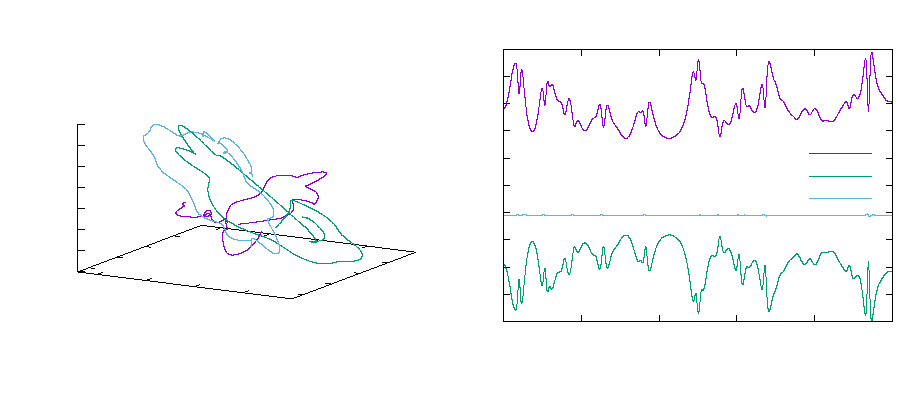
\includegraphics{MDSLP2}}%
    \gplfronttext
  \end{picture}%
\endgroup

	\caption{Trajectories (left) and plot of the kinetic, potential and total energy (right) for a system with $ N = 3 $ particles.}
	\label{fig:MDSLP2}
\end{figure}

\section{Problem 3}
The trajectories and energy plots of systems with $ N = 4 $, $ N = 5 $ and $ N = 6 $ are shown in \cref{fig:MDSLP3N4,fig:MDSLP3N5,fig:MDSLP3N6}.

\begin{figure}[h!]
	\centering
	% GNUPLOT: LaTeX picture with Postscript
\begingroup
  \makeatletter
  \providecommand\color[2][]{%
    \GenericError{(gnuplot) \space\space\space\@spaces}{%
      Package color not loaded in conjunction with
      terminal option `colourtext'%
    }{See the gnuplot documentation for explanation.%
    }{Either use 'blacktext' in gnuplot or load the package
      color.sty in LaTeX.}%
    \renewcommand\color[2][]{}%
  }%
  \providecommand\includegraphics[2][]{%
    \GenericError{(gnuplot) \space\space\space\@spaces}{%
      Package graphicx or graphics not loaded%
    }{See the gnuplot documentation for explanation.%
    }{The gnuplot epslatex terminal needs graphicx.sty or graphics.sty.}%
    \renewcommand\includegraphics[2][]{}%
  }%
  \providecommand\rotatebox[2]{#2}%
  \@ifundefined{ifGPcolor}{%
    \newif\ifGPcolor
    \GPcolorfalse
  }{}%
  \@ifundefined{ifGPblacktext}{%
    \newif\ifGPblacktext
    \GPblacktexttrue
  }{}%
  % define a \g@addto@macro without @ in the name:
  \let\gplgaddtomacro\g@addto@macro
  % define empty templates for all commands taking text:
  \gdef\gplbacktext{}%
  \gdef\gplfronttext{}%
  \makeatother
  \ifGPblacktext
    % no textcolor at all
    \def\colorrgb#1{}%
    \def\colorgray#1{}%
  \else
    % gray or color?
    \ifGPcolor
      \def\colorrgb#1{\color[rgb]{#1}}%
      \def\colorgray#1{\color[gray]{#1}}%
      \expandafter\def\csname LTw\endcsname{\color{white}}%
      \expandafter\def\csname LTb\endcsname{\color{black}}%
      \expandafter\def\csname LTa\endcsname{\color{black}}%
      \expandafter\def\csname LT0\endcsname{\color[rgb]{1,0,0}}%
      \expandafter\def\csname LT1\endcsname{\color[rgb]{0,1,0}}%
      \expandafter\def\csname LT2\endcsname{\color[rgb]{0,0,1}}%
      \expandafter\def\csname LT3\endcsname{\color[rgb]{1,0,1}}%
      \expandafter\def\csname LT4\endcsname{\color[rgb]{0,1,1}}%
      \expandafter\def\csname LT5\endcsname{\color[rgb]{1,1,0}}%
      \expandafter\def\csname LT6\endcsname{\color[rgb]{0,0,0}}%
      \expandafter\def\csname LT7\endcsname{\color[rgb]{1,0.3,0}}%
      \expandafter\def\csname LT8\endcsname{\color[rgb]{0.5,0.5,0.5}}%
    \else
      % gray
      \def\colorrgb#1{\color{black}}%
      \def\colorgray#1{\color[gray]{#1}}%
      \expandafter\def\csname LTw\endcsname{\color{white}}%
      \expandafter\def\csname LTb\endcsname{\color{black}}%
      \expandafter\def\csname LTa\endcsname{\color{black}}%
      \expandafter\def\csname LT0\endcsname{\color{black}}%
      \expandafter\def\csname LT1\endcsname{\color{black}}%
      \expandafter\def\csname LT2\endcsname{\color{black}}%
      \expandafter\def\csname LT3\endcsname{\color{black}}%
      \expandafter\def\csname LT4\endcsname{\color{black}}%
      \expandafter\def\csname LT5\endcsname{\color{black}}%
      \expandafter\def\csname LT6\endcsname{\color{black}}%
      \expandafter\def\csname LT7\endcsname{\color{black}}%
      \expandafter\def\csname LT8\endcsname{\color{black}}%
    \fi
  \fi
    \setlength{\unitlength}{0.0500bp}%
    \ifx\gptboxheight\undefined%
      \newlength{\gptboxheight}%
      \newlength{\gptboxwidth}%
      \newsavebox{\gptboxtext}%
    \fi%
    \setlength{\fboxrule}{0.5pt}%
    \setlength{\fboxsep}{1pt}%
\begin{picture}(8496.00,5040.00)%
    \gplgaddtomacro\gplbacktext{%
      \csname LTb\endcsname%
      \put(475,1695){\makebox(0,0){\strut{}$-2$}}%
      \put(770,1658){\makebox(0,0){\strut{}$-1$}}%
      \put(1064,1621){\makebox(0,0){\strut{}$0$}}%
      \put(1358,1584){\makebox(0,0){\strut{}$1$}}%
      \put(1652,1548){\makebox(0,0){\strut{}$2$}}%
      \put(1947,1511){\makebox(0,0){\strut{}$3$}}%
      \put(2240,1474){\makebox(0,0){\strut{}$4$}}%
      \put(2534,1437){\makebox(0,0){\strut{}$5$}}%
      \put(2771,1478){\makebox(0,0){\strut{}$-1$}}%
      \put(3068,1590){\makebox(0,0){\strut{}$0$}}%
      \put(3366,1702){\makebox(0,0){\strut{}$1$}}%
      \put(3663,1814){\makebox(0,0){\strut{}$2$}}%
      \put(3960,1926){\makebox(0,0){\strut{}$3$}}%
      \put(459,1983){\makebox(0,0)[r]{\strut{}$-2$}}%
      \put(459,2299){\makebox(0,0)[r]{\strut{}$-1$}}%
      \put(459,2615){\makebox(0,0)[r]{\strut{}$0$}}%
      \put(459,2930){\makebox(0,0)[r]{\strut{}$1$}}%
      \put(459,3245){\makebox(0,0)[r]{\strut{}$2$}}%
      \put(-75,2536){\makebox(0,0){\strut{}z}}%
    }%
    \gplgaddtomacro\gplfronttext{%
      \csname LTb\endcsname%
      \put(1318,1365){\makebox(0,0){\strut{}x}}%
      \put(3753,1507){\makebox(0,0){\strut{}y}}%
      \put(-75,2536){\makebox(0,0){\strut{}z}}%
    }%
    \gplgaddtomacro\gplbacktext{%
      \csname LTb\endcsname%
      \put(4540,1587){\makebox(0,0)[r]{\strut{}$-4$}}%
      \put(4540,1927){\makebox(0,0)[r]{\strut{}$-3$}}%
      \put(4540,2266){\makebox(0,0)[r]{\strut{}$-2$}}%
      \put(4540,2606){\makebox(0,0)[r]{\strut{}$-1$}}%
      \put(4540,2946){\makebox(0,0)[r]{\strut{}$0$}}%
      \put(4540,3286){\makebox(0,0)[r]{\strut{}$1$}}%
      \put(4540,3625){\makebox(0,0)[r]{\strut{}$2$}}%
      \put(4540,3965){\makebox(0,0)[r]{\strut{}$3$}}%
      \put(4672,1129){\makebox(0,0){\strut{}$0$}}%
      \put(5420,1129){\makebox(0,0){\strut{}$2$}}%
      \put(6167,1129){\makebox(0,0){\strut{}$4$}}%
      \put(6915,1129){\makebox(0,0){\strut{}$6$}}%
      \put(7662,1129){\makebox(0,0){\strut{}$8$}}%
      \put(8410,1129){\makebox(0,0){\strut{}$10$}}%
    }%
    \gplgaddtomacro\gplfronttext{%
      \csname LTb\endcsname%
      \put(4232,2657){\rotatebox{-270}{\makebox(0,0){\strut{}energy}}}%
      \put(6541,964){\makebox(0,0){\strut{}time t}}%
      \csname LTb\endcsname%
      \put(7480,3023){\makebox(0,0)[r]{\strut{}Kinetic energy}}%
      \csname LTb\endcsname%
      \put(7480,2803){\makebox(0,0)[r]{\strut{}Potential energy}}%
      \csname LTb\endcsname%
      \put(7480,2583){\makebox(0,0)[r]{\strut{}Total energy}}%
    }%
    \gplbacktext
    \put(0,0){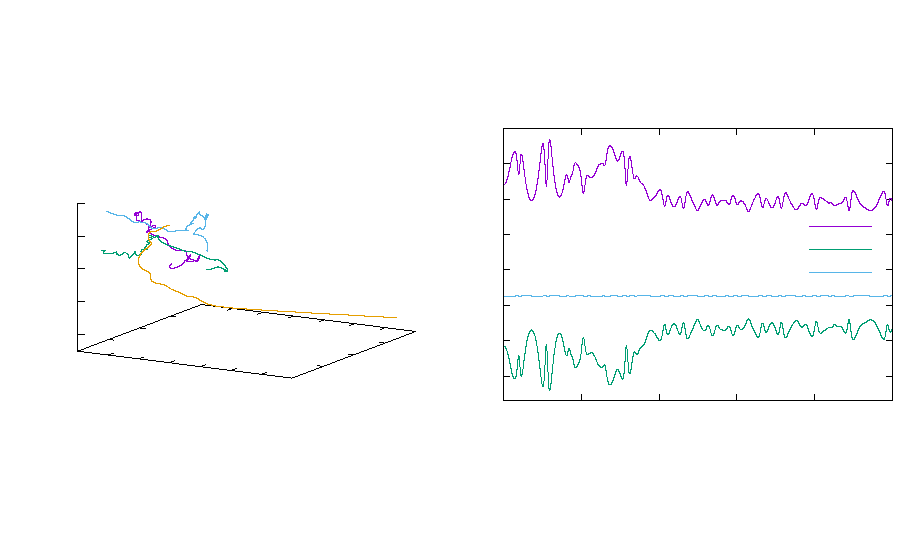
\includegraphics{MDSLP3N4}}%
    \gplfronttext
  \end{picture}%
\endgroup

	\caption{Trajectories (left) and plot of the kinetic, potential and total energy (right) for a system with $ N = 4 $ particles.}
	\label{fig:MDSLP3N4}
\end{figure}

\begin{figure}[h!]
	\centering
	% GNUPLOT: LaTeX picture with Postscript
\begingroup
  \makeatletter
  \providecommand\color[2][]{%
    \GenericError{(gnuplot) \space\space\space\@spaces}{%
      Package color not loaded in conjunction with
      terminal option `colourtext'%
    }{See the gnuplot documentation for explanation.%
    }{Either use 'blacktext' in gnuplot or load the package
      color.sty in LaTeX.}%
    \renewcommand\color[2][]{}%
  }%
  \providecommand\includegraphics[2][]{%
    \GenericError{(gnuplot) \space\space\space\@spaces}{%
      Package graphicx or graphics not loaded%
    }{See the gnuplot documentation for explanation.%
    }{The gnuplot epslatex terminal needs graphicx.sty or graphics.sty.}%
    \renewcommand\includegraphics[2][]{}%
  }%
  \providecommand\rotatebox[2]{#2}%
  \@ifundefined{ifGPcolor}{%
    \newif\ifGPcolor
    \GPcolorfalse
  }{}%
  \@ifundefined{ifGPblacktext}{%
    \newif\ifGPblacktext
    \GPblacktexttrue
  }{}%
  % define a \g@addto@macro without @ in the name:
  \let\gplgaddtomacro\g@addto@macro
  % define empty templates for all commands taking text:
  \gdef\gplbacktext{}%
  \gdef\gplfronttext{}%
  \makeatother
  \ifGPblacktext
    % no textcolor at all
    \def\colorrgb#1{}%
    \def\colorgray#1{}%
  \else
    % gray or color?
    \ifGPcolor
      \def\colorrgb#1{\color[rgb]{#1}}%
      \def\colorgray#1{\color[gray]{#1}}%
      \expandafter\def\csname LTw\endcsname{\color{white}}%
      \expandafter\def\csname LTb\endcsname{\color{black}}%
      \expandafter\def\csname LTa\endcsname{\color{black}}%
      \expandafter\def\csname LT0\endcsname{\color[rgb]{1,0,0}}%
      \expandafter\def\csname LT1\endcsname{\color[rgb]{0,1,0}}%
      \expandafter\def\csname LT2\endcsname{\color[rgb]{0,0,1}}%
      \expandafter\def\csname LT3\endcsname{\color[rgb]{1,0,1}}%
      \expandafter\def\csname LT4\endcsname{\color[rgb]{0,1,1}}%
      \expandafter\def\csname LT5\endcsname{\color[rgb]{1,1,0}}%
      \expandafter\def\csname LT6\endcsname{\color[rgb]{0,0,0}}%
      \expandafter\def\csname LT7\endcsname{\color[rgb]{1,0.3,0}}%
      \expandafter\def\csname LT8\endcsname{\color[rgb]{0.5,0.5,0.5}}%
    \else
      % gray
      \def\colorrgb#1{\color{black}}%
      \def\colorgray#1{\color[gray]{#1}}%
      \expandafter\def\csname LTw\endcsname{\color{white}}%
      \expandafter\def\csname LTb\endcsname{\color{black}}%
      \expandafter\def\csname LTa\endcsname{\color{black}}%
      \expandafter\def\csname LT0\endcsname{\color{black}}%
      \expandafter\def\csname LT1\endcsname{\color{black}}%
      \expandafter\def\csname LT2\endcsname{\color{black}}%
      \expandafter\def\csname LT3\endcsname{\color{black}}%
      \expandafter\def\csname LT4\endcsname{\color{black}}%
      \expandafter\def\csname LT5\endcsname{\color{black}}%
      \expandafter\def\csname LT6\endcsname{\color{black}}%
      \expandafter\def\csname LT7\endcsname{\color{black}}%
      \expandafter\def\csname LT8\endcsname{\color{black}}%
    \fi
  \fi
    \setlength{\unitlength}{0.0500bp}%
    \ifx\gptboxheight\undefined%
      \newlength{\gptboxheight}%
      \newlength{\gptboxwidth}%
      \newsavebox{\gptboxtext}%
    \fi%
    \setlength{\fboxrule}{0.5pt}%
    \setlength{\fboxsep}{1pt}%
\begin{picture}(8496.00,3528.00)%
    \gplgaddtomacro\gplbacktext{%
      \csname LTb\endcsname%
      \put(770,902){\makebox(0,0){\strut{}$-1$}}%
      \put(1358,828){\makebox(0,0){\strut{}$0$}}%
      \put(1947,755){\makebox(0,0){\strut{}$1$}}%
      \put(2534,681){\makebox(0,0){\strut{}$2$}}%
      \put(2771,722){\makebox(0,0){\strut{}$-1$}}%
      \put(3167,871){\makebox(0,0){\strut{}$0$}}%
      \put(3564,1021){\makebox(0,0){\strut{}$1$}}%
      \put(3960,1170){\makebox(0,0){\strut{}$2$}}%
      \put(459,1069){\makebox(0,0)[r]{\strut{}$-1$}}%
      \put(459,1475){\makebox(0,0)[r]{\strut{}$0$}}%
      \put(459,1880){\makebox(0,0)[r]{\strut{}$1$}}%
      \put(459,2286){\makebox(0,0)[r]{\strut{}$2$}}%
      \put(-75,1780){\makebox(0,0){\strut{}z}}%
    }%
    \gplgaddtomacro\gplfronttext{%
      \csname LTb\endcsname%
      \put(1318,609){\makebox(0,0){\strut{}x}}%
      \put(3753,751){\makebox(0,0){\strut{}y}}%
      \put(-75,1780){\makebox(0,0){\strut{}z}}%
    }%
    \gplgaddtomacro\gplbacktext{%
      \csname LTb\endcsname%
      \put(4540,831){\makebox(0,0)[r]{\strut{}$-6$}}%
      \put(4540,1306){\makebox(0,0)[r]{\strut{}$-4$}}%
      \put(4540,1782){\makebox(0,0)[r]{\strut{}$-2$}}%
      \put(4540,2258){\makebox(0,0)[r]{\strut{}$0$}}%
      \put(4540,2733){\makebox(0,0)[r]{\strut{}$2$}}%
      \put(4540,3209){\makebox(0,0)[r]{\strut{}$4$}}%
      \put(4672,373){\makebox(0,0){\strut{}$0$}}%
      \put(5420,373){\makebox(0,0){\strut{}$2$}}%
      \put(6167,373){\makebox(0,0){\strut{}$4$}}%
      \put(6915,373){\makebox(0,0){\strut{}$6$}}%
      \put(7662,373){\makebox(0,0){\strut{}$8$}}%
      \put(8410,373){\makebox(0,0){\strut{}$10$}}%
    }%
    \gplgaddtomacro\gplfronttext{%
      \csname LTb\endcsname%
      \put(4232,1901){\rotatebox{-270}{\makebox(0,0){\strut{}energy}}}%
      \put(6541,208){\makebox(0,0){\strut{}time t}}%
      \csname LTb\endcsname%
      \put(7480,2279){\makebox(0,0)[r]{\strut{}Kinetic energy}}%
      \csname LTb\endcsname%
      \put(7480,2059){\makebox(0,0)[r]{\strut{}Potential energy}}%
      \csname LTb\endcsname%
      \put(7480,1839){\makebox(0,0)[r]{\strut{}Total energy}}%
    }%
    \gplbacktext
    \put(0,0){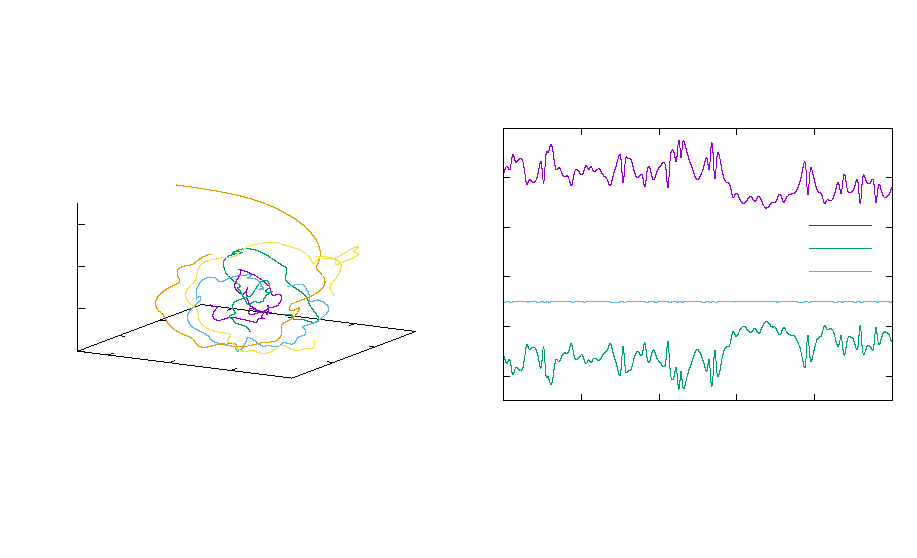
\includegraphics{MDSLP3N5}}%
    \gplfronttext
  \end{picture}%
\endgroup

	\caption{Trajectories (left) and plot of the kinetic, potential and total energy (right) for a system with $ N = 5 $ particles.}
	\label{fig:MDSLP3N5}
\end{figure}

\begin{figure}[h!]
	\centering
	%% Creator: Matplotlib, PGF backend
%%
%% To include the figure in your LaTeX document, write
%%   \input{<filename>.pgf}
%%
%% Make sure the required packages are loaded in your preamble
%%   \usepackage{pgf}
%%
%% Figures using additional raster images can only be included by \input if
%% they are in the same directory as the main LaTeX file. For loading figures
%% from other directories you can use the `import` package
%%   \usepackage{import}
%% and then include the figures with
%%   \import{<path to file>}{<filename>.pgf}
%%
%% Matplotlib used the following preamble
%%   \usepackage[utf8x]{inputenc}
%%   \usepackage[T1]{fontenc}
%%
\begingroup%
\makeatletter%
\begin{pgfpicture}%
\pgfpathrectangle{\pgfpointorigin}{\pgfqpoint{5.905512in}{2.952756in}}%
\pgfusepath{use as bounding box, clip}%
\begin{pgfscope}%
\pgfsetbuttcap%
\pgfsetmiterjoin%
\definecolor{currentfill}{rgb}{1.000000,1.000000,1.000000}%
\pgfsetfillcolor{currentfill}%
\pgfsetlinewidth{0.000000pt}%
\definecolor{currentstroke}{rgb}{1.000000,1.000000,1.000000}%
\pgfsetstrokecolor{currentstroke}%
\pgfsetdash{}{0pt}%
\pgfpathmoveto{\pgfqpoint{0.000000in}{0.000000in}}%
\pgfpathlineto{\pgfqpoint{5.905512in}{0.000000in}}%
\pgfpathlineto{\pgfqpoint{5.905512in}{2.952756in}}%
\pgfpathlineto{\pgfqpoint{0.000000in}{2.952756in}}%
\pgfpathclose%
\pgfusepath{fill}%
\end{pgfscope}%
\begin{pgfscope}%
\pgfsetbuttcap%
\pgfsetmiterjoin%
\definecolor{currentfill}{rgb}{1.000000,1.000000,1.000000}%
\pgfsetfillcolor{currentfill}%
\pgfsetlinewidth{0.000000pt}%
\definecolor{currentstroke}{rgb}{0.000000,0.000000,0.000000}%
\pgfsetstrokecolor{currentstroke}%
\pgfsetstrokeopacity{0.000000}%
\pgfsetdash{}{0pt}%
\pgfpathmoveto{\pgfqpoint{0.150000in}{0.495779in}}%
\pgfpathlineto{\pgfqpoint{2.619474in}{0.495779in}}%
\pgfpathlineto{\pgfqpoint{2.619474in}{2.753694in}}%
\pgfpathlineto{\pgfqpoint{0.150000in}{2.753694in}}%
\pgfpathclose%
\pgfusepath{fill}%
\end{pgfscope}%
\begin{pgfscope}%
\pgfsetbuttcap%
\pgfsetmiterjoin%
\definecolor{currentfill}{rgb}{0.950000,0.950000,0.950000}%
\pgfsetfillcolor{currentfill}%
\pgfsetfillopacity{0.500000}%
\pgfsetlinewidth{1.003750pt}%
\definecolor{currentstroke}{rgb}{0.950000,0.950000,0.950000}%
\pgfsetstrokecolor{currentstroke}%
\pgfsetstrokeopacity{0.500000}%
\pgfsetdash{}{0pt}%
\pgfpathmoveto{\pgfqpoint{1.183499in}{1.378348in}}%
\pgfpathlineto{\pgfqpoint{2.335057in}{1.155350in}}%
\pgfpathlineto{\pgfqpoint{2.367721in}{2.332098in}}%
\pgfpathlineto{\pgfqpoint{1.175531in}{2.507769in}}%
\pgfusepath{stroke,fill}%
\end{pgfscope}%
\begin{pgfscope}%
\pgfsetbuttcap%
\pgfsetmiterjoin%
\definecolor{currentfill}{rgb}{0.900000,0.900000,0.900000}%
\pgfsetfillcolor{currentfill}%
\pgfsetfillopacity{0.500000}%
\pgfsetlinewidth{1.003750pt}%
\definecolor{currentstroke}{rgb}{0.900000,0.900000,0.900000}%
\pgfsetstrokecolor{currentstroke}%
\pgfsetstrokeopacity{0.500000}%
\pgfsetdash{}{0pt}%
\pgfpathmoveto{\pgfqpoint{1.183499in}{1.378348in}}%
\pgfpathlineto{\pgfqpoint{0.468304in}{0.978264in}}%
\pgfpathlineto{\pgfqpoint{0.433212in}{2.192192in}}%
\pgfpathlineto{\pgfqpoint{1.175531in}{2.507769in}}%
\pgfusepath{stroke,fill}%
\end{pgfscope}%
\begin{pgfscope}%
\pgfsetbuttcap%
\pgfsetmiterjoin%
\definecolor{currentfill}{rgb}{0.925000,0.925000,0.925000}%
\pgfsetfillcolor{currentfill}%
\pgfsetfillopacity{0.500000}%
\pgfsetlinewidth{1.003750pt}%
\definecolor{currentstroke}{rgb}{0.925000,0.925000,0.925000}%
\pgfsetstrokecolor{currentstroke}%
\pgfsetstrokeopacity{0.500000}%
\pgfsetdash{}{0pt}%
\pgfpathmoveto{\pgfqpoint{1.183499in}{1.378348in}}%
\pgfpathlineto{\pgfqpoint{0.468304in}{0.978264in}}%
\pgfpathlineto{\pgfqpoint{1.685706in}{0.714796in}}%
\pgfpathlineto{\pgfqpoint{2.335057in}{1.155350in}}%
\pgfusepath{stroke,fill}%
\end{pgfscope}%
\begin{pgfscope}%
\pgfsetrectcap%
\pgfsetroundjoin%
\pgfsetlinewidth{0.752812pt}%
\definecolor{currentstroke}{rgb}{0.000000,0.000000,0.000000}%
\pgfsetstrokecolor{currentstroke}%
\pgfsetdash{}{0pt}%
\pgfpathmoveto{\pgfqpoint{2.335057in}{1.155350in}}%
\pgfpathlineto{\pgfqpoint{1.685706in}{0.714796in}}%
\pgfusepath{stroke}%
\end{pgfscope}%
\begin{pgfscope}%
\pgftext[x=2.180712in,y=0.760979in,,]{\rmfamily\fontsize{10.000000}{12.000000}\selectfont \(\displaystyle x\)}%
\end{pgfscope}%
\begin{pgfscope}%
\pgfsetbuttcap%
\pgfsetroundjoin%
\pgfsetlinewidth{1.003750pt}%
\definecolor{currentstroke}{rgb}{0.900000,0.900000,0.900000}%
\pgfsetstrokecolor{currentstroke}%
\pgfsetdash{}{0pt}%
\pgfpathmoveto{\pgfqpoint{2.226135in}{1.081452in}}%
\pgfpathlineto{\pgfqpoint{1.063132in}{1.311014in}}%
\pgfpathlineto{\pgfqpoint{1.050898in}{2.454785in}}%
\pgfusepath{stroke}%
\end{pgfscope}%
\begin{pgfscope}%
\pgfsetbuttcap%
\pgfsetroundjoin%
\pgfsetlinewidth{1.003750pt}%
\definecolor{currentstroke}{rgb}{0.900000,0.900000,0.900000}%
\pgfsetstrokecolor{currentstroke}%
\pgfsetdash{}{0pt}%
\pgfpathmoveto{\pgfqpoint{2.024235in}{0.944472in}}%
\pgfpathlineto{\pgfqpoint{0.840444in}{1.186441in}}%
\pgfpathlineto{\pgfqpoint{0.819999in}{2.356624in}}%
\pgfusepath{stroke}%
\end{pgfscope}%
\begin{pgfscope}%
\pgfsetbuttcap%
\pgfsetroundjoin%
\pgfsetlinewidth{1.003750pt}%
\definecolor{currentstroke}{rgb}{0.900000,0.900000,0.900000}%
\pgfsetstrokecolor{currentstroke}%
\pgfsetdash{}{0pt}%
\pgfpathmoveto{\pgfqpoint{1.810998in}{0.799801in}}%
\pgfpathlineto{\pgfqpoint{0.605854in}{1.055210in}}%
\pgfpathlineto{\pgfqpoint{0.576311in}{2.253027in}}%
\pgfusepath{stroke}%
\end{pgfscope}%
\begin{pgfscope}%
\pgfsetrectcap%
\pgfsetroundjoin%
\pgfsetlinewidth{1.003750pt}%
\definecolor{currentstroke}{rgb}{0.000000,0.000000,0.000000}%
\pgfsetstrokecolor{currentstroke}%
\pgfsetdash{}{0pt}%
\pgfpathmoveto{\pgfqpoint{2.216389in}{1.083376in}}%
\pgfpathlineto{\pgfqpoint{2.245651in}{1.077600in}}%
\pgfusepath{stroke}%
\end{pgfscope}%
\begin{pgfscope}%
\pgftext[x=2.292856in,y=1.003485in,,top]{\rmfamily\fontsize{8.000000}{9.600000}\selectfont \(\displaystyle 0\)}%
\end{pgfscope}%
\begin{pgfscope}%
\pgfsetrectcap%
\pgfsetroundjoin%
\pgfsetlinewidth{1.003750pt}%
\definecolor{currentstroke}{rgb}{0.000000,0.000000,0.000000}%
\pgfsetstrokecolor{currentstroke}%
\pgfsetdash{}{0pt}%
\pgfpathmoveto{\pgfqpoint{2.014302in}{0.946502in}}%
\pgfpathlineto{\pgfqpoint{2.044124in}{0.940407in}}%
\pgfusepath{stroke}%
\end{pgfscope}%
\begin{pgfscope}%
\pgftext[x=2.092627in,y=0.864271in,,top]{\rmfamily\fontsize{8.000000}{9.600000}\selectfont \(\displaystyle 1\)}%
\end{pgfscope}%
\begin{pgfscope}%
\pgfsetrectcap%
\pgfsetroundjoin%
\pgfsetlinewidth{1.003750pt}%
\definecolor{currentstroke}{rgb}{0.000000,0.000000,0.000000}%
\pgfsetstrokecolor{currentstroke}%
\pgfsetdash{}{0pt}%
\pgfpathmoveto{\pgfqpoint{1.800872in}{0.801947in}}%
\pgfpathlineto{\pgfqpoint{1.831273in}{0.795504in}}%
\pgfusepath{stroke}%
\end{pgfscope}%
\begin{pgfscope}%
\pgftext[x=1.881147in,y=0.717235in,,top]{\rmfamily\fontsize{8.000000}{9.600000}\selectfont \(\displaystyle 2\)}%
\end{pgfscope}%
\begin{pgfscope}%
\pgfsetrectcap%
\pgfsetroundjoin%
\pgfsetlinewidth{0.752812pt}%
\definecolor{currentstroke}{rgb}{0.000000,0.000000,0.000000}%
\pgfsetstrokecolor{currentstroke}%
\pgfsetdash{}{0pt}%
\pgfpathmoveto{\pgfqpoint{0.468304in}{0.978264in}}%
\pgfpathlineto{\pgfqpoint{1.685706in}{0.714796in}}%
\pgfusepath{stroke}%
\end{pgfscope}%
\begin{pgfscope}%
\pgftext[x=0.967597in,y=0.637083in,,]{\rmfamily\fontsize{10.000000}{12.000000}\selectfont \(\displaystyle y\)}%
\end{pgfscope}%
\begin{pgfscope}%
\pgfsetbuttcap%
\pgfsetroundjoin%
\pgfsetlinewidth{1.003750pt}%
\definecolor{currentstroke}{rgb}{0.900000,0.900000,0.900000}%
\pgfsetstrokecolor{currentstroke}%
\pgfsetdash{}{0pt}%
\pgfpathmoveto{\pgfqpoint{1.198284in}{2.504417in}}%
\pgfpathlineto{\pgfqpoint{1.205511in}{1.374086in}}%
\pgfpathlineto{\pgfqpoint{0.491483in}{0.973247in}}%
\pgfusepath{stroke}%
\end{pgfscope}%
\begin{pgfscope}%
\pgfsetbuttcap%
\pgfsetroundjoin%
\pgfsetlinewidth{1.003750pt}%
\definecolor{currentstroke}{rgb}{0.900000,0.900000,0.900000}%
\pgfsetstrokecolor{currentstroke}%
\pgfsetdash{}{0pt}%
\pgfpathmoveto{\pgfqpoint{1.568194in}{2.449910in}}%
\pgfpathlineto{\pgfqpoint{1.563187in}{1.304822in}}%
\pgfpathlineto{\pgfqpoint{0.868623in}{0.891628in}}%
\pgfusepath{stroke}%
\end{pgfscope}%
\begin{pgfscope}%
\pgfsetbuttcap%
\pgfsetroundjoin%
\pgfsetlinewidth{1.003750pt}%
\definecolor{currentstroke}{rgb}{0.900000,0.900000,0.900000}%
\pgfsetstrokecolor{currentstroke}%
\pgfsetdash{}{0pt}%
\pgfpathmoveto{\pgfqpoint{1.949499in}{2.393724in}}%
\pgfpathlineto{\pgfqpoint{1.931509in}{1.233496in}}%
\pgfpathlineto{\pgfqpoint{1.257971in}{0.807366in}}%
\pgfusepath{stroke}%
\end{pgfscope}%
\begin{pgfscope}%
\pgfsetbuttcap%
\pgfsetroundjoin%
\pgfsetlinewidth{1.003750pt}%
\definecolor{currentstroke}{rgb}{0.900000,0.900000,0.900000}%
\pgfsetstrokecolor{currentstroke}%
\pgfsetdash{}{0pt}%
\pgfpathmoveto{\pgfqpoint{2.342735in}{2.335780in}}%
\pgfpathlineto{\pgfqpoint{2.310960in}{1.160016in}}%
\pgfpathlineto{\pgfqpoint{1.660131in}{0.720331in}}%
\pgfusepath{stroke}%
\end{pgfscope}%
\begin{pgfscope}%
\pgfsetrectcap%
\pgfsetroundjoin%
\pgfsetlinewidth{1.003750pt}%
\definecolor{currentstroke}{rgb}{0.000000,0.000000,0.000000}%
\pgfsetstrokecolor{currentstroke}%
\pgfsetdash{}{0pt}%
\pgfpathmoveto{\pgfqpoint{0.497676in}{0.976724in}}%
\pgfpathlineto{\pgfqpoint{0.479073in}{0.966280in}}%
\pgfusepath{stroke}%
\end{pgfscope}%
\begin{pgfscope}%
\pgftext[x=0.449841in,y=0.883035in,,top]{\rmfamily\fontsize{8.000000}{9.600000}\selectfont \(\displaystyle -1\)}%
\end{pgfscope}%
\begin{pgfscope}%
\pgfsetrectcap%
\pgfsetroundjoin%
\pgfsetlinewidth{1.003750pt}%
\definecolor{currentstroke}{rgb}{0.000000,0.000000,0.000000}%
\pgfsetstrokecolor{currentstroke}%
\pgfsetdash{}{0pt}%
\pgfpathmoveto{\pgfqpoint{0.874654in}{0.895216in}}%
\pgfpathlineto{\pgfqpoint{0.856535in}{0.884437in}}%
\pgfusepath{stroke}%
\end{pgfscope}%
\begin{pgfscope}%
\pgftext[x=0.827373in,y=0.799745in,,top]{\rmfamily\fontsize{8.000000}{9.600000}\selectfont \(\displaystyle 0\)}%
\end{pgfscope}%
\begin{pgfscope}%
\pgfsetrectcap%
\pgfsetroundjoin%
\pgfsetlinewidth{1.003750pt}%
\definecolor{currentstroke}{rgb}{0.000000,0.000000,0.000000}%
\pgfsetstrokecolor{currentstroke}%
\pgfsetdash{}{0pt}%
\pgfpathmoveto{\pgfqpoint{1.263828in}{0.811071in}}%
\pgfpathlineto{\pgfqpoint{1.246234in}{0.799940in}}%
\pgfusepath{stroke}%
\end{pgfscope}%
\begin{pgfscope}%
\pgftext[x=1.217163in,y=0.713751in,,top]{\rmfamily\fontsize{8.000000}{9.600000}\selectfont \(\displaystyle 1\)}%
\end{pgfscope}%
\begin{pgfscope}%
\pgfsetrectcap%
\pgfsetroundjoin%
\pgfsetlinewidth{1.003750pt}%
\definecolor{currentstroke}{rgb}{0.000000,0.000000,0.000000}%
\pgfsetstrokecolor{currentstroke}%
\pgfsetdash{}{0pt}%
\pgfpathmoveto{\pgfqpoint{1.665797in}{0.724159in}}%
\pgfpathlineto{\pgfqpoint{1.648774in}{0.712659in}}%
\pgfusepath{stroke}%
\end{pgfscope}%
\begin{pgfscope}%
\pgftext[x=1.619815in,y=0.624920in,,top]{\rmfamily\fontsize{8.000000}{9.600000}\selectfont \(\displaystyle 2\)}%
\end{pgfscope}%
\begin{pgfscope}%
\pgfsetrectcap%
\pgfsetroundjoin%
\pgfsetlinewidth{0.752812pt}%
\definecolor{currentstroke}{rgb}{0.000000,0.000000,0.000000}%
\pgfsetstrokecolor{currentstroke}%
\pgfsetdash{}{0pt}%
\pgfpathmoveto{\pgfqpoint{0.468304in}{0.978264in}}%
\pgfpathlineto{\pgfqpoint{0.433212in}{2.192192in}}%
\pgfusepath{stroke}%
\end{pgfscope}%
\begin{pgfscope}%
\pgftext[x=0.197818in,y=1.552997in,,]{\rmfamily\fontsize{10.000000}{12.000000}\selectfont \(\displaystyle z\)}%
\end{pgfscope}%
\begin{pgfscope}%
\pgfsetbuttcap%
\pgfsetroundjoin%
\pgfsetlinewidth{1.003750pt}%
\definecolor{currentstroke}{rgb}{0.900000,0.900000,0.900000}%
\pgfsetstrokecolor{currentstroke}%
\pgfsetdash{}{0pt}%
\pgfpathmoveto{\pgfqpoint{0.462173in}{1.190346in}}%
\pgfpathlineto{\pgfqpoint{1.182104in}{1.576136in}}%
\pgfpathlineto{\pgfqpoint{2.340769in}{1.361153in}}%
\pgfusepath{stroke}%
\end{pgfscope}%
\begin{pgfscope}%
\pgfsetbuttcap%
\pgfsetroundjoin%
\pgfsetlinewidth{1.003750pt}%
\definecolor{currentstroke}{rgb}{0.900000,0.900000,0.900000}%
\pgfsetstrokecolor{currentstroke}%
\pgfsetdash{}{0pt}%
\pgfpathmoveto{\pgfqpoint{0.451076in}{1.574219in}}%
\pgfpathlineto{\pgfqpoint{1.179582in}{1.933630in}}%
\pgfpathlineto{\pgfqpoint{2.351103in}{1.733427in}}%
\pgfusepath{stroke}%
\end{pgfscope}%
\begin{pgfscope}%
\pgfsetbuttcap%
\pgfsetroundjoin%
\pgfsetlinewidth{1.003750pt}%
\definecolor{currentstroke}{rgb}{0.900000,0.900000,0.900000}%
\pgfsetstrokecolor{currentstroke}%
\pgfsetdash{}{0pt}%
\pgfpathmoveto{\pgfqpoint{0.439719in}{1.967109in}}%
\pgfpathlineto{\pgfqpoint{1.177005in}{2.298846in}}%
\pgfpathlineto{\pgfqpoint{2.361671in}{2.114135in}}%
\pgfusepath{stroke}%
\end{pgfscope}%
\begin{pgfscope}%
\pgfsetrectcap%
\pgfsetroundjoin%
\pgfsetlinewidth{1.003750pt}%
\definecolor{currentstroke}{rgb}{0.000000,0.000000,0.000000}%
\pgfsetstrokecolor{currentstroke}%
\pgfsetdash{}{0pt}%
\pgfpathmoveto{\pgfqpoint{0.468420in}{1.193693in}}%
\pgfpathlineto{\pgfqpoint{0.449655in}{1.183637in}}%
\pgfusepath{stroke}%
\end{pgfscope}%
\begin{pgfscope}%
\pgftext[x=0.352958in,y=1.180415in,right,top]{\rmfamily\fontsize{8.000000}{9.600000}\selectfont \(\displaystyle 0\)}%
\end{pgfscope}%
\begin{pgfscope}%
\pgfsetrectcap%
\pgfsetroundjoin%
\pgfsetlinewidth{1.003750pt}%
\definecolor{currentstroke}{rgb}{0.000000,0.000000,0.000000}%
\pgfsetstrokecolor{currentstroke}%
\pgfsetdash{}{0pt}%
\pgfpathmoveto{\pgfqpoint{0.457403in}{1.577340in}}%
\pgfpathlineto{\pgfqpoint{0.438397in}{1.567963in}}%
\pgfusepath{stroke}%
\end{pgfscope}%
\begin{pgfscope}%
\pgftext[x=0.340567in,y=1.564959in,right,top]{\rmfamily\fontsize{8.000000}{9.600000}\selectfont \(\displaystyle 1\)}%
\end{pgfscope}%
\begin{pgfscope}%
\pgfsetrectcap%
\pgfsetroundjoin%
\pgfsetlinewidth{1.003750pt}%
\definecolor{currentstroke}{rgb}{0.000000,0.000000,0.000000}%
\pgfsetstrokecolor{currentstroke}%
\pgfsetdash{}{0pt}%
\pgfpathmoveto{\pgfqpoint{0.446128in}{1.969992in}}%
\pgfpathlineto{\pgfqpoint{0.426874in}{1.961329in}}%
\pgfusepath{stroke}%
\end{pgfscope}%
\begin{pgfscope}%
\pgftext[x=0.327885in,y=1.958554in,right,top]{\rmfamily\fontsize{8.000000}{9.600000}\selectfont \(\displaystyle 2\)}%
\end{pgfscope}%
\begin{pgfscope}%
\pgfpathrectangle{\pgfqpoint{0.150000in}{0.495779in}}{\pgfqpoint{2.469474in}{2.257914in}} %
\pgfusepath{clip}%
\pgfsetrectcap%
\pgfsetroundjoin%
\pgfsetlinewidth{1.003750pt}%
\definecolor{currentstroke}{rgb}{0.000000,0.000000,1.000000}%
\pgfsetstrokecolor{currentstroke}%
\pgfsetdash{}{0pt}%
\pgfpathmoveto{\pgfqpoint{1.446594in}{1.438299in}}%
\pgfpathlineto{\pgfqpoint{1.436346in}{1.432866in}}%
\pgfpathlineto{\pgfqpoint{1.426903in}{1.428377in}}%
\pgfpathlineto{\pgfqpoint{1.419273in}{1.425227in}}%
\pgfpathlineto{\pgfqpoint{1.413250in}{1.423207in}}%
\pgfpathlineto{\pgfqpoint{1.408360in}{1.422039in}}%
\pgfpathlineto{\pgfqpoint{1.403703in}{1.421389in}}%
\pgfpathlineto{\pgfqpoint{1.397946in}{1.421074in}}%
\pgfpathlineto{\pgfqpoint{1.387123in}{1.421056in}}%
\pgfpathlineto{\pgfqpoint{1.376589in}{1.420857in}}%
\pgfpathlineto{\pgfqpoint{1.368617in}{1.420248in}}%
\pgfpathlineto{\pgfqpoint{1.361076in}{1.419196in}}%
\pgfpathlineto{\pgfqpoint{1.353747in}{1.417703in}}%
\pgfpathlineto{\pgfqpoint{1.346269in}{1.415720in}}%
\pgfpathlineto{\pgfqpoint{1.338227in}{1.413128in}}%
\pgfpathlineto{\pgfqpoint{1.329205in}{1.409753in}}%
\pgfpathlineto{\pgfqpoint{1.318354in}{1.405204in}}%
\pgfpathlineto{\pgfqpoint{1.304563in}{1.398926in}}%
\pgfpathlineto{\pgfqpoint{1.278688in}{1.386549in}}%
\pgfpathlineto{\pgfqpoint{1.257833in}{1.376774in}}%
\pgfpathlineto{\pgfqpoint{1.245517in}{1.371453in}}%
\pgfpathlineto{\pgfqpoint{1.236852in}{1.368153in}}%
\pgfpathlineto{\pgfqpoint{1.230608in}{1.366206in}}%
\pgfpathlineto{\pgfqpoint{1.226127in}{1.365242in}}%
\pgfpathlineto{\pgfqpoint{1.223165in}{1.365019in}}%
\pgfpathlineto{\pgfqpoint{1.221255in}{1.365289in}}%
\pgfpathlineto{\pgfqpoint{1.220136in}{1.365873in}}%
\pgfpathlineto{\pgfqpoint{1.219558in}{1.366671in}}%
\pgfpathlineto{\pgfqpoint{1.219387in}{1.367728in}}%
\pgfpathlineto{\pgfqpoint{1.219654in}{1.369129in}}%
\pgfpathlineto{\pgfqpoint{1.220499in}{1.371024in}}%
\pgfpathlineto{\pgfqpoint{1.222186in}{1.373637in}}%
\pgfpathlineto{\pgfqpoint{1.225116in}{1.377283in}}%
\pgfpathlineto{\pgfqpoint{1.231035in}{1.383774in}}%
\pgfpathlineto{\pgfqpoint{1.235959in}{1.389424in}}%
\pgfpathlineto{\pgfqpoint{1.238246in}{1.392684in}}%
\pgfpathlineto{\pgfqpoint{1.239546in}{1.395234in}}%
\pgfpathlineto{\pgfqpoint{1.240219in}{1.397426in}}%
\pgfpathlineto{\pgfqpoint{1.240417in}{1.399450in}}%
\pgfpathlineto{\pgfqpoint{1.240164in}{1.401523in}}%
\pgfpathlineto{\pgfqpoint{1.239412in}{1.403644in}}%
\pgfpathlineto{\pgfqpoint{1.238144in}{1.405815in}}%
\pgfpathlineto{\pgfqpoint{1.236137in}{1.408283in}}%
\pgfpathlineto{\pgfqpoint{1.233263in}{1.411063in}}%
\pgfpathlineto{\pgfqpoint{1.229110in}{1.414423in}}%
\pgfpathlineto{\pgfqpoint{1.223163in}{1.418626in}}%
\pgfpathlineto{\pgfqpoint{1.215754in}{1.423321in}}%
\pgfpathlineto{\pgfqpoint{1.208731in}{1.427275in}}%
\pgfpathlineto{\pgfqpoint{1.202723in}{1.430158in}}%
\pgfpathlineto{\pgfqpoint{1.197369in}{1.432246in}}%
\pgfpathlineto{\pgfqpoint{1.192240in}{1.433793in}}%
\pgfpathlineto{\pgfqpoint{1.186835in}{1.434969in}}%
\pgfpathlineto{\pgfqpoint{1.180584in}{1.435836in}}%
\pgfpathlineto{\pgfqpoint{1.173467in}{1.436325in}}%
\pgfpathlineto{\pgfqpoint{1.164927in}{1.436420in}}%
\pgfpathlineto{\pgfqpoint{1.153886in}{1.436055in}}%
\pgfpathlineto{\pgfqpoint{1.137267in}{1.435005in}}%
\pgfpathlineto{\pgfqpoint{1.091172in}{1.431918in}}%
\pgfpathlineto{\pgfqpoint{1.067839in}{1.430926in}}%
\pgfpathlineto{\pgfqpoint{1.046968in}{1.430445in}}%
\pgfpathlineto{\pgfqpoint{1.032759in}{1.430498in}}%
\pgfpathlineto{\pgfqpoint{1.024960in}{1.430928in}}%
\pgfpathlineto{\pgfqpoint{1.022071in}{1.431447in}}%
\pgfpathlineto{\pgfqpoint{1.021709in}{1.431811in}}%
\pgfpathlineto{\pgfqpoint{1.021717in}{1.431826in}}%
\pgfpathlineto{\pgfqpoint{1.022125in}{1.432089in}}%
\pgfpathlineto{\pgfqpoint{1.023774in}{1.432510in}}%
\pgfpathlineto{\pgfqpoint{1.028913in}{1.433238in}}%
\pgfpathlineto{\pgfqpoint{1.039447in}{1.434747in}}%
\pgfpathlineto{\pgfqpoint{1.043577in}{1.435800in}}%
\pgfpathlineto{\pgfqpoint{1.046307in}{1.436939in}}%
\pgfpathlineto{\pgfqpoint{1.048086in}{1.438138in}}%
\pgfpathlineto{\pgfqpoint{1.049306in}{1.439502in}}%
\pgfpathlineto{\pgfqpoint{1.050028in}{1.440982in}}%
\pgfpathlineto{\pgfqpoint{1.050374in}{1.442699in}}%
\pgfpathlineto{\pgfqpoint{1.050339in}{1.444858in}}%
\pgfpathlineto{\pgfqpoint{1.049820in}{1.447749in}}%
\pgfpathlineto{\pgfqpoint{1.048496in}{1.452275in}}%
\pgfpathlineto{\pgfqpoint{1.044568in}{1.465014in}}%
\pgfpathlineto{\pgfqpoint{1.043483in}{1.470270in}}%
\pgfpathlineto{\pgfqpoint{1.042897in}{1.475284in}}%
\pgfpathlineto{\pgfqpoint{1.042792in}{1.480006in}}%
\pgfpathlineto{\pgfqpoint{1.043118in}{1.484411in}}%
\pgfpathlineto{\pgfqpoint{1.043874in}{1.488800in}}%
\pgfpathlineto{\pgfqpoint{1.045075in}{1.493161in}}%
\pgfpathlineto{\pgfqpoint{1.046733in}{1.497488in}}%
\pgfpathlineto{\pgfqpoint{1.048860in}{1.501774in}}%
\pgfpathlineto{\pgfqpoint{1.051465in}{1.506012in}}%
\pgfpathlineto{\pgfqpoint{1.054556in}{1.510199in}}%
\pgfpathlineto{\pgfqpoint{1.058142in}{1.514333in}}%
\pgfpathlineto{\pgfqpoint{1.062542in}{1.518702in}}%
\pgfpathlineto{\pgfqpoint{1.067527in}{1.523006in}}%
\pgfpathlineto{\pgfqpoint{1.073102in}{1.527248in}}%
\pgfpathlineto{\pgfqpoint{1.079708in}{1.531701in}}%
\pgfpathlineto{\pgfqpoint{1.086992in}{1.536074in}}%
\pgfpathlineto{\pgfqpoint{1.094946in}{1.540354in}}%
\pgfpathlineto{\pgfqpoint{1.104093in}{1.544764in}}%
\pgfpathlineto{\pgfqpoint{1.113867in}{1.548962in}}%
\pgfpathlineto{\pgfqpoint{1.123471in}{1.552603in}}%
\pgfpathlineto{\pgfqpoint{1.132579in}{1.555582in}}%
\pgfpathlineto{\pgfqpoint{1.140260in}{1.557652in}}%
\pgfpathlineto{\pgfqpoint{1.146865in}{1.558975in}}%
\pgfpathlineto{\pgfqpoint{1.151766in}{1.559534in}}%
\pgfpathlineto{\pgfqpoint{1.155516in}{1.559541in}}%
\pgfpathlineto{\pgfqpoint{1.158192in}{1.559116in}}%
\pgfpathlineto{\pgfqpoint{1.159942in}{1.558399in}}%
\pgfpathlineto{\pgfqpoint{1.160958in}{1.557527in}}%
\pgfpathlineto{\pgfqpoint{1.161504in}{1.556425in}}%
\pgfpathlineto{\pgfqpoint{1.161569in}{1.555102in}}%
\pgfpathlineto{\pgfqpoint{1.161159in}{1.553575in}}%
\pgfpathlineto{\pgfqpoint{1.160106in}{1.551564in}}%
\pgfpathlineto{\pgfqpoint{1.158215in}{1.549008in}}%
\pgfpathlineto{\pgfqpoint{1.154985in}{1.545520in}}%
\pgfpathlineto{\pgfqpoint{1.150161in}{1.541067in}}%
\pgfpathlineto{\pgfqpoint{1.143712in}{1.535753in}}%
\pgfpathlineto{\pgfqpoint{1.135814in}{1.529830in}}%
\pgfpathlineto{\pgfqpoint{1.127749in}{1.524318in}}%
\pgfpathlineto{\pgfqpoint{1.119728in}{1.519363in}}%
\pgfpathlineto{\pgfqpoint{1.111852in}{1.515018in}}%
\pgfpathlineto{\pgfqpoint{1.103701in}{1.511039in}}%
\pgfpathlineto{\pgfqpoint{1.094918in}{1.507263in}}%
\pgfpathlineto{\pgfqpoint{1.084422in}{1.503257in}}%
\pgfpathlineto{\pgfqpoint{1.054808in}{1.492272in}}%
\pgfpathlineto{\pgfqpoint{1.048439in}{1.489249in}}%
\pgfpathlineto{\pgfqpoint{1.043500in}{1.486415in}}%
\pgfpathlineto{\pgfqpoint{1.039753in}{1.483766in}}%
\pgfpathlineto{\pgfqpoint{1.036845in}{1.481178in}}%
\pgfpathlineto{\pgfqpoint{1.034668in}{1.478660in}}%
\pgfpathlineto{\pgfqpoint{1.033127in}{1.476222in}}%
\pgfpathlineto{\pgfqpoint{1.032082in}{1.473727in}}%
\pgfpathlineto{\pgfqpoint{1.031548in}{1.471331in}}%
\pgfpathlineto{\pgfqpoint{1.031450in}{1.468890in}}%
\pgfpathlineto{\pgfqpoint{1.031785in}{1.466408in}}%
\pgfpathlineto{\pgfqpoint{1.032615in}{1.463730in}}%
\pgfpathlineto{\pgfqpoint{1.033933in}{1.461016in}}%
\pgfpathlineto{\pgfqpoint{1.035857in}{1.458111in}}%
\pgfpathlineto{\pgfqpoint{1.038474in}{1.455021in}}%
\pgfpathlineto{\pgfqpoint{1.041867in}{1.451760in}}%
\pgfpathlineto{\pgfqpoint{1.045892in}{1.448516in}}%
\pgfpathlineto{\pgfqpoint{1.050752in}{1.445174in}}%
\pgfpathlineto{\pgfqpoint{1.056446in}{1.441817in}}%
\pgfpathlineto{\pgfqpoint{1.062596in}{1.438730in}}%
\pgfpathlineto{\pgfqpoint{1.068669in}{1.436191in}}%
\pgfpathlineto{\pgfqpoint{1.074101in}{1.434399in}}%
\pgfpathlineto{\pgfqpoint{1.078730in}{1.433324in}}%
\pgfpathlineto{\pgfqpoint{1.082531in}{1.432860in}}%
\pgfpathlineto{\pgfqpoint{1.086029in}{1.432880in}}%
\pgfpathlineto{\pgfqpoint{1.089040in}{1.433331in}}%
\pgfpathlineto{\pgfqpoint{1.092065in}{1.434240in}}%
\pgfpathlineto{\pgfqpoint{1.095384in}{1.435732in}}%
\pgfpathlineto{\pgfqpoint{1.100008in}{1.438356in}}%
\pgfpathlineto{\pgfqpoint{1.111664in}{1.445132in}}%
\pgfpathlineto{\pgfqpoint{1.118253in}{1.448367in}}%
\pgfpathlineto{\pgfqpoint{1.124145in}{1.450780in}}%
\pgfpathlineto{\pgfqpoint{1.129242in}{1.452408in}}%
\pgfpathlineto{\pgfqpoint{1.133639in}{1.453342in}}%
\pgfpathlineto{\pgfqpoint{1.137219in}{1.453639in}}%
\pgfpathlineto{\pgfqpoint{1.139976in}{1.453453in}}%
\pgfpathlineto{\pgfqpoint{1.142252in}{1.452911in}}%
\pgfpathlineto{\pgfqpoint{1.144335in}{1.451981in}}%
\pgfpathlineto{\pgfqpoint{1.146211in}{1.450645in}}%
\pgfpathlineto{\pgfqpoint{1.147880in}{1.448902in}}%
\pgfpathlineto{\pgfqpoint{1.149530in}{1.446476in}}%
\pgfpathlineto{\pgfqpoint{1.151126in}{1.443257in}}%
\pgfpathlineto{\pgfqpoint{1.152805in}{1.438783in}}%
\pgfpathlineto{\pgfqpoint{1.155106in}{1.431152in}}%
\pgfpathlineto{\pgfqpoint{1.160537in}{1.412770in}}%
\pgfpathlineto{\pgfqpoint{1.164081in}{1.402603in}}%
\pgfpathlineto{\pgfqpoint{1.168400in}{1.391575in}}%
\pgfpathlineto{\pgfqpoint{1.177242in}{1.370558in}}%
\pgfpathlineto{\pgfqpoint{1.183841in}{1.354178in}}%
\pgfpathlineto{\pgfqpoint{1.196605in}{1.321859in}}%
\pgfpathlineto{\pgfqpoint{1.201121in}{1.312044in}}%
\pgfpathlineto{\pgfqpoint{1.205644in}{1.303306in}}%
\pgfpathlineto{\pgfqpoint{1.210343in}{1.295217in}}%
\pgfpathlineto{\pgfqpoint{1.215414in}{1.287378in}}%
\pgfpathlineto{\pgfqpoint{1.221351in}{1.279052in}}%
\pgfpathlineto{\pgfqpoint{1.229766in}{1.268118in}}%
\pgfpathlineto{\pgfqpoint{1.241573in}{1.252684in}}%
\pgfpathlineto{\pgfqpoint{1.259705in}{1.228337in}}%
\pgfpathlineto{\pgfqpoint{1.265620in}{1.221408in}}%
\pgfpathlineto{\pgfqpoint{1.271563in}{1.215125in}}%
\pgfpathlineto{\pgfqpoint{1.277830in}{1.209171in}}%
\pgfpathlineto{\pgfqpoint{1.284057in}{1.203853in}}%
\pgfpathlineto{\pgfqpoint{1.290922in}{1.198585in}}%
\pgfpathlineto{\pgfqpoint{1.298060in}{1.193670in}}%
\pgfpathlineto{\pgfqpoint{1.305842in}{1.188871in}}%
\pgfpathlineto{\pgfqpoint{1.313862in}{1.184444in}}%
\pgfpathlineto{\pgfqpoint{1.322501in}{1.180180in}}%
\pgfpathlineto{\pgfqpoint{1.331747in}{1.176118in}}%
\pgfpathlineto{\pgfqpoint{1.341582in}{1.172294in}}%
\pgfpathlineto{\pgfqpoint{1.351979in}{1.168742in}}%
\pgfpathlineto{\pgfqpoint{1.362911in}{1.165495in}}%
\pgfpathlineto{\pgfqpoint{1.373906in}{1.162691in}}%
\pgfpathlineto{\pgfqpoint{1.385373in}{1.160226in}}%
\pgfpathlineto{\pgfqpoint{1.397283in}{1.158138in}}%
\pgfpathlineto{\pgfqpoint{1.409169in}{1.156516in}}%
\pgfpathlineto{\pgfqpoint{1.421008in}{1.155349in}}%
\pgfpathlineto{\pgfqpoint{1.432783in}{1.154630in}}%
\pgfpathlineto{\pgfqpoint{1.444479in}{1.154353in}}%
\pgfpathlineto{\pgfqpoint{1.456082in}{1.154513in}}%
\pgfpathlineto{\pgfqpoint{1.467580in}{1.155109in}}%
\pgfpathlineto{\pgfqpoint{1.478962in}{1.156143in}}%
\pgfpathlineto{\pgfqpoint{1.490215in}{1.157619in}}%
\pgfpathlineto{\pgfqpoint{1.500919in}{1.159466in}}%
\pgfpathlineto{\pgfqpoint{1.511481in}{1.161741in}}%
\pgfpathlineto{\pgfqpoint{1.521490in}{1.164344in}}%
\pgfpathlineto{\pgfqpoint{1.531342in}{1.167372in}}%
\pgfpathlineto{\pgfqpoint{1.540640in}{1.170688in}}%
\pgfpathlineto{\pgfqpoint{1.549766in}{1.174419in}}%
\pgfpathlineto{\pgfqpoint{1.558710in}{1.178570in}}%
\pgfpathlineto{\pgfqpoint{1.567103in}{1.182946in}}%
\pgfpathlineto{\pgfqpoint{1.575315in}{1.187712in}}%
\pgfpathlineto{\pgfqpoint{1.583343in}{1.192865in}}%
\pgfpathlineto{\pgfqpoint{1.591521in}{1.198657in}}%
\pgfpathlineto{\pgfqpoint{1.599496in}{1.204871in}}%
\pgfpathlineto{\pgfqpoint{1.607262in}{1.211509in}}%
\pgfpathlineto{\pgfqpoint{1.614818in}{1.218576in}}%
\pgfpathlineto{\pgfqpoint{1.622160in}{1.226076in}}%
\pgfpathlineto{\pgfqpoint{1.629281in}{1.234020in}}%
\pgfpathlineto{\pgfqpoint{1.635892in}{1.242059in}}%
\pgfpathlineto{\pgfqpoint{1.642286in}{1.250529in}}%
\pgfpathlineto{\pgfqpoint{1.648452in}{1.259445in}}%
\pgfpathlineto{\pgfqpoint{1.654379in}{1.268822in}}%
\pgfpathlineto{\pgfqpoint{1.660054in}{1.278669in}}%
\pgfpathlineto{\pgfqpoint{1.665467in}{1.288971in}}%
\pgfpathlineto{\pgfqpoint{1.671274in}{1.301049in}}%
\pgfpathlineto{\pgfqpoint{1.682301in}{1.324423in}}%
\pgfpathlineto{\pgfqpoint{1.684951in}{1.328801in}}%
\pgfpathlineto{\pgfqpoint{1.687284in}{1.331840in}}%
\pgfpathlineto{\pgfqpoint{1.689515in}{1.334005in}}%
\pgfpathlineto{\pgfqpoint{1.691620in}{1.335433in}}%
\pgfpathlineto{\pgfqpoint{1.693848in}{1.336389in}}%
\pgfpathlineto{\pgfqpoint{1.696197in}{1.336894in}}%
\pgfpathlineto{\pgfqpoint{1.698969in}{1.336980in}}%
\pgfpathlineto{\pgfqpoint{1.702183in}{1.336578in}}%
\pgfpathlineto{\pgfqpoint{1.706167in}{1.335585in}}%
\pgfpathlineto{\pgfqpoint{1.711577in}{1.333730in}}%
\pgfpathlineto{\pgfqpoint{1.721906in}{1.329597in}}%
\pgfpathlineto{\pgfqpoint{1.734179in}{1.324861in}}%
\pgfpathlineto{\pgfqpoint{1.742572in}{1.322120in}}%
\pgfpathlineto{\pgfqpoint{1.749881in}{1.320216in}}%
\pgfpathlineto{\pgfqpoint{1.755865in}{1.319109in}}%
\pgfpathlineto{\pgfqpoint{1.760573in}{1.318667in}}%
\pgfpathlineto{\pgfqpoint{1.763943in}{1.318775in}}%
\pgfpathlineto{\pgfqpoint{1.766062in}{1.319272in}}%
\pgfpathlineto{\pgfqpoint{1.767120in}{1.319928in}}%
\pgfpathlineto{\pgfqpoint{1.767579in}{1.320710in}}%
\pgfpathlineto{\pgfqpoint{1.767576in}{1.321614in}}%
\pgfpathlineto{\pgfqpoint{1.767098in}{1.322754in}}%
\pgfpathlineto{\pgfqpoint{1.765907in}{1.324333in}}%
\pgfpathlineto{\pgfqpoint{1.763616in}{1.326566in}}%
\pgfpathlineto{\pgfqpoint{1.758314in}{1.330964in}}%
\pgfpathlineto{\pgfqpoint{1.753998in}{1.334797in}}%
\pgfpathlineto{\pgfqpoint{1.751753in}{1.337378in}}%
\pgfpathlineto{\pgfqpoint{1.750491in}{1.339476in}}%
\pgfpathlineto{\pgfqpoint{1.749803in}{1.341487in}}%
\pgfpathlineto{\pgfqpoint{1.749604in}{1.343397in}}%
\pgfpathlineto{\pgfqpoint{1.749826in}{1.345528in}}%
\pgfpathlineto{\pgfqpoint{1.750579in}{1.348242in}}%
\pgfpathlineto{\pgfqpoint{1.753087in}{1.354863in}}%
\pgfpathlineto{\pgfqpoint{1.756157in}{1.362807in}}%
\pgfpathlineto{\pgfqpoint{1.756862in}{1.363196in}}%
\pgfpathlineto{\pgfqpoint{1.757644in}{1.363122in}}%
\pgfpathlineto{\pgfqpoint{1.758829in}{1.362515in}}%
\pgfpathlineto{\pgfqpoint{1.761512in}{1.360465in}}%
\pgfpathlineto{\pgfqpoint{1.766739in}{1.356539in}}%
\pgfpathlineto{\pgfqpoint{1.771031in}{1.353908in}}%
\pgfpathlineto{\pgfqpoint{1.775603in}{1.351620in}}%
\pgfpathlineto{\pgfqpoint{1.780801in}{1.349529in}}%
\pgfpathlineto{\pgfqpoint{1.785895in}{1.347950in}}%
\pgfpathlineto{\pgfqpoint{1.788984in}{1.347380in}}%
\pgfpathlineto{\pgfqpoint{1.789309in}{1.347497in}}%
\pgfpathlineto{\pgfqpoint{1.789250in}{1.347606in}}%
\pgfpathlineto{\pgfqpoint{1.788459in}{1.348106in}}%
\pgfpathlineto{\pgfqpoint{1.785454in}{1.349395in}}%
\pgfpathlineto{\pgfqpoint{1.777515in}{1.352257in}}%
\pgfpathlineto{\pgfqpoint{1.762370in}{1.357217in}}%
\pgfpathlineto{\pgfqpoint{1.750174in}{1.360804in}}%
\pgfpathlineto{\pgfqpoint{1.742983in}{1.362487in}}%
\pgfpathlineto{\pgfqpoint{1.736933in}{1.363446in}}%
\pgfpathlineto{\pgfqpoint{1.726349in}{1.364536in}}%
\pgfpathlineto{\pgfqpoint{1.719624in}{1.364956in}}%
\pgfpathlineto{\pgfqpoint{1.717336in}{1.364712in}}%
\pgfpathlineto{\pgfqpoint{1.716386in}{1.364248in}}%
\pgfpathlineto{\pgfqpoint{1.716046in}{1.363656in}}%
\pgfpathlineto{\pgfqpoint{1.716128in}{1.362820in}}%
\pgfpathlineto{\pgfqpoint{1.716806in}{1.361532in}}%
\pgfpathlineto{\pgfqpoint{1.718353in}{1.359631in}}%
\pgfpathlineto{\pgfqpoint{1.721659in}{1.356386in}}%
\pgfpathlineto{\pgfqpoint{1.727846in}{1.351041in}}%
\pgfpathlineto{\pgfqpoint{1.740699in}{1.340660in}}%
\pgfpathlineto{\pgfqpoint{1.768934in}{1.317917in}}%
\pgfpathlineto{\pgfqpoint{1.782385in}{1.306503in}}%
\pgfpathlineto{\pgfqpoint{1.792538in}{1.297331in}}%
\pgfpathlineto{\pgfqpoint{1.799626in}{1.290359in}}%
\pgfpathlineto{\pgfqpoint{1.803990in}{1.285511in}}%
\pgfpathlineto{\pgfqpoint{1.806485in}{1.282154in}}%
\pgfpathlineto{\pgfqpoint{1.807579in}{1.280024in}}%
\pgfpathlineto{\pgfqpoint{1.807785in}{1.278760in}}%
\pgfpathlineto{\pgfqpoint{1.807475in}{1.278037in}}%
\pgfpathlineto{\pgfqpoint{1.806788in}{1.277638in}}%
\pgfpathlineto{\pgfqpoint{1.805549in}{1.277502in}}%
\pgfpathlineto{\pgfqpoint{1.803346in}{1.277781in}}%
\pgfpathlineto{\pgfqpoint{1.799446in}{1.278798in}}%
\pgfpathlineto{\pgfqpoint{1.782192in}{1.283762in}}%
\pgfpathlineto{\pgfqpoint{1.778132in}{1.284292in}}%
\pgfpathlineto{\pgfqpoint{1.774654in}{1.284298in}}%
\pgfpathlineto{\pgfqpoint{1.771818in}{1.283864in}}%
\pgfpathlineto{\pgfqpoint{1.769399in}{1.283053in}}%
\pgfpathlineto{\pgfqpoint{1.767202in}{1.281821in}}%
\pgfpathlineto{\pgfqpoint{1.765432in}{1.280330in}}%
\pgfpathlineto{\pgfqpoint{1.763904in}{1.278500in}}%
\pgfpathlineto{\pgfqpoint{1.762526in}{1.276126in}}%
\pgfpathlineto{\pgfqpoint{1.761482in}{1.273415in}}%
\pgfpathlineto{\pgfqpoint{1.760785in}{1.270413in}}%
\pgfpathlineto{\pgfqpoint{1.760419in}{1.266862in}}%
\pgfpathlineto{\pgfqpoint{1.760463in}{1.262751in}}%
\pgfpathlineto{\pgfqpoint{1.761003in}{1.257750in}}%
\pgfpathlineto{\pgfqpoint{1.762152in}{1.251518in}}%
\pgfpathlineto{\pgfqpoint{1.767390in}{1.225925in}}%
\pgfpathlineto{\pgfqpoint{1.767861in}{1.220084in}}%
\pgfpathlineto{\pgfqpoint{1.767803in}{1.215281in}}%
\pgfpathlineto{\pgfqpoint{1.767309in}{1.211166in}}%
\pgfpathlineto{\pgfqpoint{1.766445in}{1.207678in}}%
\pgfpathlineto{\pgfqpoint{1.765283in}{1.204754in}}%
\pgfpathlineto{\pgfqpoint{1.763777in}{1.202169in}}%
\pgfpathlineto{\pgfqpoint{1.762062in}{1.200066in}}%
\pgfpathlineto{\pgfqpoint{1.760047in}{1.198262in}}%
\pgfpathlineto{\pgfqpoint{1.757734in}{1.196760in}}%
\pgfpathlineto{\pgfqpoint{1.754923in}{1.195486in}}%
\pgfpathlineto{\pgfqpoint{1.751768in}{1.194560in}}%
\pgfpathlineto{\pgfqpoint{1.748267in}{1.193982in}}%
\pgfpathlineto{\pgfqpoint{1.744148in}{1.193749in}}%
\pgfpathlineto{\pgfqpoint{1.739333in}{1.193935in}}%
\pgfpathlineto{\pgfqpoint{1.733735in}{1.194618in}}%
\pgfpathlineto{\pgfqpoint{1.727254in}{1.195880in}}%
\pgfpathlineto{\pgfqpoint{1.719780in}{1.197808in}}%
\pgfpathlineto{\pgfqpoint{1.711192in}{1.200489in}}%
\pgfpathlineto{\pgfqpoint{1.700906in}{1.204179in}}%
\pgfpathlineto{\pgfqpoint{1.688226in}{1.209226in}}%
\pgfpathlineto{\pgfqpoint{1.672657in}{1.215914in}}%
\pgfpathlineto{\pgfqpoint{1.656069in}{1.223502in}}%
\pgfpathlineto{\pgfqpoint{1.648322in}{1.227450in}}%
\pgfpathlineto{\pgfqpoint{1.645788in}{1.229150in}}%
\pgfpathlineto{\pgfqpoint{1.645454in}{1.229774in}}%
\pgfpathlineto{\pgfqpoint{1.645759in}{1.229957in}}%
\pgfpathlineto{\pgfqpoint{1.646881in}{1.229954in}}%
\pgfpathlineto{\pgfqpoint{1.649478in}{1.229454in}}%
\pgfpathlineto{\pgfqpoint{1.654543in}{1.227985in}}%
\pgfpathlineto{\pgfqpoint{1.667117in}{1.224165in}}%
\pgfpathlineto{\pgfqpoint{1.671583in}{1.223425in}}%
\pgfpathlineto{\pgfqpoint{1.677158in}{1.223000in}}%
\pgfpathlineto{\pgfqpoint{1.684956in}{1.222882in}}%
\pgfpathlineto{\pgfqpoint{1.696058in}{1.223179in}}%
\pgfpathlineto{\pgfqpoint{1.708101in}{1.223947in}}%
\pgfpathlineto{\pgfqpoint{1.719856in}{1.225140in}}%
\pgfpathlineto{\pgfqpoint{1.730588in}{1.226655in}}%
\pgfpathlineto{\pgfqpoint{1.740569in}{1.228486in}}%
\pgfpathlineto{\pgfqpoint{1.750227in}{1.230712in}}%
\pgfpathlineto{\pgfqpoint{1.758926in}{1.233166in}}%
\pgfpathlineto{\pgfqpoint{1.767189in}{1.235968in}}%
\pgfpathlineto{\pgfqpoint{1.774509in}{1.238907in}}%
\pgfpathlineto{\pgfqpoint{1.781397in}{1.242143in}}%
\pgfpathlineto{\pgfqpoint{1.787843in}{1.245667in}}%
\pgfpathlineto{\pgfqpoint{1.793843in}{1.249466in}}%
\pgfpathlineto{\pgfqpoint{1.799397in}{1.253520in}}%
\pgfpathlineto{\pgfqpoint{1.804513in}{1.257802in}}%
\pgfpathlineto{\pgfqpoint{1.809505in}{1.262575in}}%
\pgfpathlineto{\pgfqpoint{1.814314in}{1.267808in}}%
\pgfpathlineto{\pgfqpoint{1.819148in}{1.273727in}}%
\pgfpathlineto{\pgfqpoint{1.825863in}{1.282752in}}%
\pgfpathlineto{\pgfqpoint{1.831331in}{1.289832in}}%
\pgfpathlineto{\pgfqpoint{1.834674in}{1.293460in}}%
\pgfpathlineto{\pgfqpoint{1.837615in}{1.296032in}}%
\pgfpathlineto{\pgfqpoint{1.840549in}{1.298011in}}%
\pgfpathlineto{\pgfqpoint{1.843634in}{1.299535in}}%
\pgfpathlineto{\pgfqpoint{1.846967in}{1.300671in}}%
\pgfpathlineto{\pgfqpoint{1.851001in}{1.301555in}}%
\pgfpathlineto{\pgfqpoint{1.858295in}{1.303025in}}%
\pgfpathlineto{\pgfqpoint{1.859091in}{1.303655in}}%
\pgfpathlineto{\pgfqpoint{1.859242in}{1.304284in}}%
\pgfpathlineto{\pgfqpoint{1.858937in}{1.305109in}}%
\pgfpathlineto{\pgfqpoint{1.857968in}{1.306304in}}%
\pgfpathlineto{\pgfqpoint{1.855087in}{1.308916in}}%
\pgfpathlineto{\pgfqpoint{1.853362in}{1.310767in}}%
\pgfpathlineto{\pgfqpoint{1.852876in}{1.311890in}}%
\pgfpathlineto{\pgfqpoint{1.852930in}{1.312886in}}%
\pgfpathlineto{\pgfqpoint{1.853573in}{1.314429in}}%
\pgfpathlineto{\pgfqpoint{1.854330in}{1.316507in}}%
\pgfpathlineto{\pgfqpoint{1.854449in}{1.318145in}}%
\pgfpathlineto{\pgfqpoint{1.854112in}{1.320002in}}%
\pgfpathlineto{\pgfqpoint{1.853233in}{1.322171in}}%
\pgfpathlineto{\pgfqpoint{1.851603in}{1.324898in}}%
\pgfpathlineto{\pgfqpoint{1.848985in}{1.328356in}}%
\pgfpathlineto{\pgfqpoint{1.844287in}{1.333745in}}%
\pgfpathlineto{\pgfqpoint{1.841211in}{1.337517in}}%
\pgfpathlineto{\pgfqpoint{1.840992in}{1.338304in}}%
\pgfpathlineto{\pgfqpoint{1.841327in}{1.338441in}}%
\pgfpathlineto{\pgfqpoint{1.842302in}{1.338214in}}%
\pgfpathlineto{\pgfqpoint{1.844832in}{1.337095in}}%
\pgfpathlineto{\pgfqpoint{1.851379in}{1.333612in}}%
\pgfpathlineto{\pgfqpoint{1.863427in}{1.327255in}}%
\pgfpathlineto{\pgfqpoint{1.866902in}{1.325886in}}%
\pgfpathlineto{\pgfqpoint{1.868454in}{1.325689in}}%
\pgfpathlineto{\pgfqpoint{1.869062in}{1.325988in}}%
\pgfpathlineto{\pgfqpoint{1.869261in}{1.326571in}}%
\pgfpathlineto{\pgfqpoint{1.869106in}{1.327653in}}%
\pgfpathlineto{\pgfqpoint{1.868261in}{1.329820in}}%
\pgfpathlineto{\pgfqpoint{1.866098in}{1.333957in}}%
\pgfpathlineto{\pgfqpoint{1.862320in}{1.340230in}}%
\pgfpathlineto{\pgfqpoint{1.858125in}{1.346367in}}%
\pgfpathlineto{\pgfqpoint{1.853767in}{1.351962in}}%
\pgfpathlineto{\pgfqpoint{1.849135in}{1.357178in}}%
\pgfpathlineto{\pgfqpoint{1.844526in}{1.361719in}}%
\pgfpathlineto{\pgfqpoint{1.840015in}{1.365543in}}%
\pgfpathlineto{\pgfqpoint{1.836002in}{1.368353in}}%
\pgfpathlineto{\pgfqpoint{1.832760in}{1.370111in}}%
\pgfpathlineto{\pgfqpoint{1.829933in}{1.371145in}}%
\pgfpathlineto{\pgfqpoint{1.827656in}{1.371519in}}%
\pgfpathlineto{\pgfqpoint{1.825724in}{1.371407in}}%
\pgfpathlineto{\pgfqpoint{1.823977in}{1.370853in}}%
\pgfpathlineto{\pgfqpoint{1.822405in}{1.369871in}}%
\pgfpathlineto{\pgfqpoint{1.820896in}{1.368368in}}%
\pgfpathlineto{\pgfqpoint{1.819454in}{1.366287in}}%
\pgfpathlineto{\pgfqpoint{1.817905in}{1.363241in}}%
\pgfpathlineto{\pgfqpoint{1.815910in}{1.358229in}}%
\pgfpathlineto{\pgfqpoint{1.811143in}{1.345806in}}%
\pgfpathlineto{\pgfqpoint{1.808434in}{1.340152in}}%
\pgfpathlineto{\pgfqpoint{1.805465in}{1.334999in}}%
\pgfpathlineto{\pgfqpoint{1.802186in}{1.330192in}}%
\pgfpathlineto{\pgfqpoint{1.798320in}{1.325336in}}%
\pgfpathlineto{\pgfqpoint{1.793574in}{1.320118in}}%
\pgfpathlineto{\pgfqpoint{1.783725in}{1.309547in}}%
\pgfpathlineto{\pgfqpoint{1.782523in}{1.307508in}}%
\pgfpathlineto{\pgfqpoint{1.782024in}{1.305802in}}%
\pgfpathlineto{\pgfqpoint{1.782097in}{1.304384in}}%
\pgfpathlineto{\pgfqpoint{1.782639in}{1.303115in}}%
\pgfpathlineto{\pgfqpoint{1.783660in}{1.301905in}}%
\pgfpathlineto{\pgfqpoint{1.785348in}{1.300647in}}%
\pgfpathlineto{\pgfqpoint{1.787759in}{1.299428in}}%
\pgfpathlineto{\pgfqpoint{1.790641in}{1.298460in}}%
\pgfpathlineto{\pgfqpoint{1.792987in}{1.298104in}}%
\pgfpathlineto{\pgfqpoint{1.794012in}{1.298315in}}%
\pgfpathlineto{\pgfqpoint{1.794258in}{1.298757in}}%
\pgfpathlineto{\pgfqpoint{1.794050in}{1.299385in}}%
\pgfpathlineto{\pgfqpoint{1.793173in}{1.300468in}}%
\pgfpathlineto{\pgfqpoint{1.791091in}{1.302265in}}%
\pgfpathlineto{\pgfqpoint{1.787182in}{1.305001in}}%
\pgfpathlineto{\pgfqpoint{1.781454in}{1.308429in}}%
\pgfpathlineto{\pgfqpoint{1.781245in}{1.308545in}}%
\pgfpathlineto{\pgfqpoint{1.781245in}{1.308545in}}%
\pgfusepath{stroke}%
\end{pgfscope}%
\begin{pgfscope}%
\pgfpathrectangle{\pgfqpoint{0.150000in}{0.495779in}}{\pgfqpoint{2.469474in}{2.257914in}} %
\pgfusepath{clip}%
\pgfsetrectcap%
\pgfsetroundjoin%
\pgfsetlinewidth{1.003750pt}%
\definecolor{currentstroke}{rgb}{0.000000,0.500000,0.000000}%
\pgfsetstrokecolor{currentstroke}%
\pgfsetdash{}{0pt}%
\pgfpathmoveto{\pgfqpoint{1.184174in}{1.288699in}}%
\pgfpathlineto{\pgfqpoint{1.189679in}{1.283684in}}%
\pgfpathlineto{\pgfqpoint{1.195535in}{1.278945in}}%
\pgfpathlineto{\pgfqpoint{1.202129in}{1.274208in}}%
\pgfpathlineto{\pgfqpoint{1.209022in}{1.269816in}}%
\pgfpathlineto{\pgfqpoint{1.216566in}{1.265540in}}%
\pgfpathlineto{\pgfqpoint{1.225067in}{1.261254in}}%
\pgfpathlineto{\pgfqpoint{1.235007in}{1.256768in}}%
\pgfpathlineto{\pgfqpoint{1.259034in}{1.246202in}}%
\pgfpathlineto{\pgfqpoint{1.267748in}{1.241865in}}%
\pgfpathlineto{\pgfqpoint{1.273406in}{1.239856in}}%
\pgfpathlineto{\pgfqpoint{1.279815in}{1.237985in}}%
\pgfpathlineto{\pgfqpoint{1.284756in}{1.237003in}}%
\pgfpathlineto{\pgfqpoint{1.290384in}{1.236368in}}%
\pgfpathlineto{\pgfqpoint{1.301194in}{1.235756in}}%
\pgfpathlineto{\pgfqpoint{1.307718in}{1.235115in}}%
\pgfpathlineto{\pgfqpoint{1.312536in}{1.234229in}}%
\pgfpathlineto{\pgfqpoint{1.317131in}{1.232925in}}%
\pgfpathlineto{\pgfqpoint{1.321425in}{1.231226in}}%
\pgfpathlineto{\pgfqpoint{1.325718in}{1.229018in}}%
\pgfpathlineto{\pgfqpoint{1.329951in}{1.226307in}}%
\pgfpathlineto{\pgfqpoint{1.334054in}{1.223130in}}%
\pgfpathlineto{\pgfqpoint{1.337944in}{1.219535in}}%
\pgfpathlineto{\pgfqpoint{1.341240in}{1.215915in}}%
\pgfpathlineto{\pgfqpoint{1.344198in}{1.212011in}}%
\pgfpathlineto{\pgfqpoint{1.346537in}{1.208231in}}%
\pgfpathlineto{\pgfqpoint{1.348502in}{1.204240in}}%
\pgfpathlineto{\pgfqpoint{1.350076in}{1.200054in}}%
\pgfpathlineto{\pgfqpoint{1.351272in}{1.195693in}}%
\pgfpathlineto{\pgfqpoint{1.352192in}{1.190736in}}%
\pgfpathlineto{\pgfqpoint{1.352846in}{1.184739in}}%
\pgfpathlineto{\pgfqpoint{1.353224in}{1.176849in}}%
\pgfpathlineto{\pgfqpoint{1.354131in}{1.148885in}}%
\pgfpathlineto{\pgfqpoint{1.355007in}{1.142115in}}%
\pgfpathlineto{\pgfqpoint{1.356132in}{1.136711in}}%
\pgfpathlineto{\pgfqpoint{1.357578in}{1.131954in}}%
\pgfpathlineto{\pgfqpoint{1.359233in}{1.128046in}}%
\pgfpathlineto{\pgfqpoint{1.361037in}{1.124879in}}%
\pgfpathlineto{\pgfqpoint{1.363074in}{1.122201in}}%
\pgfpathlineto{\pgfqpoint{1.365187in}{1.120131in}}%
\pgfpathlineto{\pgfqpoint{1.367492in}{1.118484in}}%
\pgfpathlineto{\pgfqpoint{1.369983in}{1.117261in}}%
\pgfpathlineto{\pgfqpoint{1.372656in}{1.116464in}}%
\pgfpathlineto{\pgfqpoint{1.375507in}{1.116096in}}%
\pgfpathlineto{\pgfqpoint{1.378532in}{1.116163in}}%
\pgfpathlineto{\pgfqpoint{1.381728in}{1.116674in}}%
\pgfpathlineto{\pgfqpoint{1.385324in}{1.117720in}}%
\pgfpathlineto{\pgfqpoint{1.389108in}{1.119297in}}%
\pgfpathlineto{\pgfqpoint{1.393078in}{1.121422in}}%
\pgfpathlineto{\pgfqpoint{1.397497in}{1.124302in}}%
\pgfpathlineto{\pgfqpoint{1.402114in}{1.127842in}}%
\pgfpathlineto{\pgfqpoint{1.407210in}{1.132334in}}%
\pgfpathlineto{\pgfqpoint{1.412500in}{1.137602in}}%
\pgfpathlineto{\pgfqpoint{1.418263in}{1.143997in}}%
\pgfpathlineto{\pgfqpoint{1.424156in}{1.151197in}}%
\pgfpathlineto{\pgfqpoint{1.430716in}{1.159933in}}%
\pgfpathlineto{\pgfqpoint{1.438351in}{1.170903in}}%
\pgfpathlineto{\pgfqpoint{1.450384in}{1.188361in}}%
\pgfpathlineto{\pgfqpoint{1.453450in}{1.191913in}}%
\pgfpathlineto{\pgfqpoint{1.455636in}{1.193800in}}%
\pgfpathlineto{\pgfqpoint{1.457478in}{1.194816in}}%
\pgfpathlineto{\pgfqpoint{1.459040in}{1.195205in}}%
\pgfpathlineto{\pgfqpoint{1.460689in}{1.195139in}}%
\pgfpathlineto{\pgfqpoint{1.462426in}{1.194592in}}%
\pgfpathlineto{\pgfqpoint{1.464556in}{1.193425in}}%
\pgfpathlineto{\pgfqpoint{1.473257in}{1.188054in}}%
\pgfpathlineto{\pgfqpoint{1.475647in}{1.187370in}}%
\pgfpathlineto{\pgfqpoint{1.477908in}{1.187177in}}%
\pgfpathlineto{\pgfqpoint{1.480184in}{1.187432in}}%
\pgfpathlineto{\pgfqpoint{1.482460in}{1.188136in}}%
\pgfpathlineto{\pgfqpoint{1.484868in}{1.189366in}}%
\pgfpathlineto{\pgfqpoint{1.487371in}{1.191187in}}%
\pgfpathlineto{\pgfqpoint{1.489776in}{1.193499in}}%
\pgfpathlineto{\pgfqpoint{1.492151in}{1.196429in}}%
\pgfpathlineto{\pgfqpoint{1.494276in}{1.199789in}}%
\pgfpathlineto{\pgfqpoint{1.495973in}{1.203295in}}%
\pgfpathlineto{\pgfqpoint{1.497289in}{1.207063in}}%
\pgfpathlineto{\pgfqpoint{1.498110in}{1.210798in}}%
\pgfpathlineto{\pgfqpoint{1.498463in}{1.214431in}}%
\pgfpathlineto{\pgfqpoint{1.498381in}{1.218171in}}%
\pgfpathlineto{\pgfqpoint{1.497847in}{1.222006in}}%
\pgfpathlineto{\pgfqpoint{1.496788in}{1.226208in}}%
\pgfpathlineto{\pgfqpoint{1.495142in}{1.230814in}}%
\pgfpathlineto{\pgfqpoint{1.492741in}{1.236164in}}%
\pgfpathlineto{\pgfqpoint{1.489029in}{1.243269in}}%
\pgfpathlineto{\pgfqpoint{1.482531in}{1.254569in}}%
\pgfpathlineto{\pgfqpoint{1.475371in}{1.266237in}}%
\pgfpathlineto{\pgfqpoint{1.470559in}{1.273289in}}%
\pgfpathlineto{\pgfqpoint{1.467002in}{1.277755in}}%
\pgfpathlineto{\pgfqpoint{1.463923in}{1.280951in}}%
\pgfpathlineto{\pgfqpoint{1.460973in}{1.283403in}}%
\pgfpathlineto{\pgfqpoint{1.457733in}{1.285499in}}%
\pgfpathlineto{\pgfqpoint{1.453441in}{1.287683in}}%
\pgfpathlineto{\pgfqpoint{1.451163in}{1.288888in}}%
\pgfpathlineto{\pgfqpoint{1.453238in}{1.287559in}}%
\pgfpathlineto{\pgfqpoint{1.455827in}{1.285297in}}%
\pgfpathlineto{\pgfqpoint{1.458712in}{1.282183in}}%
\pgfpathlineto{\pgfqpoint{1.461924in}{1.278027in}}%
\pgfpathlineto{\pgfqpoint{1.465504in}{1.272617in}}%
\pgfpathlineto{\pgfqpoint{1.469782in}{1.265293in}}%
\pgfpathlineto{\pgfqpoint{1.477502in}{1.250970in}}%
\pgfpathlineto{\pgfqpoint{1.483405in}{1.240458in}}%
\pgfpathlineto{\pgfqpoint{1.487284in}{1.234375in}}%
\pgfpathlineto{\pgfqpoint{1.490741in}{1.229717in}}%
\pgfpathlineto{\pgfqpoint{1.494315in}{1.225671in}}%
\pgfpathlineto{\pgfqpoint{1.497732in}{1.222445in}}%
\pgfpathlineto{\pgfqpoint{1.501604in}{1.219390in}}%
\pgfpathlineto{\pgfqpoint{1.505995in}{1.216501in}}%
\pgfpathlineto{\pgfqpoint{1.510925in}{1.213777in}}%
\pgfpathlineto{\pgfqpoint{1.516882in}{1.211005in}}%
\pgfpathlineto{\pgfqpoint{1.523903in}{1.208248in}}%
\pgfpathlineto{\pgfqpoint{1.531924in}{1.205572in}}%
\pgfpathlineto{\pgfqpoint{1.542550in}{1.202526in}}%
\pgfpathlineto{\pgfqpoint{1.561208in}{1.197292in}}%
\pgfpathlineto{\pgfqpoint{1.566706in}{1.195253in}}%
\pgfpathlineto{\pgfqpoint{1.571226in}{1.193087in}}%
\pgfpathlineto{\pgfqpoint{1.574858in}{1.190817in}}%
\pgfpathlineto{\pgfqpoint{1.577727in}{1.188517in}}%
\pgfpathlineto{\pgfqpoint{1.580264in}{1.185951in}}%
\pgfpathlineto{\pgfqpoint{1.582749in}{1.182770in}}%
\pgfpathlineto{\pgfqpoint{1.585104in}{1.178930in}}%
\pgfpathlineto{\pgfqpoint{1.587280in}{1.174441in}}%
\pgfpathlineto{\pgfqpoint{1.589412in}{1.168942in}}%
\pgfpathlineto{\pgfqpoint{1.591556in}{1.162141in}}%
\pgfpathlineto{\pgfqpoint{1.593909in}{1.153152in}}%
\pgfpathlineto{\pgfqpoint{1.596501in}{1.141461in}}%
\pgfpathlineto{\pgfqpoint{1.598654in}{1.129871in}}%
\pgfpathlineto{\pgfqpoint{1.599774in}{1.121536in}}%
\pgfpathlineto{\pgfqpoint{1.600050in}{1.116240in}}%
\pgfpathlineto{\pgfqpoint{1.599807in}{1.112924in}}%
\pgfpathlineto{\pgfqpoint{1.599251in}{1.110839in}}%
\pgfpathlineto{\pgfqpoint{1.598479in}{1.109572in}}%
\pgfpathlineto{\pgfqpoint{1.597687in}{1.109054in}}%
\pgfpathlineto{\pgfqpoint{1.597498in}{1.109104in}}%
\pgfpathlineto{\pgfqpoint{1.597590in}{1.109255in}}%
\pgfpathlineto{\pgfqpoint{1.598419in}{1.109671in}}%
\pgfpathlineto{\pgfqpoint{1.600849in}{1.110312in}}%
\pgfpathlineto{\pgfqpoint{1.618665in}{1.114275in}}%
\pgfpathlineto{\pgfqpoint{1.623331in}{1.116015in}}%
\pgfpathlineto{\pgfqpoint{1.627650in}{1.118085in}}%
\pgfpathlineto{\pgfqpoint{1.631573in}{1.120452in}}%
\pgfpathlineto{\pgfqpoint{1.635089in}{1.123068in}}%
\pgfpathlineto{\pgfqpoint{1.638375in}{1.126050in}}%
\pgfpathlineto{\pgfqpoint{1.641414in}{1.129402in}}%
\pgfpathlineto{\pgfqpoint{1.644192in}{1.133127in}}%
\pgfpathlineto{\pgfqpoint{1.646697in}{1.137227in}}%
\pgfpathlineto{\pgfqpoint{1.649030in}{1.141950in}}%
\pgfpathlineto{\pgfqpoint{1.651044in}{1.147093in}}%
\pgfpathlineto{\pgfqpoint{1.652739in}{1.152658in}}%
\pgfpathlineto{\pgfqpoint{1.654183in}{1.158960in}}%
\pgfpathlineto{\pgfqpoint{1.655354in}{1.166069in}}%
\pgfpathlineto{\pgfqpoint{1.656372in}{1.175139in}}%
\pgfpathlineto{\pgfqpoint{1.659687in}{1.209176in}}%
\pgfpathlineto{\pgfqpoint{1.661386in}{1.218763in}}%
\pgfpathlineto{\pgfqpoint{1.663837in}{1.229787in}}%
\pgfpathlineto{\pgfqpoint{1.672799in}{1.267867in}}%
\pgfpathlineto{\pgfqpoint{1.674595in}{1.278591in}}%
\pgfpathlineto{\pgfqpoint{1.675812in}{1.288495in}}%
\pgfpathlineto{\pgfqpoint{1.676576in}{1.298095in}}%
\pgfpathlineto{\pgfqpoint{1.676938in}{1.307992in}}%
\pgfpathlineto{\pgfqpoint{1.676878in}{1.318177in}}%
\pgfpathlineto{\pgfqpoint{1.676384in}{1.328636in}}%
\pgfpathlineto{\pgfqpoint{1.675458in}{1.339352in}}%
\pgfpathlineto{\pgfqpoint{1.674003in}{1.351038in}}%
\pgfpathlineto{\pgfqpoint{1.671965in}{1.363698in}}%
\pgfpathlineto{\pgfqpoint{1.669327in}{1.377307in}}%
\pgfpathlineto{\pgfqpoint{1.665617in}{1.394052in}}%
\pgfpathlineto{\pgfqpoint{1.657649in}{1.429243in}}%
\pgfpathlineto{\pgfqpoint{1.655967in}{1.439143in}}%
\pgfpathlineto{\pgfqpoint{1.655147in}{1.446454in}}%
\pgfpathlineto{\pgfqpoint{1.654865in}{1.452634in}}%
\pgfpathlineto{\pgfqpoint{1.655047in}{1.458319in}}%
\pgfpathlineto{\pgfqpoint{1.655670in}{1.463552in}}%
\pgfpathlineto{\pgfqpoint{1.656679in}{1.468406in}}%
\pgfpathlineto{\pgfqpoint{1.658271in}{1.473770in}}%
\pgfpathlineto{\pgfqpoint{1.660640in}{1.480006in}}%
\pgfpathlineto{\pgfqpoint{1.664917in}{1.489729in}}%
\pgfpathlineto{\pgfqpoint{1.670011in}{1.501535in}}%
\pgfpathlineto{\pgfqpoint{1.672885in}{1.509285in}}%
\pgfpathlineto{\pgfqpoint{1.675034in}{1.516278in}}%
\pgfpathlineto{\pgfqpoint{1.676689in}{1.523214in}}%
\pgfpathlineto{\pgfqpoint{1.677767in}{1.529688in}}%
\pgfpathlineto{\pgfqpoint{1.678325in}{1.535680in}}%
\pgfpathlineto{\pgfqpoint{1.678419in}{1.541518in}}%
\pgfpathlineto{\pgfqpoint{1.678072in}{1.546846in}}%
\pgfpathlineto{\pgfqpoint{1.677293in}{1.551988in}}%
\pgfpathlineto{\pgfqpoint{1.676164in}{1.556625in}}%
\pgfpathlineto{\pgfqpoint{1.674641in}{1.561071in}}%
\pgfpathlineto{\pgfqpoint{1.672721in}{1.565317in}}%
\pgfpathlineto{\pgfqpoint{1.670403in}{1.569358in}}%
\pgfpathlineto{\pgfqpoint{1.667688in}{1.573193in}}%
\pgfpathlineto{\pgfqpoint{1.664587in}{1.576830in}}%
\pgfpathlineto{\pgfqpoint{1.660874in}{1.580507in}}%
\pgfpathlineto{\pgfqpoint{1.656252in}{1.584438in}}%
\pgfpathlineto{\pgfqpoint{1.649263in}{1.589719in}}%
\pgfpathlineto{\pgfqpoint{1.641556in}{1.595651in}}%
\pgfpathlineto{\pgfqpoint{1.637550in}{1.599297in}}%
\pgfpathlineto{\pgfqpoint{1.634408in}{1.602747in}}%
\pgfpathlineto{\pgfqpoint{1.631853in}{1.606177in}}%
\pgfpathlineto{\pgfqpoint{1.629499in}{1.610113in}}%
\pgfpathlineto{\pgfqpoint{1.627585in}{1.614190in}}%
\pgfpathlineto{\pgfqpoint{1.625997in}{1.618603in}}%
\pgfpathlineto{\pgfqpoint{1.624800in}{1.623189in}}%
\pgfpathlineto{\pgfqpoint{1.624011in}{1.628007in}}%
\pgfpathlineto{\pgfqpoint{1.623740in}{1.632493in}}%
\pgfpathlineto{\pgfqpoint{1.623957in}{1.636436in}}%
\pgfpathlineto{\pgfqpoint{1.624568in}{1.639696in}}%
\pgfpathlineto{\pgfqpoint{1.625552in}{1.642501in}}%
\pgfpathlineto{\pgfqpoint{1.626769in}{1.644618in}}%
\pgfpathlineto{\pgfqpoint{1.627555in}{1.645378in}}%
\pgfpathlineto{\pgfqpoint{1.627560in}{1.645305in}}%
\pgfpathlineto{\pgfqpoint{1.627106in}{1.644607in}}%
\pgfpathlineto{\pgfqpoint{1.625287in}{1.642691in}}%
\pgfpathlineto{\pgfqpoint{1.621920in}{1.639838in}}%
\pgfpathlineto{\pgfqpoint{1.617614in}{1.636793in}}%
\pgfpathlineto{\pgfqpoint{1.612652in}{1.633823in}}%
\pgfpathlineto{\pgfqpoint{1.606686in}{1.630781in}}%
\pgfpathlineto{\pgfqpoint{1.599515in}{1.627650in}}%
\pgfpathlineto{\pgfqpoint{1.590936in}{1.624407in}}%
\pgfpathlineto{\pgfqpoint{1.581675in}{1.621373in}}%
\pgfpathlineto{\pgfqpoint{1.573945in}{1.619264in}}%
\pgfpathlineto{\pgfqpoint{1.568601in}{1.618217in}}%
\pgfpathlineto{\pgfqpoint{1.565226in}{1.617950in}}%
\pgfpathlineto{\pgfqpoint{1.563058in}{1.618195in}}%
\pgfpathlineto{\pgfqpoint{1.561831in}{1.618767in}}%
\pgfpathlineto{\pgfqpoint{1.561194in}{1.619571in}}%
\pgfpathlineto{\pgfqpoint{1.560988in}{1.620638in}}%
\pgfpathlineto{\pgfqpoint{1.561225in}{1.622104in}}%
\pgfpathlineto{\pgfqpoint{1.562065in}{1.624191in}}%
\pgfpathlineto{\pgfqpoint{1.563910in}{1.627387in}}%
\pgfpathlineto{\pgfqpoint{1.567269in}{1.632212in}}%
\pgfpathlineto{\pgfqpoint{1.575955in}{1.643639in}}%
\pgfpathlineto{\pgfqpoint{1.583354in}{1.653757in}}%
\pgfpathlineto{\pgfqpoint{1.589389in}{1.662038in}}%
\pgfpathlineto{\pgfqpoint{1.590331in}{1.662546in}}%
\pgfpathlineto{\pgfqpoint{1.591130in}{1.662509in}}%
\pgfpathlineto{\pgfqpoint{1.592012in}{1.662010in}}%
\pgfpathlineto{\pgfqpoint{1.593078in}{1.660864in}}%
\pgfpathlineto{\pgfqpoint{1.594191in}{1.658977in}}%
\pgfpathlineto{\pgfqpoint{1.594995in}{1.656769in}}%
\pgfpathlineto{\pgfqpoint{1.595407in}{1.654375in}}%
\pgfpathlineto{\pgfqpoint{1.595345in}{1.652192in}}%
\pgfpathlineto{\pgfqpoint{1.594918in}{1.650702in}}%
\pgfpathlineto{\pgfqpoint{1.594215in}{1.649775in}}%
\pgfpathlineto{\pgfqpoint{1.593440in}{1.649419in}}%
\pgfpathlineto{\pgfqpoint{1.592419in}{1.649454in}}%
\pgfpathlineto{\pgfqpoint{1.591120in}{1.649960in}}%
\pgfpathlineto{\pgfqpoint{1.589120in}{1.651297in}}%
\pgfpathlineto{\pgfqpoint{1.586146in}{1.653916in}}%
\pgfpathlineto{\pgfqpoint{1.580659in}{1.659483in}}%
\pgfpathlineto{\pgfqpoint{1.567723in}{1.672689in}}%
\pgfpathlineto{\pgfqpoint{1.560044in}{1.679821in}}%
\pgfpathlineto{\pgfqpoint{1.552317in}{1.686367in}}%
\pgfpathlineto{\pgfqpoint{1.544693in}{1.692241in}}%
\pgfpathlineto{\pgfqpoint{1.536776in}{1.697787in}}%
\pgfpathlineto{\pgfqpoint{1.528100in}{1.703295in}}%
\pgfpathlineto{\pgfqpoint{1.519218in}{1.708404in}}%
\pgfpathlineto{\pgfqpoint{1.509679in}{1.713385in}}%
\pgfpathlineto{\pgfqpoint{1.499583in}{1.718179in}}%
\pgfpathlineto{\pgfqpoint{1.488038in}{1.723158in}}%
\pgfpathlineto{\pgfqpoint{1.476337in}{1.727731in}}%
\pgfpathlineto{\pgfqpoint{1.464680in}{1.731829in}}%
\pgfpathlineto{\pgfqpoint{1.454068in}{1.735101in}}%
\pgfpathlineto{\pgfqpoint{1.444803in}{1.737504in}}%
\pgfpathlineto{\pgfqpoint{1.436705in}{1.739170in}}%
\pgfpathlineto{\pgfqpoint{1.429236in}{1.740282in}}%
\pgfpathlineto{\pgfqpoint{1.421935in}{1.740921in}}%
\pgfpathlineto{\pgfqpoint{1.415179in}{1.741077in}}%
\pgfpathlineto{\pgfqpoint{1.408554in}{1.740788in}}%
\pgfpathlineto{\pgfqpoint{1.402060in}{1.740045in}}%
\pgfpathlineto{\pgfqpoint{1.396073in}{1.738923in}}%
\pgfpathlineto{\pgfqpoint{1.390212in}{1.737386in}}%
\pgfpathlineto{\pgfqpoint{1.384484in}{1.735426in}}%
\pgfpathlineto{\pgfqpoint{1.378895in}{1.733035in}}%
\pgfpathlineto{\pgfqpoint{1.373450in}{1.730204in}}%
\pgfpathlineto{\pgfqpoint{1.368152in}{1.726923in}}%
\pgfpathlineto{\pgfqpoint{1.363001in}{1.723182in}}%
\pgfpathlineto{\pgfqpoint{1.357993in}{1.718972in}}%
\pgfpathlineto{\pgfqpoint{1.353120in}{1.714285in}}%
\pgfpathlineto{\pgfqpoint{1.348076in}{1.708778in}}%
\pgfpathlineto{\pgfqpoint{1.343142in}{1.702731in}}%
\pgfpathlineto{\pgfqpoint{1.337717in}{1.695351in}}%
\pgfpathlineto{\pgfqpoint{1.331760in}{1.686484in}}%
\pgfpathlineto{\pgfqpoint{1.323462in}{1.673256in}}%
\pgfpathlineto{\pgfqpoint{1.312034in}{1.655086in}}%
\pgfpathlineto{\pgfqpoint{1.307308in}{1.648407in}}%
\pgfpathlineto{\pgfqpoint{1.303783in}{1.644110in}}%
\pgfpathlineto{\pgfqpoint{1.300582in}{1.640895in}}%
\pgfpathlineto{\pgfqpoint{1.297712in}{1.638664in}}%
\pgfpathlineto{\pgfqpoint{1.295172in}{1.637241in}}%
\pgfpathlineto{\pgfqpoint{1.292688in}{1.636350in}}%
\pgfpathlineto{\pgfqpoint{1.290273in}{1.635935in}}%
\pgfpathlineto{\pgfqpoint{1.287688in}{1.635938in}}%
\pgfpathlineto{\pgfqpoint{1.284749in}{1.636421in}}%
\pgfpathlineto{\pgfqpoint{1.281366in}{1.637468in}}%
\pgfpathlineto{\pgfqpoint{1.276708in}{1.639450in}}%
\pgfpathlineto{\pgfqpoint{1.270581in}{1.642032in}}%
\pgfpathlineto{\pgfqpoint{1.269016in}{1.642247in}}%
\pgfpathlineto{\pgfqpoint{1.268332in}{1.641966in}}%
\pgfpathlineto{\pgfqpoint{1.268090in}{1.641406in}}%
\pgfpathlineto{\pgfqpoint{1.268214in}{1.640418in}}%
\pgfpathlineto{\pgfqpoint{1.268913in}{1.638778in}}%
\pgfpathlineto{\pgfqpoint{1.270556in}{1.636152in}}%
\pgfpathlineto{\pgfqpoint{1.273469in}{1.632388in}}%
\pgfpathlineto{\pgfqpoint{1.277879in}{1.627454in}}%
\pgfpathlineto{\pgfqpoint{1.283657in}{1.621673in}}%
\pgfpathlineto{\pgfqpoint{1.290876in}{1.615103in}}%
\pgfpathlineto{\pgfqpoint{1.299284in}{1.608065in}}%
\pgfpathlineto{\pgfqpoint{1.309179in}{1.600376in}}%
\pgfpathlineto{\pgfqpoint{1.320991in}{1.591776in}}%
\pgfpathlineto{\pgfqpoint{1.336967in}{1.580742in}}%
\pgfpathlineto{\pgfqpoint{1.357666in}{1.566422in}}%
\pgfpathlineto{\pgfqpoint{1.360855in}{1.563725in}}%
\pgfpathlineto{\pgfqpoint{1.361600in}{1.562644in}}%
\pgfpathlineto{\pgfqpoint{1.361441in}{1.562231in}}%
\pgfpathlineto{\pgfqpoint{1.360755in}{1.562077in}}%
\pgfpathlineto{\pgfqpoint{1.358969in}{1.562236in}}%
\pgfpathlineto{\pgfqpoint{1.354271in}{1.563200in}}%
\pgfpathlineto{\pgfqpoint{1.341131in}{1.565948in}}%
\pgfpathlineto{\pgfqpoint{1.333218in}{1.567096in}}%
\pgfpathlineto{\pgfqpoint{1.325964in}{1.567712in}}%
\pgfpathlineto{\pgfqpoint{1.318599in}{1.567895in}}%
\pgfpathlineto{\pgfqpoint{1.311128in}{1.567634in}}%
\pgfpathlineto{\pgfqpoint{1.303532in}{1.566937in}}%
\pgfpathlineto{\pgfqpoint{1.295321in}{1.565736in}}%
\pgfpathlineto{\pgfqpoint{1.286428in}{1.563971in}}%
\pgfpathlineto{\pgfqpoint{1.276787in}{1.561580in}}%
\pgfpathlineto{\pgfqpoint{1.266863in}{1.558668in}}%
\pgfpathlineto{\pgfqpoint{1.256194in}{1.555084in}}%
\pgfpathlineto{\pgfqpoint{1.244870in}{1.550811in}}%
\pgfpathlineto{\pgfqpoint{1.233050in}{1.545859in}}%
\pgfpathlineto{\pgfqpoint{1.221444in}{1.540502in}}%
\pgfpathlineto{\pgfqpoint{1.210234in}{1.534824in}}%
\pgfpathlineto{\pgfqpoint{1.200026in}{1.529157in}}%
\pgfpathlineto{\pgfqpoint{1.190850in}{1.523575in}}%
\pgfpathlineto{\pgfqpoint{1.182303in}{1.517853in}}%
\pgfpathlineto{\pgfqpoint{1.174790in}{1.512290in}}%
\pgfpathlineto{\pgfqpoint{1.167902in}{1.506619in}}%
\pgfpathlineto{\pgfqpoint{1.161931in}{1.501129in}}%
\pgfpathlineto{\pgfqpoint{1.156483in}{1.495525in}}%
\pgfpathlineto{\pgfqpoint{1.151254in}{1.489481in}}%
\pgfpathlineto{\pgfqpoint{1.146456in}{1.483259in}}%
\pgfpathlineto{\pgfqpoint{1.141563in}{1.476168in}}%
\pgfpathlineto{\pgfqpoint{1.136773in}{1.468444in}}%
\pgfpathlineto{\pgfqpoint{1.132289in}{1.460403in}}%
\pgfpathlineto{\pgfqpoint{1.128541in}{1.452831in}}%
\pgfpathlineto{\pgfqpoint{1.125555in}{1.445858in}}%
\pgfpathlineto{\pgfqpoint{1.123185in}{1.439213in}}%
\pgfpathlineto{\pgfqpoint{1.121429in}{1.432959in}}%
\pgfpathlineto{\pgfqpoint{1.120242in}{1.427132in}}%
\pgfpathlineto{\pgfqpoint{1.119522in}{1.421393in}}%
\pgfpathlineto{\pgfqpoint{1.119261in}{1.415767in}}%
\pgfpathlineto{\pgfqpoint{1.119437in}{1.410270in}}%
\pgfpathlineto{\pgfqpoint{1.120060in}{1.404587in}}%
\pgfpathlineto{\pgfqpoint{1.121140in}{1.398754in}}%
\pgfpathlineto{\pgfqpoint{1.122825in}{1.392193in}}%
\pgfpathlineto{\pgfqpoint{1.125312in}{1.384422in}}%
\pgfpathlineto{\pgfqpoint{1.130665in}{1.369611in}}%
\pgfpathlineto{\pgfqpoint{1.135473in}{1.357142in}}%
\pgfpathlineto{\pgfqpoint{1.138155in}{1.351494in}}%
\pgfpathlineto{\pgfqpoint{1.140780in}{1.347024in}}%
\pgfpathlineto{\pgfqpoint{1.143539in}{1.343197in}}%
\pgfpathlineto{\pgfqpoint{1.146547in}{1.339758in}}%
\pgfpathlineto{\pgfqpoint{1.149990in}{1.336485in}}%
\pgfpathlineto{\pgfqpoint{1.153892in}{1.333386in}}%
\pgfpathlineto{\pgfqpoint{1.158268in}{1.330460in}}%
\pgfpathlineto{\pgfqpoint{1.163448in}{1.327542in}}%
\pgfpathlineto{\pgfqpoint{1.169529in}{1.324656in}}%
\pgfpathlineto{\pgfqpoint{1.176610in}{1.321820in}}%
\pgfpathlineto{\pgfqpoint{1.184777in}{1.319031in}}%
\pgfpathlineto{\pgfqpoint{1.195028in}{1.315991in}}%
\pgfpathlineto{\pgfqpoint{1.218939in}{1.309545in}}%
\pgfpathlineto{\pgfqpoint{1.231824in}{1.305756in}}%
\pgfpathlineto{\pgfqpoint{1.242850in}{1.302036in}}%
\pgfpathlineto{\pgfqpoint{1.252927in}{1.298163in}}%
\pgfpathlineto{\pgfqpoint{1.263682in}{1.293534in}}%
\pgfpathlineto{\pgfqpoint{1.275655in}{1.287874in}}%
\pgfpathlineto{\pgfqpoint{1.290373in}{1.280384in}}%
\pgfpathlineto{\pgfqpoint{1.304819in}{1.272534in}}%
\pgfpathlineto{\pgfqpoint{1.314162in}{1.266987in}}%
\pgfpathlineto{\pgfqpoint{1.320277in}{1.262852in}}%
\pgfpathlineto{\pgfqpoint{1.324149in}{1.259736in}}%
\pgfpathlineto{\pgfqpoint{1.326804in}{1.257067in}}%
\pgfpathlineto{\pgfqpoint{1.328627in}{1.254594in}}%
\pgfpathlineto{\pgfqpoint{1.329731in}{1.252310in}}%
\pgfpathlineto{\pgfqpoint{1.330263in}{1.250205in}}%
\pgfpathlineto{\pgfqpoint{1.330366in}{1.247961in}}%
\pgfpathlineto{\pgfqpoint{1.330012in}{1.245393in}}%
\pgfpathlineto{\pgfqpoint{1.328948in}{1.241565in}}%
\pgfpathlineto{\pgfqpoint{1.328231in}{1.238496in}}%
\pgfpathlineto{\pgfqpoint{1.328347in}{1.237203in}}%
\pgfpathlineto{\pgfqpoint{1.328829in}{1.236520in}}%
\pgfpathlineto{\pgfqpoint{1.329647in}{1.236174in}}%
\pgfpathlineto{\pgfqpoint{1.330905in}{1.236158in}}%
\pgfpathlineto{\pgfqpoint{1.332841in}{1.236619in}}%
\pgfpathlineto{\pgfqpoint{1.335557in}{1.237768in}}%
\pgfpathlineto{\pgfqpoint{1.339104in}{1.239785in}}%
\pgfpathlineto{\pgfqpoint{1.343733in}{1.242979in}}%
\pgfpathlineto{\pgfqpoint{1.349615in}{1.247612in}}%
\pgfpathlineto{\pgfqpoint{1.371778in}{1.265646in}}%
\pgfpathlineto{\pgfqpoint{1.376639in}{1.268740in}}%
\pgfpathlineto{\pgfqpoint{1.380929in}{1.270943in}}%
\pgfpathlineto{\pgfqpoint{1.384796in}{1.272422in}}%
\pgfpathlineto{\pgfqpoint{1.388169in}{1.273263in}}%
\pgfpathlineto{\pgfqpoint{1.391518in}{1.273637in}}%
\pgfpathlineto{\pgfqpoint{1.394544in}{1.273538in}}%
\pgfpathlineto{\pgfqpoint{1.397457in}{1.272999in}}%
\pgfpathlineto{\pgfqpoint{1.400207in}{1.272028in}}%
\pgfpathlineto{\pgfqpoint{1.402738in}{1.270645in}}%
\pgfpathlineto{\pgfqpoint{1.405003in}{1.268879in}}%
\pgfpathlineto{\pgfqpoint{1.406955in}{1.266771in}}%
\pgfpathlineto{\pgfqpoint{1.408559in}{1.264364in}}%
\pgfpathlineto{\pgfqpoint{1.409791in}{1.261706in}}%
\pgfpathlineto{\pgfqpoint{1.410640in}{1.258845in}}%
\pgfpathlineto{\pgfqpoint{1.411132in}{1.255576in}}%
\pgfpathlineto{\pgfqpoint{1.411200in}{1.252190in}}%
\pgfpathlineto{\pgfqpoint{1.410839in}{1.248478in}}%
\pgfpathlineto{\pgfqpoint{1.410019in}{1.244501in}}%
\pgfpathlineto{\pgfqpoint{1.408647in}{1.240081in}}%
\pgfpathlineto{\pgfqpoint{1.406704in}{1.235357in}}%
\pgfpathlineto{\pgfqpoint{1.404120in}{1.230298in}}%
\pgfpathlineto{\pgfqpoint{1.401020in}{1.225225in}}%
\pgfpathlineto{\pgfqpoint{1.397551in}{1.220398in}}%
\pgfpathlineto{\pgfqpoint{1.394251in}{1.216543in}}%
\pgfpathlineto{\pgfqpoint{1.391903in}{1.214421in}}%
\pgfpathlineto{\pgfqpoint{1.390652in}{1.213793in}}%
\pgfpathlineto{\pgfqpoint{1.389996in}{1.213902in}}%
\pgfpathlineto{\pgfqpoint{1.389626in}{1.214430in}}%
\pgfpathlineto{\pgfqpoint{1.389401in}{1.215644in}}%
\pgfpathlineto{\pgfqpoint{1.389429in}{1.218443in}}%
\pgfpathlineto{\pgfqpoint{1.390139in}{1.227445in}}%
\pgfpathlineto{\pgfqpoint{1.391392in}{1.245483in}}%
\pgfpathlineto{\pgfqpoint{1.392184in}{1.263141in}}%
\pgfpathlineto{\pgfqpoint{1.392298in}{1.274767in}}%
\pgfpathlineto{\pgfqpoint{1.391949in}{1.282528in}}%
\pgfpathlineto{\pgfqpoint{1.391287in}{1.287812in}}%
\pgfpathlineto{\pgfqpoint{1.390438in}{1.291352in}}%
\pgfpathlineto{\pgfqpoint{1.389422in}{1.293858in}}%
\pgfpathlineto{\pgfqpoint{1.388218in}{1.295647in}}%
\pgfpathlineto{\pgfqpoint{1.386878in}{1.296796in}}%
\pgfpathlineto{\pgfqpoint{1.385468in}{1.297416in}}%
\pgfpathlineto{\pgfqpoint{1.383848in}{1.297642in}}%
\pgfpathlineto{\pgfqpoint{1.382017in}{1.297472in}}%
\pgfpathlineto{\pgfqpoint{1.379716in}{1.296822in}}%
\pgfpathlineto{\pgfqpoint{1.376586in}{1.295417in}}%
\pgfpathlineto{\pgfqpoint{1.372834in}{1.293222in}}%
\pgfpathlineto{\pgfqpoint{1.367773in}{1.289722in}}%
\pgfpathlineto{\pgfqpoint{1.360658in}{1.284202in}}%
\pgfpathlineto{\pgfqpoint{1.350256in}{1.275514in}}%
\pgfpathlineto{\pgfqpoint{1.307857in}{1.239542in}}%
\pgfpathlineto{\pgfqpoint{1.307566in}{1.239469in}}%
\pgfpathlineto{\pgfqpoint{1.307631in}{1.239657in}}%
\pgfpathlineto{\pgfqpoint{1.308641in}{1.240884in}}%
\pgfpathlineto{\pgfqpoint{1.313767in}{1.246172in}}%
\pgfpathlineto{\pgfqpoint{1.328773in}{1.261587in}}%
\pgfpathlineto{\pgfqpoint{1.334699in}{1.268338in}}%
\pgfpathlineto{\pgfqpoint{1.338566in}{1.273392in}}%
\pgfpathlineto{\pgfqpoint{1.341001in}{1.277270in}}%
\pgfpathlineto{\pgfqpoint{1.342465in}{1.280422in}}%
\pgfpathlineto{\pgfqpoint{1.343125in}{1.282854in}}%
\pgfpathlineto{\pgfqpoint{1.343211in}{1.284823in}}%
\pgfpathlineto{\pgfqpoint{1.342851in}{1.286362in}}%
\pgfpathlineto{\pgfqpoint{1.342076in}{1.287654in}}%
\pgfpathlineto{\pgfqpoint{1.340900in}{1.288682in}}%
\pgfpathlineto{\pgfqpoint{1.339351in}{1.289438in}}%
\pgfpathlineto{\pgfqpoint{1.337238in}{1.289958in}}%
\pgfpathlineto{\pgfqpoint{1.334502in}{1.290157in}}%
\pgfpathlineto{\pgfqpoint{1.330819in}{1.289932in}}%
\pgfpathlineto{\pgfqpoint{1.326124in}{1.289142in}}%
\pgfpathlineto{\pgfqpoint{1.320087in}{1.287618in}}%
\pgfpathlineto{\pgfqpoint{1.312100in}{1.285081in}}%
\pgfpathlineto{\pgfqpoint{1.299443in}{1.280498in}}%
\pgfpathlineto{\pgfqpoint{1.281926in}{1.274206in}}%
\pgfpathlineto{\pgfqpoint{1.274020in}{1.271848in}}%
\pgfpathlineto{\pgfqpoint{1.268451in}{1.270624in}}%
\pgfpathlineto{\pgfqpoint{1.267897in}{1.270533in}}%
\pgfpathlineto{\pgfqpoint{1.267897in}{1.270533in}}%
\pgfusepath{stroke}%
\end{pgfscope}%
\begin{pgfscope}%
\pgfpathrectangle{\pgfqpoint{0.150000in}{0.495779in}}{\pgfqpoint{2.469474in}{2.257914in}} %
\pgfusepath{clip}%
\pgfsetrectcap%
\pgfsetroundjoin%
\pgfsetlinewidth{1.003750pt}%
\definecolor{currentstroke}{rgb}{1.000000,0.000000,0.000000}%
\pgfsetstrokecolor{currentstroke}%
\pgfsetdash{}{0pt}%
\pgfpathmoveto{\pgfqpoint{1.897117in}{1.353084in}}%
\pgfpathlineto{\pgfqpoint{1.886383in}{1.351741in}}%
\pgfpathlineto{\pgfqpoint{1.873794in}{1.350617in}}%
\pgfpathlineto{\pgfqpoint{1.861080in}{1.349923in}}%
\pgfpathlineto{\pgfqpoint{1.849581in}{1.349721in}}%
\pgfpathlineto{\pgfqpoint{1.839113in}{1.349960in}}%
\pgfpathlineto{\pgfqpoint{1.829154in}{1.350618in}}%
\pgfpathlineto{\pgfqpoint{1.818627in}{1.351775in}}%
\pgfpathlineto{\pgfqpoint{1.805827in}{1.353675in}}%
\pgfpathlineto{\pgfqpoint{1.782274in}{1.357738in}}%
\pgfpathlineto{\pgfqpoint{1.767606in}{1.360583in}}%
\pgfpathlineto{\pgfqpoint{1.752069in}{1.364137in}}%
\pgfpathlineto{\pgfqpoint{1.737977in}{1.367770in}}%
\pgfpathlineto{\pgfqpoint{1.726873in}{1.371075in}}%
\pgfpathlineto{\pgfqpoint{1.718310in}{1.374064in}}%
\pgfpathlineto{\pgfqpoint{1.711183in}{1.377020in}}%
\pgfpathlineto{\pgfqpoint{1.705330in}{1.379945in}}%
\pgfpathlineto{\pgfqpoint{1.700836in}{1.382672in}}%
\pgfpathlineto{\pgfqpoint{1.697316in}{1.385284in}}%
\pgfpathlineto{\pgfqpoint{1.694512in}{1.387905in}}%
\pgfpathlineto{\pgfqpoint{1.692679in}{1.390186in}}%
\pgfpathlineto{\pgfqpoint{1.691583in}{1.392260in}}%
\pgfpathlineto{\pgfqpoint{1.691237in}{1.393870in}}%
\pgfpathlineto{\pgfqpoint{1.691418in}{1.395059in}}%
\pgfpathlineto{\pgfqpoint{1.692019in}{1.396005in}}%
\pgfpathlineto{\pgfqpoint{1.692984in}{1.396711in}}%
\pgfpathlineto{\pgfqpoint{1.694601in}{1.397290in}}%
\pgfpathlineto{\pgfqpoint{1.696961in}{1.397615in}}%
\pgfpathlineto{\pgfqpoint{1.700467in}{1.397602in}}%
\pgfpathlineto{\pgfqpoint{1.705497in}{1.397104in}}%
\pgfpathlineto{\pgfqpoint{1.712341in}{1.395959in}}%
\pgfpathlineto{\pgfqpoint{1.716452in}{1.394920in}}%
\pgfpathlineto{\pgfqpoint{1.716560in}{1.394794in}}%
\pgfpathlineto{\pgfqpoint{1.716370in}{1.394719in}}%
\pgfpathlineto{\pgfqpoint{1.714829in}{1.394695in}}%
\pgfpathlineto{\pgfqpoint{1.708783in}{1.395132in}}%
\pgfpathlineto{\pgfqpoint{1.694438in}{1.396634in}}%
\pgfpathlineto{\pgfqpoint{1.681566in}{1.398387in}}%
\pgfpathlineto{\pgfqpoint{1.674600in}{1.399743in}}%
\pgfpathlineto{\pgfqpoint{1.671095in}{1.400813in}}%
\pgfpathlineto{\pgfqpoint{1.669454in}{1.401719in}}%
\pgfpathlineto{\pgfqpoint{1.668914in}{1.402469in}}%
\pgfpathlineto{\pgfqpoint{1.668955in}{1.403104in}}%
\pgfpathlineto{\pgfqpoint{1.669494in}{1.403861in}}%
\pgfpathlineto{\pgfqpoint{1.670816in}{1.404855in}}%
\pgfpathlineto{\pgfqpoint{1.673639in}{1.406359in}}%
\pgfpathlineto{\pgfqpoint{1.681982in}{1.410120in}}%
\pgfpathlineto{\pgfqpoint{1.691470in}{1.414630in}}%
\pgfpathlineto{\pgfqpoint{1.700513in}{1.419419in}}%
\pgfpathlineto{\pgfqpoint{1.710068in}{1.424975in}}%
\pgfpathlineto{\pgfqpoint{1.720097in}{1.431326in}}%
\pgfpathlineto{\pgfqpoint{1.729529in}{1.437816in}}%
\pgfpathlineto{\pgfqpoint{1.737936in}{1.444119in}}%
\pgfpathlineto{\pgfqpoint{1.745128in}{1.450041in}}%
\pgfpathlineto{\pgfqpoint{1.751109in}{1.455512in}}%
\pgfpathlineto{\pgfqpoint{1.756310in}{1.460865in}}%
\pgfpathlineto{\pgfqpoint{1.760779in}{1.466114in}}%
\pgfpathlineto{\pgfqpoint{1.764594in}{1.471280in}}%
\pgfpathlineto{\pgfqpoint{1.768020in}{1.476698in}}%
\pgfpathlineto{\pgfqpoint{1.770878in}{1.482049in}}%
\pgfpathlineto{\pgfqpoint{1.773355in}{1.487646in}}%
\pgfpathlineto{\pgfqpoint{1.775318in}{1.493168in}}%
\pgfpathlineto{\pgfqpoint{1.776804in}{1.498610in}}%
\pgfpathlineto{\pgfqpoint{1.777885in}{1.504262in}}%
\pgfpathlineto{\pgfqpoint{1.778486in}{1.509813in}}%
\pgfpathlineto{\pgfqpoint{1.778621in}{1.515256in}}%
\pgfpathlineto{\pgfqpoint{1.778329in}{1.520310in}}%
\pgfpathlineto{\pgfqpoint{1.777582in}{1.525530in}}%
\pgfpathlineto{\pgfqpoint{1.776387in}{1.530628in}}%
\pgfpathlineto{\pgfqpoint{1.774840in}{1.535340in}}%
\pgfpathlineto{\pgfqpoint{1.772889in}{1.539933in}}%
\pgfpathlineto{\pgfqpoint{1.770384in}{1.544646in}}%
\pgfpathlineto{\pgfqpoint{1.767583in}{1.548977in}}%
\pgfpathlineto{\pgfqpoint{1.764358in}{1.553170in}}%
\pgfpathlineto{\pgfqpoint{1.760698in}{1.557218in}}%
\pgfpathlineto{\pgfqpoint{1.756592in}{1.561113in}}%
\pgfpathlineto{\pgfqpoint{1.752027in}{1.564844in}}%
\pgfpathlineto{\pgfqpoint{1.746990in}{1.568400in}}%
\pgfpathlineto{\pgfqpoint{1.741467in}{1.571771in}}%
\pgfpathlineto{\pgfqpoint{1.735100in}{1.575112in}}%
\pgfpathlineto{\pgfqpoint{1.728174in}{1.578218in}}%
\pgfpathlineto{\pgfqpoint{1.720694in}{1.581076in}}%
\pgfpathlineto{\pgfqpoint{1.712250in}{1.583809in}}%
\pgfpathlineto{\pgfqpoint{1.702830in}{1.586379in}}%
\pgfpathlineto{\pgfqpoint{1.691110in}{1.589082in}}%
\pgfpathlineto{\pgfqpoint{1.666537in}{1.594566in}}%
\pgfpathlineto{\pgfqpoint{1.661539in}{1.596227in}}%
\pgfpathlineto{\pgfqpoint{1.657919in}{1.597867in}}%
\pgfpathlineto{\pgfqpoint{1.655166in}{1.599581in}}%
\pgfpathlineto{\pgfqpoint{1.652926in}{1.601504in}}%
\pgfpathlineto{\pgfqpoint{1.651133in}{1.603624in}}%
\pgfpathlineto{\pgfqpoint{1.649466in}{1.606339in}}%
\pgfpathlineto{\pgfqpoint{1.647861in}{1.609889in}}%
\pgfpathlineto{\pgfqpoint{1.642212in}{1.623604in}}%
\pgfpathlineto{\pgfqpoint{1.640210in}{1.626737in}}%
\pgfpathlineto{\pgfqpoint{1.638028in}{1.629352in}}%
\pgfpathlineto{\pgfqpoint{1.635537in}{1.631615in}}%
\pgfpathlineto{\pgfqpoint{1.632911in}{1.633398in}}%
\pgfpathlineto{\pgfqpoint{1.629997in}{1.634843in}}%
\pgfpathlineto{\pgfqpoint{1.626788in}{1.635946in}}%
\pgfpathlineto{\pgfqpoint{1.623030in}{1.636744in}}%
\pgfpathlineto{\pgfqpoint{1.618904in}{1.637160in}}%
\pgfpathlineto{\pgfqpoint{1.614077in}{1.637204in}}%
\pgfpathlineto{\pgfqpoint{1.608053in}{1.636815in}}%
\pgfpathlineto{\pgfqpoint{1.598437in}{1.635681in}}%
\pgfpathlineto{\pgfqpoint{1.571505in}{1.632325in}}%
\pgfpathlineto{\pgfqpoint{1.494395in}{1.624060in}}%
\pgfpathlineto{\pgfqpoint{1.492312in}{1.624326in}}%
\pgfpathlineto{\pgfqpoint{1.491426in}{1.624870in}}%
\pgfpathlineto{\pgfqpoint{1.490507in}{1.625456in}}%
\pgfpathlineto{\pgfqpoint{1.489819in}{1.625227in}}%
\pgfpathlineto{\pgfqpoint{1.488848in}{1.624377in}}%
\pgfpathlineto{\pgfqpoint{1.487556in}{1.622578in}}%
\pgfpathlineto{\pgfqpoint{1.486212in}{1.619951in}}%
\pgfpathlineto{\pgfqpoint{1.484774in}{1.616110in}}%
\pgfpathlineto{\pgfqpoint{1.483560in}{1.611617in}}%
\pgfpathlineto{\pgfqpoint{1.482559in}{1.606109in}}%
\pgfpathlineto{\pgfqpoint{1.482026in}{1.600662in}}%
\pgfpathlineto{\pgfqpoint{1.481977in}{1.595785in}}%
\pgfpathlineto{\pgfqpoint{1.482356in}{1.591922in}}%
\pgfpathlineto{\pgfqpoint{1.483037in}{1.589235in}}%
\pgfpathlineto{\pgfqpoint{1.483850in}{1.587714in}}%
\pgfpathlineto{\pgfqpoint{1.484174in}{1.587486in}}%
\pgfpathlineto{\pgfqpoint{1.483982in}{1.587821in}}%
\pgfpathlineto{\pgfqpoint{1.483982in}{1.587821in}}%
\pgfpathlineto{\pgfqpoint{1.482919in}{1.588612in}}%
\pgfpathlineto{\pgfqpoint{1.480717in}{1.589671in}}%
\pgfpathlineto{\pgfqpoint{1.477097in}{1.590903in}}%
\pgfpathlineto{\pgfqpoint{1.471495in}{1.592301in}}%
\pgfpathlineto{\pgfqpoint{1.463907in}{1.593702in}}%
\pgfpathlineto{\pgfqpoint{1.455006in}{1.594876in}}%
\pgfpathlineto{\pgfqpoint{1.445924in}{1.595635in}}%
\pgfpathlineto{\pgfqpoint{1.436978in}{1.595952in}}%
\pgfpathlineto{\pgfqpoint{1.428333in}{1.595819in}}%
\pgfpathlineto{\pgfqpoint{1.420376in}{1.595263in}}%
\pgfpathlineto{\pgfqpoint{1.413103in}{1.594331in}}%
\pgfpathlineto{\pgfqpoint{1.406226in}{1.593005in}}%
\pgfpathlineto{\pgfqpoint{1.400007in}{1.591358in}}%
\pgfpathlineto{\pgfqpoint{1.394404in}{1.589433in}}%
\pgfpathlineto{\pgfqpoint{1.389149in}{1.587169in}}%
\pgfpathlineto{\pgfqpoint{1.384232in}{1.584568in}}%
\pgfpathlineto{\pgfqpoint{1.379642in}{1.581633in}}%
\pgfpathlineto{\pgfqpoint{1.375366in}{1.578370in}}%
\pgfpathlineto{\pgfqpoint{1.371393in}{1.574784in}}%
\pgfpathlineto{\pgfqpoint{1.367559in}{1.570710in}}%
\pgfpathlineto{\pgfqpoint{1.364038in}{1.566317in}}%
\pgfpathlineto{\pgfqpoint{1.360699in}{1.561440in}}%
\pgfpathlineto{\pgfqpoint{1.357471in}{1.555912in}}%
\pgfpathlineto{\pgfqpoint{1.354457in}{1.549855in}}%
\pgfpathlineto{\pgfqpoint{1.351487in}{1.542893in}}%
\pgfpathlineto{\pgfqpoint{1.347964in}{1.533914in}}%
\pgfpathlineto{\pgfqpoint{1.349919in}{1.538352in}}%
\pgfpathlineto{\pgfqpoint{1.351409in}{1.540512in}}%
\pgfpathlineto{\pgfqpoint{1.352606in}{1.541559in}}%
\pgfpathlineto{\pgfqpoint{1.353480in}{1.541798in}}%
\pgfpathlineto{\pgfqpoint{1.354209in}{1.541547in}}%
\pgfpathlineto{\pgfqpoint{1.354930in}{1.540803in}}%
\pgfpathlineto{\pgfqpoint{1.355786in}{1.539201in}}%
\pgfpathlineto{\pgfqpoint{1.356863in}{1.536145in}}%
\pgfpathlineto{\pgfqpoint{1.358794in}{1.529035in}}%
\pgfpathlineto{\pgfqpoint{1.362619in}{1.515123in}}%
\pgfpathlineto{\pgfqpoint{1.365588in}{1.506016in}}%
\pgfpathlineto{\pgfqpoint{1.368881in}{1.497316in}}%
\pgfpathlineto{\pgfqpoint{1.372607in}{1.488751in}}%
\pgfpathlineto{\pgfqpoint{1.376752in}{1.480349in}}%
\pgfpathlineto{\pgfqpoint{1.381489in}{1.471784in}}%
\pgfpathlineto{\pgfqpoint{1.386821in}{1.463081in}}%
\pgfpathlineto{\pgfqpoint{1.393370in}{1.453298in}}%
\pgfpathlineto{\pgfqpoint{1.410493in}{1.428341in}}%
\pgfpathlineto{\pgfqpoint{1.413118in}{1.423421in}}%
\pgfpathlineto{\pgfqpoint{1.414960in}{1.419076in}}%
\pgfpathlineto{\pgfqpoint{1.416232in}{1.414983in}}%
\pgfpathlineto{\pgfqpoint{1.417054in}{1.410819in}}%
\pgfpathlineto{\pgfqpoint{1.417434in}{1.406576in}}%
\pgfpathlineto{\pgfqpoint{1.417391in}{1.401920in}}%
\pgfpathlineto{\pgfqpoint{1.416864in}{1.396508in}}%
\pgfpathlineto{\pgfqpoint{1.415754in}{1.390007in}}%
\pgfpathlineto{\pgfqpoint{1.413677in}{1.380772in}}%
\pgfpathlineto{\pgfqpoint{1.407142in}{1.352916in}}%
\pgfpathlineto{\pgfqpoint{1.405403in}{1.343029in}}%
\pgfpathlineto{\pgfqpoint{1.404341in}{1.334506in}}%
\pgfpathlineto{\pgfqpoint{1.403857in}{1.327221in}}%
\pgfpathlineto{\pgfqpoint{1.403862in}{1.320844in}}%
\pgfpathlineto{\pgfqpoint{1.404291in}{1.315497in}}%
\pgfpathlineto{\pgfqpoint{1.405100in}{1.310906in}}%
\pgfpathlineto{\pgfqpoint{1.406201in}{1.307159in}}%
\pgfpathlineto{\pgfqpoint{1.407517in}{1.304152in}}%
\pgfpathlineto{\pgfqpoint{1.409120in}{1.301573in}}%
\pgfpathlineto{\pgfqpoint{1.410914in}{1.299513in}}%
\pgfpathlineto{\pgfqpoint{1.412941in}{1.297847in}}%
\pgfpathlineto{\pgfqpoint{1.415261in}{1.296509in}}%
\pgfpathlineto{\pgfqpoint{1.418123in}{1.295398in}}%
\pgfpathlineto{\pgfqpoint{1.423624in}{1.293432in}}%
\pgfpathlineto{\pgfqpoint{1.423985in}{1.292724in}}%
\pgfpathlineto{\pgfqpoint{1.423895in}{1.291911in}}%
\pgfpathlineto{\pgfqpoint{1.423263in}{1.290670in}}%
\pgfpathlineto{\pgfqpoint{1.421688in}{1.288713in}}%
\pgfpathlineto{\pgfqpoint{1.418748in}{1.285829in}}%
\pgfpathlineto{\pgfqpoint{1.414165in}{1.281980in}}%
\pgfpathlineto{\pgfqpoint{1.408685in}{1.277941in}}%
\pgfpathlineto{\pgfqpoint{1.402952in}{1.274245in}}%
\pgfpathlineto{\pgfqpoint{1.397255in}{1.271106in}}%
\pgfpathlineto{\pgfqpoint{1.392032in}{1.268728in}}%
\pgfpathlineto{\pgfqpoint{1.387079in}{1.266953in}}%
\pgfpathlineto{\pgfqpoint{1.382428in}{1.265744in}}%
\pgfpathlineto{\pgfqpoint{1.377820in}{1.265011in}}%
\pgfpathlineto{\pgfqpoint{1.373533in}{1.264761in}}%
\pgfpathlineto{\pgfqpoint{1.369043in}{1.264949in}}%
\pgfpathlineto{\pgfqpoint{1.364635in}{1.265567in}}%
\pgfpathlineto{\pgfqpoint{1.359834in}{1.266686in}}%
\pgfpathlineto{\pgfqpoint{1.353787in}{1.268587in}}%
\pgfpathlineto{\pgfqpoint{1.345275in}{1.271290in}}%
\pgfpathlineto{\pgfqpoint{1.342235in}{1.271791in}}%
\pgfpathlineto{\pgfqpoint{1.339843in}{1.271756in}}%
\pgfpathlineto{\pgfqpoint{1.337872in}{1.271285in}}%
\pgfpathlineto{\pgfqpoint{1.336165in}{1.270396in}}%
\pgfpathlineto{\pgfqpoint{1.334748in}{1.269132in}}%
\pgfpathlineto{\pgfqpoint{1.333654in}{1.267556in}}%
\pgfpathlineto{\pgfqpoint{1.332926in}{1.265740in}}%
\pgfpathlineto{\pgfqpoint{1.332614in}{1.263750in}}%
\pgfpathlineto{\pgfqpoint{1.332740in}{1.261804in}}%
\pgfpathlineto{\pgfqpoint{1.333298in}{1.259791in}}%
\pgfpathlineto{\pgfqpoint{1.334307in}{1.257743in}}%
\pgfpathlineto{\pgfqpoint{1.335907in}{1.255524in}}%
\pgfpathlineto{\pgfqpoint{1.338182in}{1.253193in}}%
\pgfpathlineto{\pgfqpoint{1.340964in}{1.250992in}}%
\pgfpathlineto{\pgfqpoint{1.344410in}{1.248856in}}%
\pgfpathlineto{\pgfqpoint{1.348237in}{1.247023in}}%
\pgfpathlineto{\pgfqpoint{1.352352in}{1.245549in}}%
\pgfpathlineto{\pgfqpoint{1.356669in}{1.244462in}}%
\pgfpathlineto{\pgfqpoint{1.361403in}{1.243733in}}%
\pgfpathlineto{\pgfqpoint{1.366457in}{1.243408in}}%
\pgfpathlineto{\pgfqpoint{1.372475in}{1.243495in}}%
\pgfpathlineto{\pgfqpoint{1.382460in}{1.243760in}}%
\pgfpathlineto{\pgfqpoint{1.383745in}{1.243333in}}%
\pgfpathlineto{\pgfqpoint{1.384242in}{1.242775in}}%
\pgfpathlineto{\pgfqpoint{1.384331in}{1.242003in}}%
\pgfpathlineto{\pgfqpoint{1.383970in}{1.240904in}}%
\pgfpathlineto{\pgfqpoint{1.382849in}{1.239147in}}%
\pgfpathlineto{\pgfqpoint{1.380661in}{1.236641in}}%
\pgfpathlineto{\pgfqpoint{1.377302in}{1.233494in}}%
\pgfpathlineto{\pgfqpoint{1.373140in}{1.230226in}}%
\pgfpathlineto{\pgfqpoint{1.369333in}{1.227764in}}%
\pgfpathlineto{\pgfqpoint{1.365897in}{1.226037in}}%
\pgfpathlineto{\pgfqpoint{1.363076in}{1.225077in}}%
\pgfpathlineto{\pgfqpoint{1.360672in}{1.224705in}}%
\pgfpathlineto{\pgfqpoint{1.358648in}{1.224834in}}%
\pgfpathlineto{\pgfqpoint{1.356948in}{1.225364in}}%
\pgfpathlineto{\pgfqpoint{1.355278in}{1.226360in}}%
\pgfpathlineto{\pgfqpoint{1.353495in}{1.227989in}}%
\pgfpathlineto{\pgfqpoint{1.350657in}{1.231322in}}%
\pgfpathlineto{\pgfqpoint{1.347807in}{1.234380in}}%
\pgfpathlineto{\pgfqpoint{1.345666in}{1.236069in}}%
\pgfpathlineto{\pgfqpoint{1.343588in}{1.237172in}}%
\pgfpathlineto{\pgfqpoint{1.341486in}{1.237768in}}%
\pgfpathlineto{\pgfqpoint{1.339433in}{1.237863in}}%
\pgfpathlineto{\pgfqpoint{1.337495in}{1.237522in}}%
\pgfpathlineto{\pgfqpoint{1.335469in}{1.236726in}}%
\pgfpathlineto{\pgfqpoint{1.333374in}{1.235445in}}%
\pgfpathlineto{\pgfqpoint{1.330955in}{1.233413in}}%
\pgfpathlineto{\pgfqpoint{1.328220in}{1.230450in}}%
\pgfpathlineto{\pgfqpoint{1.325184in}{1.226428in}}%
\pgfpathlineto{\pgfqpoint{1.321596in}{1.220848in}}%
\pgfpathlineto{\pgfqpoint{1.317502in}{1.213634in}}%
\pgfpathlineto{\pgfqpoint{1.312185in}{1.203326in}}%
\pgfpathlineto{\pgfqpoint{1.305142in}{1.188628in}}%
\pgfpathlineto{\pgfqpoint{1.296761in}{1.170070in}}%
\pgfpathlineto{\pgfqpoint{1.289449in}{1.152848in}}%
\pgfpathlineto{\pgfqpoint{1.284000in}{1.138922in}}%
\pgfpathlineto{\pgfqpoint{1.280272in}{1.128230in}}%
\pgfpathlineto{\pgfqpoint{1.277831in}{1.119930in}}%
\pgfpathlineto{\pgfqpoint{1.276418in}{1.113626in}}%
\pgfpathlineto{\pgfqpoint{1.275788in}{1.108953in}}%
\pgfpathlineto{\pgfqpoint{1.275731in}{1.105264in}}%
\pgfpathlineto{\pgfqpoint{1.276111in}{1.102709in}}%
\pgfpathlineto{\pgfqpoint{1.276784in}{1.100913in}}%
\pgfpathlineto{\pgfqpoint{1.277703in}{1.099640in}}%
\pgfpathlineto{\pgfqpoint{1.278813in}{1.098814in}}%
\pgfpathlineto{\pgfqpoint{1.280166in}{1.098341in}}%
\pgfpathlineto{\pgfqpoint{1.281885in}{1.098228in}}%
\pgfpathlineto{\pgfqpoint{1.284025in}{1.098559in}}%
\pgfpathlineto{\pgfqpoint{1.286643in}{1.099426in}}%
\pgfpathlineto{\pgfqpoint{1.289981in}{1.101025in}}%
\pgfpathlineto{\pgfqpoint{1.293959in}{1.103423in}}%
\pgfpathlineto{\pgfqpoint{1.299106in}{1.107074in}}%
\pgfpathlineto{\pgfqpoint{1.305368in}{1.112082in}}%
\pgfpathlineto{\pgfqpoint{1.313731in}{1.119375in}}%
\pgfpathlineto{\pgfqpoint{1.331072in}{1.135275in}}%
\pgfpathlineto{\pgfqpoint{1.341666in}{1.144615in}}%
\pgfpathlineto{\pgfqpoint{1.349400in}{1.150862in}}%
\pgfpathlineto{\pgfqpoint{1.356179in}{1.155792in}}%
\pgfpathlineto{\pgfqpoint{1.362671in}{1.159989in}}%
\pgfpathlineto{\pgfqpoint{1.369598in}{1.163931in}}%
\pgfpathlineto{\pgfqpoint{1.377362in}{1.167822in}}%
\pgfpathlineto{\pgfqpoint{1.388699in}{1.172934in}}%
\pgfpathlineto{\pgfqpoint{1.406762in}{1.181098in}}%
\pgfpathlineto{\pgfqpoint{1.416539in}{1.186033in}}%
\pgfpathlineto{\pgfqpoint{1.425710in}{1.191152in}}%
\pgfpathlineto{\pgfqpoint{1.434643in}{1.196641in}}%
\pgfpathlineto{\pgfqpoint{1.443737in}{1.202763in}}%
\pgfpathlineto{\pgfqpoint{1.452537in}{1.209207in}}%
\pgfpathlineto{\pgfqpoint{1.461456in}{1.216265in}}%
\pgfpathlineto{\pgfqpoint{1.470475in}{1.223942in}}%
\pgfpathlineto{\pgfqpoint{1.480025in}{1.232668in}}%
\pgfpathlineto{\pgfqpoint{1.489618in}{1.242063in}}%
\pgfpathlineto{\pgfqpoint{1.498738in}{1.251609in}}%
\pgfpathlineto{\pgfqpoint{1.507760in}{1.261693in}}%
\pgfpathlineto{\pgfqpoint{1.516124in}{1.271711in}}%
\pgfpathlineto{\pgfqpoint{1.523304in}{1.280967in}}%
\pgfpathlineto{\pgfqpoint{1.529652in}{1.289861in}}%
\pgfpathlineto{\pgfqpoint{1.534753in}{1.297730in}}%
\pgfpathlineto{\pgfqpoint{1.539009in}{1.305067in}}%
\pgfpathlineto{\pgfqpoint{1.542462in}{1.311833in}}%
\pgfpathlineto{\pgfqpoint{1.545424in}{1.318565in}}%
\pgfpathlineto{\pgfqpoint{1.547893in}{1.325232in}}%
\pgfpathlineto{\pgfqpoint{1.550049in}{1.332346in}}%
\pgfpathlineto{\pgfqpoint{1.551850in}{1.339832in}}%
\pgfpathlineto{\pgfqpoint{1.553469in}{1.348607in}}%
\pgfpathlineto{\pgfqpoint{1.554890in}{1.358885in}}%
\pgfpathlineto{\pgfqpoint{1.557014in}{1.378466in}}%
\pgfpathlineto{\pgfqpoint{1.558604in}{1.390746in}}%
\pgfpathlineto{\pgfqpoint{1.560114in}{1.399067in}}%
\pgfpathlineto{\pgfqpoint{1.561824in}{1.406075in}}%
\pgfpathlineto{\pgfqpoint{1.563761in}{1.412189in}}%
\pgfpathlineto{\pgfqpoint{1.565996in}{1.417768in}}%
\pgfpathlineto{\pgfqpoint{1.568494in}{1.422768in}}%
\pgfpathlineto{\pgfqpoint{1.571197in}{1.427155in}}%
\pgfpathlineto{\pgfqpoint{1.574031in}{1.430926in}}%
\pgfpathlineto{\pgfqpoint{1.577189in}{1.434388in}}%
\pgfpathlineto{\pgfqpoint{1.580658in}{1.437526in}}%
\pgfpathlineto{\pgfqpoint{1.584732in}{1.440576in}}%
\pgfpathlineto{\pgfqpoint{1.589421in}{1.443517in}}%
\pgfpathlineto{\pgfqpoint{1.595769in}{1.446928in}}%
\pgfpathlineto{\pgfqpoint{1.610591in}{1.454148in}}%
\pgfpathlineto{\pgfqpoint{1.619269in}{1.458708in}}%
\pgfpathlineto{\pgfqpoint{1.626107in}{1.462791in}}%
\pgfpathlineto{\pgfqpoint{1.632144in}{1.466930in}}%
\pgfpathlineto{\pgfqpoint{1.637403in}{1.471098in}}%
\pgfpathlineto{\pgfqpoint{1.641930in}{1.475255in}}%
\pgfpathlineto{\pgfqpoint{1.645997in}{1.479610in}}%
\pgfpathlineto{\pgfqpoint{1.649406in}{1.483898in}}%
\pgfpathlineto{\pgfqpoint{1.652387in}{1.488348in}}%
\pgfpathlineto{\pgfqpoint{1.654939in}{1.492953in}}%
\pgfpathlineto{\pgfqpoint{1.657060in}{1.497706in}}%
\pgfpathlineto{\pgfqpoint{1.658751in}{1.502599in}}%
\pgfpathlineto{\pgfqpoint{1.660019in}{1.507624in}}%
\pgfpathlineto{\pgfqpoint{1.660908in}{1.513079in}}%
\pgfpathlineto{\pgfqpoint{1.661345in}{1.518663in}}%
\pgfpathlineto{\pgfqpoint{1.661347in}{1.524365in}}%
\pgfpathlineto{\pgfqpoint{1.660901in}{1.530500in}}%
\pgfpathlineto{\pgfqpoint{1.659966in}{1.537067in}}%
\pgfpathlineto{\pgfqpoint{1.658512in}{1.544056in}}%
\pgfpathlineto{\pgfqpoint{1.656524in}{1.551430in}}%
\pgfpathlineto{\pgfqpoint{1.654000in}{1.559113in}}%
\pgfpathlineto{\pgfqpoint{1.651086in}{1.566629in}}%
\pgfpathlineto{\pgfqpoint{1.647849in}{1.573775in}}%
\pgfpathlineto{\pgfqpoint{1.644670in}{1.579753in}}%
\pgfpathlineto{\pgfqpoint{1.641661in}{1.584521in}}%
\pgfpathlineto{\pgfqpoint{1.638744in}{1.588334in}}%
\pgfpathlineto{\pgfqpoint{1.635982in}{1.591228in}}%
\pgfpathlineto{\pgfqpoint{1.633281in}{1.593408in}}%
\pgfpathlineto{\pgfqpoint{1.630744in}{1.594900in}}%
\pgfpathlineto{\pgfqpoint{1.628303in}{1.595833in}}%
\pgfpathlineto{\pgfqpoint{1.626432in}{1.596105in}}%
\pgfpathlineto{\pgfqpoint{1.626060in}{1.595919in}}%
\pgfpathlineto{\pgfqpoint{1.626083in}{1.595850in}}%
\pgfpathlineto{\pgfqpoint{1.626578in}{1.595489in}}%
\pgfpathlineto{\pgfqpoint{1.628409in}{1.594811in}}%
\pgfpathlineto{\pgfqpoint{1.632326in}{1.593863in}}%
\pgfpathlineto{\pgfqpoint{1.638051in}{1.592947in}}%
\pgfpathlineto{\pgfqpoint{1.643548in}{1.592492in}}%
\pgfpathlineto{\pgfqpoint{1.648177in}{1.592537in}}%
\pgfpathlineto{\pgfqpoint{1.651759in}{1.592992in}}%
\pgfpathlineto{\pgfqpoint{1.654566in}{1.593758in}}%
\pgfpathlineto{\pgfqpoint{1.656869in}{1.594813in}}%
\pgfpathlineto{\pgfqpoint{1.658878in}{1.596236in}}%
\pgfpathlineto{\pgfqpoint{1.660429in}{1.597860in}}%
\pgfpathlineto{\pgfqpoint{1.661824in}{1.600006in}}%
\pgfpathlineto{\pgfqpoint{1.662894in}{1.602503in}}%
\pgfpathlineto{\pgfqpoint{1.663711in}{1.605575in}}%
\pgfpathlineto{\pgfqpoint{1.664245in}{1.609507in}}%
\pgfpathlineto{\pgfqpoint{1.664389in}{1.613962in}}%
\pgfpathlineto{\pgfqpoint{1.664105in}{1.619331in}}%
\pgfpathlineto{\pgfqpoint{1.663345in}{1.625124in}}%
\pgfpathlineto{\pgfqpoint{1.662236in}{1.630231in}}%
\pgfpathlineto{\pgfqpoint{1.661156in}{1.633311in}}%
\pgfpathlineto{\pgfqpoint{1.660298in}{1.634604in}}%
\pgfpathlineto{\pgfqpoint{1.659610in}{1.634931in}}%
\pgfpathlineto{\pgfqpoint{1.658979in}{1.634743in}}%
\pgfpathlineto{\pgfqpoint{1.658092in}{1.633928in}}%
\pgfpathlineto{\pgfqpoint{1.654849in}{1.630482in}}%
\pgfpathlineto{\pgfqpoint{1.653778in}{1.630115in}}%
\pgfpathlineto{\pgfqpoint{1.652667in}{1.630196in}}%
\pgfpathlineto{\pgfqpoint{1.651338in}{1.630774in}}%
\pgfpathlineto{\pgfqpoint{1.649518in}{1.632108in}}%
\pgfpathlineto{\pgfqpoint{1.646383in}{1.635059in}}%
\pgfpathlineto{\pgfqpoint{1.636989in}{1.644079in}}%
\pgfpathlineto{\pgfqpoint{1.631395in}{1.648728in}}%
\pgfpathlineto{\pgfqpoint{1.625257in}{1.653238in}}%
\pgfpathlineto{\pgfqpoint{1.617857in}{1.658088in}}%
\pgfpathlineto{\pgfqpoint{1.599229in}{1.669981in}}%
\pgfpathlineto{\pgfqpoint{1.582160in}{1.681927in}}%
\pgfpathlineto{\pgfqpoint{1.578550in}{1.683632in}}%
\pgfpathlineto{\pgfqpoint{1.575321in}{1.684665in}}%
\pgfpathlineto{\pgfqpoint{1.572470in}{1.685121in}}%
\pgfpathlineto{\pgfqpoint{1.569819in}{1.685106in}}%
\pgfpathlineto{\pgfqpoint{1.567192in}{1.684629in}}%
\pgfpathlineto{\pgfqpoint{1.564767in}{1.683742in}}%
\pgfpathlineto{\pgfqpoint{1.562200in}{1.682301in}}%
\pgfpathlineto{\pgfqpoint{1.559668in}{1.680350in}}%
\pgfpathlineto{\pgfqpoint{1.557012in}{1.677719in}}%
\pgfpathlineto{\pgfqpoint{1.554249in}{1.674343in}}%
\pgfpathlineto{\pgfqpoint{1.551246in}{1.669949in}}%
\pgfpathlineto{\pgfqpoint{1.548071in}{1.664503in}}%
\pgfpathlineto{\pgfqpoint{1.544727in}{1.657889in}}%
\pgfpathlineto{\pgfqpoint{1.541477in}{1.650481in}}%
\pgfpathlineto{\pgfqpoint{1.539406in}{1.644748in}}%
\pgfpathlineto{\pgfqpoint{1.538931in}{1.642322in}}%
\pgfpathlineto{\pgfqpoint{1.539163in}{1.641891in}}%
\pgfpathlineto{\pgfqpoint{1.539578in}{1.642041in}}%
\pgfpathlineto{\pgfqpoint{1.540515in}{1.642943in}}%
\pgfpathlineto{\pgfqpoint{1.542329in}{1.645366in}}%
\pgfpathlineto{\pgfqpoint{1.544543in}{1.649058in}}%
\pgfpathlineto{\pgfqpoint{1.546147in}{1.652518in}}%
\pgfpathlineto{\pgfqpoint{1.547157in}{1.655748in}}%
\pgfpathlineto{\pgfqpoint{1.547558in}{1.658468in}}%
\pgfpathlineto{\pgfqpoint{1.547484in}{1.660969in}}%
\pgfpathlineto{\pgfqpoint{1.546977in}{1.663215in}}%
\pgfpathlineto{\pgfqpoint{1.546101in}{1.665179in}}%
\pgfpathlineto{\pgfqpoint{1.544822in}{1.666979in}}%
\pgfpathlineto{\pgfqpoint{1.543139in}{1.668568in}}%
\pgfpathlineto{\pgfqpoint{1.541058in}{1.669904in}}%
\pgfpathlineto{\pgfqpoint{1.538592in}{1.670955in}}%
\pgfpathlineto{\pgfqpoint{1.535523in}{1.671755in}}%
\pgfpathlineto{\pgfqpoint{1.531789in}{1.672238in}}%
\pgfpathlineto{\pgfqpoint{1.527045in}{1.672361in}}%
\pgfpathlineto{\pgfqpoint{1.521166in}{1.672051in}}%
\pgfpathlineto{\pgfqpoint{1.513356in}{1.671177in}}%
\pgfpathlineto{\pgfqpoint{1.503440in}{1.669614in}}%
\pgfpathlineto{\pgfqpoint{1.492599in}{1.667468in}}%
\pgfpathlineto{\pgfqpoint{1.481893in}{1.664910in}}%
\pgfpathlineto{\pgfqpoint{1.471977in}{1.662103in}}%
\pgfpathlineto{\pgfqpoint{1.462227in}{1.658880in}}%
\pgfpathlineto{\pgfqpoint{1.452782in}{1.655281in}}%
\pgfpathlineto{\pgfqpoint{1.443070in}{1.651094in}}%
\pgfpathlineto{\pgfqpoint{1.419924in}{1.640808in}}%
\pgfpathlineto{\pgfqpoint{1.416106in}{1.639819in}}%
\pgfpathlineto{\pgfqpoint{1.413117in}{1.639495in}}%
\pgfpathlineto{\pgfqpoint{1.410642in}{1.639657in}}%
\pgfpathlineto{\pgfqpoint{1.408451in}{1.640237in}}%
\pgfpathlineto{\pgfqpoint{1.406401in}{1.641264in}}%
\pgfpathlineto{\pgfqpoint{1.404542in}{1.642729in}}%
\pgfpathlineto{\pgfqpoint{1.402919in}{1.644577in}}%
\pgfpathlineto{\pgfqpoint{1.401504in}{1.646850in}}%
\pgfpathlineto{\pgfqpoint{1.400402in}{1.649447in}}%
\pgfpathlineto{\pgfqpoint{1.399738in}{1.652098in}}%
\pgfpathlineto{\pgfqpoint{1.399549in}{1.654676in}}%
\pgfpathlineto{\pgfqpoint{1.399828in}{1.656878in}}%
\pgfpathlineto{\pgfqpoint{1.400494in}{1.658701in}}%
\pgfpathlineto{\pgfqpoint{1.401478in}{1.660166in}}%
\pgfpathlineto{\pgfqpoint{1.402790in}{1.661355in}}%
\pgfpathlineto{\pgfqpoint{1.404508in}{1.662297in}}%
\pgfpathlineto{\pgfqpoint{1.404698in}{1.662373in}}%
\pgfpathlineto{\pgfqpoint{1.404698in}{1.662373in}}%
\pgfusepath{stroke}%
\end{pgfscope}%
\begin{pgfscope}%
\pgfpathrectangle{\pgfqpoint{0.150000in}{0.495779in}}{\pgfqpoint{2.469474in}{2.257914in}} %
\pgfusepath{clip}%
\pgfsetrectcap%
\pgfsetroundjoin%
\pgfsetlinewidth{1.003750pt}%
\definecolor{currentstroke}{rgb}{0.000000,0.750000,0.750000}%
\pgfsetstrokecolor{currentstroke}%
\pgfsetdash{}{0pt}%
\pgfpathmoveto{\pgfqpoint{1.446971in}{1.879664in}}%
\pgfpathlineto{\pgfqpoint{1.444900in}{1.880017in}}%
\pgfpathlineto{\pgfqpoint{1.442714in}{1.879945in}}%
\pgfpathlineto{\pgfqpoint{1.440278in}{1.879405in}}%
\pgfpathlineto{\pgfqpoint{1.437578in}{1.878319in}}%
\pgfpathlineto{\pgfqpoint{1.434601in}{1.876611in}}%
\pgfpathlineto{\pgfqpoint{1.431340in}{1.874202in}}%
\pgfpathlineto{\pgfqpoint{1.427790in}{1.871021in}}%
\pgfpathlineto{\pgfqpoint{1.423779in}{1.866814in}}%
\pgfpathlineto{\pgfqpoint{1.419125in}{1.861232in}}%
\pgfpathlineto{\pgfqpoint{1.413634in}{1.853884in}}%
\pgfpathlineto{\pgfqpoint{1.404762in}{1.841105in}}%
\pgfpathlineto{\pgfqpoint{1.398759in}{1.832802in}}%
\pgfpathlineto{\pgfqpoint{1.394980in}{1.828251in}}%
\pgfpathlineto{\pgfqpoint{1.391797in}{1.825093in}}%
\pgfpathlineto{\pgfqpoint{1.389035in}{1.822986in}}%
\pgfpathlineto{\pgfqpoint{1.386686in}{1.821716in}}%
\pgfpathlineto{\pgfqpoint{1.384412in}{1.820954in}}%
\pgfpathlineto{\pgfqpoint{1.382065in}{1.820625in}}%
\pgfpathlineto{\pgfqpoint{1.379378in}{1.820723in}}%
\pgfpathlineto{\pgfqpoint{1.375602in}{1.821375in}}%
\pgfpathlineto{\pgfqpoint{1.370626in}{1.822178in}}%
\pgfpathlineto{\pgfqpoint{1.367441in}{1.822200in}}%
\pgfpathlineto{\pgfqpoint{1.363301in}{1.822196in}}%
\pgfpathlineto{\pgfqpoint{1.361594in}{1.822677in}}%
\pgfpathlineto{\pgfqpoint{1.359743in}{1.823699in}}%
\pgfpathlineto{\pgfqpoint{1.357549in}{1.825461in}}%
\pgfpathlineto{\pgfqpoint{1.353947in}{1.829015in}}%
\pgfpathlineto{\pgfqpoint{1.346609in}{1.836289in}}%
\pgfpathlineto{\pgfqpoint{1.342663in}{1.839522in}}%
\pgfpathlineto{\pgfqpoint{1.339164in}{1.841806in}}%
\pgfpathlineto{\pgfqpoint{1.335931in}{1.843367in}}%
\pgfpathlineto{\pgfqpoint{1.332947in}{1.844303in}}%
\pgfpathlineto{\pgfqpoint{1.330195in}{1.844716in}}%
\pgfpathlineto{\pgfqpoint{1.327498in}{1.844690in}}%
\pgfpathlineto{\pgfqpoint{1.324697in}{1.844199in}}%
\pgfpathlineto{\pgfqpoint{1.321945in}{1.843250in}}%
\pgfpathlineto{\pgfqpoint{1.319086in}{1.841768in}}%
\pgfpathlineto{\pgfqpoint{1.316270in}{1.839806in}}%
\pgfpathlineto{\pgfqpoint{1.313203in}{1.837097in}}%
\pgfpathlineto{\pgfqpoint{1.310038in}{1.833668in}}%
\pgfpathlineto{\pgfqpoint{1.306780in}{1.829454in}}%
\pgfpathlineto{\pgfqpoint{1.303438in}{1.824394in}}%
\pgfpathlineto{\pgfqpoint{1.299891in}{1.818175in}}%
\pgfpathlineto{\pgfqpoint{1.296297in}{1.810943in}}%
\pgfpathlineto{\pgfqpoint{1.292684in}{1.802657in}}%
\pgfpathlineto{\pgfqpoint{1.288957in}{1.792947in}}%
\pgfpathlineto{\pgfqpoint{1.285280in}{1.782078in}}%
\pgfpathlineto{\pgfqpoint{1.281674in}{1.770038in}}%
\pgfpathlineto{\pgfqpoint{1.277934in}{1.755990in}}%
\pgfpathlineto{\pgfqpoint{1.273983in}{1.739333in}}%
\pgfpathlineto{\pgfqpoint{1.269737in}{1.719361in}}%
\pgfpathlineto{\pgfqpoint{1.265200in}{1.695833in}}%
\pgfpathlineto{\pgfqpoint{1.260420in}{1.668673in}}%
\pgfpathlineto{\pgfqpoint{1.256391in}{1.643250in}}%
\pgfpathlineto{\pgfqpoint{1.253330in}{1.621092in}}%
\pgfpathlineto{\pgfqpoint{1.251058in}{1.601406in}}%
\pgfpathlineto{\pgfqpoint{1.249396in}{1.583231in}}%
\pgfpathlineto{\pgfqpoint{1.248185in}{1.564991in}}%
\pgfpathlineto{\pgfqpoint{1.247447in}{1.547226in}}%
\pgfpathlineto{\pgfqpoint{1.247123in}{1.528854in}}%
\pgfpathlineto{\pgfqpoint{1.247229in}{1.509326in}}%
\pgfpathlineto{\pgfqpoint{1.247799in}{1.488646in}}%
\pgfpathlineto{\pgfqpoint{1.248804in}{1.467936in}}%
\pgfpathlineto{\pgfqpoint{1.250230in}{1.447256in}}%
\pgfpathlineto{\pgfqpoint{1.252090in}{1.426679in}}%
\pgfpathlineto{\pgfqpoint{1.254289in}{1.407351in}}%
\pgfpathlineto{\pgfqpoint{1.256657in}{1.390363in}}%
\pgfpathlineto{\pgfqpoint{1.259199in}{1.375165in}}%
\pgfpathlineto{\pgfqpoint{1.261970in}{1.361212in}}%
\pgfpathlineto{\pgfqpoint{1.264942in}{1.348488in}}%
\pgfpathlineto{\pgfqpoint{1.268069in}{1.336968in}}%
\pgfpathlineto{\pgfqpoint{1.271446in}{1.326138in}}%
\pgfpathlineto{\pgfqpoint{1.275221in}{1.315516in}}%
\pgfpathlineto{\pgfqpoint{1.279389in}{1.305132in}}%
\pgfpathlineto{\pgfqpoint{1.284109in}{1.294577in}}%
\pgfpathlineto{\pgfqpoint{1.290733in}{1.280977in}}%
\pgfpathlineto{\pgfqpoint{1.296163in}{1.269566in}}%
\pgfpathlineto{\pgfqpoint{1.298386in}{1.263920in}}%
\pgfpathlineto{\pgfqpoint{1.299711in}{1.259343in}}%
\pgfpathlineto{\pgfqpoint{1.300373in}{1.255395in}}%
\pgfpathlineto{\pgfqpoint{1.300511in}{1.252008in}}%
\pgfpathlineto{\pgfqpoint{1.300214in}{1.248557in}}%
\pgfpathlineto{\pgfqpoint{1.299479in}{1.245083in}}%
\pgfpathlineto{\pgfqpoint{1.298188in}{1.241155in}}%
\pgfpathlineto{\pgfqpoint{1.296099in}{1.236331in}}%
\pgfpathlineto{\pgfqpoint{1.292361in}{1.229021in}}%
\pgfpathlineto{\pgfqpoint{1.288527in}{1.221290in}}%
\pgfpathlineto{\pgfqpoint{1.288472in}{1.220445in}}%
\pgfpathlineto{\pgfqpoint{1.288815in}{1.220460in}}%
\pgfpathlineto{\pgfqpoint{1.290250in}{1.221209in}}%
\pgfpathlineto{\pgfqpoint{1.292211in}{1.222005in}}%
\pgfpathlineto{\pgfqpoint{1.294086in}{1.222294in}}%
\pgfpathlineto{\pgfqpoint{1.296183in}{1.222168in}}%
\pgfpathlineto{\pgfqpoint{1.298910in}{1.221520in}}%
\pgfpathlineto{\pgfqpoint{1.302617in}{1.220133in}}%
\pgfpathlineto{\pgfqpoint{1.308772in}{1.217288in}}%
\pgfpathlineto{\pgfqpoint{1.323178in}{1.210549in}}%
\pgfpathlineto{\pgfqpoint{1.330483in}{1.207674in}}%
\pgfpathlineto{\pgfqpoint{1.336681in}{1.205712in}}%
\pgfpathlineto{\pgfqpoint{1.341603in}{1.204597in}}%
\pgfpathlineto{\pgfqpoint{1.345525in}{1.204127in}}%
\pgfpathlineto{\pgfqpoint{1.348737in}{1.204173in}}%
\pgfpathlineto{\pgfqpoint{1.351303in}{1.204655in}}%
\pgfpathlineto{\pgfqpoint{1.353322in}{1.205479in}}%
\pgfpathlineto{\pgfqpoint{1.355025in}{1.206652in}}%
\pgfpathlineto{\pgfqpoint{1.356557in}{1.208279in}}%
\pgfpathlineto{\pgfqpoint{1.357922in}{1.210403in}}%
\pgfpathlineto{\pgfqpoint{1.359288in}{1.213405in}}%
\pgfpathlineto{\pgfqpoint{1.360758in}{1.217822in}}%
\pgfpathlineto{\pgfqpoint{1.362631in}{1.225110in}}%
\pgfpathlineto{\pgfqpoint{1.365128in}{1.236848in}}%
\pgfpathlineto{\pgfqpoint{1.367553in}{1.248415in}}%
\pgfpathlineto{\pgfqpoint{1.368577in}{1.249811in}}%
\pgfpathlineto{\pgfqpoint{1.370235in}{1.251287in}}%
\pgfpathlineto{\pgfqpoint{1.372682in}{1.252860in}}%
\pgfpathlineto{\pgfqpoint{1.376006in}{1.254470in}}%
\pgfpathlineto{\pgfqpoint{1.380458in}{1.256142in}}%
\pgfpathlineto{\pgfqpoint{1.387057in}{1.258132in}}%
\pgfpathlineto{\pgfqpoint{1.411230in}{1.265015in}}%
\pgfpathlineto{\pgfqpoint{1.419073in}{1.267882in}}%
\pgfpathlineto{\pgfqpoint{1.427150in}{1.271315in}}%
\pgfpathlineto{\pgfqpoint{1.431294in}{1.272952in}}%
\pgfpathlineto{\pgfqpoint{1.431299in}{1.272933in}}%
\pgfpathlineto{\pgfqpoint{1.431041in}{1.272610in}}%
\pgfpathlineto{\pgfqpoint{1.429205in}{1.271211in}}%
\pgfpathlineto{\pgfqpoint{1.423861in}{1.267726in}}%
\pgfpathlineto{\pgfqpoint{1.416516in}{1.263461in}}%
\pgfpathlineto{\pgfqpoint{1.409429in}{1.259837in}}%
\pgfpathlineto{\pgfqpoint{1.402527in}{1.256809in}}%
\pgfpathlineto{\pgfqpoint{1.396055in}{1.254471in}}%
\pgfpathlineto{\pgfqpoint{1.390102in}{1.252806in}}%
\pgfpathlineto{\pgfqpoint{1.384690in}{1.251748in}}%
\pgfpathlineto{\pgfqpoint{1.379466in}{1.251187in}}%
\pgfpathlineto{\pgfqpoint{1.374773in}{1.251115in}}%
\pgfpathlineto{\pgfqpoint{1.370262in}{1.251476in}}%
\pgfpathlineto{\pgfqpoint{1.365939in}{1.252262in}}%
\pgfpathlineto{\pgfqpoint{1.361808in}{1.253460in}}%
\pgfpathlineto{\pgfqpoint{1.357872in}{1.255054in}}%
\pgfpathlineto{\pgfqpoint{1.353874in}{1.257171in}}%
\pgfpathlineto{\pgfqpoint{1.350105in}{1.259671in}}%
\pgfpathlineto{\pgfqpoint{1.346339in}{1.262696in}}%
\pgfpathlineto{\pgfqpoint{1.342419in}{1.266430in}}%
\pgfpathlineto{\pgfqpoint{1.338262in}{1.271026in}}%
\pgfpathlineto{\pgfqpoint{1.333237in}{1.277310in}}%
\pgfpathlineto{\pgfqpoint{1.327601in}{1.285074in}}%
\pgfpathlineto{\pgfqpoint{1.324648in}{1.289830in}}%
\pgfpathlineto{\pgfqpoint{1.322943in}{1.293371in}}%
\pgfpathlineto{\pgfqpoint{1.321806in}{1.296708in}}%
\pgfpathlineto{\pgfqpoint{1.321129in}{1.300043in}}%
\pgfpathlineto{\pgfqpoint{1.320906in}{1.303355in}}%
\pgfpathlineto{\pgfqpoint{1.321129in}{1.306611in}}%
\pgfpathlineto{\pgfqpoint{1.321779in}{1.309787in}}%
\pgfpathlineto{\pgfqpoint{1.322913in}{1.313109in}}%
\pgfpathlineto{\pgfqpoint{1.324569in}{1.316603in}}%
\pgfpathlineto{\pgfqpoint{1.326933in}{1.320551in}}%
\pgfpathlineto{\pgfqpoint{1.330311in}{1.325275in}}%
\pgfpathlineto{\pgfqpoint{1.334606in}{1.330499in}}%
\pgfpathlineto{\pgfqpoint{1.339807in}{1.336145in}}%
\pgfpathlineto{\pgfqpoint{1.346154in}{1.342365in}}%
\pgfpathlineto{\pgfqpoint{1.354051in}{1.349436in}}%
\pgfpathlineto{\pgfqpoint{1.363534in}{1.357902in}}%
\pgfpathlineto{\pgfqpoint{1.365128in}{1.359887in}}%
\pgfpathlineto{\pgfqpoint{1.365465in}{1.360878in}}%
\pgfpathlineto{\pgfqpoint{1.365278in}{1.361425in}}%
\pgfpathlineto{\pgfqpoint{1.364688in}{1.361795in}}%
\pgfpathlineto{\pgfqpoint{1.363479in}{1.361998in}}%
\pgfpathlineto{\pgfqpoint{1.361115in}{1.361900in}}%
\pgfpathlineto{\pgfqpoint{1.357091in}{1.361268in}}%
\pgfpathlineto{\pgfqpoint{1.350479in}{1.359765in}}%
\pgfpathlineto{\pgfqpoint{1.339061in}{1.356654in}}%
\pgfpathlineto{\pgfqpoint{1.292202in}{1.343416in}}%
\pgfpathlineto{\pgfqpoint{1.279324in}{1.340438in}}%
\pgfpathlineto{\pgfqpoint{1.267853in}{1.338233in}}%
\pgfpathlineto{\pgfqpoint{1.257714in}{1.336718in}}%
\pgfpathlineto{\pgfqpoint{1.248349in}{1.335761in}}%
\pgfpathlineto{\pgfqpoint{1.240163in}{1.335348in}}%
\pgfpathlineto{\pgfqpoint{1.232660in}{1.335397in}}%
\pgfpathlineto{\pgfqpoint{1.226171in}{1.335852in}}%
\pgfpathlineto{\pgfqpoint{1.220275in}{1.336687in}}%
\pgfpathlineto{\pgfqpoint{1.214967in}{1.337890in}}%
\pgfpathlineto{\pgfqpoint{1.210486in}{1.339353in}}%
\pgfpathlineto{\pgfqpoint{1.206738in}{1.341014in}}%
\pgfpathlineto{\pgfqpoint{1.203444in}{1.342943in}}%
\pgfpathlineto{\pgfqpoint{1.200604in}{1.345138in}}%
\pgfpathlineto{\pgfqpoint{1.198351in}{1.347431in}}%
\pgfpathlineto{\pgfqpoint{1.196493in}{1.349948in}}%
\pgfpathlineto{\pgfqpoint{1.195029in}{1.352687in}}%
\pgfpathlineto{\pgfqpoint{1.193954in}{1.355639in}}%
\pgfpathlineto{\pgfqpoint{1.193258in}{1.358799in}}%
\pgfpathlineto{\pgfqpoint{1.192918in}{1.362382in}}%
\pgfpathlineto{\pgfqpoint{1.192978in}{1.366408in}}%
\pgfpathlineto{\pgfqpoint{1.193520in}{1.371375in}}%
\pgfpathlineto{\pgfqpoint{1.194895in}{1.379038in}}%
\pgfpathlineto{\pgfqpoint{1.195830in}{1.385164in}}%
\pgfpathlineto{\pgfqpoint{1.195867in}{1.388242in}}%
\pgfpathlineto{\pgfqpoint{1.195471in}{1.390373in}}%
\pgfpathlineto{\pgfqpoint{1.194696in}{1.392037in}}%
\pgfpathlineto{\pgfqpoint{1.193613in}{1.393284in}}%
\pgfpathlineto{\pgfqpoint{1.192142in}{1.394280in}}%
\pgfpathlineto{\pgfqpoint{1.190053in}{1.395095in}}%
\pgfpathlineto{\pgfqpoint{1.187240in}{1.395659in}}%
\pgfpathlineto{\pgfqpoint{1.183322in}{1.395944in}}%
\pgfpathlineto{\pgfqpoint{1.177853in}{1.395868in}}%
\pgfpathlineto{\pgfqpoint{1.168209in}{1.395214in}}%
\pgfpathlineto{\pgfqpoint{1.151165in}{1.394038in}}%
\pgfpathlineto{\pgfqpoint{1.143183in}{1.393950in}}%
\pgfpathlineto{\pgfqpoint{1.137264in}{1.394289in}}%
\pgfpathlineto{\pgfqpoint{1.132351in}{1.395000in}}%
\pgfpathlineto{\pgfqpoint{1.128563in}{1.395981in}}%
\pgfpathlineto{\pgfqpoint{1.125551in}{1.397213in}}%
\pgfpathlineto{\pgfqpoint{1.123361in}{1.398554in}}%
\pgfpathlineto{\pgfqpoint{1.121619in}{1.400136in}}%
\pgfpathlineto{\pgfqpoint{1.120402in}{1.401831in}}%
\pgfpathlineto{\pgfqpoint{1.119585in}{1.403735in}}%
\pgfpathlineto{\pgfqpoint{1.119171in}{1.405844in}}%
\pgfpathlineto{\pgfqpoint{1.119173in}{1.408317in}}%
\pgfpathlineto{\pgfqpoint{1.119625in}{1.410981in}}%
\pgfpathlineto{\pgfqpoint{1.120577in}{1.413974in}}%
\pgfpathlineto{\pgfqpoint{1.122054in}{1.417200in}}%
\pgfpathlineto{\pgfqpoint{1.124002in}{1.420414in}}%
\pgfpathlineto{\pgfqpoint{1.125994in}{1.422877in}}%
\pgfpathlineto{\pgfqpoint{1.127450in}{1.424078in}}%
\pgfpathlineto{\pgfqpoint{1.128536in}{1.424446in}}%
\pgfpathlineto{\pgfqpoint{1.129286in}{1.424228in}}%
\pgfpathlineto{\pgfqpoint{1.129902in}{1.423515in}}%
\pgfpathlineto{\pgfqpoint{1.130442in}{1.422153in}}%
\pgfpathlineto{\pgfqpoint{1.131019in}{1.419360in}}%
\pgfpathlineto{\pgfqpoint{1.133474in}{1.405034in}}%
\pgfpathlineto{\pgfqpoint{1.134998in}{1.399892in}}%
\pgfpathlineto{\pgfqpoint{1.136881in}{1.395139in}}%
\pgfpathlineto{\pgfqpoint{1.139050in}{1.390825in}}%
\pgfpathlineto{\pgfqpoint{1.141615in}{1.386666in}}%
\pgfpathlineto{\pgfqpoint{1.144787in}{1.382412in}}%
\pgfpathlineto{\pgfqpoint{1.148363in}{1.378390in}}%
\pgfpathlineto{\pgfqpoint{1.152296in}{1.374627in}}%
\pgfpathlineto{\pgfqpoint{1.156808in}{1.370935in}}%
\pgfpathlineto{\pgfqpoint{1.161542in}{1.367621in}}%
\pgfpathlineto{\pgfqpoint{1.166673in}{1.364583in}}%
\pgfpathlineto{\pgfqpoint{1.171457in}{1.362246in}}%
\pgfpathlineto{\pgfqpoint{1.176089in}{1.360471in}}%
\pgfpathlineto{\pgfqpoint{1.180248in}{1.359333in}}%
\pgfpathlineto{\pgfqpoint{1.184249in}{1.358683in}}%
\pgfpathlineto{\pgfqpoint{1.188426in}{1.358464in}}%
\pgfpathlineto{\pgfqpoint{1.193153in}{1.358691in}}%
\pgfpathlineto{\pgfqpoint{1.199206in}{1.359462in}}%
\pgfpathlineto{\pgfqpoint{1.209981in}{1.361368in}}%
\pgfpathlineto{\pgfqpoint{1.234581in}{1.365738in}}%
\pgfpathlineto{\pgfqpoint{1.255133in}{1.368898in}}%
\pgfpathlineto{\pgfqpoint{1.285956in}{1.373605in}}%
\pgfpathlineto{\pgfqpoint{1.295122in}{1.375457in}}%
\pgfpathlineto{\pgfqpoint{1.301312in}{1.377119in}}%
\pgfpathlineto{\pgfqpoint{1.305987in}{1.378826in}}%
\pgfpathlineto{\pgfqpoint{1.309467in}{1.380552in}}%
\pgfpathlineto{\pgfqpoint{1.312599in}{1.382616in}}%
\pgfpathlineto{\pgfqpoint{1.315944in}{1.385411in}}%
\pgfpathlineto{\pgfqpoint{1.327023in}{1.395166in}}%
\pgfpathlineto{\pgfqpoint{1.333822in}{1.400279in}}%
\pgfpathlineto{\pgfqpoint{1.344363in}{1.407579in}}%
\pgfpathlineto{\pgfqpoint{1.407628in}{1.450281in}}%
\pgfpathlineto{\pgfqpoint{1.441522in}{1.472341in}}%
\pgfpathlineto{\pgfqpoint{1.446791in}{1.476469in}}%
\pgfpathlineto{\pgfqpoint{1.450588in}{1.479970in}}%
\pgfpathlineto{\pgfqpoint{1.453575in}{1.483340in}}%
\pgfpathlineto{\pgfqpoint{1.455645in}{1.486305in}}%
\pgfpathlineto{\pgfqpoint{1.457269in}{1.489386in}}%
\pgfpathlineto{\pgfqpoint{1.458444in}{1.492586in}}%
\pgfpathlineto{\pgfqpoint{1.459185in}{1.495902in}}%
\pgfpathlineto{\pgfqpoint{1.459537in}{1.499636in}}%
\pgfpathlineto{\pgfqpoint{1.459451in}{1.503788in}}%
\pgfpathlineto{\pgfqpoint{1.458911in}{1.508337in}}%
\pgfpathlineto{\pgfqpoint{1.457777in}{1.513896in}}%
\pgfpathlineto{\pgfqpoint{1.455983in}{1.520374in}}%
\pgfpathlineto{\pgfqpoint{1.453332in}{1.528214in}}%
\pgfpathlineto{\pgfqpoint{1.449675in}{1.537610in}}%
\pgfpathlineto{\pgfqpoint{1.443933in}{1.551043in}}%
\pgfpathlineto{\pgfqpoint{1.439809in}{1.561120in}}%
\pgfpathlineto{\pgfqpoint{1.438061in}{1.566522in}}%
\pgfpathlineto{\pgfqpoint{1.436998in}{1.571262in}}%
\pgfpathlineto{\pgfqpoint{1.436430in}{1.575929in}}%
\pgfpathlineto{\pgfqpoint{1.436305in}{1.580853in}}%
\pgfpathlineto{\pgfqpoint{1.436616in}{1.586067in}}%
\pgfpathlineto{\pgfqpoint{1.437455in}{1.592254in}}%
\pgfpathlineto{\pgfqpoint{1.438863in}{1.599129in}}%
\pgfpathlineto{\pgfqpoint{1.440863in}{1.606633in}}%
\pgfpathlineto{\pgfqpoint{1.443604in}{1.615118in}}%
\pgfpathlineto{\pgfqpoint{1.447131in}{1.624501in}}%
\pgfpathlineto{\pgfqpoint{1.451431in}{1.634641in}}%
\pgfpathlineto{\pgfqpoint{1.456674in}{1.645834in}}%
\pgfpathlineto{\pgfqpoint{1.462547in}{1.657358in}}%
\pgfpathlineto{\pgfqpoint{1.469426in}{1.669870in}}%
\pgfpathlineto{\pgfqpoint{1.476668in}{1.682102in}}%
\pgfpathlineto{\pgfqpoint{1.483874in}{1.693395in}}%
\pgfpathlineto{\pgfqpoint{1.490690in}{1.703266in}}%
\pgfpathlineto{\pgfqpoint{1.497060in}{1.711750in}}%
\pgfpathlineto{\pgfqpoint{1.503397in}{1.719461in}}%
\pgfpathlineto{\pgfqpoint{1.510405in}{1.727246in}}%
\pgfpathlineto{\pgfqpoint{1.518054in}{1.735766in}}%
\pgfpathlineto{\pgfqpoint{1.520828in}{1.739576in}}%
\pgfpathlineto{\pgfqpoint{1.523029in}{1.743378in}}%
\pgfpathlineto{\pgfqpoint{1.524896in}{1.747469in}}%
\pgfpathlineto{\pgfqpoint{1.526842in}{1.752892in}}%
\pgfpathlineto{\pgfqpoint{1.528728in}{1.759554in}}%
\pgfpathlineto{\pgfqpoint{1.530646in}{1.768040in}}%
\pgfpathlineto{\pgfqpoint{1.532545in}{1.778581in}}%
\pgfpathlineto{\pgfqpoint{1.534294in}{1.790767in}}%
\pgfpathlineto{\pgfqpoint{1.536064in}{1.806359in}}%
\pgfpathlineto{\pgfqpoint{1.537754in}{1.825345in}}%
\pgfpathlineto{\pgfqpoint{1.539454in}{1.849761in}}%
\pgfpathlineto{\pgfqpoint{1.541155in}{1.881168in}}%
\pgfpathlineto{\pgfqpoint{1.542882in}{1.921988in}}%
\pgfpathlineto{\pgfqpoint{1.545070in}{1.972665in}}%
\pgfpathlineto{\pgfqpoint{1.546152in}{1.987068in}}%
\pgfpathlineto{\pgfqpoint{1.547216in}{1.995915in}}%
\pgfpathlineto{\pgfqpoint{1.548315in}{2.001695in}}%
\pgfpathlineto{\pgfqpoint{1.549426in}{2.005329in}}%
\pgfpathlineto{\pgfqpoint{1.550491in}{2.007406in}}%
\pgfpathlineto{\pgfqpoint{1.551496in}{2.008455in}}%
\pgfpathlineto{\pgfqpoint{1.552444in}{2.008826in}}%
\pgfpathlineto{\pgfqpoint{1.553404in}{2.008719in}}%
\pgfpathlineto{\pgfqpoint{1.554517in}{2.008111in}}%
\pgfpathlineto{\pgfqpoint{1.555895in}{2.006798in}}%
\pgfpathlineto{\pgfqpoint{1.557742in}{2.004343in}}%
\pgfpathlineto{\pgfqpoint{1.562191in}{1.998115in}}%
\pgfpathlineto{\pgfqpoint{1.562712in}{1.998119in}}%
\pgfpathlineto{\pgfqpoint{1.563079in}{1.998610in}}%
\pgfpathlineto{\pgfqpoint{1.563437in}{1.999979in}}%
\pgfpathlineto{\pgfqpoint{1.563784in}{2.003444in}}%
\pgfpathlineto{\pgfqpoint{1.564182in}{2.006353in}}%
\pgfpathlineto{\pgfqpoint{1.564201in}{2.006349in}}%
\pgfpathlineto{\pgfqpoint{1.564396in}{2.006033in}}%
\pgfpathlineto{\pgfqpoint{1.564920in}{2.004064in}}%
\pgfpathlineto{\pgfqpoint{1.565150in}{2.002293in}}%
\pgfpathlineto{\pgfqpoint{1.565050in}{2.002397in}}%
\pgfpathlineto{\pgfqpoint{1.564434in}{2.003925in}}%
\pgfpathlineto{\pgfqpoint{1.561643in}{2.012531in}}%
\pgfpathlineto{\pgfqpoint{1.549896in}{2.049320in}}%
\pgfpathlineto{\pgfqpoint{1.544750in}{2.063767in}}%
\pgfpathlineto{\pgfqpoint{1.540986in}{2.073080in}}%
\pgfpathlineto{\pgfqpoint{1.538129in}{2.079035in}}%
\pgfpathlineto{\pgfqpoint{1.535988in}{2.082544in}}%
\pgfpathlineto{\pgfqpoint{1.534410in}{2.084374in}}%
\pgfpathlineto{\pgfqpoint{1.533196in}{2.085190in}}%
\pgfpathlineto{\pgfqpoint{1.532202in}{2.085361in}}%
\pgfpathlineto{\pgfqpoint{1.531355in}{2.085074in}}%
\pgfpathlineto{\pgfqpoint{1.530496in}{2.084300in}}%
\pgfpathlineto{\pgfqpoint{1.529501in}{2.082731in}}%
\pgfpathlineto{\pgfqpoint{1.528237in}{2.079802in}}%
\pgfpathlineto{\pgfqpoint{1.525490in}{2.073299in}}%
\pgfpathlineto{\pgfqpoint{1.524021in}{2.071146in}}%
\pgfpathlineto{\pgfqpoint{1.521449in}{2.067612in}}%
\pgfpathlineto{\pgfqpoint{1.520278in}{2.065026in}}%
\pgfpathlineto{\pgfqpoint{1.519121in}{2.061386in}}%
\pgfpathlineto{\pgfqpoint{1.517813in}{2.055748in}}%
\pgfpathlineto{\pgfqpoint{1.515733in}{2.044436in}}%
\pgfpathlineto{\pgfqpoint{1.514509in}{2.039193in}}%
\pgfpathlineto{\pgfqpoint{1.513722in}{2.037502in}}%
\pgfpathlineto{\pgfqpoint{1.513151in}{2.037120in}}%
\pgfpathlineto{\pgfqpoint{1.512657in}{2.037290in}}%
\pgfpathlineto{\pgfqpoint{1.512040in}{2.038054in}}%
\pgfpathlineto{\pgfqpoint{1.511185in}{2.039930in}}%
\pgfpathlineto{\pgfqpoint{1.509966in}{2.043845in}}%
\pgfpathlineto{\pgfqpoint{1.508262in}{2.050945in}}%
\pgfpathlineto{\pgfqpoint{1.505160in}{2.066201in}}%
\pgfpathlineto{\pgfqpoint{1.501558in}{2.083259in}}%
\pgfpathlineto{\pgfqpoint{1.499261in}{2.092029in}}%
\pgfpathlineto{\pgfqpoint{1.497188in}{2.098230in}}%
\pgfpathlineto{\pgfqpoint{1.495241in}{2.102697in}}%
\pgfpathlineto{\pgfqpoint{1.493313in}{2.106007in}}%
\pgfpathlineto{\pgfqpoint{1.491488in}{2.108278in}}%
\pgfpathlineto{\pgfqpoint{1.489719in}{2.109794in}}%
\pgfpathlineto{\pgfqpoint{1.488021in}{2.110694in}}%
\pgfpathlineto{\pgfqpoint{1.486333in}{2.111112in}}%
\pgfpathlineto{\pgfqpoint{1.484580in}{2.111089in}}%
\pgfpathlineto{\pgfqpoint{1.482760in}{2.110621in}}%
\pgfpathlineto{\pgfqpoint{1.480697in}{2.109593in}}%
\pgfpathlineto{\pgfqpoint{1.478462in}{2.107942in}}%
\pgfpathlineto{\pgfqpoint{1.476045in}{2.105588in}}%
\pgfpathlineto{\pgfqpoint{1.473342in}{2.102328in}}%
\pgfpathlineto{\pgfqpoint{1.470235in}{2.097852in}}%
\pgfpathlineto{\pgfqpoint{1.468487in}{2.095021in}}%
\pgfpathlineto{\pgfqpoint{1.468487in}{2.095021in}}%
\pgfusepath{stroke}%
\end{pgfscope}%
\begin{pgfscope}%
\pgfpathrectangle{\pgfqpoint{0.150000in}{0.495779in}}{\pgfqpoint{2.469474in}{2.257914in}} %
\pgfusepath{clip}%
\pgfsetrectcap%
\pgfsetroundjoin%
\pgfsetlinewidth{1.003750pt}%
\definecolor{currentstroke}{rgb}{0.750000,0.000000,0.750000}%
\pgfsetstrokecolor{currentstroke}%
\pgfsetdash{}{0pt}%
\pgfpathmoveto{\pgfqpoint{1.644479in}{1.197870in}}%
\pgfpathlineto{\pgfqpoint{1.645065in}{1.209541in}}%
\pgfpathlineto{\pgfqpoint{1.645290in}{1.223522in}}%
\pgfpathlineto{\pgfqpoint{1.645600in}{1.246933in}}%
\pgfpathlineto{\pgfqpoint{1.646229in}{1.255477in}}%
\pgfpathlineto{\pgfqpoint{1.647207in}{1.262610in}}%
\pgfpathlineto{\pgfqpoint{1.648588in}{1.269277in}}%
\pgfpathlineto{\pgfqpoint{1.650458in}{1.275962in}}%
\pgfpathlineto{\pgfqpoint{1.652974in}{1.283168in}}%
\pgfpathlineto{\pgfqpoint{1.656343in}{1.291426in}}%
\pgfpathlineto{\pgfqpoint{1.662798in}{1.305853in}}%
\pgfpathlineto{\pgfqpoint{1.669331in}{1.320836in}}%
\pgfpathlineto{\pgfqpoint{1.673523in}{1.331520in}}%
\pgfpathlineto{\pgfqpoint{1.677117in}{1.341935in}}%
\pgfpathlineto{\pgfqpoint{1.679950in}{1.351459in}}%
\pgfpathlineto{\pgfqpoint{1.682389in}{1.361160in}}%
\pgfpathlineto{\pgfqpoint{1.684427in}{1.371009in}}%
\pgfpathlineto{\pgfqpoint{1.686257in}{1.382132in}}%
\pgfpathlineto{\pgfqpoint{1.688063in}{1.396173in}}%
\pgfpathlineto{\pgfqpoint{1.690285in}{1.413059in}}%
\pgfpathlineto{\pgfqpoint{1.691649in}{1.419833in}}%
\pgfpathlineto{\pgfqpoint{1.693035in}{1.424701in}}%
\pgfpathlineto{\pgfqpoint{1.694606in}{1.428781in}}%
\pgfpathlineto{\pgfqpoint{1.696525in}{1.432553in}}%
\pgfpathlineto{\pgfqpoint{1.698808in}{1.436009in}}%
\pgfpathlineto{\pgfqpoint{1.701446in}{1.439162in}}%
\pgfpathlineto{\pgfqpoint{1.704402in}{1.442036in}}%
\pgfpathlineto{\pgfqpoint{1.707998in}{1.444946in}}%
\pgfpathlineto{\pgfqpoint{1.712630in}{1.448118in}}%
\pgfpathlineto{\pgfqpoint{1.718700in}{1.451718in}}%
\pgfpathlineto{\pgfqpoint{1.728145in}{1.456731in}}%
\pgfpathlineto{\pgfqpoint{1.760663in}{1.473608in}}%
\pgfpathlineto{\pgfqpoint{1.771592in}{1.479929in}}%
\pgfpathlineto{\pgfqpoint{1.780048in}{1.485306in}}%
\pgfpathlineto{\pgfqpoint{1.786901in}{1.490166in}}%
\pgfpathlineto{\pgfqpoint{1.792539in}{1.494714in}}%
\pgfpathlineto{\pgfqpoint{1.796938in}{1.498825in}}%
\pgfpathlineto{\pgfqpoint{1.800529in}{1.502800in}}%
\pgfpathlineto{\pgfqpoint{1.803267in}{1.506481in}}%
\pgfpathlineto{\pgfqpoint{1.805422in}{1.510101in}}%
\pgfpathlineto{\pgfqpoint{1.807170in}{1.513915in}}%
\pgfpathlineto{\pgfqpoint{1.810355in}{1.521374in}}%
\pgfpathlineto{\pgfqpoint{1.811373in}{1.522199in}}%
\pgfpathlineto{\pgfqpoint{1.812545in}{1.522580in}}%
\pgfpathlineto{\pgfqpoint{1.814077in}{1.522589in}}%
\pgfpathlineto{\pgfqpoint{1.816102in}{1.522119in}}%
\pgfpathlineto{\pgfqpoint{1.818504in}{1.521090in}}%
\pgfpathlineto{\pgfqpoint{1.821038in}{1.519530in}}%
\pgfpathlineto{\pgfqpoint{1.823408in}{1.517569in}}%
\pgfpathlineto{\pgfqpoint{1.825582in}{1.515175in}}%
\pgfpathlineto{\pgfqpoint{1.827469in}{1.512394in}}%
\pgfpathlineto{\pgfqpoint{1.829211in}{1.508984in}}%
\pgfpathlineto{\pgfqpoint{1.834442in}{1.497800in}}%
\pgfpathlineto{\pgfqpoint{1.836767in}{1.494484in}}%
\pgfpathlineto{\pgfqpoint{1.840955in}{1.489422in}}%
\pgfpathlineto{\pgfqpoint{1.845085in}{1.484183in}}%
\pgfpathlineto{\pgfqpoint{1.847727in}{1.480096in}}%
\pgfpathlineto{\pgfqpoint{1.850020in}{1.475704in}}%
\pgfpathlineto{\pgfqpoint{1.852197in}{1.471686in}}%
\pgfpathlineto{\pgfqpoint{1.853206in}{1.470768in}}%
\pgfpathlineto{\pgfqpoint{1.854164in}{1.470479in}}%
\pgfpathlineto{\pgfqpoint{1.855308in}{1.470611in}}%
\pgfpathlineto{\pgfqpoint{1.856854in}{1.471271in}}%
\pgfpathlineto{\pgfqpoint{1.859124in}{1.472775in}}%
\pgfpathlineto{\pgfqpoint{1.862543in}{1.475635in}}%
\pgfpathlineto{\pgfqpoint{1.867964in}{1.480802in}}%
\pgfpathlineto{\pgfqpoint{1.875734in}{1.488127in}}%
\pgfpathlineto{\pgfqpoint{1.879870in}{1.491385in}}%
\pgfpathlineto{\pgfqpoint{1.883760in}{1.493869in}}%
\pgfpathlineto{\pgfqpoint{1.887686in}{1.495838in}}%
\pgfpathlineto{\pgfqpoint{1.891948in}{1.497470in}}%
\pgfpathlineto{\pgfqpoint{1.896787in}{1.498837in}}%
\pgfpathlineto{\pgfqpoint{1.902565in}{1.500000in}}%
\pgfpathlineto{\pgfqpoint{1.912526in}{1.501890in}}%
\pgfpathlineto{\pgfqpoint{1.912614in}{1.502255in}}%
\pgfpathlineto{\pgfqpoint{1.912107in}{1.502652in}}%
\pgfpathlineto{\pgfqpoint{1.910378in}{1.503317in}}%
\pgfpathlineto{\pgfqpoint{1.906008in}{1.504457in}}%
\pgfpathlineto{\pgfqpoint{1.897036in}{1.506303in}}%
\pgfpathlineto{\pgfqpoint{1.882062in}{1.508901in}}%
\pgfpathlineto{\pgfqpoint{1.843076in}{1.515412in}}%
\pgfpathlineto{\pgfqpoint{1.837189in}{1.517083in}}%
\pgfpathlineto{\pgfqpoint{1.832966in}{1.518720in}}%
\pgfpathlineto{\pgfqpoint{1.829494in}{1.520528in}}%
\pgfpathlineto{\pgfqpoint{1.826732in}{1.522441in}}%
\pgfpathlineto{\pgfqpoint{1.824318in}{1.524662in}}%
\pgfpathlineto{\pgfqpoint{1.822279in}{1.527191in}}%
\pgfpathlineto{\pgfqpoint{1.820627in}{1.530012in}}%
\pgfpathlineto{\pgfqpoint{1.819359in}{1.533089in}}%
\pgfpathlineto{\pgfqpoint{1.818460in}{1.536374in}}%
\pgfpathlineto{\pgfqpoint{1.817861in}{1.540256in}}%
\pgfpathlineto{\pgfqpoint{1.817656in}{1.544714in}}%
\pgfpathlineto{\pgfqpoint{1.817918in}{1.549691in}}%
\pgfpathlineto{\pgfqpoint{1.818681in}{1.555102in}}%
\pgfpathlineto{\pgfqpoint{1.819950in}{1.560843in}}%
\pgfpathlineto{\pgfqpoint{1.821831in}{1.567217in}}%
\pgfpathlineto{\pgfqpoint{1.824178in}{1.573643in}}%
\pgfpathlineto{\pgfqpoint{1.827091in}{1.580348in}}%
\pgfpathlineto{\pgfqpoint{1.830367in}{1.586784in}}%
\pgfpathlineto{\pgfqpoint{1.833952in}{1.592834in}}%
\pgfpathlineto{\pgfqpoint{1.837775in}{1.598414in}}%
\pgfpathlineto{\pgfqpoint{1.842079in}{1.603905in}}%
\pgfpathlineto{\pgfqpoint{1.848000in}{1.610658in}}%
\pgfpathlineto{\pgfqpoint{1.853652in}{1.617226in}}%
\pgfpathlineto{\pgfqpoint{1.855576in}{1.620113in}}%
\pgfpathlineto{\pgfqpoint{1.856508in}{1.622267in}}%
\pgfpathlineto{\pgfqpoint{1.856792in}{1.623943in}}%
\pgfpathlineto{\pgfqpoint{1.856617in}{1.625403in}}%
\pgfpathlineto{\pgfqpoint{1.856002in}{1.626757in}}%
\pgfpathlineto{\pgfqpoint{1.854941in}{1.628010in}}%
\pgfpathlineto{\pgfqpoint{1.853317in}{1.629236in}}%
\pgfpathlineto{\pgfqpoint{1.850892in}{1.630478in}}%
\pgfpathlineto{\pgfqpoint{1.847459in}{1.631692in}}%
\pgfpathlineto{\pgfqpoint{1.843013in}{1.632780in}}%
\pgfpathlineto{\pgfqpoint{1.837177in}{1.633738in}}%
\pgfpathlineto{\pgfqpoint{1.829716in}{1.634481in}}%
\pgfpathlineto{\pgfqpoint{1.821125in}{1.634879in}}%
\pgfpathlineto{\pgfqpoint{1.811523in}{1.634883in}}%
\pgfpathlineto{\pgfqpoint{1.801145in}{1.634440in}}%
\pgfpathlineto{\pgfqpoint{1.790850in}{1.633551in}}%
\pgfpathlineto{\pgfqpoint{1.782071in}{1.632380in}}%
\pgfpathlineto{\pgfqpoint{1.774875in}{1.631001in}}%
\pgfpathlineto{\pgfqpoint{1.769728in}{1.629587in}}%
\pgfpathlineto{\pgfqpoint{1.766318in}{1.628234in}}%
\pgfpathlineto{\pgfqpoint{1.763849in}{1.626794in}}%
\pgfpathlineto{\pgfqpoint{1.762127in}{1.625276in}}%
\pgfpathlineto{\pgfqpoint{1.760867in}{1.623543in}}%
\pgfpathlineto{\pgfqpoint{1.759981in}{1.621563in}}%
\pgfpathlineto{\pgfqpoint{1.759304in}{1.618905in}}%
\pgfpathlineto{\pgfqpoint{1.758799in}{1.614887in}}%
\pgfpathlineto{\pgfqpoint{1.758284in}{1.605997in}}%
\pgfpathlineto{\pgfqpoint{1.757475in}{1.594948in}}%
\pgfpathlineto{\pgfqpoint{1.756350in}{1.585848in}}%
\pgfpathlineto{\pgfqpoint{1.754742in}{1.576451in}}%
\pgfpathlineto{\pgfqpoint{1.752046in}{1.563587in}}%
\pgfpathlineto{\pgfqpoint{1.750051in}{1.553426in}}%
\pgfpathlineto{\pgfqpoint{1.749519in}{1.548569in}}%
\pgfpathlineto{\pgfqpoint{1.749577in}{1.545333in}}%
\pgfpathlineto{\pgfqpoint{1.750071in}{1.542876in}}%
\pgfpathlineto{\pgfqpoint{1.750902in}{1.541090in}}%
\pgfpathlineto{\pgfqpoint{1.751943in}{1.539846in}}%
\pgfpathlineto{\pgfqpoint{1.753270in}{1.538890in}}%
\pgfpathlineto{\pgfqpoint{1.755108in}{1.538129in}}%
\pgfpathlineto{\pgfqpoint{1.757530in}{1.537647in}}%
\pgfpathlineto{\pgfqpoint{1.760881in}{1.537499in}}%
\pgfpathlineto{\pgfqpoint{1.765195in}{1.537784in}}%
\pgfpathlineto{\pgfqpoint{1.771403in}{1.538679in}}%
\pgfpathlineto{\pgfqpoint{1.780711in}{1.540516in}}%
\pgfpathlineto{\pgfqpoint{1.802125in}{1.544875in}}%
\pgfpathlineto{\pgfqpoint{1.806069in}{1.545145in}}%
\pgfpathlineto{\pgfqpoint{1.809353in}{1.544920in}}%
\pgfpathlineto{\pgfqpoint{1.812395in}{1.544267in}}%
\pgfpathlineto{\pgfqpoint{1.815651in}{1.543126in}}%
\pgfpathlineto{\pgfqpoint{1.819362in}{1.541363in}}%
\pgfpathlineto{\pgfqpoint{1.823471in}{1.538919in}}%
\pgfpathlineto{\pgfqpoint{1.827564in}{1.535964in}}%
\pgfpathlineto{\pgfqpoint{1.831191in}{1.532794in}}%
\pgfpathlineto{\pgfqpoint{1.834195in}{1.529557in}}%
\pgfpathlineto{\pgfqpoint{1.836397in}{1.526549in}}%
\pgfpathlineto{\pgfqpoint{1.837991in}{1.523656in}}%
\pgfpathlineto{\pgfqpoint{1.839030in}{1.520916in}}%
\pgfpathlineto{\pgfqpoint{1.839607in}{1.518154in}}%
\pgfpathlineto{\pgfqpoint{1.839702in}{1.515386in}}%
\pgfpathlineto{\pgfqpoint{1.839347in}{1.512819in}}%
\pgfpathlineto{\pgfqpoint{1.838554in}{1.510263in}}%
\pgfpathlineto{\pgfqpoint{1.837316in}{1.507726in}}%
\pgfpathlineto{\pgfqpoint{1.835476in}{1.505021in}}%
\pgfpathlineto{\pgfqpoint{1.833105in}{1.502350in}}%
\pgfpathlineto{\pgfqpoint{1.830195in}{1.499719in}}%
\pgfpathlineto{\pgfqpoint{1.826473in}{1.496952in}}%
\pgfpathlineto{\pgfqpoint{1.821808in}{1.494065in}}%
\pgfpathlineto{\pgfqpoint{1.816421in}{1.491251in}}%
\pgfpathlineto{\pgfqpoint{1.809906in}{1.488351in}}%
\pgfpathlineto{\pgfqpoint{1.802130in}{1.485391in}}%
\pgfpathlineto{\pgfqpoint{1.792983in}{1.482408in}}%
\pgfpathlineto{\pgfqpoint{1.782434in}{1.479462in}}%
\pgfpathlineto{\pgfqpoint{1.771226in}{1.476791in}}%
\pgfpathlineto{\pgfqpoint{1.759944in}{1.474540in}}%
\pgfpathlineto{\pgfqpoint{1.750556in}{1.473079in}}%
\pgfpathlineto{\pgfqpoint{1.743621in}{1.472425in}}%
\pgfpathlineto{\pgfqpoint{1.739370in}{1.472435in}}%
\pgfpathlineto{\pgfqpoint{1.736817in}{1.472833in}}%
\pgfpathlineto{\pgfqpoint{1.735249in}{1.473480in}}%
\pgfpathlineto{\pgfqpoint{1.734257in}{1.474356in}}%
\pgfpathlineto{\pgfqpoint{1.733632in}{1.475532in}}%
\pgfpathlineto{\pgfqpoint{1.733207in}{1.477395in}}%
\pgfpathlineto{\pgfqpoint{1.732116in}{1.483233in}}%
\pgfpathlineto{\pgfqpoint{1.730855in}{1.486820in}}%
\pgfpathlineto{\pgfqpoint{1.725831in}{1.499652in}}%
\pgfpathlineto{\pgfqpoint{1.724994in}{1.503692in}}%
\pgfpathlineto{\pgfqpoint{1.724500in}{1.508377in}}%
\pgfpathlineto{\pgfqpoint{1.724350in}{1.514351in}}%
\pgfpathlineto{\pgfqpoint{1.724216in}{1.541672in}}%
\pgfpathlineto{\pgfqpoint{1.723614in}{1.557486in}}%
\pgfpathlineto{\pgfqpoint{1.724000in}{1.560647in}}%
\pgfpathlineto{\pgfqpoint{1.724653in}{1.562656in}}%
\pgfpathlineto{\pgfqpoint{1.725550in}{1.564031in}}%
\pgfpathlineto{\pgfqpoint{1.726620in}{1.564896in}}%
\pgfpathlineto{\pgfqpoint{1.728016in}{1.565426in}}%
\pgfpathlineto{\pgfqpoint{1.729743in}{1.565578in}}%
\pgfpathlineto{\pgfqpoint{1.731913in}{1.565301in}}%
\pgfpathlineto{\pgfqpoint{1.734609in}{1.564482in}}%
\pgfpathlineto{\pgfqpoint{1.737528in}{1.563126in}}%
\pgfpathlineto{\pgfqpoint{1.740276in}{1.561370in}}%
\pgfpathlineto{\pgfqpoint{1.742414in}{1.559495in}}%
\pgfpathlineto{\pgfqpoint{1.743820in}{1.557700in}}%
\pgfpathlineto{\pgfqpoint{1.744589in}{1.556047in}}%
\pgfpathlineto{\pgfqpoint{1.744859in}{1.554470in}}%
\pgfpathlineto{\pgfqpoint{1.744669in}{1.552885in}}%
\pgfpathlineto{\pgfqpoint{1.744010in}{1.551301in}}%
\pgfpathlineto{\pgfqpoint{1.742797in}{1.549630in}}%
\pgfpathlineto{\pgfqpoint{1.740950in}{1.547890in}}%
\pgfpathlineto{\pgfqpoint{1.738408in}{1.546110in}}%
\pgfpathlineto{\pgfqpoint{1.734973in}{1.544257in}}%
\pgfpathlineto{\pgfqpoint{1.730829in}{1.542530in}}%
\pgfpathlineto{\pgfqpoint{1.726400in}{1.541167in}}%
\pgfpathlineto{\pgfqpoint{1.722463in}{1.540416in}}%
\pgfpathlineto{\pgfqpoint{1.719480in}{1.540282in}}%
\pgfpathlineto{\pgfqpoint{1.717469in}{1.540593in}}%
\pgfpathlineto{\pgfqpoint{1.716175in}{1.541188in}}%
\pgfpathlineto{\pgfqpoint{1.715401in}{1.541994in}}%
\pgfpathlineto{\pgfqpoint{1.715075in}{1.542925in}}%
\pgfpathlineto{\pgfqpoint{1.715152in}{1.544131in}}%
\pgfpathlineto{\pgfqpoint{1.715695in}{1.545478in}}%
\pgfpathlineto{\pgfqpoint{1.716814in}{1.547043in}}%
\pgfpathlineto{\pgfqpoint{1.718621in}{1.548765in}}%
\pgfpathlineto{\pgfqpoint{1.721201in}{1.550565in}}%
\pgfpathlineto{\pgfqpoint{1.724595in}{1.552348in}}%
\pgfpathlineto{\pgfqpoint{1.728782in}{1.554033in}}%
\pgfpathlineto{\pgfqpoint{1.733959in}{1.555636in}}%
\pgfpathlineto{\pgfqpoint{1.740576in}{1.557194in}}%
\pgfpathlineto{\pgfqpoint{1.748265in}{1.558538in}}%
\pgfpathlineto{\pgfqpoint{1.756818in}{1.559574in}}%
\pgfpathlineto{\pgfqpoint{1.764220in}{1.560048in}}%
\pgfpathlineto{\pgfqpoint{1.769317in}{1.559966in}}%
\pgfpathlineto{\pgfqpoint{1.772066in}{1.559533in}}%
\pgfpathlineto{\pgfqpoint{1.773386in}{1.558933in}}%
\pgfpathlineto{\pgfqpoint{1.773887in}{1.558273in}}%
\pgfpathlineto{\pgfqpoint{1.773910in}{1.557500in}}%
\pgfpathlineto{\pgfqpoint{1.773435in}{1.556443in}}%
\pgfpathlineto{\pgfqpoint{1.772165in}{1.554867in}}%
\pgfpathlineto{\pgfqpoint{1.769717in}{1.552584in}}%
\pgfpathlineto{\pgfqpoint{1.765167in}{1.549025in}}%
\pgfpathlineto{\pgfqpoint{1.758573in}{1.544469in}}%
\pgfpathlineto{\pgfqpoint{1.750143in}{1.539183in}}%
\pgfpathlineto{\pgfqpoint{1.739616in}{1.533110in}}%
\pgfpathlineto{\pgfqpoint{1.727197in}{1.526458in}}%
\pgfpathlineto{\pgfqpoint{1.715281in}{1.520565in}}%
\pgfpathlineto{\pgfqpoint{1.707571in}{1.517210in}}%
\pgfpathlineto{\pgfqpoint{1.703054in}{1.515678in}}%
\pgfpathlineto{\pgfqpoint{1.700378in}{1.515177in}}%
\pgfpathlineto{\pgfqpoint{1.698730in}{1.515280in}}%
\pgfpathlineto{\pgfqpoint{1.697819in}{1.515741in}}%
\pgfpathlineto{\pgfqpoint{1.697291in}{1.516532in}}%
\pgfpathlineto{\pgfqpoint{1.697117in}{1.517629in}}%
\pgfpathlineto{\pgfqpoint{1.697322in}{1.519332in}}%
\pgfpathlineto{\pgfqpoint{1.698107in}{1.521961in}}%
\pgfpathlineto{\pgfqpoint{1.699991in}{1.526532in}}%
\pgfpathlineto{\pgfqpoint{1.708629in}{1.546338in}}%
\pgfpathlineto{\pgfqpoint{1.710325in}{1.551662in}}%
\pgfpathlineto{\pgfqpoint{1.711235in}{1.555985in}}%
\pgfpathlineto{\pgfqpoint{1.711654in}{1.560156in}}%
\pgfpathlineto{\pgfqpoint{1.711726in}{1.565474in}}%
\pgfpathlineto{\pgfqpoint{1.711365in}{1.573540in}}%
\pgfpathlineto{\pgfqpoint{1.710064in}{1.597798in}}%
\pgfpathlineto{\pgfqpoint{1.710230in}{1.604577in}}%
\pgfpathlineto{\pgfqpoint{1.710771in}{1.610203in}}%
\pgfpathlineto{\pgfqpoint{1.711661in}{1.615208in}}%
\pgfpathlineto{\pgfqpoint{1.712977in}{1.620100in}}%
\pgfpathlineto{\pgfqpoint{1.714735in}{1.624881in}}%
\pgfpathlineto{\pgfqpoint{1.716918in}{1.629559in}}%
\pgfpathlineto{\pgfqpoint{1.719754in}{1.634598in}}%
\pgfpathlineto{\pgfqpoint{1.723568in}{1.640426in}}%
\pgfpathlineto{\pgfqpoint{1.728707in}{1.647430in}}%
\pgfpathlineto{\pgfqpoint{1.738360in}{1.659683in}}%
\pgfpathlineto{\pgfqpoint{1.748308in}{1.672532in}}%
\pgfpathlineto{\pgfqpoint{1.754555in}{1.681307in}}%
\pgfpathlineto{\pgfqpoint{1.759480in}{1.688965in}}%
\pgfpathlineto{\pgfqpoint{1.763452in}{1.695937in}}%
\pgfpathlineto{\pgfqpoint{1.766574in}{1.702265in}}%
\pgfpathlineto{\pgfqpoint{1.769068in}{1.708301in}}%
\pgfpathlineto{\pgfqpoint{1.770857in}{1.713747in}}%
\pgfpathlineto{\pgfqpoint{1.772099in}{1.718923in}}%
\pgfpathlineto{\pgfqpoint{1.772774in}{1.723559in}}%
\pgfpathlineto{\pgfqpoint{1.772972in}{1.727948in}}%
\pgfpathlineto{\pgfqpoint{1.772725in}{1.731845in}}%
\pgfpathlineto{\pgfqpoint{1.772061in}{1.735511in}}%
\pgfpathlineto{\pgfqpoint{1.770982in}{1.738938in}}%
\pgfpathlineto{\pgfqpoint{1.769596in}{1.741925in}}%
\pgfpathlineto{\pgfqpoint{1.767849in}{1.744688in}}%
\pgfpathlineto{\pgfqpoint{1.765744in}{1.747215in}}%
\pgfpathlineto{\pgfqpoint{1.763284in}{1.749498in}}%
\pgfpathlineto{\pgfqpoint{1.760476in}{1.751528in}}%
\pgfpathlineto{\pgfqpoint{1.757107in}{1.753404in}}%
\pgfpathlineto{\pgfqpoint{1.753367in}{1.754973in}}%
\pgfpathlineto{\pgfqpoint{1.749014in}{1.756299in}}%
\pgfpathlineto{\pgfqpoint{1.744024in}{1.757323in}}%
\pgfpathlineto{\pgfqpoint{1.738403in}{1.757998in}}%
\pgfpathlineto{\pgfqpoint{1.732192in}{1.758294in}}%
\pgfpathlineto{\pgfqpoint{1.725151in}{1.758186in}}%
\pgfpathlineto{\pgfqpoint{1.717389in}{1.757621in}}%
\pgfpathlineto{\pgfqpoint{1.709390in}{1.756599in}}%
\pgfpathlineto{\pgfqpoint{1.701312in}{1.755109in}}%
\pgfpathlineto{\pgfqpoint{1.693860in}{1.753275in}}%
\pgfpathlineto{\pgfqpoint{1.687009in}{1.751125in}}%
\pgfpathlineto{\pgfqpoint{1.680678in}{1.748666in}}%
\pgfpathlineto{\pgfqpoint{1.674764in}{1.745900in}}%
\pgfpathlineto{\pgfqpoint{1.668903in}{1.742674in}}%
\pgfpathlineto{\pgfqpoint{1.662728in}{1.738750in}}%
\pgfpathlineto{\pgfqpoint{1.656403in}{1.734205in}}%
\pgfpathlineto{\pgfqpoint{1.649243in}{1.728497in}}%
\pgfpathlineto{\pgfqpoint{1.641375in}{1.721656in}}%
\pgfpathlineto{\pgfqpoint{1.631992in}{1.712888in}}%
\pgfpathlineto{\pgfqpoint{1.620829in}{1.701822in}}%
\pgfpathlineto{\pgfqpoint{1.606509in}{1.686957in}}%
\pgfpathlineto{\pgfqpoint{1.577776in}{1.656956in}}%
\pgfpathlineto{\pgfqpoint{1.570435in}{1.650033in}}%
\pgfpathlineto{\pgfqpoint{1.564403in}{1.644927in}}%
\pgfpathlineto{\pgfqpoint{1.559269in}{1.641145in}}%
\pgfpathlineto{\pgfqpoint{1.554635in}{1.638268in}}%
\pgfpathlineto{\pgfqpoint{1.550131in}{1.636008in}}%
\pgfpathlineto{\pgfqpoint{1.545795in}{1.634344in}}%
\pgfpathlineto{\pgfqpoint{1.541332in}{1.633131in}}%
\pgfpathlineto{\pgfqpoint{1.536553in}{1.632324in}}%
\pgfpathlineto{\pgfqpoint{1.531423in}{1.631917in}}%
\pgfpathlineto{\pgfqpoint{1.526153in}{1.631937in}}%
\pgfpathlineto{\pgfqpoint{1.522201in}{1.632359in}}%
\pgfpathlineto{\pgfqpoint{1.519259in}{1.633104in}}%
\pgfpathlineto{\pgfqpoint{1.516991in}{1.634124in}}%
\pgfpathlineto{\pgfqpoint{1.513561in}{1.635789in}}%
\pgfpathlineto{\pgfqpoint{1.512604in}{1.635589in}}%
\pgfpathlineto{\pgfqpoint{1.511455in}{1.634822in}}%
\pgfpathlineto{\pgfqpoint{1.509659in}{1.632971in}}%
\pgfpathlineto{\pgfqpoint{1.505885in}{1.629020in}}%
\pgfpathlineto{\pgfqpoint{1.503838in}{1.627547in}}%
\pgfpathlineto{\pgfqpoint{1.501676in}{1.626538in}}%
\pgfpathlineto{\pgfqpoint{1.499145in}{1.625868in}}%
\pgfpathlineto{\pgfqpoint{1.495645in}{1.625449in}}%
\pgfpathlineto{\pgfqpoint{1.482102in}{1.624260in}}%
\pgfpathlineto{\pgfqpoint{1.477498in}{1.623212in}}%
\pgfpathlineto{\pgfqpoint{1.473064in}{1.621751in}}%
\pgfpathlineto{\pgfqpoint{1.468594in}{1.619795in}}%
\pgfpathlineto{\pgfqpoint{1.464126in}{1.617343in}}%
\pgfpathlineto{\pgfqpoint{1.459437in}{1.614236in}}%
\pgfpathlineto{\pgfqpoint{1.454577in}{1.610470in}}%
\pgfpathlineto{\pgfqpoint{1.448639in}{1.605266in}}%
\pgfpathlineto{\pgfqpoint{1.439854in}{1.597499in}}%
\pgfpathlineto{\pgfqpoint{1.436818in}{1.595411in}}%
\pgfpathlineto{\pgfqpoint{1.434290in}{1.594196in}}%
\pgfpathlineto{\pgfqpoint{1.432231in}{1.593660in}}%
\pgfpathlineto{\pgfqpoint{1.430214in}{1.593587in}}%
\pgfpathlineto{\pgfqpoint{1.428241in}{1.593978in}}%
\pgfpathlineto{\pgfqpoint{1.426315in}{1.594811in}}%
\pgfpathlineto{\pgfqpoint{1.424259in}{1.596194in}}%
\pgfpathlineto{\pgfqpoint{1.422099in}{1.598182in}}%
\pgfpathlineto{\pgfqpoint{1.419700in}{1.601002in}}%
\pgfpathlineto{\pgfqpoint{1.416967in}{1.604927in}}%
\pgfpathlineto{\pgfqpoint{1.413578in}{1.610652in}}%
\pgfpathlineto{\pgfqpoint{1.402448in}{1.630246in}}%
\pgfpathlineto{\pgfqpoint{1.400631in}{1.632289in}}%
\pgfpathlineto{\pgfqpoint{1.399356in}{1.633132in}}%
\pgfpathlineto{\pgfqpoint{1.398438in}{1.633252in}}%
\pgfpathlineto{\pgfqpoint{1.397698in}{1.632880in}}%
\pgfpathlineto{\pgfqpoint{1.397020in}{1.631979in}}%
\pgfpathlineto{\pgfqpoint{1.396320in}{1.630252in}}%
\pgfpathlineto{\pgfqpoint{1.394849in}{1.624945in}}%
\pgfpathlineto{\pgfqpoint{1.393427in}{1.620873in}}%
\pgfpathlineto{\pgfqpoint{1.391807in}{1.617530in}}%
\pgfpathlineto{\pgfqpoint{1.389640in}{1.614096in}}%
\pgfpathlineto{\pgfqpoint{1.386725in}{1.610360in}}%
\pgfpathlineto{\pgfqpoint{1.382747in}{1.606012in}}%
\pgfpathlineto{\pgfqpoint{1.375898in}{1.599290in}}%
\pgfpathlineto{\pgfqpoint{1.360152in}{1.583966in}}%
\pgfpathlineto{\pgfqpoint{1.352242in}{1.575532in}}%
\pgfpathlineto{\pgfqpoint{1.345384in}{1.567585in}}%
\pgfpathlineto{\pgfqpoint{1.339043in}{1.559562in}}%
\pgfpathlineto{\pgfqpoint{1.333830in}{1.552279in}}%
\pgfpathlineto{\pgfqpoint{1.329944in}{1.546100in}}%
\pgfpathlineto{\pgfqpoint{1.327736in}{1.541846in}}%
\pgfpathlineto{\pgfqpoint{1.326569in}{1.538677in}}%
\pgfpathlineto{\pgfqpoint{1.326261in}{1.536624in}}%
\pgfpathlineto{\pgfqpoint{1.326478in}{1.535211in}}%
\pgfpathlineto{\pgfqpoint{1.327033in}{1.534266in}}%
\pgfpathlineto{\pgfqpoint{1.328014in}{1.533497in}}%
\pgfpathlineto{\pgfqpoint{1.329478in}{1.532936in}}%
\pgfpathlineto{\pgfqpoint{1.331843in}{1.532539in}}%
\pgfpathlineto{\pgfqpoint{1.335726in}{1.532371in}}%
\pgfpathlineto{\pgfqpoint{1.342324in}{1.532563in}}%
\pgfpathlineto{\pgfqpoint{1.349127in}{1.533177in}}%
\pgfpathlineto{\pgfqpoint{1.354527in}{1.534093in}}%
\pgfpathlineto{\pgfqpoint{1.359482in}{1.535383in}}%
\pgfpathlineto{\pgfqpoint{1.364533in}{1.537180in}}%
\pgfpathlineto{\pgfqpoint{1.369995in}{1.539617in}}%
\pgfpathlineto{\pgfqpoint{1.377148in}{1.543334in}}%
\pgfpathlineto{\pgfqpoint{1.396831in}{1.553811in}}%
\pgfpathlineto{\pgfqpoint{1.404843in}{1.557453in}}%
\pgfpathlineto{\pgfqpoint{1.412928in}{1.560631in}}%
\pgfpathlineto{\pgfqpoint{1.421028in}{1.563323in}}%
\pgfpathlineto{\pgfqpoint{1.429080in}{1.565543in}}%
\pgfpathlineto{\pgfqpoint{1.437467in}{1.567406in}}%
\pgfpathlineto{\pgfqpoint{1.446164in}{1.568894in}}%
\pgfpathlineto{\pgfqpoint{1.455135in}{1.569986in}}%
\pgfpathlineto{\pgfqpoint{1.464321in}{1.570665in}}%
\pgfpathlineto{\pgfqpoint{1.473636in}{1.570911in}}%
\pgfpathlineto{\pgfqpoint{1.482956in}{1.570713in}}%
\pgfpathlineto{\pgfqpoint{1.492108in}{1.570079in}}%
\pgfpathlineto{\pgfqpoint{1.501306in}{1.569002in}}%
\pgfpathlineto{\pgfqpoint{1.511634in}{1.567331in}}%
\pgfpathlineto{\pgfqpoint{1.523261in}{1.565466in}}%
\pgfpathlineto{\pgfqpoint{1.525957in}{1.565480in}}%
\pgfpathlineto{\pgfqpoint{1.527250in}{1.565906in}}%
\pgfpathlineto{\pgfqpoint{1.527788in}{1.566532in}}%
\pgfpathlineto{\pgfqpoint{1.527899in}{1.567356in}}%
\pgfpathlineto{\pgfqpoint{1.527563in}{1.568612in}}%
\pgfpathlineto{\pgfqpoint{1.526525in}{1.570519in}}%
\pgfpathlineto{\pgfqpoint{1.524475in}{1.573255in}}%
\pgfpathlineto{\pgfqpoint{1.521563in}{1.576384in}}%
\pgfpathlineto{\pgfqpoint{1.518951in}{1.578602in}}%
\pgfpathlineto{\pgfqpoint{1.517063in}{1.579681in}}%
\pgfpathlineto{\pgfqpoint{1.515898in}{1.579887in}}%
\pgfpathlineto{\pgfqpoint{1.515446in}{1.579605in}}%
\pgfpathlineto{\pgfqpoint{1.515612in}{1.579341in}}%
\pgfpathlineto{\pgfqpoint{1.516235in}{1.579289in}}%
\pgfpathlineto{\pgfqpoint{1.517548in}{1.579688in}}%
\pgfpathlineto{\pgfqpoint{1.519949in}{1.580943in}}%
\pgfpathlineto{\pgfqpoint{1.526553in}{1.585103in}}%
\pgfpathlineto{\pgfqpoint{1.533315in}{1.589090in}}%
\pgfpathlineto{\pgfqpoint{1.538927in}{1.591887in}}%
\pgfpathlineto{\pgfqpoint{1.544343in}{1.594086in}}%
\pgfpathlineto{\pgfqpoint{1.549612in}{1.595750in}}%
\pgfpathlineto{\pgfqpoint{1.555058in}{1.596982in}}%
\pgfpathlineto{\pgfqpoint{1.560338in}{1.597713in}}%
\pgfpathlineto{\pgfqpoint{1.565522in}{1.597988in}}%
\pgfpathlineto{\pgfqpoint{1.570437in}{1.597828in}}%
\pgfpathlineto{\pgfqpoint{1.575215in}{1.597228in}}%
\pgfpathlineto{\pgfqpoint{1.579214in}{1.596288in}}%
\pgfpathlineto{\pgfqpoint{1.582351in}{1.595116in}}%
\pgfpathlineto{\pgfqpoint{1.584667in}{1.593791in}}%
\pgfpathlineto{\pgfqpoint{1.586271in}{1.592399in}}%
\pgfpathlineto{\pgfqpoint{1.587472in}{1.590772in}}%
\pgfpathlineto{\pgfqpoint{1.588291in}{1.588880in}}%
\pgfpathlineto{\pgfqpoint{1.588763in}{1.586616in}}%
\pgfpathlineto{\pgfqpoint{1.588879in}{1.583748in}}%
\pgfpathlineto{\pgfqpoint{1.588541in}{1.579700in}}%
\pgfpathlineto{\pgfqpoint{1.587768in}{1.571855in}}%
\pgfpathlineto{\pgfqpoint{1.588072in}{1.569804in}}%
\pgfpathlineto{\pgfqpoint{1.588747in}{1.568307in}}%
\pgfpathlineto{\pgfqpoint{1.589812in}{1.567073in}}%
\pgfpathlineto{\pgfqpoint{1.591613in}{1.565761in}}%
\pgfpathlineto{\pgfqpoint{1.596926in}{1.562185in}}%
\pgfpathlineto{\pgfqpoint{1.597771in}{1.561224in}}%
\pgfpathlineto{\pgfqpoint{1.597771in}{1.561224in}}%
\pgfusepath{stroke}%
\end{pgfscope}%
\begin{pgfscope}%
\pgfsetbuttcap%
\pgfsetmiterjoin%
\definecolor{currentfill}{rgb}{1.000000,1.000000,1.000000}%
\pgfsetfillcolor{currentfill}%
\pgfsetlinewidth{0.000000pt}%
\definecolor{currentstroke}{rgb}{0.000000,0.000000,0.000000}%
\pgfsetstrokecolor{currentstroke}%
\pgfsetstrokeopacity{0.000000}%
\pgfsetdash{}{0pt}%
\pgfpathmoveto{\pgfqpoint{3.227009in}{0.495779in}}%
\pgfpathlineto{\pgfqpoint{5.696483in}{0.495779in}}%
\pgfpathlineto{\pgfqpoint{5.696483in}{2.753694in}}%
\pgfpathlineto{\pgfqpoint{3.227009in}{2.753694in}}%
\pgfpathclose%
\pgfusepath{fill}%
\end{pgfscope}%
\begin{pgfscope}%
\pgfpathrectangle{\pgfqpoint{3.227009in}{0.495779in}}{\pgfqpoint{2.469474in}{2.257914in}} %
\pgfusepath{clip}%
\pgfsetrectcap%
\pgfsetroundjoin%
\pgfsetlinewidth{1.003750pt}%
\definecolor{currentstroke}{rgb}{0.000000,0.000000,1.000000}%
\pgfsetstrokecolor{currentstroke}%
\pgfsetdash{}{0pt}%
\pgfpathmoveto{\pgfqpoint{3.227009in}{2.312116in}}%
\pgfpathlineto{\pgfqpoint{3.228244in}{2.312470in}}%
\pgfpathlineto{\pgfqpoint{3.230219in}{2.313490in}}%
\pgfpathlineto{\pgfqpoint{3.232442in}{2.315196in}}%
\pgfpathlineto{\pgfqpoint{3.234911in}{2.317678in}}%
\pgfpathlineto{\pgfqpoint{3.238616in}{2.322133in}}%
\pgfpathlineto{\pgfqpoint{3.243061in}{2.327406in}}%
\pgfpathlineto{\pgfqpoint{3.245283in}{2.329390in}}%
\pgfpathlineto{\pgfqpoint{3.247012in}{2.330375in}}%
\pgfpathlineto{\pgfqpoint{3.248493in}{2.330723in}}%
\pgfpathlineto{\pgfqpoint{3.249728in}{2.330612in}}%
\pgfpathlineto{\pgfqpoint{3.250963in}{2.330106in}}%
\pgfpathlineto{\pgfqpoint{3.252445in}{2.328962in}}%
\pgfpathlineto{\pgfqpoint{3.253926in}{2.327250in}}%
\pgfpathlineto{\pgfqpoint{3.255902in}{2.324204in}}%
\pgfpathlineto{\pgfqpoint{3.262569in}{2.313010in}}%
\pgfpathlineto{\pgfqpoint{3.263804in}{2.312184in}}%
\pgfpathlineto{\pgfqpoint{3.264792in}{2.312134in}}%
\pgfpathlineto{\pgfqpoint{3.265533in}{2.312510in}}%
\pgfpathlineto{\pgfqpoint{3.266521in}{2.313625in}}%
\pgfpathlineto{\pgfqpoint{3.267508in}{2.315495in}}%
\pgfpathlineto{\pgfqpoint{3.268743in}{2.318952in}}%
\pgfpathlineto{\pgfqpoint{3.270225in}{2.324770in}}%
\pgfpathlineto{\pgfqpoint{3.271953in}{2.333749in}}%
\pgfpathlineto{\pgfqpoint{3.274176in}{2.348216in}}%
\pgfpathlineto{\pgfqpoint{3.277633in}{2.374507in}}%
\pgfpathlineto{\pgfqpoint{3.281584in}{2.403814in}}%
\pgfpathlineto{\pgfqpoint{3.283807in}{2.417284in}}%
\pgfpathlineto{\pgfqpoint{3.285783in}{2.426565in}}%
\pgfpathlineto{\pgfqpoint{3.287264in}{2.431724in}}%
\pgfpathlineto{\pgfqpoint{3.288746in}{2.435374in}}%
\pgfpathlineto{\pgfqpoint{3.289981in}{2.437357in}}%
\pgfpathlineto{\pgfqpoint{3.291215in}{2.438507in}}%
\pgfpathlineto{\pgfqpoint{3.292450in}{2.438985in}}%
\pgfpathlineto{\pgfqpoint{3.293685in}{2.438977in}}%
\pgfpathlineto{\pgfqpoint{3.296154in}{2.438347in}}%
\pgfpathlineto{\pgfqpoint{3.297636in}{2.438160in}}%
\pgfpathlineto{\pgfqpoint{3.298871in}{2.438437in}}%
\pgfpathlineto{\pgfqpoint{3.299859in}{2.439074in}}%
\pgfpathlineto{\pgfqpoint{3.300846in}{2.440169in}}%
\pgfpathlineto{\pgfqpoint{3.302081in}{2.442282in}}%
\pgfpathlineto{\pgfqpoint{3.303316in}{2.445307in}}%
\pgfpathlineto{\pgfqpoint{3.304797in}{2.450217in}}%
\pgfpathlineto{\pgfqpoint{3.306526in}{2.457730in}}%
\pgfpathlineto{\pgfqpoint{3.308502in}{2.468548in}}%
\pgfpathlineto{\pgfqpoint{3.310971in}{2.484944in}}%
\pgfpathlineto{\pgfqpoint{3.314181in}{2.509601in}}%
\pgfpathlineto{\pgfqpoint{3.321096in}{2.563728in}}%
\pgfpathlineto{\pgfqpoint{3.323319in}{2.577499in}}%
\pgfpathlineto{\pgfqpoint{3.325047in}{2.585767in}}%
\pgfpathlineto{\pgfqpoint{3.326529in}{2.590775in}}%
\pgfpathlineto{\pgfqpoint{3.327517in}{2.592929in}}%
\pgfpathlineto{\pgfqpoint{3.328504in}{2.594084in}}%
\pgfpathlineto{\pgfqpoint{3.329245in}{2.594283in}}%
\pgfpathlineto{\pgfqpoint{3.329986in}{2.593911in}}%
\pgfpathlineto{\pgfqpoint{3.330727in}{2.592981in}}%
\pgfpathlineto{\pgfqpoint{3.331715in}{2.590915in}}%
\pgfpathlineto{\pgfqpoint{3.332949in}{2.587137in}}%
\pgfpathlineto{\pgfqpoint{3.334678in}{2.580102in}}%
\pgfpathlineto{\pgfqpoint{3.339864in}{2.557301in}}%
\pgfpathlineto{\pgfqpoint{3.341099in}{2.554049in}}%
\pgfpathlineto{\pgfqpoint{3.342087in}{2.552552in}}%
\pgfpathlineto{\pgfqpoint{3.342827in}{2.552123in}}%
\pgfpathlineto{\pgfqpoint{3.343568in}{2.552293in}}%
\pgfpathlineto{\pgfqpoint{3.344309in}{2.553043in}}%
\pgfpathlineto{\pgfqpoint{3.345297in}{2.554871in}}%
\pgfpathlineto{\pgfqpoint{3.346532in}{2.558263in}}%
\pgfpathlineto{\pgfqpoint{3.348754in}{2.566137in}}%
\pgfpathlineto{\pgfqpoint{3.350977in}{2.573575in}}%
\pgfpathlineto{\pgfqpoint{3.352211in}{2.576257in}}%
\pgfpathlineto{\pgfqpoint{3.352952in}{2.577058in}}%
\pgfpathlineto{\pgfqpoint{3.353446in}{2.577186in}}%
\pgfpathlineto{\pgfqpoint{3.353940in}{2.576954in}}%
\pgfpathlineto{\pgfqpoint{3.354681in}{2.575869in}}%
\pgfpathlineto{\pgfqpoint{3.355422in}{2.573832in}}%
\pgfpathlineto{\pgfqpoint{3.356409in}{2.569528in}}%
\pgfpathlineto{\pgfqpoint{3.357644in}{2.561484in}}%
\pgfpathlineto{\pgfqpoint{3.359126in}{2.547953in}}%
\pgfpathlineto{\pgfqpoint{3.360855in}{2.527425in}}%
\pgfpathlineto{\pgfqpoint{3.363571in}{2.488771in}}%
\pgfpathlineto{\pgfqpoint{3.366781in}{2.444752in}}%
\pgfpathlineto{\pgfqpoint{3.368510in}{2.426775in}}%
\pgfpathlineto{\pgfqpoint{3.369992in}{2.415708in}}%
\pgfpathlineto{\pgfqpoint{3.371226in}{2.409409in}}%
\pgfpathlineto{\pgfqpoint{3.372461in}{2.405304in}}%
\pgfpathlineto{\pgfqpoint{3.373696in}{2.402792in}}%
\pgfpathlineto{\pgfqpoint{3.374931in}{2.401266in}}%
\pgfpathlineto{\pgfqpoint{3.376659in}{2.399883in}}%
\pgfpathlineto{\pgfqpoint{3.379129in}{2.398452in}}%
\pgfpathlineto{\pgfqpoint{3.380363in}{2.398158in}}%
\pgfpathlineto{\pgfqpoint{3.381351in}{2.398357in}}%
\pgfpathlineto{\pgfqpoint{3.382339in}{2.399102in}}%
\pgfpathlineto{\pgfqpoint{3.383327in}{2.400504in}}%
\pgfpathlineto{\pgfqpoint{3.384562in}{2.403255in}}%
\pgfpathlineto{\pgfqpoint{3.386043in}{2.407926in}}%
\pgfpathlineto{\pgfqpoint{3.388513in}{2.417754in}}%
\pgfpathlineto{\pgfqpoint{3.390982in}{2.427090in}}%
\pgfpathlineto{\pgfqpoint{3.392464in}{2.430973in}}%
\pgfpathlineto{\pgfqpoint{3.393452in}{2.432489in}}%
\pgfpathlineto{\pgfqpoint{3.394192in}{2.432988in}}%
\pgfpathlineto{\pgfqpoint{3.394933in}{2.432914in}}%
\pgfpathlineto{\pgfqpoint{3.395674in}{2.432258in}}%
\pgfpathlineto{\pgfqpoint{3.396662in}{2.430486in}}%
\pgfpathlineto{\pgfqpoint{3.397650in}{2.427725in}}%
\pgfpathlineto{\pgfqpoint{3.398884in}{2.422984in}}%
\pgfpathlineto{\pgfqpoint{3.400613in}{2.414245in}}%
\pgfpathlineto{\pgfqpoint{3.402836in}{2.400187in}}%
\pgfpathlineto{\pgfqpoint{3.406046in}{2.376418in}}%
\pgfpathlineto{\pgfqpoint{3.414936in}{2.308718in}}%
\pgfpathlineto{\pgfqpoint{3.418393in}{2.286487in}}%
\pgfpathlineto{\pgfqpoint{3.421357in}{2.270205in}}%
\pgfpathlineto{\pgfqpoint{3.424073in}{2.257670in}}%
\pgfpathlineto{\pgfqpoint{3.426543in}{2.248287in}}%
\pgfpathlineto{\pgfqpoint{3.428765in}{2.241469in}}%
\pgfpathlineto{\pgfqpoint{3.430741in}{2.236685in}}%
\pgfpathlineto{\pgfqpoint{3.432716in}{2.233080in}}%
\pgfpathlineto{\pgfqpoint{3.434445in}{2.230873in}}%
\pgfpathlineto{\pgfqpoint{3.435927in}{2.229672in}}%
\pgfpathlineto{\pgfqpoint{3.437161in}{2.229149in}}%
\pgfpathlineto{\pgfqpoint{3.438396in}{2.229053in}}%
\pgfpathlineto{\pgfqpoint{3.439631in}{2.229378in}}%
\pgfpathlineto{\pgfqpoint{3.440866in}{2.230116in}}%
\pgfpathlineto{\pgfqpoint{3.442347in}{2.231536in}}%
\pgfpathlineto{\pgfqpoint{3.444076in}{2.233915in}}%
\pgfpathlineto{\pgfqpoint{3.445804in}{2.237049in}}%
\pgfpathlineto{\pgfqpoint{3.447780in}{2.241525in}}%
\pgfpathlineto{\pgfqpoint{3.450003in}{2.247651in}}%
\pgfpathlineto{\pgfqpoint{3.452472in}{2.255732in}}%
\pgfpathlineto{\pgfqpoint{3.455435in}{2.267040in}}%
\pgfpathlineto{\pgfqpoint{3.458893in}{2.282117in}}%
\pgfpathlineto{\pgfqpoint{3.463585in}{2.304789in}}%
\pgfpathlineto{\pgfqpoint{3.470993in}{2.340658in}}%
\pgfpathlineto{\pgfqpoint{3.474203in}{2.353951in}}%
\pgfpathlineto{\pgfqpoint{3.477167in}{2.364423in}}%
\pgfpathlineto{\pgfqpoint{3.483094in}{2.384575in}}%
\pgfpathlineto{\pgfqpoint{3.484822in}{2.392662in}}%
\pgfpathlineto{\pgfqpoint{3.486551in}{2.403036in}}%
\pgfpathlineto{\pgfqpoint{3.488279in}{2.416292in}}%
\pgfpathlineto{\pgfqpoint{3.490255in}{2.435337in}}%
\pgfpathlineto{\pgfqpoint{3.492478in}{2.461403in}}%
\pgfpathlineto{\pgfqpoint{3.496182in}{2.511373in}}%
\pgfpathlineto{\pgfqpoint{3.499639in}{2.555938in}}%
\pgfpathlineto{\pgfqpoint{3.501615in}{2.576092in}}%
\pgfpathlineto{\pgfqpoint{3.503096in}{2.587214in}}%
\pgfpathlineto{\pgfqpoint{3.504331in}{2.593322in}}%
\pgfpathlineto{\pgfqpoint{3.505072in}{2.595460in}}%
\pgfpathlineto{\pgfqpoint{3.505813in}{2.596383in}}%
\pgfpathlineto{\pgfqpoint{3.506307in}{2.596301in}}%
\pgfpathlineto{\pgfqpoint{3.506800in}{2.595649in}}%
\pgfpathlineto{\pgfqpoint{3.507541in}{2.593588in}}%
\pgfpathlineto{\pgfqpoint{3.508529in}{2.588809in}}%
\pgfpathlineto{\pgfqpoint{3.509764in}{2.579628in}}%
\pgfpathlineto{\pgfqpoint{3.511246in}{2.564231in}}%
\pgfpathlineto{\pgfqpoint{3.513221in}{2.537691in}}%
\pgfpathlineto{\pgfqpoint{3.518654in}{2.459960in}}%
\pgfpathlineto{\pgfqpoint{3.519889in}{2.449088in}}%
\pgfpathlineto{\pgfqpoint{3.520876in}{2.443789in}}%
\pgfpathlineto{\pgfqpoint{3.521617in}{2.441964in}}%
\pgfpathlineto{\pgfqpoint{3.522111in}{2.441787in}}%
\pgfpathlineto{\pgfqpoint{3.522605in}{2.442429in}}%
\pgfpathlineto{\pgfqpoint{3.523346in}{2.444871in}}%
\pgfpathlineto{\pgfqpoint{3.524334in}{2.450652in}}%
\pgfpathlineto{\pgfqpoint{3.525568in}{2.461235in}}%
\pgfpathlineto{\pgfqpoint{3.527544in}{2.482986in}}%
\pgfpathlineto{\pgfqpoint{3.530754in}{2.518595in}}%
\pgfpathlineto{\pgfqpoint{3.532236in}{2.530807in}}%
\pgfpathlineto{\pgfqpoint{3.533471in}{2.537857in}}%
\pgfpathlineto{\pgfqpoint{3.534459in}{2.541305in}}%
\pgfpathlineto{\pgfqpoint{3.535199in}{2.542625in}}%
\pgfpathlineto{\pgfqpoint{3.535693in}{2.542924in}}%
\pgfpathlineto{\pgfqpoint{3.536187in}{2.542782in}}%
\pgfpathlineto{\pgfqpoint{3.536928in}{2.541793in}}%
\pgfpathlineto{\pgfqpoint{3.537669in}{2.539957in}}%
\pgfpathlineto{\pgfqpoint{3.538657in}{2.536377in}}%
\pgfpathlineto{\pgfqpoint{3.540138in}{2.529138in}}%
\pgfpathlineto{\pgfqpoint{3.542608in}{2.514371in}}%
\pgfpathlineto{\pgfqpoint{3.546312in}{2.492462in}}%
\pgfpathlineto{\pgfqpoint{3.548782in}{2.480502in}}%
\pgfpathlineto{\pgfqpoint{3.551498in}{2.469609in}}%
\pgfpathlineto{\pgfqpoint{3.557425in}{2.446798in}}%
\pgfpathlineto{\pgfqpoint{3.560388in}{2.432957in}}%
\pgfpathlineto{\pgfqpoint{3.563598in}{2.415705in}}%
\pgfpathlineto{\pgfqpoint{3.568537in}{2.386360in}}%
\pgfpathlineto{\pgfqpoint{3.575946in}{2.342529in}}%
\pgfpathlineto{\pgfqpoint{3.580144in}{2.320286in}}%
\pgfpathlineto{\pgfqpoint{3.583848in}{2.302863in}}%
\pgfpathlineto{\pgfqpoint{3.587305in}{2.288620in}}%
\pgfpathlineto{\pgfqpoint{3.590516in}{2.277218in}}%
\pgfpathlineto{\pgfqpoint{3.593479in}{2.268332in}}%
\pgfpathlineto{\pgfqpoint{3.595949in}{2.262201in}}%
\pgfpathlineto{\pgfqpoint{3.598171in}{2.257741in}}%
\pgfpathlineto{\pgfqpoint{3.600147in}{2.254665in}}%
\pgfpathlineto{\pgfqpoint{3.601875in}{2.252693in}}%
\pgfpathlineto{\pgfqpoint{3.603604in}{2.251415in}}%
\pgfpathlineto{\pgfqpoint{3.605086in}{2.250884in}}%
\pgfpathlineto{\pgfqpoint{3.606567in}{2.250878in}}%
\pgfpathlineto{\pgfqpoint{3.608049in}{2.251397in}}%
\pgfpathlineto{\pgfqpoint{3.609531in}{2.252431in}}%
\pgfpathlineto{\pgfqpoint{3.611259in}{2.254269in}}%
\pgfpathlineto{\pgfqpoint{3.613235in}{2.257159in}}%
\pgfpathlineto{\pgfqpoint{3.615457in}{2.261332in}}%
\pgfpathlineto{\pgfqpoint{3.617927in}{2.266965in}}%
\pgfpathlineto{\pgfqpoint{3.621137in}{2.275541in}}%
\pgfpathlineto{\pgfqpoint{3.625335in}{2.288159in}}%
\pgfpathlineto{\pgfqpoint{3.635213in}{2.318334in}}%
\pgfpathlineto{\pgfqpoint{3.638670in}{2.327275in}}%
\pgfpathlineto{\pgfqpoint{3.641634in}{2.333809in}}%
\pgfpathlineto{\pgfqpoint{3.644844in}{2.339784in}}%
\pgfpathlineto{\pgfqpoint{3.651759in}{2.352030in}}%
\pgfpathlineto{\pgfqpoint{3.653734in}{2.356811in}}%
\pgfpathlineto{\pgfqpoint{3.655710in}{2.362876in}}%
\pgfpathlineto{\pgfqpoint{3.657685in}{2.370562in}}%
\pgfpathlineto{\pgfqpoint{3.659661in}{2.380076in}}%
\pgfpathlineto{\pgfqpoint{3.661883in}{2.392997in}}%
\pgfpathlineto{\pgfqpoint{3.664600in}{2.411580in}}%
\pgfpathlineto{\pgfqpoint{3.669045in}{2.445719in}}%
\pgfpathlineto{\pgfqpoint{3.673243in}{2.476682in}}%
\pgfpathlineto{\pgfqpoint{3.675713in}{2.491688in}}%
\pgfpathlineto{\pgfqpoint{3.677688in}{2.500960in}}%
\pgfpathlineto{\pgfqpoint{3.679170in}{2.505955in}}%
\pgfpathlineto{\pgfqpoint{3.680405in}{2.508668in}}%
\pgfpathlineto{\pgfqpoint{3.681392in}{2.509818in}}%
\pgfpathlineto{\pgfqpoint{3.682133in}{2.510057in}}%
\pgfpathlineto{\pgfqpoint{3.682874in}{2.509747in}}%
\pgfpathlineto{\pgfqpoint{3.683615in}{2.508878in}}%
\pgfpathlineto{\pgfqpoint{3.684603in}{2.506843in}}%
\pgfpathlineto{\pgfqpoint{3.685837in}{2.502898in}}%
\pgfpathlineto{\pgfqpoint{3.687319in}{2.496180in}}%
\pgfpathlineto{\pgfqpoint{3.689048in}{2.485859in}}%
\pgfpathlineto{\pgfqpoint{3.691270in}{2.469498in}}%
\pgfpathlineto{\pgfqpoint{3.697444in}{2.421767in}}%
\pgfpathlineto{\pgfqpoint{3.698926in}{2.414202in}}%
\pgfpathlineto{\pgfqpoint{3.699913in}{2.410831in}}%
\pgfpathlineto{\pgfqpoint{3.700654in}{2.409309in}}%
\pgfpathlineto{\pgfqpoint{3.701395in}{2.408712in}}%
\pgfpathlineto{\pgfqpoint{3.701889in}{2.408848in}}%
\pgfpathlineto{\pgfqpoint{3.702383in}{2.409421in}}%
\pgfpathlineto{\pgfqpoint{3.703124in}{2.411107in}}%
\pgfpathlineto{\pgfqpoint{3.704111in}{2.414882in}}%
\pgfpathlineto{\pgfqpoint{3.705346in}{2.421952in}}%
\pgfpathlineto{\pgfqpoint{3.706828in}{2.433525in}}%
\pgfpathlineto{\pgfqpoint{3.708803in}{2.453040in}}%
\pgfpathlineto{\pgfqpoint{3.712755in}{2.498258in}}%
\pgfpathlineto{\pgfqpoint{3.715718in}{2.529880in}}%
\pgfpathlineto{\pgfqpoint{3.717941in}{2.549255in}}%
\pgfpathlineto{\pgfqpoint{3.719916in}{2.562601in}}%
\pgfpathlineto{\pgfqpoint{3.721645in}{2.571204in}}%
\pgfpathlineto{\pgfqpoint{3.723126in}{2.576377in}}%
\pgfpathlineto{\pgfqpoint{3.724361in}{2.579226in}}%
\pgfpathlineto{\pgfqpoint{3.725349in}{2.580601in}}%
\pgfpathlineto{\pgfqpoint{3.726337in}{2.581215in}}%
\pgfpathlineto{\pgfqpoint{3.727078in}{2.581195in}}%
\pgfpathlineto{\pgfqpoint{3.727818in}{2.580777in}}%
\pgfpathlineto{\pgfqpoint{3.728806in}{2.579618in}}%
\pgfpathlineto{\pgfqpoint{3.730041in}{2.577224in}}%
\pgfpathlineto{\pgfqpoint{3.731276in}{2.573798in}}%
\pgfpathlineto{\pgfqpoint{3.732757in}{2.568326in}}%
\pgfpathlineto{\pgfqpoint{3.734486in}{2.560048in}}%
\pgfpathlineto{\pgfqpoint{3.736462in}{2.548065in}}%
\pgfpathlineto{\pgfqpoint{3.738684in}{2.531475in}}%
\pgfpathlineto{\pgfqpoint{3.741647in}{2.505288in}}%
\pgfpathlineto{\pgfqpoint{3.746093in}{2.465680in}}%
\pgfpathlineto{\pgfqpoint{3.747821in}{2.454371in}}%
\pgfpathlineto{\pgfqpoint{3.749056in}{2.448996in}}%
\pgfpathlineto{\pgfqpoint{3.750044in}{2.446640in}}%
\pgfpathlineto{\pgfqpoint{3.750538in}{2.446158in}}%
\pgfpathlineto{\pgfqpoint{3.751031in}{2.446153in}}%
\pgfpathlineto{\pgfqpoint{3.751525in}{2.446628in}}%
\pgfpathlineto{\pgfqpoint{3.752266in}{2.448229in}}%
\pgfpathlineto{\pgfqpoint{3.753254in}{2.451967in}}%
\pgfpathlineto{\pgfqpoint{3.754489in}{2.458987in}}%
\pgfpathlineto{\pgfqpoint{3.755970in}{2.470245in}}%
\pgfpathlineto{\pgfqpoint{3.758440in}{2.493271in}}%
\pgfpathlineto{\pgfqpoint{3.762638in}{2.532887in}}%
\pgfpathlineto{\pgfqpoint{3.764614in}{2.547523in}}%
\pgfpathlineto{\pgfqpoint{3.766095in}{2.555832in}}%
\pgfpathlineto{\pgfqpoint{3.767330in}{2.560786in}}%
\pgfpathlineto{\pgfqpoint{3.768318in}{2.563388in}}%
\pgfpathlineto{\pgfqpoint{3.769059in}{2.564524in}}%
\pgfpathlineto{\pgfqpoint{3.769799in}{2.564954in}}%
\pgfpathlineto{\pgfqpoint{3.770293in}{2.564850in}}%
\pgfpathlineto{\pgfqpoint{3.771034in}{2.564112in}}%
\pgfpathlineto{\pgfqpoint{3.771775in}{2.562687in}}%
\pgfpathlineto{\pgfqpoint{3.772763in}{2.559758in}}%
\pgfpathlineto{\pgfqpoint{3.773998in}{2.554563in}}%
\pgfpathlineto{\pgfqpoint{3.775726in}{2.544876in}}%
\pgfpathlineto{\pgfqpoint{3.778443in}{2.526301in}}%
\pgfpathlineto{\pgfqpoint{3.781159in}{2.508566in}}%
\pgfpathlineto{\pgfqpoint{3.782641in}{2.501453in}}%
\pgfpathlineto{\pgfqpoint{3.783875in}{2.497696in}}%
\pgfpathlineto{\pgfqpoint{3.784616in}{2.496531in}}%
\pgfpathlineto{\pgfqpoint{3.785110in}{2.496232in}}%
\pgfpathlineto{\pgfqpoint{3.785604in}{2.496319in}}%
\pgfpathlineto{\pgfqpoint{3.786098in}{2.496789in}}%
\pgfpathlineto{\pgfqpoint{3.786839in}{2.498196in}}%
\pgfpathlineto{\pgfqpoint{3.787827in}{2.501308in}}%
\pgfpathlineto{\pgfqpoint{3.789061in}{2.506944in}}%
\pgfpathlineto{\pgfqpoint{3.790790in}{2.517289in}}%
\pgfpathlineto{\pgfqpoint{3.796470in}{2.553664in}}%
\pgfpathlineto{\pgfqpoint{3.797705in}{2.558457in}}%
\pgfpathlineto{\pgfqpoint{3.798692in}{2.560753in}}%
\pgfpathlineto{\pgfqpoint{3.799433in}{2.561452in}}%
\pgfpathlineto{\pgfqpoint{3.799927in}{2.561393in}}%
\pgfpathlineto{\pgfqpoint{3.800421in}{2.560895in}}%
\pgfpathlineto{\pgfqpoint{3.801162in}{2.559297in}}%
\pgfpathlineto{\pgfqpoint{3.802150in}{2.555534in}}%
\pgfpathlineto{\pgfqpoint{3.803137in}{2.549882in}}%
\pgfpathlineto{\pgfqpoint{3.804372in}{2.540216in}}%
\pgfpathlineto{\pgfqpoint{3.805854in}{2.525076in}}%
\pgfpathlineto{\pgfqpoint{3.807829in}{2.499950in}}%
\pgfpathlineto{\pgfqpoint{3.814991in}{2.402279in}}%
\pgfpathlineto{\pgfqpoint{3.816226in}{2.392597in}}%
\pgfpathlineto{\pgfqpoint{3.817213in}{2.387958in}}%
\pgfpathlineto{\pgfqpoint{3.817954in}{2.386469in}}%
\pgfpathlineto{\pgfqpoint{3.818448in}{2.386453in}}%
\pgfpathlineto{\pgfqpoint{3.818942in}{2.387219in}}%
\pgfpathlineto{\pgfqpoint{3.819683in}{2.389795in}}%
\pgfpathlineto{\pgfqpoint{3.820671in}{2.395715in}}%
\pgfpathlineto{\pgfqpoint{3.821905in}{2.406490in}}%
\pgfpathlineto{\pgfqpoint{3.823881in}{2.428714in}}%
\pgfpathlineto{\pgfqpoint{3.827338in}{2.467862in}}%
\pgfpathlineto{\pgfqpoint{3.828820in}{2.480128in}}%
\pgfpathlineto{\pgfqpoint{3.830055in}{2.487291in}}%
\pgfpathlineto{\pgfqpoint{3.831042in}{2.490938in}}%
\pgfpathlineto{\pgfqpoint{3.831783in}{2.492487in}}%
\pgfpathlineto{\pgfqpoint{3.832524in}{2.493072in}}%
\pgfpathlineto{\pgfqpoint{3.833018in}{2.492956in}}%
\pgfpathlineto{\pgfqpoint{3.833759in}{2.492078in}}%
\pgfpathlineto{\pgfqpoint{3.834500in}{2.490426in}}%
\pgfpathlineto{\pgfqpoint{3.835488in}{2.487159in}}%
\pgfpathlineto{\pgfqpoint{3.836969in}{2.480384in}}%
\pgfpathlineto{\pgfqpoint{3.838945in}{2.468830in}}%
\pgfpathlineto{\pgfqpoint{3.842155in}{2.446904in}}%
\pgfpathlineto{\pgfqpoint{3.848329in}{2.404642in}}%
\pgfpathlineto{\pgfqpoint{3.852280in}{2.380804in}}%
\pgfpathlineto{\pgfqpoint{3.857219in}{2.353879in}}%
\pgfpathlineto{\pgfqpoint{3.868332in}{2.294148in}}%
\pgfpathlineto{\pgfqpoint{3.881667in}{2.219388in}}%
\pgfpathlineto{\pgfqpoint{3.884136in}{2.208955in}}%
\pgfpathlineto{\pgfqpoint{3.886112in}{2.202371in}}%
\pgfpathlineto{\pgfqpoint{3.887840in}{2.198062in}}%
\pgfpathlineto{\pgfqpoint{3.889322in}{2.195491in}}%
\pgfpathlineto{\pgfqpoint{3.890557in}{2.194132in}}%
\pgfpathlineto{\pgfqpoint{3.891792in}{2.193454in}}%
\pgfpathlineto{\pgfqpoint{3.892779in}{2.193372in}}%
\pgfpathlineto{\pgfqpoint{3.894014in}{2.193794in}}%
\pgfpathlineto{\pgfqpoint{3.895249in}{2.194733in}}%
\pgfpathlineto{\pgfqpoint{3.896730in}{2.196434in}}%
\pgfpathlineto{\pgfqpoint{3.898706in}{2.199455in}}%
\pgfpathlineto{\pgfqpoint{3.901669in}{2.204985in}}%
\pgfpathlineto{\pgfqpoint{3.911300in}{2.223665in}}%
\pgfpathlineto{\pgfqpoint{3.915252in}{2.230034in}}%
\pgfpathlineto{\pgfqpoint{3.918956in}{2.235141in}}%
\pgfpathlineto{\pgfqpoint{3.922166in}{2.238848in}}%
\pgfpathlineto{\pgfqpoint{3.925129in}{2.241599in}}%
\pgfpathlineto{\pgfqpoint{3.927599in}{2.243333in}}%
\pgfpathlineto{\pgfqpoint{3.929821in}{2.244412in}}%
\pgfpathlineto{\pgfqpoint{3.932044in}{2.245005in}}%
\pgfpathlineto{\pgfqpoint{3.934020in}{2.245107in}}%
\pgfpathlineto{\pgfqpoint{3.935995in}{2.244802in}}%
\pgfpathlineto{\pgfqpoint{3.937971in}{2.244085in}}%
\pgfpathlineto{\pgfqpoint{3.940193in}{2.242778in}}%
\pgfpathlineto{\pgfqpoint{3.942416in}{2.240940in}}%
\pgfpathlineto{\pgfqpoint{3.944885in}{2.238309in}}%
\pgfpathlineto{\pgfqpoint{3.952047in}{2.230047in}}%
\pgfpathlineto{\pgfqpoint{3.953281in}{2.229484in}}%
\pgfpathlineto{\pgfqpoint{3.954269in}{2.229487in}}%
\pgfpathlineto{\pgfqpoint{3.955257in}{2.229989in}}%
\pgfpathlineto{\pgfqpoint{3.956245in}{2.231067in}}%
\pgfpathlineto{\pgfqpoint{3.957233in}{2.232789in}}%
\pgfpathlineto{\pgfqpoint{3.958467in}{2.235921in}}%
\pgfpathlineto{\pgfqpoint{3.959949in}{2.241163in}}%
\pgfpathlineto{\pgfqpoint{3.961678in}{2.249249in}}%
\pgfpathlineto{\pgfqpoint{3.963900in}{2.262246in}}%
\pgfpathlineto{\pgfqpoint{3.967851in}{2.288998in}}%
\pgfpathlineto{\pgfqpoint{3.971309in}{2.311205in}}%
\pgfpathlineto{\pgfqpoint{3.973778in}{2.324213in}}%
\pgfpathlineto{\pgfqpoint{3.975754in}{2.332479in}}%
\pgfpathlineto{\pgfqpoint{3.977729in}{2.338891in}}%
\pgfpathlineto{\pgfqpoint{3.979705in}{2.343715in}}%
\pgfpathlineto{\pgfqpoint{3.981680in}{2.347360in}}%
\pgfpathlineto{\pgfqpoint{3.984644in}{2.351719in}}%
\pgfpathlineto{\pgfqpoint{3.987360in}{2.355876in}}%
\pgfpathlineto{\pgfqpoint{3.989336in}{2.359703in}}%
\pgfpathlineto{\pgfqpoint{3.991311in}{2.364578in}}%
\pgfpathlineto{\pgfqpoint{3.993287in}{2.370663in}}%
\pgfpathlineto{\pgfqpoint{3.995509in}{2.378958in}}%
\pgfpathlineto{\pgfqpoint{3.998226in}{2.390879in}}%
\pgfpathlineto{\pgfqpoint{4.002424in}{2.411665in}}%
\pgfpathlineto{\pgfqpoint{4.008351in}{2.440871in}}%
\pgfpathlineto{\pgfqpoint{4.011067in}{2.451982in}}%
\pgfpathlineto{\pgfqpoint{4.013043in}{2.458187in}}%
\pgfpathlineto{\pgfqpoint{4.014524in}{2.461406in}}%
\pgfpathlineto{\pgfqpoint{4.015512in}{2.462724in}}%
\pgfpathlineto{\pgfqpoint{4.016500in}{2.463300in}}%
\pgfpathlineto{\pgfqpoint{4.017241in}{2.463210in}}%
\pgfpathlineto{\pgfqpoint{4.017982in}{2.462654in}}%
\pgfpathlineto{\pgfqpoint{4.018969in}{2.461172in}}%
\pgfpathlineto{\pgfqpoint{4.019957in}{2.458854in}}%
\pgfpathlineto{\pgfqpoint{4.021192in}{2.454858in}}%
\pgfpathlineto{\pgfqpoint{4.022921in}{2.447592in}}%
\pgfpathlineto{\pgfqpoint{4.027860in}{2.425545in}}%
\pgfpathlineto{\pgfqpoint{4.029094in}{2.422482in}}%
\pgfpathlineto{\pgfqpoint{4.029835in}{2.421511in}}%
\pgfpathlineto{\pgfqpoint{4.030576in}{2.421246in}}%
\pgfpathlineto{\pgfqpoint{4.031070in}{2.421469in}}%
\pgfpathlineto{\pgfqpoint{4.031811in}{2.422389in}}%
\pgfpathlineto{\pgfqpoint{4.032799in}{2.424640in}}%
\pgfpathlineto{\pgfqpoint{4.034033in}{2.428836in}}%
\pgfpathlineto{\pgfqpoint{4.036009in}{2.437519in}}%
\pgfpathlineto{\pgfqpoint{4.038972in}{2.450396in}}%
\pgfpathlineto{\pgfqpoint{4.040454in}{2.455000in}}%
\pgfpathlineto{\pgfqpoint{4.041689in}{2.457534in}}%
\pgfpathlineto{\pgfqpoint{4.042676in}{2.458746in}}%
\pgfpathlineto{\pgfqpoint{4.043664in}{2.459363in}}%
\pgfpathlineto{\pgfqpoint{4.044899in}{2.459582in}}%
\pgfpathlineto{\pgfqpoint{4.047121in}{2.459842in}}%
\pgfpathlineto{\pgfqpoint{4.048109in}{2.460508in}}%
\pgfpathlineto{\pgfqpoint{4.049097in}{2.461825in}}%
\pgfpathlineto{\pgfqpoint{4.050085in}{2.463955in}}%
\pgfpathlineto{\pgfqpoint{4.051320in}{2.467904in}}%
\pgfpathlineto{\pgfqpoint{4.052801in}{2.474575in}}%
\pgfpathlineto{\pgfqpoint{4.054530in}{2.484728in}}%
\pgfpathlineto{\pgfqpoint{4.057246in}{2.504035in}}%
\pgfpathlineto{\pgfqpoint{4.061938in}{2.537599in}}%
\pgfpathlineto{\pgfqpoint{4.064161in}{2.550382in}}%
\pgfpathlineto{\pgfqpoint{4.066136in}{2.559374in}}%
\pgfpathlineto{\pgfqpoint{4.067865in}{2.565387in}}%
\pgfpathlineto{\pgfqpoint{4.069347in}{2.569220in}}%
\pgfpathlineto{\pgfqpoint{4.070828in}{2.571899in}}%
\pgfpathlineto{\pgfqpoint{4.072063in}{2.573292in}}%
\pgfpathlineto{\pgfqpoint{4.073051in}{2.573874in}}%
\pgfpathlineto{\pgfqpoint{4.074039in}{2.573989in}}%
\pgfpathlineto{\pgfqpoint{4.075027in}{2.573640in}}%
\pgfpathlineto{\pgfqpoint{4.076014in}{2.572822in}}%
\pgfpathlineto{\pgfqpoint{4.077249in}{2.571128in}}%
\pgfpathlineto{\pgfqpoint{4.078484in}{2.568664in}}%
\pgfpathlineto{\pgfqpoint{4.079965in}{2.564647in}}%
\pgfpathlineto{\pgfqpoint{4.081694in}{2.558428in}}%
\pgfpathlineto{\pgfqpoint{4.083423in}{2.550500in}}%
\pgfpathlineto{\pgfqpoint{4.085398in}{2.539354in}}%
\pgfpathlineto{\pgfqpoint{4.087868in}{2.522601in}}%
\pgfpathlineto{\pgfqpoint{4.092313in}{2.488270in}}%
\pgfpathlineto{\pgfqpoint{4.095029in}{2.469212in}}%
\pgfpathlineto{\pgfqpoint{4.096758in}{2.459930in}}%
\pgfpathlineto{\pgfqpoint{4.097993in}{2.455224in}}%
\pgfpathlineto{\pgfqpoint{4.098980in}{2.452773in}}%
\pgfpathlineto{\pgfqpoint{4.099721in}{2.451738in}}%
\pgfpathlineto{\pgfqpoint{4.100462in}{2.451396in}}%
\pgfpathlineto{\pgfqpoint{4.101203in}{2.451734in}}%
\pgfpathlineto{\pgfqpoint{4.101944in}{2.452721in}}%
\pgfpathlineto{\pgfqpoint{4.102932in}{2.454973in}}%
\pgfpathlineto{\pgfqpoint{4.104166in}{2.459096in}}%
\pgfpathlineto{\pgfqpoint{4.105895in}{2.466720in}}%
\pgfpathlineto{\pgfqpoint{4.109105in}{2.483588in}}%
\pgfpathlineto{\pgfqpoint{4.112563in}{2.500979in}}%
\pgfpathlineto{\pgfqpoint{4.115279in}{2.512337in}}%
\pgfpathlineto{\pgfqpoint{4.118242in}{2.522774in}}%
\pgfpathlineto{\pgfqpoint{4.125651in}{2.547976in}}%
\pgfpathlineto{\pgfqpoint{4.134788in}{2.581238in}}%
\pgfpathlineto{\pgfqpoint{4.136516in}{2.585604in}}%
\pgfpathlineto{\pgfqpoint{4.137998in}{2.588186in}}%
\pgfpathlineto{\pgfqpoint{4.138986in}{2.589162in}}%
\pgfpathlineto{\pgfqpoint{4.139727in}{2.589437in}}%
\pgfpathlineto{\pgfqpoint{4.140468in}{2.589273in}}%
\pgfpathlineto{\pgfqpoint{4.141208in}{2.588625in}}%
\pgfpathlineto{\pgfqpoint{4.142196in}{2.586928in}}%
\pgfpathlineto{\pgfqpoint{4.143184in}{2.584173in}}%
\pgfpathlineto{\pgfqpoint{4.144419in}{2.579062in}}%
\pgfpathlineto{\pgfqpoint{4.145653in}{2.571889in}}%
\pgfpathlineto{\pgfqpoint{4.147135in}{2.560271in}}%
\pgfpathlineto{\pgfqpoint{4.148617in}{2.545129in}}%
\pgfpathlineto{\pgfqpoint{4.150345in}{2.522914in}}%
\pgfpathlineto{\pgfqpoint{4.152568in}{2.487865in}}%
\pgfpathlineto{\pgfqpoint{4.158742in}{2.384122in}}%
\pgfpathlineto{\pgfqpoint{4.159976in}{2.371069in}}%
\pgfpathlineto{\pgfqpoint{4.160964in}{2.364387in}}%
\pgfpathlineto{\pgfqpoint{4.161705in}{2.361811in}}%
\pgfpathlineto{\pgfqpoint{4.162199in}{2.361301in}}%
\pgfpathlineto{\pgfqpoint{4.162693in}{2.361766in}}%
\pgfpathlineto{\pgfqpoint{4.163187in}{2.363198in}}%
\pgfpathlineto{\pgfqpoint{4.163928in}{2.367115in}}%
\pgfpathlineto{\pgfqpoint{4.164915in}{2.375440in}}%
\pgfpathlineto{\pgfqpoint{4.166150in}{2.390220in}}%
\pgfpathlineto{\pgfqpoint{4.167879in}{2.417105in}}%
\pgfpathlineto{\pgfqpoint{4.171336in}{2.480434in}}%
\pgfpathlineto{\pgfqpoint{4.174546in}{2.535593in}}%
\pgfpathlineto{\pgfqpoint{4.176769in}{2.566833in}}%
\pgfpathlineto{\pgfqpoint{4.178744in}{2.589122in}}%
\pgfpathlineto{\pgfqpoint{4.180720in}{2.606530in}}%
\pgfpathlineto{\pgfqpoint{4.182449in}{2.618179in}}%
\pgfpathlineto{\pgfqpoint{4.184177in}{2.626877in}}%
\pgfpathlineto{\pgfqpoint{4.185659in}{2.632211in}}%
\pgfpathlineto{\pgfqpoint{4.186894in}{2.635249in}}%
\pgfpathlineto{\pgfqpoint{4.187881in}{2.636774in}}%
\pgfpathlineto{\pgfqpoint{4.188869in}{2.637483in}}%
\pgfpathlineto{\pgfqpoint{4.189610in}{2.637463in}}%
\pgfpathlineto{\pgfqpoint{4.190351in}{2.636948in}}%
\pgfpathlineto{\pgfqpoint{4.191092in}{2.635914in}}%
\pgfpathlineto{\pgfqpoint{4.192080in}{2.633678in}}%
\pgfpathlineto{\pgfqpoint{4.193067in}{2.630387in}}%
\pgfpathlineto{\pgfqpoint{4.194302in}{2.624657in}}%
\pgfpathlineto{\pgfqpoint{4.195784in}{2.615182in}}%
\pgfpathlineto{\pgfqpoint{4.197265in}{2.602635in}}%
\pgfpathlineto{\pgfqpoint{4.198994in}{2.583973in}}%
\pgfpathlineto{\pgfqpoint{4.200970in}{2.557690in}}%
\pgfpathlineto{\pgfqpoint{4.204427in}{2.504172in}}%
\pgfpathlineto{\pgfqpoint{4.206896in}{2.468573in}}%
\pgfpathlineto{\pgfqpoint{4.208378in}{2.452186in}}%
\pgfpathlineto{\pgfqpoint{4.209613in}{2.442681in}}%
\pgfpathlineto{\pgfqpoint{4.210601in}{2.438122in}}%
\pgfpathlineto{\pgfqpoint{4.211342in}{2.436510in}}%
\pgfpathlineto{\pgfqpoint{4.211835in}{2.436272in}}%
\pgfpathlineto{\pgfqpoint{4.212329in}{2.436673in}}%
\pgfpathlineto{\pgfqpoint{4.213070in}{2.438388in}}%
\pgfpathlineto{\pgfqpoint{4.214058in}{2.442503in}}%
\pgfpathlineto{\pgfqpoint{4.215293in}{2.449950in}}%
\pgfpathlineto{\pgfqpoint{4.217515in}{2.466899in}}%
\pgfpathlineto{\pgfqpoint{4.220479in}{2.489069in}}%
\pgfpathlineto{\pgfqpoint{4.222207in}{2.498751in}}%
\pgfpathlineto{\pgfqpoint{4.223442in}{2.503575in}}%
\pgfpathlineto{\pgfqpoint{4.224430in}{2.506085in}}%
\pgfpathlineto{\pgfqpoint{4.225418in}{2.507391in}}%
\pgfpathlineto{\pgfqpoint{4.226158in}{2.507598in}}%
\pgfpathlineto{\pgfqpoint{4.226899in}{2.507168in}}%
\pgfpathlineto{\pgfqpoint{4.227640in}{2.506131in}}%
\pgfpathlineto{\pgfqpoint{4.228628in}{2.503861in}}%
\pgfpathlineto{\pgfqpoint{4.229863in}{2.499727in}}%
\pgfpathlineto{\pgfqpoint{4.231344in}{2.493112in}}%
\pgfpathlineto{\pgfqpoint{4.233320in}{2.482025in}}%
\pgfpathlineto{\pgfqpoint{4.236036in}{2.463768in}}%
\pgfpathlineto{\pgfqpoint{4.240234in}{2.431873in}}%
\pgfpathlineto{\pgfqpoint{4.251347in}{2.346106in}}%
\pgfpathlineto{\pgfqpoint{4.254804in}{2.323397in}}%
\pgfpathlineto{\pgfqpoint{4.257521in}{2.308471in}}%
\pgfpathlineto{\pgfqpoint{4.259743in}{2.298557in}}%
\pgfpathlineto{\pgfqpoint{4.261719in}{2.291550in}}%
\pgfpathlineto{\pgfqpoint{4.263694in}{2.286141in}}%
\pgfpathlineto{\pgfqpoint{4.265670in}{2.282111in}}%
\pgfpathlineto{\pgfqpoint{4.267646in}{2.279158in}}%
\pgfpathlineto{\pgfqpoint{4.269868in}{2.276703in}}%
\pgfpathlineto{\pgfqpoint{4.273572in}{2.273458in}}%
\pgfpathlineto{\pgfqpoint{4.276783in}{2.270427in}}%
\pgfpathlineto{\pgfqpoint{4.279252in}{2.267515in}}%
\pgfpathlineto{\pgfqpoint{4.281722in}{2.263932in}}%
\pgfpathlineto{\pgfqpoint{4.284438in}{2.259143in}}%
\pgfpathlineto{\pgfqpoint{4.287154in}{2.253442in}}%
\pgfpathlineto{\pgfqpoint{4.290118in}{2.246193in}}%
\pgfpathlineto{\pgfqpoint{4.293328in}{2.237181in}}%
\pgfpathlineto{\pgfqpoint{4.297279in}{2.224691in}}%
\pgfpathlineto{\pgfqpoint{4.306910in}{2.193397in}}%
\pgfpathlineto{\pgfqpoint{4.309380in}{2.187179in}}%
\pgfpathlineto{\pgfqpoint{4.311355in}{2.183283in}}%
\pgfpathlineto{\pgfqpoint{4.313084in}{2.180778in}}%
\pgfpathlineto{\pgfqpoint{4.314566in}{2.179343in}}%
\pgfpathlineto{\pgfqpoint{4.315800in}{2.178655in}}%
\pgfpathlineto{\pgfqpoint{4.317035in}{2.178422in}}%
\pgfpathlineto{\pgfqpoint{4.318270in}{2.178626in}}%
\pgfpathlineto{\pgfqpoint{4.319504in}{2.179239in}}%
\pgfpathlineto{\pgfqpoint{4.320986in}{2.180469in}}%
\pgfpathlineto{\pgfqpoint{4.322715in}{2.182491in}}%
\pgfpathlineto{\pgfqpoint{4.324937in}{2.185815in}}%
\pgfpathlineto{\pgfqpoint{4.328642in}{2.192337in}}%
\pgfpathlineto{\pgfqpoint{4.332346in}{2.198631in}}%
\pgfpathlineto{\pgfqpoint{4.334568in}{2.201548in}}%
\pgfpathlineto{\pgfqpoint{4.336050in}{2.202884in}}%
\pgfpathlineto{\pgfqpoint{4.337285in}{2.203525in}}%
\pgfpathlineto{\pgfqpoint{4.338519in}{2.203666in}}%
\pgfpathlineto{\pgfqpoint{4.339507in}{2.203377in}}%
\pgfpathlineto{\pgfqpoint{4.340742in}{2.202465in}}%
\pgfpathlineto{\pgfqpoint{4.341977in}{2.200900in}}%
\pgfpathlineto{\pgfqpoint{4.343458in}{2.198113in}}%
\pgfpathlineto{\pgfqpoint{4.344940in}{2.194317in}}%
\pgfpathlineto{\pgfqpoint{4.346669in}{2.188663in}}%
\pgfpathlineto{\pgfqpoint{4.348891in}{2.179748in}}%
\pgfpathlineto{\pgfqpoint{4.355806in}{2.150522in}}%
\pgfpathlineto{\pgfqpoint{4.357287in}{2.146817in}}%
\pgfpathlineto{\pgfqpoint{4.358275in}{2.145339in}}%
\pgfpathlineto{\pgfqpoint{4.359016in}{2.144808in}}%
\pgfpathlineto{\pgfqpoint{4.359757in}{2.144795in}}%
\pgfpathlineto{\pgfqpoint{4.360498in}{2.145308in}}%
\pgfpathlineto{\pgfqpoint{4.361239in}{2.146346in}}%
\pgfpathlineto{\pgfqpoint{4.362226in}{2.148521in}}%
\pgfpathlineto{\pgfqpoint{4.363461in}{2.152423in}}%
\pgfpathlineto{\pgfqpoint{4.364943in}{2.158602in}}%
\pgfpathlineto{\pgfqpoint{4.367165in}{2.170095in}}%
\pgfpathlineto{\pgfqpoint{4.375808in}{2.217546in}}%
\pgfpathlineto{\pgfqpoint{4.378278in}{2.227815in}}%
\pgfpathlineto{\pgfqpoint{4.380747in}{2.236291in}}%
\pgfpathlineto{\pgfqpoint{4.383217in}{2.243256in}}%
\pgfpathlineto{\pgfqpoint{4.385933in}{2.249562in}}%
\pgfpathlineto{\pgfqpoint{4.388650in}{2.254798in}}%
\pgfpathlineto{\pgfqpoint{4.391613in}{2.259559in}}%
\pgfpathlineto{\pgfqpoint{4.394330in}{2.263141in}}%
\pgfpathlineto{\pgfqpoint{4.396799in}{2.265729in}}%
\pgfpathlineto{\pgfqpoint{4.399022in}{2.267473in}}%
\pgfpathlineto{\pgfqpoint{4.401244in}{2.268647in}}%
\pgfpathlineto{\pgfqpoint{4.403467in}{2.269295in}}%
\pgfpathlineto{\pgfqpoint{4.406430in}{2.269605in}}%
\pgfpathlineto{\pgfqpoint{4.409640in}{2.269972in}}%
\pgfpathlineto{\pgfqpoint{4.411369in}{2.270606in}}%
\pgfpathlineto{\pgfqpoint{4.412851in}{2.271607in}}%
\pgfpathlineto{\pgfqpoint{4.414332in}{2.273167in}}%
\pgfpathlineto{\pgfqpoint{4.415814in}{2.275387in}}%
\pgfpathlineto{\pgfqpoint{4.417543in}{2.278901in}}%
\pgfpathlineto{\pgfqpoint{4.419271in}{2.283446in}}%
\pgfpathlineto{\pgfqpoint{4.421247in}{2.289850in}}%
\pgfpathlineto{\pgfqpoint{4.423716in}{2.299453in}}%
\pgfpathlineto{\pgfqpoint{4.426680in}{2.312835in}}%
\pgfpathlineto{\pgfqpoint{4.430384in}{2.331750in}}%
\pgfpathlineto{\pgfqpoint{4.434088in}{2.352921in}}%
\pgfpathlineto{\pgfqpoint{4.438039in}{2.378091in}}%
\pgfpathlineto{\pgfqpoint{4.446929in}{2.436323in}}%
\pgfpathlineto{\pgfqpoint{4.448905in}{2.445952in}}%
\pgfpathlineto{\pgfqpoint{4.450387in}{2.451330in}}%
\pgfpathlineto{\pgfqpoint{4.451621in}{2.454322in}}%
\pgfpathlineto{\pgfqpoint{4.452609in}{2.455609in}}%
\pgfpathlineto{\pgfqpoint{4.453350in}{2.455878in}}%
\pgfpathlineto{\pgfqpoint{4.454091in}{2.455523in}}%
\pgfpathlineto{\pgfqpoint{4.454832in}{2.454530in}}%
\pgfpathlineto{\pgfqpoint{4.455819in}{2.452207in}}%
\pgfpathlineto{\pgfqpoint{4.457054in}{2.447742in}}%
\pgfpathlineto{\pgfqpoint{4.458536in}{2.440314in}}%
\pgfpathlineto{\pgfqpoint{4.460511in}{2.427788in}}%
\pgfpathlineto{\pgfqpoint{4.464957in}{2.398510in}}%
\pgfpathlineto{\pgfqpoint{4.466438in}{2.391573in}}%
\pgfpathlineto{\pgfqpoint{4.467673in}{2.387532in}}%
\pgfpathlineto{\pgfqpoint{4.468661in}{2.385427in}}%
\pgfpathlineto{\pgfqpoint{4.469649in}{2.384213in}}%
\pgfpathlineto{\pgfqpoint{4.470636in}{2.383727in}}%
\pgfpathlineto{\pgfqpoint{4.471624in}{2.383781in}}%
\pgfpathlineto{\pgfqpoint{4.472859in}{2.384346in}}%
\pgfpathlineto{\pgfqpoint{4.474587in}{2.385700in}}%
\pgfpathlineto{\pgfqpoint{4.476069in}{2.387405in}}%
\pgfpathlineto{\pgfqpoint{4.477304in}{2.389537in}}%
\pgfpathlineto{\pgfqpoint{4.478539in}{2.392762in}}%
\pgfpathlineto{\pgfqpoint{4.479773in}{2.397535in}}%
\pgfpathlineto{\pgfqpoint{4.481008in}{2.404225in}}%
\pgfpathlineto{\pgfqpoint{4.482490in}{2.415017in}}%
\pgfpathlineto{\pgfqpoint{4.484218in}{2.431150in}}%
\pgfpathlineto{\pgfqpoint{4.487182in}{2.464214in}}%
\pgfpathlineto{\pgfqpoint{4.490392in}{2.499017in}}%
\pgfpathlineto{\pgfqpoint{4.492368in}{2.516077in}}%
\pgfpathlineto{\pgfqpoint{4.494096in}{2.527318in}}%
\pgfpathlineto{\pgfqpoint{4.495578in}{2.534191in}}%
\pgfpathlineto{\pgfqpoint{4.496813in}{2.538130in}}%
\pgfpathlineto{\pgfqpoint{4.498047in}{2.540650in}}%
\pgfpathlineto{\pgfqpoint{4.499035in}{2.541799in}}%
\pgfpathlineto{\pgfqpoint{4.500023in}{2.542313in}}%
\pgfpathlineto{\pgfqpoint{4.501011in}{2.542313in}}%
\pgfpathlineto{\pgfqpoint{4.502246in}{2.541766in}}%
\pgfpathlineto{\pgfqpoint{4.503727in}{2.540569in}}%
\pgfpathlineto{\pgfqpoint{4.506444in}{2.537668in}}%
\pgfpathlineto{\pgfqpoint{4.512123in}{2.530935in}}%
\pgfpathlineto{\pgfqpoint{4.514099in}{2.527937in}}%
\pgfpathlineto{\pgfqpoint{4.515828in}{2.524590in}}%
\pgfpathlineto{\pgfqpoint{4.517556in}{2.520323in}}%
\pgfpathlineto{\pgfqpoint{4.519532in}{2.514129in}}%
\pgfpathlineto{\pgfqpoint{4.521754in}{2.505452in}}%
\pgfpathlineto{\pgfqpoint{4.524718in}{2.491725in}}%
\pgfpathlineto{\pgfqpoint{4.529410in}{2.469919in}}%
\pgfpathlineto{\pgfqpoint{4.531385in}{2.463021in}}%
\pgfpathlineto{\pgfqpoint{4.532867in}{2.459408in}}%
\pgfpathlineto{\pgfqpoint{4.534102in}{2.457566in}}%
\pgfpathlineto{\pgfqpoint{4.535090in}{2.456888in}}%
\pgfpathlineto{\pgfqpoint{4.535830in}{2.456841in}}%
\pgfpathlineto{\pgfqpoint{4.536571in}{2.457176in}}%
\pgfpathlineto{\pgfqpoint{4.537559in}{2.458189in}}%
\pgfpathlineto{\pgfqpoint{4.538794in}{2.460286in}}%
\pgfpathlineto{\pgfqpoint{4.540275in}{2.463844in}}%
\pgfpathlineto{\pgfqpoint{4.542251in}{2.469943in}}%
\pgfpathlineto{\pgfqpoint{4.545214in}{2.480827in}}%
\pgfpathlineto{\pgfqpoint{4.553611in}{2.512538in}}%
\pgfpathlineto{\pgfqpoint{4.556821in}{2.522732in}}%
\pgfpathlineto{\pgfqpoint{4.559537in}{2.529980in}}%
\pgfpathlineto{\pgfqpoint{4.561760in}{2.534764in}}%
\pgfpathlineto{\pgfqpoint{4.563735in}{2.537993in}}%
\pgfpathlineto{\pgfqpoint{4.565217in}{2.539692in}}%
\pgfpathlineto{\pgfqpoint{4.566452in}{2.540580in}}%
\pgfpathlineto{\pgfqpoint{4.567687in}{2.540946in}}%
\pgfpathlineto{\pgfqpoint{4.568674in}{2.540838in}}%
\pgfpathlineto{\pgfqpoint{4.569662in}{2.540352in}}%
\pgfpathlineto{\pgfqpoint{4.570897in}{2.539190in}}%
\pgfpathlineto{\pgfqpoint{4.572132in}{2.537394in}}%
\pgfpathlineto{\pgfqpoint{4.573613in}{2.534395in}}%
\pgfpathlineto{\pgfqpoint{4.575342in}{2.529782in}}%
\pgfpathlineto{\pgfqpoint{4.577565in}{2.522361in}}%
\pgfpathlineto{\pgfqpoint{4.583985in}{2.499623in}}%
\pgfpathlineto{\pgfqpoint{4.585220in}{2.496966in}}%
\pgfpathlineto{\pgfqpoint{4.586208in}{2.495650in}}%
\pgfpathlineto{\pgfqpoint{4.586949in}{2.495197in}}%
\pgfpathlineto{\pgfqpoint{4.587689in}{2.495231in}}%
\pgfpathlineto{\pgfqpoint{4.588430in}{2.495766in}}%
\pgfpathlineto{\pgfqpoint{4.589418in}{2.497266in}}%
\pgfpathlineto{\pgfqpoint{4.590406in}{2.499637in}}%
\pgfpathlineto{\pgfqpoint{4.591641in}{2.503731in}}%
\pgfpathlineto{\pgfqpoint{4.593369in}{2.511210in}}%
\pgfpathlineto{\pgfqpoint{4.596086in}{2.525481in}}%
\pgfpathlineto{\pgfqpoint{4.600531in}{2.548864in}}%
\pgfpathlineto{\pgfqpoint{4.603000in}{2.559413in}}%
\pgfpathlineto{\pgfqpoint{4.605470in}{2.568032in}}%
\pgfpathlineto{\pgfqpoint{4.611890in}{2.589085in}}%
\pgfpathlineto{\pgfqpoint{4.613866in}{2.597769in}}%
\pgfpathlineto{\pgfqpoint{4.616088in}{2.609644in}}%
\pgfpathlineto{\pgfqpoint{4.618805in}{2.626965in}}%
\pgfpathlineto{\pgfqpoint{4.627448in}{2.685140in}}%
\pgfpathlineto{\pgfqpoint{4.629177in}{2.692872in}}%
\pgfpathlineto{\pgfqpoint{4.630411in}{2.696649in}}%
\pgfpathlineto{\pgfqpoint{4.631399in}{2.698403in}}%
\pgfpathlineto{\pgfqpoint{4.632140in}{2.698880in}}%
\pgfpathlineto{\pgfqpoint{4.632634in}{2.698762in}}%
\pgfpathlineto{\pgfqpoint{4.633128in}{2.698274in}}%
\pgfpathlineto{\pgfqpoint{4.633869in}{2.696809in}}%
\pgfpathlineto{\pgfqpoint{4.634856in}{2.693394in}}%
\pgfpathlineto{\pgfqpoint{4.635844in}{2.688200in}}%
\pgfpathlineto{\pgfqpoint{4.637079in}{2.679081in}}%
\pgfpathlineto{\pgfqpoint{4.638561in}{2.664240in}}%
\pgfpathlineto{\pgfqpoint{4.640289in}{2.641963in}}%
\pgfpathlineto{\pgfqpoint{4.643006in}{2.599880in}}%
\pgfpathlineto{\pgfqpoint{4.645722in}{2.559290in}}%
\pgfpathlineto{\pgfqpoint{4.647204in}{2.542835in}}%
\pgfpathlineto{\pgfqpoint{4.648438in}{2.533912in}}%
\pgfpathlineto{\pgfqpoint{4.649179in}{2.530865in}}%
\pgfpathlineto{\pgfqpoint{4.649920in}{2.529536in}}%
\pgfpathlineto{\pgfqpoint{4.650414in}{2.529554in}}%
\pgfpathlineto{\pgfqpoint{4.650908in}{2.530238in}}%
\pgfpathlineto{\pgfqpoint{4.651649in}{2.532369in}}%
\pgfpathlineto{\pgfqpoint{4.652637in}{2.536852in}}%
\pgfpathlineto{\pgfqpoint{4.654612in}{2.548681in}}%
\pgfpathlineto{\pgfqpoint{4.656588in}{2.559467in}}%
\pgfpathlineto{\pgfqpoint{4.657576in}{2.562978in}}%
\pgfpathlineto{\pgfqpoint{4.658316in}{2.564464in}}%
\pgfpathlineto{\pgfqpoint{4.658810in}{2.564855in}}%
\pgfpathlineto{\pgfqpoint{4.659304in}{2.564749in}}%
\pgfpathlineto{\pgfqpoint{4.659798in}{2.564142in}}%
\pgfpathlineto{\pgfqpoint{4.660539in}{2.562302in}}%
\pgfpathlineto{\pgfqpoint{4.661527in}{2.558202in}}%
\pgfpathlineto{\pgfqpoint{4.662761in}{2.550740in}}%
\pgfpathlineto{\pgfqpoint{4.664490in}{2.537046in}}%
\pgfpathlineto{\pgfqpoint{4.669923in}{2.491013in}}%
\pgfpathlineto{\pgfqpoint{4.671405in}{2.482647in}}%
\pgfpathlineto{\pgfqpoint{4.672639in}{2.477886in}}%
\pgfpathlineto{\pgfqpoint{4.673627in}{2.475543in}}%
\pgfpathlineto{\pgfqpoint{4.674368in}{2.474604in}}%
\pgfpathlineto{\pgfqpoint{4.675109in}{2.474318in}}%
\pgfpathlineto{\pgfqpoint{4.675850in}{2.474628in}}%
\pgfpathlineto{\pgfqpoint{4.676590in}{2.475466in}}%
\pgfpathlineto{\pgfqpoint{4.677578in}{2.477275in}}%
\pgfpathlineto{\pgfqpoint{4.679060in}{2.481081in}}%
\pgfpathlineto{\pgfqpoint{4.684740in}{2.497173in}}%
\pgfpathlineto{\pgfqpoint{4.685974in}{2.499112in}}%
\pgfpathlineto{\pgfqpoint{4.686962in}{2.499965in}}%
\pgfpathlineto{\pgfqpoint{4.687703in}{2.500170in}}%
\pgfpathlineto{\pgfqpoint{4.688444in}{2.499990in}}%
\pgfpathlineto{\pgfqpoint{4.689432in}{2.499149in}}%
\pgfpathlineto{\pgfqpoint{4.690420in}{2.497631in}}%
\pgfpathlineto{\pgfqpoint{4.691654in}{2.494822in}}%
\pgfpathlineto{\pgfqpoint{4.693136in}{2.490219in}}%
\pgfpathlineto{\pgfqpoint{4.694865in}{2.483369in}}%
\pgfpathlineto{\pgfqpoint{4.697087in}{2.472697in}}%
\pgfpathlineto{\pgfqpoint{4.700297in}{2.454836in}}%
\pgfpathlineto{\pgfqpoint{4.711657in}{2.389420in}}%
\pgfpathlineto{\pgfqpoint{4.715114in}{2.372845in}}%
\pgfpathlineto{\pgfqpoint{4.718325in}{2.359495in}}%
\pgfpathlineto{\pgfqpoint{4.721535in}{2.348083in}}%
\pgfpathlineto{\pgfqpoint{4.724498in}{2.339112in}}%
\pgfpathlineto{\pgfqpoint{4.727709in}{2.330797in}}%
\pgfpathlineto{\pgfqpoint{4.731413in}{2.322475in}}%
\pgfpathlineto{\pgfqpoint{4.742772in}{2.297910in}}%
\pgfpathlineto{\pgfqpoint{4.748699in}{2.284327in}}%
\pgfpathlineto{\pgfqpoint{4.750675in}{2.280846in}}%
\pgfpathlineto{\pgfqpoint{4.752156in}{2.279012in}}%
\pgfpathlineto{\pgfqpoint{4.753391in}{2.278154in}}%
\pgfpathlineto{\pgfqpoint{4.754379in}{2.277985in}}%
\pgfpathlineto{\pgfqpoint{4.755367in}{2.278330in}}%
\pgfpathlineto{\pgfqpoint{4.756354in}{2.279230in}}%
\pgfpathlineto{\pgfqpoint{4.757342in}{2.280716in}}%
\pgfpathlineto{\pgfqpoint{4.758577in}{2.283426in}}%
\pgfpathlineto{\pgfqpoint{4.760059in}{2.287938in}}%
\pgfpathlineto{\pgfqpoint{4.761787in}{2.294879in}}%
\pgfpathlineto{\pgfqpoint{4.763763in}{2.304813in}}%
\pgfpathlineto{\pgfqpoint{4.766232in}{2.319656in}}%
\pgfpathlineto{\pgfqpoint{4.769937in}{2.345078in}}%
\pgfpathlineto{\pgfqpoint{4.777098in}{2.394665in}}%
\pgfpathlineto{\pgfqpoint{4.779814in}{2.410132in}}%
\pgfpathlineto{\pgfqpoint{4.781790in}{2.418921in}}%
\pgfpathlineto{\pgfqpoint{4.783272in}{2.423620in}}%
\pgfpathlineto{\pgfqpoint{4.784260in}{2.425630in}}%
\pgfpathlineto{\pgfqpoint{4.785000in}{2.426453in}}%
\pgfpathlineto{\pgfqpoint{4.785741in}{2.426623in}}%
\pgfpathlineto{\pgfqpoint{4.786235in}{2.426345in}}%
\pgfpathlineto{\pgfqpoint{4.786976in}{2.425295in}}%
\pgfpathlineto{\pgfqpoint{4.787717in}{2.423435in}}%
\pgfpathlineto{\pgfqpoint{4.788705in}{2.419605in}}%
\pgfpathlineto{\pgfqpoint{4.789939in}{2.412512in}}%
\pgfpathlineto{\pgfqpoint{4.791174in}{2.402776in}}%
\pgfpathlineto{\pgfqpoint{4.792656in}{2.387730in}}%
\pgfpathlineto{\pgfqpoint{4.794878in}{2.359761in}}%
\pgfpathlineto{\pgfqpoint{4.798582in}{2.312478in}}%
\pgfpathlineto{\pgfqpoint{4.799817in}{2.301780in}}%
\pgfpathlineto{\pgfqpoint{4.800805in}{2.296582in}}%
\pgfpathlineto{\pgfqpoint{4.801546in}{2.294938in}}%
\pgfpathlineto{\pgfqpoint{4.802040in}{2.294971in}}%
\pgfpathlineto{\pgfqpoint{4.802534in}{2.295914in}}%
\pgfpathlineto{\pgfqpoint{4.803274in}{2.299001in}}%
\pgfpathlineto{\pgfqpoint{4.804262in}{2.306037in}}%
\pgfpathlineto{\pgfqpoint{4.805497in}{2.318819in}}%
\pgfpathlineto{\pgfqpoint{4.807473in}{2.345332in}}%
\pgfpathlineto{\pgfqpoint{4.811671in}{2.403319in}}%
\pgfpathlineto{\pgfqpoint{4.813399in}{2.421158in}}%
\pgfpathlineto{\pgfqpoint{4.814881in}{2.432499in}}%
\pgfpathlineto{\pgfqpoint{4.816116in}{2.439212in}}%
\pgfpathlineto{\pgfqpoint{4.817351in}{2.443632in}}%
\pgfpathlineto{\pgfqpoint{4.818338in}{2.445685in}}%
\pgfpathlineto{\pgfqpoint{4.819079in}{2.446452in}}%
\pgfpathlineto{\pgfqpoint{4.819820in}{2.446622in}}%
\pgfpathlineto{\pgfqpoint{4.820561in}{2.446257in}}%
\pgfpathlineto{\pgfqpoint{4.821549in}{2.445031in}}%
\pgfpathlineto{\pgfqpoint{4.822783in}{2.442485in}}%
\pgfpathlineto{\pgfqpoint{4.824265in}{2.438229in}}%
\pgfpathlineto{\pgfqpoint{4.826241in}{2.431027in}}%
\pgfpathlineto{\pgfqpoint{4.828957in}{2.419265in}}%
\pgfpathlineto{\pgfqpoint{4.834143in}{2.394332in}}%
\pgfpathlineto{\pgfqpoint{4.839329in}{2.370169in}}%
\pgfpathlineto{\pgfqpoint{4.842539in}{2.357174in}}%
\pgfpathlineto{\pgfqpoint{4.845256in}{2.348010in}}%
\pgfpathlineto{\pgfqpoint{4.847478in}{2.342037in}}%
\pgfpathlineto{\pgfqpoint{4.849454in}{2.338016in}}%
\pgfpathlineto{\pgfqpoint{4.851182in}{2.335553in}}%
\pgfpathlineto{\pgfqpoint{4.852664in}{2.334244in}}%
\pgfpathlineto{\pgfqpoint{4.853899in}{2.333718in}}%
\pgfpathlineto{\pgfqpoint{4.855133in}{2.333696in}}%
\pgfpathlineto{\pgfqpoint{4.856368in}{2.334160in}}%
\pgfpathlineto{\pgfqpoint{4.857603in}{2.335086in}}%
\pgfpathlineto{\pgfqpoint{4.859085in}{2.336767in}}%
\pgfpathlineto{\pgfqpoint{4.860813in}{2.339430in}}%
\pgfpathlineto{\pgfqpoint{4.863036in}{2.343794in}}%
\pgfpathlineto{\pgfqpoint{4.865752in}{2.350215in}}%
\pgfpathlineto{\pgfqpoint{4.869703in}{2.360860in}}%
\pgfpathlineto{\pgfqpoint{4.878100in}{2.385153in}}%
\pgfpathlineto{\pgfqpoint{4.885508in}{2.407624in}}%
\pgfpathlineto{\pgfqpoint{4.890447in}{2.424080in}}%
\pgfpathlineto{\pgfqpoint{4.894892in}{2.440513in}}%
\pgfpathlineto{\pgfqpoint{4.899337in}{2.458736in}}%
\pgfpathlineto{\pgfqpoint{4.904276in}{2.480936in}}%
\pgfpathlineto{\pgfqpoint{4.915636in}{2.532867in}}%
\pgfpathlineto{\pgfqpoint{4.918352in}{2.542738in}}%
\pgfpathlineto{\pgfqpoint{4.920328in}{2.548482in}}%
\pgfpathlineto{\pgfqpoint{4.922056in}{2.552256in}}%
\pgfpathlineto{\pgfqpoint{4.923538in}{2.554408in}}%
\pgfpathlineto{\pgfqpoint{4.924526in}{2.555227in}}%
\pgfpathlineto{\pgfqpoint{4.925513in}{2.555518in}}%
\pgfpathlineto{\pgfqpoint{4.926501in}{2.555253in}}%
\pgfpathlineto{\pgfqpoint{4.927489in}{2.554408in}}%
\pgfpathlineto{\pgfqpoint{4.928477in}{2.552962in}}%
\pgfpathlineto{\pgfqpoint{4.929712in}{2.550284in}}%
\pgfpathlineto{\pgfqpoint{4.931193in}{2.545761in}}%
\pgfpathlineto{\pgfqpoint{4.932675in}{2.539784in}}%
\pgfpathlineto{\pgfqpoint{4.934404in}{2.530958in}}%
\pgfpathlineto{\pgfqpoint{4.936379in}{2.518439in}}%
\pgfpathlineto{\pgfqpoint{4.938602in}{2.501360in}}%
\pgfpathlineto{\pgfqpoint{4.941318in}{2.476704in}}%
\pgfpathlineto{\pgfqpoint{4.948727in}{2.406674in}}%
\pgfpathlineto{\pgfqpoint{4.950208in}{2.397528in}}%
\pgfpathlineto{\pgfqpoint{4.951443in}{2.392396in}}%
\pgfpathlineto{\pgfqpoint{4.952431in}{2.390083in}}%
\pgfpathlineto{\pgfqpoint{4.953172in}{2.389423in}}%
\pgfpathlineto{\pgfqpoint{4.953665in}{2.389491in}}%
\pgfpathlineto{\pgfqpoint{4.954159in}{2.389959in}}%
\pgfpathlineto{\pgfqpoint{4.954900in}{2.391382in}}%
\pgfpathlineto{\pgfqpoint{4.955888in}{2.394549in}}%
\pgfpathlineto{\pgfqpoint{4.957123in}{2.400326in}}%
\pgfpathlineto{\pgfqpoint{4.958851in}{2.411169in}}%
\pgfpathlineto{\pgfqpoint{4.961074in}{2.428340in}}%
\pgfpathlineto{\pgfqpoint{4.970458in}{2.504826in}}%
\pgfpathlineto{\pgfqpoint{4.972927in}{2.519787in}}%
\pgfpathlineto{\pgfqpoint{4.974903in}{2.529259in}}%
\pgfpathlineto{\pgfqpoint{4.976632in}{2.535632in}}%
\pgfpathlineto{\pgfqpoint{4.978113in}{2.539671in}}%
\pgfpathlineto{\pgfqpoint{4.979595in}{2.542426in}}%
\pgfpathlineto{\pgfqpoint{4.980830in}{2.543779in}}%
\pgfpathlineto{\pgfqpoint{4.981817in}{2.544274in}}%
\pgfpathlineto{\pgfqpoint{4.982805in}{2.544272in}}%
\pgfpathlineto{\pgfqpoint{4.983793in}{2.543798in}}%
\pgfpathlineto{\pgfqpoint{4.985028in}{2.542586in}}%
\pgfpathlineto{\pgfqpoint{4.986263in}{2.540734in}}%
\pgfpathlineto{\pgfqpoint{4.987744in}{2.537744in}}%
\pgfpathlineto{\pgfqpoint{4.989720in}{2.532604in}}%
\pgfpathlineto{\pgfqpoint{4.991942in}{2.525474in}}%
\pgfpathlineto{\pgfqpoint{4.994659in}{2.515161in}}%
\pgfpathlineto{\pgfqpoint{4.997869in}{2.501134in}}%
\pgfpathlineto{\pgfqpoint{5.001573in}{2.482852in}}%
\pgfpathlineto{\pgfqpoint{5.005277in}{2.462362in}}%
\pgfpathlineto{\pgfqpoint{5.008982in}{2.439324in}}%
\pgfpathlineto{\pgfqpoint{5.012686in}{2.413301in}}%
\pgfpathlineto{\pgfqpoint{5.017131in}{2.378472in}}%
\pgfpathlineto{\pgfqpoint{5.022564in}{2.336226in}}%
\pgfpathlineto{\pgfqpoint{5.024786in}{2.322243in}}%
\pgfpathlineto{\pgfqpoint{5.026515in}{2.313833in}}%
\pgfpathlineto{\pgfqpoint{5.027997in}{2.308663in}}%
\pgfpathlineto{\pgfqpoint{5.029231in}{2.305874in}}%
\pgfpathlineto{\pgfqpoint{5.030219in}{2.304626in}}%
\pgfpathlineto{\pgfqpoint{5.030960in}{2.304238in}}%
\pgfpathlineto{\pgfqpoint{5.031701in}{2.304289in}}%
\pgfpathlineto{\pgfqpoint{5.032442in}{2.304745in}}%
\pgfpathlineto{\pgfqpoint{5.033430in}{2.305913in}}%
\pgfpathlineto{\pgfqpoint{5.034664in}{2.308119in}}%
\pgfpathlineto{\pgfqpoint{5.036393in}{2.312202in}}%
\pgfpathlineto{\pgfqpoint{5.044295in}{2.332332in}}%
\pgfpathlineto{\pgfqpoint{5.046518in}{2.336191in}}%
\pgfpathlineto{\pgfqpoint{5.048740in}{2.339197in}}%
\pgfpathlineto{\pgfqpoint{5.051704in}{2.342389in}}%
\pgfpathlineto{\pgfqpoint{5.056149in}{2.347097in}}%
\pgfpathlineto{\pgfqpoint{5.058618in}{2.350461in}}%
\pgfpathlineto{\pgfqpoint{5.060841in}{2.354265in}}%
\pgfpathlineto{\pgfqpoint{5.063063in}{2.358923in}}%
\pgfpathlineto{\pgfqpoint{5.065533in}{2.365112in}}%
\pgfpathlineto{\pgfqpoint{5.068743in}{2.374465in}}%
\pgfpathlineto{\pgfqpoint{5.074423in}{2.391324in}}%
\pgfpathlineto{\pgfqpoint{5.076151in}{2.395077in}}%
\pgfpathlineto{\pgfqpoint{5.077386in}{2.396847in}}%
\pgfpathlineto{\pgfqpoint{5.078374in}{2.397532in}}%
\pgfpathlineto{\pgfqpoint{5.079115in}{2.397529in}}%
\pgfpathlineto{\pgfqpoint{5.079856in}{2.397017in}}%
\pgfpathlineto{\pgfqpoint{5.080596in}{2.395932in}}%
\pgfpathlineto{\pgfqpoint{5.081584in}{2.393487in}}%
\pgfpathlineto{\pgfqpoint{5.082572in}{2.389771in}}%
\pgfpathlineto{\pgfqpoint{5.083807in}{2.383142in}}%
\pgfpathlineto{\pgfqpoint{5.085288in}{2.372046in}}%
\pgfpathlineto{\pgfqpoint{5.086770in}{2.357450in}}%
\pgfpathlineto{\pgfqpoint{5.088746in}{2.333131in}}%
\pgfpathlineto{\pgfqpoint{5.094179in}{2.261721in}}%
\pgfpathlineto{\pgfqpoint{5.095413in}{2.252196in}}%
\pgfpathlineto{\pgfqpoint{5.096154in}{2.248855in}}%
\pgfpathlineto{\pgfqpoint{5.096648in}{2.247720in}}%
\pgfpathlineto{\pgfqpoint{5.097142in}{2.247494in}}%
\pgfpathlineto{\pgfqpoint{5.097636in}{2.248189in}}%
\pgfpathlineto{\pgfqpoint{5.098130in}{2.249802in}}%
\pgfpathlineto{\pgfqpoint{5.098871in}{2.253902in}}%
\pgfpathlineto{\pgfqpoint{5.099858in}{2.262300in}}%
\pgfpathlineto{\pgfqpoint{5.101093in}{2.276850in}}%
\pgfpathlineto{\pgfqpoint{5.103069in}{2.306666in}}%
\pgfpathlineto{\pgfqpoint{5.108995in}{2.400837in}}%
\pgfpathlineto{\pgfqpoint{5.110971in}{2.424374in}}%
\pgfpathlineto{\pgfqpoint{5.112947in}{2.442723in}}%
\pgfpathlineto{\pgfqpoint{5.114675in}{2.454853in}}%
\pgfpathlineto{\pgfqpoint{5.116404in}{2.463765in}}%
\pgfpathlineto{\pgfqpoint{5.117886in}{2.469169in}}%
\pgfpathlineto{\pgfqpoint{5.119120in}{2.472279in}}%
\pgfpathlineto{\pgfqpoint{5.120355in}{2.474242in}}%
\pgfpathlineto{\pgfqpoint{5.121343in}{2.475048in}}%
\pgfpathlineto{\pgfqpoint{5.122331in}{2.475211in}}%
\pgfpathlineto{\pgfqpoint{5.123071in}{2.474928in}}%
\pgfpathlineto{\pgfqpoint{5.124059in}{2.474024in}}%
\pgfpathlineto{\pgfqpoint{5.125047in}{2.472529in}}%
\pgfpathlineto{\pgfqpoint{5.126282in}{2.469840in}}%
\pgfpathlineto{\pgfqpoint{5.127763in}{2.465409in}}%
\pgfpathlineto{\pgfqpoint{5.129492in}{2.458571in}}%
\pgfpathlineto{\pgfqpoint{5.131468in}{2.448544in}}%
\pgfpathlineto{\pgfqpoint{5.133690in}{2.434516in}}%
\pgfpathlineto{\pgfqpoint{5.136160in}{2.415914in}}%
\pgfpathlineto{\pgfqpoint{5.141099in}{2.374059in}}%
\pgfpathlineto{\pgfqpoint{5.143815in}{2.353347in}}%
\pgfpathlineto{\pgfqpoint{5.145544in}{2.342987in}}%
\pgfpathlineto{\pgfqpoint{5.147025in}{2.336438in}}%
\pgfpathlineto{\pgfqpoint{5.148260in}{2.332776in}}%
\pgfpathlineto{\pgfqpoint{5.149248in}{2.331021in}}%
\pgfpathlineto{\pgfqpoint{5.149989in}{2.330359in}}%
\pgfpathlineto{\pgfqpoint{5.150730in}{2.330217in}}%
\pgfpathlineto{\pgfqpoint{5.151470in}{2.330549in}}%
\pgfpathlineto{\pgfqpoint{5.152458in}{2.331633in}}%
\pgfpathlineto{\pgfqpoint{5.153693in}{2.333811in}}%
\pgfpathlineto{\pgfqpoint{5.155668in}{2.338485in}}%
\pgfpathlineto{\pgfqpoint{5.159867in}{2.348802in}}%
\pgfpathlineto{\pgfqpoint{5.161595in}{2.351920in}}%
\pgfpathlineto{\pgfqpoint{5.163077in}{2.353819in}}%
\pgfpathlineto{\pgfqpoint{5.164559in}{2.355002in}}%
\pgfpathlineto{\pgfqpoint{5.165793in}{2.355485in}}%
\pgfpathlineto{\pgfqpoint{5.167275in}{2.355547in}}%
\pgfpathlineto{\pgfqpoint{5.168757in}{2.355156in}}%
\pgfpathlineto{\pgfqpoint{5.170732in}{2.354136in}}%
\pgfpathlineto{\pgfqpoint{5.173696in}{2.352006in}}%
\pgfpathlineto{\pgfqpoint{5.177647in}{2.348605in}}%
\pgfpathlineto{\pgfqpoint{5.180116in}{2.345951in}}%
\pgfpathlineto{\pgfqpoint{5.182092in}{2.343174in}}%
\pgfpathlineto{\pgfqpoint{5.183820in}{2.339986in}}%
\pgfpathlineto{\pgfqpoint{5.185549in}{2.335848in}}%
\pgfpathlineto{\pgfqpoint{5.187278in}{2.330570in}}%
\pgfpathlineto{\pgfqpoint{5.189253in}{2.323025in}}%
\pgfpathlineto{\pgfqpoint{5.191723in}{2.311552in}}%
\pgfpathlineto{\pgfqpoint{5.197156in}{2.285225in}}%
\pgfpathlineto{\pgfqpoint{5.198637in}{2.280471in}}%
\pgfpathlineto{\pgfqpoint{5.199625in}{2.278490in}}%
\pgfpathlineto{\pgfqpoint{5.200366in}{2.277733in}}%
\pgfpathlineto{\pgfqpoint{5.201107in}{2.277653in}}%
\pgfpathlineto{\pgfqpoint{5.201848in}{2.278278in}}%
\pgfpathlineto{\pgfqpoint{5.202588in}{2.279621in}}%
\pgfpathlineto{\pgfqpoint{5.203576in}{2.282516in}}%
\pgfpathlineto{\pgfqpoint{5.204811in}{2.287815in}}%
\pgfpathlineto{\pgfqpoint{5.206293in}{2.296323in}}%
\pgfpathlineto{\pgfqpoint{5.208515in}{2.312253in}}%
\pgfpathlineto{\pgfqpoint{5.215183in}{2.362547in}}%
\pgfpathlineto{\pgfqpoint{5.217158in}{2.373669in}}%
\pgfpathlineto{\pgfqpoint{5.218887in}{2.381215in}}%
\pgfpathlineto{\pgfqpoint{5.220369in}{2.386006in}}%
\pgfpathlineto{\pgfqpoint{5.221603in}{2.388826in}}%
\pgfpathlineto{\pgfqpoint{5.222838in}{2.390605in}}%
\pgfpathlineto{\pgfqpoint{5.223826in}{2.391298in}}%
\pgfpathlineto{\pgfqpoint{5.224567in}{2.391405in}}%
\pgfpathlineto{\pgfqpoint{5.225308in}{2.391165in}}%
\pgfpathlineto{\pgfqpoint{5.226295in}{2.390320in}}%
\pgfpathlineto{\pgfqpoint{5.227283in}{2.388889in}}%
\pgfpathlineto{\pgfqpoint{5.228518in}{2.386304in}}%
\pgfpathlineto{\pgfqpoint{5.230000in}{2.382075in}}%
\pgfpathlineto{\pgfqpoint{5.231728in}{2.375660in}}%
\pgfpathlineto{\pgfqpoint{5.233704in}{2.366497in}}%
\pgfpathlineto{\pgfqpoint{5.236173in}{2.352602in}}%
\pgfpathlineto{\pgfqpoint{5.239384in}{2.331627in}}%
\pgfpathlineto{\pgfqpoint{5.243335in}{2.305977in}}%
\pgfpathlineto{\pgfqpoint{5.245063in}{2.297303in}}%
\pgfpathlineto{\pgfqpoint{5.246298in}{2.292951in}}%
\pgfpathlineto{\pgfqpoint{5.247286in}{2.290861in}}%
\pgfpathlineto{\pgfqpoint{5.248027in}{2.290205in}}%
\pgfpathlineto{\pgfqpoint{5.248521in}{2.290225in}}%
\pgfpathlineto{\pgfqpoint{5.249015in}{2.290621in}}%
\pgfpathlineto{\pgfqpoint{5.249755in}{2.291924in}}%
\pgfpathlineto{\pgfqpoint{5.250743in}{2.294966in}}%
\pgfpathlineto{\pgfqpoint{5.251978in}{2.300730in}}%
\pgfpathlineto{\pgfqpoint{5.253460in}{2.310086in}}%
\pgfpathlineto{\pgfqpoint{5.255682in}{2.327389in}}%
\pgfpathlineto{\pgfqpoint{5.259880in}{2.360706in}}%
\pgfpathlineto{\pgfqpoint{5.261856in}{2.372807in}}%
\pgfpathlineto{\pgfqpoint{5.263338in}{2.379598in}}%
\pgfpathlineto{\pgfqpoint{5.264819in}{2.384367in}}%
\pgfpathlineto{\pgfqpoint{5.266054in}{2.386885in}}%
\pgfpathlineto{\pgfqpoint{5.267042in}{2.388041in}}%
\pgfpathlineto{\pgfqpoint{5.268030in}{2.388528in}}%
\pgfpathlineto{\pgfqpoint{5.269017in}{2.388445in}}%
\pgfpathlineto{\pgfqpoint{5.270005in}{2.387895in}}%
\pgfpathlineto{\pgfqpoint{5.271240in}{2.386702in}}%
\pgfpathlineto{\pgfqpoint{5.273215in}{2.384064in}}%
\pgfpathlineto{\pgfqpoint{5.279142in}{2.375693in}}%
\pgfpathlineto{\pgfqpoint{5.281612in}{2.373138in}}%
\pgfpathlineto{\pgfqpoint{5.284328in}{2.370942in}}%
\pgfpathlineto{\pgfqpoint{5.288279in}{2.368377in}}%
\pgfpathlineto{\pgfqpoint{5.293465in}{2.365547in}}%
\pgfpathlineto{\pgfqpoint{5.305072in}{2.359615in}}%
\pgfpathlineto{\pgfqpoint{5.308776in}{2.356812in}}%
\pgfpathlineto{\pgfqpoint{5.315937in}{2.351183in}}%
\pgfpathlineto{\pgfqpoint{5.318654in}{2.349721in}}%
\pgfpathlineto{\pgfqpoint{5.320876in}{2.349004in}}%
\pgfpathlineto{\pgfqpoint{5.323099in}{2.348744in}}%
\pgfpathlineto{\pgfqpoint{5.325321in}{2.348911in}}%
\pgfpathlineto{\pgfqpoint{5.328038in}{2.349593in}}%
\pgfpathlineto{\pgfqpoint{5.331495in}{2.350970in}}%
\pgfpathlineto{\pgfqpoint{5.343595in}{2.356214in}}%
\pgfpathlineto{\pgfqpoint{5.348534in}{2.357669in}}%
\pgfpathlineto{\pgfqpoint{5.352733in}{2.358468in}}%
\pgfpathlineto{\pgfqpoint{5.355943in}{2.358659in}}%
\pgfpathlineto{\pgfqpoint{5.358659in}{2.358367in}}%
\pgfpathlineto{\pgfqpoint{5.360882in}{2.357683in}}%
\pgfpathlineto{\pgfqpoint{5.362857in}{2.356633in}}%
\pgfpathlineto{\pgfqpoint{5.364833in}{2.355076in}}%
\pgfpathlineto{\pgfqpoint{5.366809in}{2.352924in}}%
\pgfpathlineto{\pgfqpoint{5.368784in}{2.350106in}}%
\pgfpathlineto{\pgfqpoint{5.371007in}{2.346073in}}%
\pgfpathlineto{\pgfqpoint{5.373229in}{2.341102in}}%
\pgfpathlineto{\pgfqpoint{5.375699in}{2.334507in}}%
\pgfpathlineto{\pgfqpoint{5.378662in}{2.325244in}}%
\pgfpathlineto{\pgfqpoint{5.382366in}{2.312027in}}%
\pgfpathlineto{\pgfqpoint{5.390269in}{2.283013in}}%
\pgfpathlineto{\pgfqpoint{5.392244in}{2.277730in}}%
\pgfpathlineto{\pgfqpoint{5.393726in}{2.274985in}}%
\pgfpathlineto{\pgfqpoint{5.394961in}{2.273669in}}%
\pgfpathlineto{\pgfqpoint{5.395948in}{2.273316in}}%
\pgfpathlineto{\pgfqpoint{5.396689in}{2.273474in}}%
\pgfpathlineto{\pgfqpoint{5.397677in}{2.274248in}}%
\pgfpathlineto{\pgfqpoint{5.398665in}{2.275643in}}%
\pgfpathlineto{\pgfqpoint{5.399899in}{2.278186in}}%
\pgfpathlineto{\pgfqpoint{5.401628in}{2.282968in}}%
\pgfpathlineto{\pgfqpoint{5.404345in}{2.292162in}}%
\pgfpathlineto{\pgfqpoint{5.407802in}{2.303658in}}%
\pgfpathlineto{\pgfqpoint{5.409777in}{2.308767in}}%
\pgfpathlineto{\pgfqpoint{5.411259in}{2.311567in}}%
\pgfpathlineto{\pgfqpoint{5.412494in}{2.313161in}}%
\pgfpathlineto{\pgfqpoint{5.413729in}{2.314080in}}%
\pgfpathlineto{\pgfqpoint{5.414716in}{2.314341in}}%
\pgfpathlineto{\pgfqpoint{5.415704in}{2.314206in}}%
\pgfpathlineto{\pgfqpoint{5.416939in}{2.313522in}}%
\pgfpathlineto{\pgfqpoint{5.418174in}{2.312325in}}%
\pgfpathlineto{\pgfqpoint{5.419902in}{2.309928in}}%
\pgfpathlineto{\pgfqpoint{5.422125in}{2.305911in}}%
\pgfpathlineto{\pgfqpoint{5.425582in}{2.298515in}}%
\pgfpathlineto{\pgfqpoint{5.430768in}{2.287509in}}%
\pgfpathlineto{\pgfqpoint{5.433484in}{2.282817in}}%
\pgfpathlineto{\pgfqpoint{5.435707in}{2.279841in}}%
\pgfpathlineto{\pgfqpoint{5.437682in}{2.277939in}}%
\pgfpathlineto{\pgfqpoint{5.439411in}{2.276874in}}%
\pgfpathlineto{\pgfqpoint{5.441140in}{2.276370in}}%
\pgfpathlineto{\pgfqpoint{5.442621in}{2.276367in}}%
\pgfpathlineto{\pgfqpoint{5.444350in}{2.276832in}}%
\pgfpathlineto{\pgfqpoint{5.446326in}{2.277909in}}%
\pgfpathlineto{\pgfqpoint{5.448548in}{2.279679in}}%
\pgfpathlineto{\pgfqpoint{5.452005in}{2.283118in}}%
\pgfpathlineto{\pgfqpoint{5.455710in}{2.286678in}}%
\pgfpathlineto{\pgfqpoint{5.457685in}{2.287996in}}%
\pgfpathlineto{\pgfqpoint{5.459167in}{2.288503in}}%
\pgfpathlineto{\pgfqpoint{5.460402in}{2.288512in}}%
\pgfpathlineto{\pgfqpoint{5.461636in}{2.288070in}}%
\pgfpathlineto{\pgfqpoint{5.462871in}{2.287112in}}%
\pgfpathlineto{\pgfqpoint{5.464106in}{2.285576in}}%
\pgfpathlineto{\pgfqpoint{5.465588in}{2.282908in}}%
\pgfpathlineto{\pgfqpoint{5.467069in}{2.279294in}}%
\pgfpathlineto{\pgfqpoint{5.468798in}{2.273891in}}%
\pgfpathlineto{\pgfqpoint{5.471020in}{2.265285in}}%
\pgfpathlineto{\pgfqpoint{5.478429in}{2.234464in}}%
\pgfpathlineto{\pgfqpoint{5.479664in}{2.231467in}}%
\pgfpathlineto{\pgfqpoint{5.480651in}{2.229970in}}%
\pgfpathlineto{\pgfqpoint{5.481392in}{2.229430in}}%
\pgfpathlineto{\pgfqpoint{5.482133in}{2.229416in}}%
\pgfpathlineto{\pgfqpoint{5.482874in}{2.229942in}}%
\pgfpathlineto{\pgfqpoint{5.483615in}{2.231010in}}%
\pgfpathlineto{\pgfqpoint{5.484602in}{2.233258in}}%
\pgfpathlineto{\pgfqpoint{5.485837in}{2.237316in}}%
\pgfpathlineto{\pgfqpoint{5.487319in}{2.243782in}}%
\pgfpathlineto{\pgfqpoint{5.489541in}{2.255887in}}%
\pgfpathlineto{\pgfqpoint{5.496703in}{2.297174in}}%
\pgfpathlineto{\pgfqpoint{5.498678in}{2.305349in}}%
\pgfpathlineto{\pgfqpoint{5.500407in}{2.310669in}}%
\pgfpathlineto{\pgfqpoint{5.501889in}{2.313809in}}%
\pgfpathlineto{\pgfqpoint{5.503124in}{2.315434in}}%
\pgfpathlineto{\pgfqpoint{5.504111in}{2.316102in}}%
\pgfpathlineto{\pgfqpoint{5.505099in}{2.316231in}}%
\pgfpathlineto{\pgfqpoint{5.506087in}{2.315844in}}%
\pgfpathlineto{\pgfqpoint{5.507075in}{2.314966in}}%
\pgfpathlineto{\pgfqpoint{5.508309in}{2.313222in}}%
\pgfpathlineto{\pgfqpoint{5.509791in}{2.310256in}}%
\pgfpathlineto{\pgfqpoint{5.511520in}{2.305718in}}%
\pgfpathlineto{\pgfqpoint{5.513742in}{2.298418in}}%
\pgfpathlineto{\pgfqpoint{5.516459in}{2.287700in}}%
\pgfpathlineto{\pgfqpoint{5.519916in}{2.272062in}}%
\pgfpathlineto{\pgfqpoint{5.531276in}{2.219035in}}%
\pgfpathlineto{\pgfqpoint{5.533992in}{2.209194in}}%
\pgfpathlineto{\pgfqpoint{5.536214in}{2.202706in}}%
\pgfpathlineto{\pgfqpoint{5.538190in}{2.198262in}}%
\pgfpathlineto{\pgfqpoint{5.539919in}{2.195432in}}%
\pgfpathlineto{\pgfqpoint{5.541400in}{2.193783in}}%
\pgfpathlineto{\pgfqpoint{5.542882in}{2.192821in}}%
\pgfpathlineto{\pgfqpoint{5.544117in}{2.192509in}}%
\pgfpathlineto{\pgfqpoint{5.545352in}{2.192604in}}%
\pgfpathlineto{\pgfqpoint{5.546833in}{2.193202in}}%
\pgfpathlineto{\pgfqpoint{5.548562in}{2.194471in}}%
\pgfpathlineto{\pgfqpoint{5.550537in}{2.196538in}}%
\pgfpathlineto{\pgfqpoint{5.553007in}{2.199821in}}%
\pgfpathlineto{\pgfqpoint{5.556217in}{2.204892in}}%
\pgfpathlineto{\pgfqpoint{5.560662in}{2.212823in}}%
\pgfpathlineto{\pgfqpoint{5.575232in}{2.239614in}}%
\pgfpathlineto{\pgfqpoint{5.578936in}{2.245107in}}%
\pgfpathlineto{\pgfqpoint{5.582394in}{2.249483in}}%
\pgfpathlineto{\pgfqpoint{5.585851in}{2.253190in}}%
\pgfpathlineto{\pgfqpoint{5.589555in}{2.256505in}}%
\pgfpathlineto{\pgfqpoint{5.592765in}{2.258830in}}%
\pgfpathlineto{\pgfqpoint{5.595482in}{2.260305in}}%
\pgfpathlineto{\pgfqpoint{5.597704in}{2.261046in}}%
\pgfpathlineto{\pgfqpoint{5.599680in}{2.261223in}}%
\pgfpathlineto{\pgfqpoint{5.601409in}{2.260891in}}%
\pgfpathlineto{\pgfqpoint{5.602890in}{2.260156in}}%
\pgfpathlineto{\pgfqpoint{5.604372in}{2.258923in}}%
\pgfpathlineto{\pgfqpoint{5.605854in}{2.257109in}}%
\pgfpathlineto{\pgfqpoint{5.607335in}{2.254634in}}%
\pgfpathlineto{\pgfqpoint{5.609064in}{2.250812in}}%
\pgfpathlineto{\pgfqpoint{5.610793in}{2.245897in}}%
\pgfpathlineto{\pgfqpoint{5.612768in}{2.238888in}}%
\pgfpathlineto{\pgfqpoint{5.614991in}{2.229292in}}%
\pgfpathlineto{\pgfqpoint{5.617954in}{2.214225in}}%
\pgfpathlineto{\pgfqpoint{5.624622in}{2.179276in}}%
\pgfpathlineto{\pgfqpoint{5.626597in}{2.171509in}}%
\pgfpathlineto{\pgfqpoint{5.628326in}{2.166523in}}%
\pgfpathlineto{\pgfqpoint{5.629561in}{2.164114in}}%
\pgfpathlineto{\pgfqpoint{5.630795in}{2.162690in}}%
\pgfpathlineto{\pgfqpoint{5.631783in}{2.162245in}}%
\pgfpathlineto{\pgfqpoint{5.632771in}{2.162387in}}%
\pgfpathlineto{\pgfqpoint{5.633759in}{2.163071in}}%
\pgfpathlineto{\pgfqpoint{5.634993in}{2.164604in}}%
\pgfpathlineto{\pgfqpoint{5.636475in}{2.167268in}}%
\pgfpathlineto{\pgfqpoint{5.638451in}{2.171820in}}%
\pgfpathlineto{\pgfqpoint{5.646353in}{2.191237in}}%
\pgfpathlineto{\pgfqpoint{5.648329in}{2.194520in}}%
\pgfpathlineto{\pgfqpoint{5.650057in}{2.196595in}}%
\pgfpathlineto{\pgfqpoint{5.651539in}{2.197779in}}%
\pgfpathlineto{\pgfqpoint{5.653021in}{2.198438in}}%
\pgfpathlineto{\pgfqpoint{5.654502in}{2.198615in}}%
\pgfpathlineto{\pgfqpoint{5.655984in}{2.198362in}}%
\pgfpathlineto{\pgfqpoint{5.657713in}{2.197602in}}%
\pgfpathlineto{\pgfqpoint{5.659688in}{2.196247in}}%
\pgfpathlineto{\pgfqpoint{5.662405in}{2.193798in}}%
\pgfpathlineto{\pgfqpoint{5.672776in}{2.183804in}}%
\pgfpathlineto{\pgfqpoint{5.675246in}{2.182252in}}%
\pgfpathlineto{\pgfqpoint{5.677468in}{2.181316in}}%
\pgfpathlineto{\pgfqpoint{5.679691in}{2.180848in}}%
\pgfpathlineto{\pgfqpoint{5.681913in}{2.180857in}}%
\pgfpathlineto{\pgfqpoint{5.684136in}{2.181330in}}%
\pgfpathlineto{\pgfqpoint{5.686605in}{2.182358in}}%
\pgfpathlineto{\pgfqpoint{5.689322in}{2.184013in}}%
\pgfpathlineto{\pgfqpoint{5.692779in}{2.186704in}}%
\pgfpathlineto{\pgfqpoint{5.696730in}{2.190158in}}%
\pgfpathlineto{\pgfqpoint{5.696730in}{2.190158in}}%
\pgfusepath{stroke}%
\end{pgfscope}%
\begin{pgfscope}%
\pgfpathrectangle{\pgfqpoint{3.227009in}{0.495779in}}{\pgfqpoint{2.469474in}{2.257914in}} %
\pgfusepath{clip}%
\pgfsetrectcap%
\pgfsetroundjoin%
\pgfsetlinewidth{1.003750pt}%
\definecolor{currentstroke}{rgb}{0.000000,0.500000,0.000000}%
\pgfsetstrokecolor{currentstroke}%
\pgfsetdash{}{0pt}%
\pgfpathmoveto{\pgfqpoint{3.227009in}{1.085673in}}%
\pgfpathlineto{\pgfqpoint{3.228985in}{1.084901in}}%
\pgfpathlineto{\pgfqpoint{3.230960in}{1.083640in}}%
\pgfpathlineto{\pgfqpoint{3.233183in}{1.081696in}}%
\pgfpathlineto{\pgfqpoint{3.236146in}{1.078430in}}%
\pgfpathlineto{\pgfqpoint{3.244048in}{1.069226in}}%
\pgfpathlineto{\pgfqpoint{3.246024in}{1.067796in}}%
\pgfpathlineto{\pgfqpoint{3.247506in}{1.067207in}}%
\pgfpathlineto{\pgfqpoint{3.248987in}{1.067116in}}%
\pgfpathlineto{\pgfqpoint{3.250222in}{1.067461in}}%
\pgfpathlineto{\pgfqpoint{3.251704in}{1.068410in}}%
\pgfpathlineto{\pgfqpoint{3.253185in}{1.069937in}}%
\pgfpathlineto{\pgfqpoint{3.254914in}{1.072384in}}%
\pgfpathlineto{\pgfqpoint{3.257384in}{1.076766in}}%
\pgfpathlineto{\pgfqpoint{3.261088in}{1.083316in}}%
\pgfpathlineto{\pgfqpoint{3.262569in}{1.085036in}}%
\pgfpathlineto{\pgfqpoint{3.263557in}{1.085637in}}%
\pgfpathlineto{\pgfqpoint{3.264545in}{1.085687in}}%
\pgfpathlineto{\pgfqpoint{3.265286in}{1.085311in}}%
\pgfpathlineto{\pgfqpoint{3.266274in}{1.084197in}}%
\pgfpathlineto{\pgfqpoint{3.267261in}{1.082327in}}%
\pgfpathlineto{\pgfqpoint{3.268496in}{1.078870in}}%
\pgfpathlineto{\pgfqpoint{3.269978in}{1.073052in}}%
\pgfpathlineto{\pgfqpoint{3.271707in}{1.064072in}}%
\pgfpathlineto{\pgfqpoint{3.273929in}{1.049605in}}%
\pgfpathlineto{\pgfqpoint{3.277386in}{1.023312in}}%
\pgfpathlineto{\pgfqpoint{3.281337in}{0.994003in}}%
\pgfpathlineto{\pgfqpoint{3.283560in}{0.980532in}}%
\pgfpathlineto{\pgfqpoint{3.285536in}{0.971251in}}%
\pgfpathlineto{\pgfqpoint{3.287017in}{0.966092in}}%
\pgfpathlineto{\pgfqpoint{3.288499in}{0.962442in}}%
\pgfpathlineto{\pgfqpoint{3.289734in}{0.960460in}}%
\pgfpathlineto{\pgfqpoint{3.290968in}{0.959310in}}%
\pgfpathlineto{\pgfqpoint{3.292203in}{0.958833in}}%
\pgfpathlineto{\pgfqpoint{3.293438in}{0.958841in}}%
\pgfpathlineto{\pgfqpoint{3.295907in}{0.959472in}}%
\pgfpathlineto{\pgfqpoint{3.297389in}{0.959659in}}%
\pgfpathlineto{\pgfqpoint{3.298624in}{0.959383in}}%
\pgfpathlineto{\pgfqpoint{3.299612in}{0.958746in}}%
\pgfpathlineto{\pgfqpoint{3.300599in}{0.957651in}}%
\pgfpathlineto{\pgfqpoint{3.301834in}{0.955539in}}%
\pgfpathlineto{\pgfqpoint{3.303069in}{0.952514in}}%
\pgfpathlineto{\pgfqpoint{3.304551in}{0.947604in}}%
\pgfpathlineto{\pgfqpoint{3.306279in}{0.940091in}}%
\pgfpathlineto{\pgfqpoint{3.308255in}{0.929273in}}%
\pgfpathlineto{\pgfqpoint{3.310724in}{0.912876in}}%
\pgfpathlineto{\pgfqpoint{3.313935in}{0.888218in}}%
\pgfpathlineto{\pgfqpoint{3.320849in}{0.834088in}}%
\pgfpathlineto{\pgfqpoint{3.323072in}{0.820316in}}%
\pgfpathlineto{\pgfqpoint{3.324800in}{0.812047in}}%
\pgfpathlineto{\pgfqpoint{3.326282in}{0.807039in}}%
\pgfpathlineto{\pgfqpoint{3.327270in}{0.804885in}}%
\pgfpathlineto{\pgfqpoint{3.328257in}{0.803730in}}%
\pgfpathlineto{\pgfqpoint{3.328998in}{0.803531in}}%
\pgfpathlineto{\pgfqpoint{3.329739in}{0.803903in}}%
\pgfpathlineto{\pgfqpoint{3.330480in}{0.804833in}}%
\pgfpathlineto{\pgfqpoint{3.331468in}{0.806900in}}%
\pgfpathlineto{\pgfqpoint{3.332703in}{0.810678in}}%
\pgfpathlineto{\pgfqpoint{3.334431in}{0.817714in}}%
\pgfpathlineto{\pgfqpoint{3.339617in}{0.840520in}}%
\pgfpathlineto{\pgfqpoint{3.340852in}{0.843773in}}%
\pgfpathlineto{\pgfqpoint{3.341840in}{0.845270in}}%
\pgfpathlineto{\pgfqpoint{3.342580in}{0.845699in}}%
\pgfpathlineto{\pgfqpoint{3.343321in}{0.845529in}}%
\pgfpathlineto{\pgfqpoint{3.344062in}{0.844779in}}%
\pgfpathlineto{\pgfqpoint{3.345050in}{0.842950in}}%
\pgfpathlineto{\pgfqpoint{3.346285in}{0.839557in}}%
\pgfpathlineto{\pgfqpoint{3.348507in}{0.831680in}}%
\pgfpathlineto{\pgfqpoint{3.350730in}{0.824239in}}%
\pgfpathlineto{\pgfqpoint{3.351964in}{0.821556in}}%
\pgfpathlineto{\pgfqpoint{3.352705in}{0.820754in}}%
\pgfpathlineto{\pgfqpoint{3.353199in}{0.820625in}}%
\pgfpathlineto{\pgfqpoint{3.353693in}{0.820857in}}%
\pgfpathlineto{\pgfqpoint{3.354434in}{0.821940in}}%
\pgfpathlineto{\pgfqpoint{3.355175in}{0.823977in}}%
\pgfpathlineto{\pgfqpoint{3.356163in}{0.828280in}}%
\pgfpathlineto{\pgfqpoint{3.357397in}{0.836324in}}%
\pgfpathlineto{\pgfqpoint{3.358879in}{0.849856in}}%
\pgfpathlineto{\pgfqpoint{3.360608in}{0.870386in}}%
\pgfpathlineto{\pgfqpoint{3.363324in}{0.909044in}}%
\pgfpathlineto{\pgfqpoint{3.366534in}{0.953069in}}%
\pgfpathlineto{\pgfqpoint{3.368263in}{0.971046in}}%
\pgfpathlineto{\pgfqpoint{3.369745in}{0.982112in}}%
\pgfpathlineto{\pgfqpoint{3.370979in}{0.988410in}}%
\pgfpathlineto{\pgfqpoint{3.372214in}{0.992514in}}%
\pgfpathlineto{\pgfqpoint{3.373449in}{0.995024in}}%
\pgfpathlineto{\pgfqpoint{3.374684in}{0.996548in}}%
\pgfpathlineto{\pgfqpoint{3.376412in}{0.997931in}}%
\pgfpathlineto{\pgfqpoint{3.378882in}{0.999362in}}%
\pgfpathlineto{\pgfqpoint{3.380116in}{0.999658in}}%
\pgfpathlineto{\pgfqpoint{3.381104in}{0.999459in}}%
\pgfpathlineto{\pgfqpoint{3.382092in}{0.998715in}}%
\pgfpathlineto{\pgfqpoint{3.383080in}{0.997314in}}%
\pgfpathlineto{\pgfqpoint{3.384315in}{0.994563in}}%
\pgfpathlineto{\pgfqpoint{3.385796in}{0.989892in}}%
\pgfpathlineto{\pgfqpoint{3.388266in}{0.980062in}}%
\pgfpathlineto{\pgfqpoint{3.390735in}{0.970724in}}%
\pgfpathlineto{\pgfqpoint{3.392217in}{0.966841in}}%
\pgfpathlineto{\pgfqpoint{3.393205in}{0.965325in}}%
\pgfpathlineto{\pgfqpoint{3.393946in}{0.964825in}}%
\pgfpathlineto{\pgfqpoint{3.394686in}{0.964900in}}%
\pgfpathlineto{\pgfqpoint{3.395427in}{0.965556in}}%
\pgfpathlineto{\pgfqpoint{3.396415in}{0.967328in}}%
\pgfpathlineto{\pgfqpoint{3.397403in}{0.970089in}}%
\pgfpathlineto{\pgfqpoint{3.398638in}{0.974831in}}%
\pgfpathlineto{\pgfqpoint{3.400366in}{0.983571in}}%
\pgfpathlineto{\pgfqpoint{3.402589in}{0.997630in}}%
\pgfpathlineto{\pgfqpoint{3.405799in}{1.021400in}}%
\pgfpathlineto{\pgfqpoint{3.414689in}{1.089102in}}%
\pgfpathlineto{\pgfqpoint{3.418146in}{1.111334in}}%
\pgfpathlineto{\pgfqpoint{3.421110in}{1.127616in}}%
\pgfpathlineto{\pgfqpoint{3.423826in}{1.140150in}}%
\pgfpathlineto{\pgfqpoint{3.426296in}{1.149534in}}%
\pgfpathlineto{\pgfqpoint{3.428518in}{1.156351in}}%
\pgfpathlineto{\pgfqpoint{3.430494in}{1.161135in}}%
\pgfpathlineto{\pgfqpoint{3.432469in}{1.164741in}}%
\pgfpathlineto{\pgfqpoint{3.434198in}{1.166947in}}%
\pgfpathlineto{\pgfqpoint{3.435680in}{1.168149in}}%
\pgfpathlineto{\pgfqpoint{3.436914in}{1.168672in}}%
\pgfpathlineto{\pgfqpoint{3.438149in}{1.168768in}}%
\pgfpathlineto{\pgfqpoint{3.439384in}{1.168443in}}%
\pgfpathlineto{\pgfqpoint{3.440619in}{1.167705in}}%
\pgfpathlineto{\pgfqpoint{3.442100in}{1.166284in}}%
\pgfpathlineto{\pgfqpoint{3.443829in}{1.163906in}}%
\pgfpathlineto{\pgfqpoint{3.445558in}{1.160771in}}%
\pgfpathlineto{\pgfqpoint{3.447533in}{1.156296in}}%
\pgfpathlineto{\pgfqpoint{3.449756in}{1.150169in}}%
\pgfpathlineto{\pgfqpoint{3.452225in}{1.142088in}}%
\pgfpathlineto{\pgfqpoint{3.455188in}{1.130780in}}%
\pgfpathlineto{\pgfqpoint{3.458646in}{1.115703in}}%
\pgfpathlineto{\pgfqpoint{3.463338in}{1.093030in}}%
\pgfpathlineto{\pgfqpoint{3.470746in}{1.057160in}}%
\pgfpathlineto{\pgfqpoint{3.473956in}{1.043867in}}%
\pgfpathlineto{\pgfqpoint{3.476920in}{1.033395in}}%
\pgfpathlineto{\pgfqpoint{3.482847in}{1.013246in}}%
\pgfpathlineto{\pgfqpoint{3.484575in}{1.005159in}}%
\pgfpathlineto{\pgfqpoint{3.486304in}{0.994786in}}%
\pgfpathlineto{\pgfqpoint{3.488032in}{0.981530in}}%
\pgfpathlineto{\pgfqpoint{3.490008in}{0.962485in}}%
\pgfpathlineto{\pgfqpoint{3.492231in}{0.936418in}}%
\pgfpathlineto{\pgfqpoint{3.495935in}{0.886444in}}%
\pgfpathlineto{\pgfqpoint{3.499392in}{0.841875in}}%
\pgfpathlineto{\pgfqpoint{3.501368in}{0.821719in}}%
\pgfpathlineto{\pgfqpoint{3.502849in}{0.810595in}}%
\pgfpathlineto{\pgfqpoint{3.504084in}{0.804487in}}%
\pgfpathlineto{\pgfqpoint{3.504825in}{0.802348in}}%
\pgfpathlineto{\pgfqpoint{3.505566in}{0.801425in}}%
\pgfpathlineto{\pgfqpoint{3.506060in}{0.801506in}}%
\pgfpathlineto{\pgfqpoint{3.506554in}{0.802158in}}%
\pgfpathlineto{\pgfqpoint{3.507294in}{0.804219in}}%
\pgfpathlineto{\pgfqpoint{3.508282in}{0.808997in}}%
\pgfpathlineto{\pgfqpoint{3.509517in}{0.818179in}}%
\pgfpathlineto{\pgfqpoint{3.510999in}{0.833577in}}%
\pgfpathlineto{\pgfqpoint{3.512974in}{0.860120in}}%
\pgfpathlineto{\pgfqpoint{3.518407in}{0.937864in}}%
\pgfpathlineto{\pgfqpoint{3.519642in}{0.948738in}}%
\pgfpathlineto{\pgfqpoint{3.520630in}{0.954038in}}%
\pgfpathlineto{\pgfqpoint{3.521370in}{0.955863in}}%
\pgfpathlineto{\pgfqpoint{3.521864in}{0.956040in}}%
\pgfpathlineto{\pgfqpoint{3.522358in}{0.955397in}}%
\pgfpathlineto{\pgfqpoint{3.523099in}{0.952955in}}%
\pgfpathlineto{\pgfqpoint{3.524087in}{0.947172in}}%
\pgfpathlineto{\pgfqpoint{3.525322in}{0.936586in}}%
\pgfpathlineto{\pgfqpoint{3.527297in}{0.914829in}}%
\pgfpathlineto{\pgfqpoint{3.530507in}{0.879214in}}%
\pgfpathlineto{\pgfqpoint{3.531989in}{0.867001in}}%
\pgfpathlineto{\pgfqpoint{3.533224in}{0.859951in}}%
\pgfpathlineto{\pgfqpoint{3.534212in}{0.856503in}}%
\pgfpathlineto{\pgfqpoint{3.534952in}{0.855184in}}%
\pgfpathlineto{\pgfqpoint{3.535446in}{0.854885in}}%
\pgfpathlineto{\pgfqpoint{3.535940in}{0.855027in}}%
\pgfpathlineto{\pgfqpoint{3.536681in}{0.856017in}}%
\pgfpathlineto{\pgfqpoint{3.537422in}{0.857854in}}%
\pgfpathlineto{\pgfqpoint{3.538410in}{0.861436in}}%
\pgfpathlineto{\pgfqpoint{3.539891in}{0.868677in}}%
\pgfpathlineto{\pgfqpoint{3.542361in}{0.883446in}}%
\pgfpathlineto{\pgfqpoint{3.546065in}{0.905358in}}%
\pgfpathlineto{\pgfqpoint{3.548535in}{0.917317in}}%
\pgfpathlineto{\pgfqpoint{3.551251in}{0.928210in}}%
\pgfpathlineto{\pgfqpoint{3.557178in}{0.951020in}}%
\pgfpathlineto{\pgfqpoint{3.560141in}{0.964862in}}%
\pgfpathlineto{\pgfqpoint{3.563351in}{0.982113in}}%
\pgfpathlineto{\pgfqpoint{3.568290in}{1.011459in}}%
\pgfpathlineto{\pgfqpoint{3.575699in}{1.055291in}}%
\pgfpathlineto{\pgfqpoint{3.579897in}{1.077534in}}%
\pgfpathlineto{\pgfqpoint{3.583601in}{1.094957in}}%
\pgfpathlineto{\pgfqpoint{3.587058in}{1.109200in}}%
\pgfpathlineto{\pgfqpoint{3.590269in}{1.120602in}}%
\pgfpathlineto{\pgfqpoint{3.593232in}{1.129489in}}%
\pgfpathlineto{\pgfqpoint{3.595702in}{1.135619in}}%
\pgfpathlineto{\pgfqpoint{3.597924in}{1.140080in}}%
\pgfpathlineto{\pgfqpoint{3.599900in}{1.143155in}}%
\pgfpathlineto{\pgfqpoint{3.601628in}{1.145128in}}%
\pgfpathlineto{\pgfqpoint{3.603357in}{1.146406in}}%
\pgfpathlineto{\pgfqpoint{3.604839in}{1.146937in}}%
\pgfpathlineto{\pgfqpoint{3.606320in}{1.146942in}}%
\pgfpathlineto{\pgfqpoint{3.607802in}{1.146424in}}%
\pgfpathlineto{\pgfqpoint{3.609284in}{1.145390in}}%
\pgfpathlineto{\pgfqpoint{3.611012in}{1.143551in}}%
\pgfpathlineto{\pgfqpoint{3.612988in}{1.140661in}}%
\pgfpathlineto{\pgfqpoint{3.615210in}{1.136488in}}%
\pgfpathlineto{\pgfqpoint{3.617680in}{1.130855in}}%
\pgfpathlineto{\pgfqpoint{3.620890in}{1.122279in}}%
\pgfpathlineto{\pgfqpoint{3.625335in}{1.108890in}}%
\pgfpathlineto{\pgfqpoint{3.634719in}{1.080172in}}%
\pgfpathlineto{\pgfqpoint{3.638177in}{1.071137in}}%
\pgfpathlineto{\pgfqpoint{3.641140in}{1.064514in}}%
\pgfpathlineto{\pgfqpoint{3.644350in}{1.058463in}}%
\pgfpathlineto{\pgfqpoint{3.651759in}{1.045250in}}%
\pgfpathlineto{\pgfqpoint{3.653734in}{1.040330in}}%
\pgfpathlineto{\pgfqpoint{3.655710in}{1.034078in}}%
\pgfpathlineto{\pgfqpoint{3.657685in}{1.026172in}}%
\pgfpathlineto{\pgfqpoint{3.659661in}{1.016424in}}%
\pgfpathlineto{\pgfqpoint{3.661883in}{1.003251in}}%
\pgfpathlineto{\pgfqpoint{3.664600in}{0.984428in}}%
\pgfpathlineto{\pgfqpoint{3.669786in}{0.944452in}}%
\pgfpathlineto{\pgfqpoint{3.673243in}{0.919494in}}%
\pgfpathlineto{\pgfqpoint{3.675713in}{0.904822in}}%
\pgfpathlineto{\pgfqpoint{3.677441in}{0.896856in}}%
\pgfpathlineto{\pgfqpoint{3.678923in}{0.891861in}}%
\pgfpathlineto{\pgfqpoint{3.680158in}{0.889147in}}%
\pgfpathlineto{\pgfqpoint{3.681145in}{0.887997in}}%
\pgfpathlineto{\pgfqpoint{3.681886in}{0.887757in}}%
\pgfpathlineto{\pgfqpoint{3.682627in}{0.888067in}}%
\pgfpathlineto{\pgfqpoint{3.683368in}{0.888936in}}%
\pgfpathlineto{\pgfqpoint{3.684356in}{0.890971in}}%
\pgfpathlineto{\pgfqpoint{3.685590in}{0.894916in}}%
\pgfpathlineto{\pgfqpoint{3.687072in}{0.901634in}}%
\pgfpathlineto{\pgfqpoint{3.688801in}{0.911956in}}%
\pgfpathlineto{\pgfqpoint{3.691023in}{0.928318in}}%
\pgfpathlineto{\pgfqpoint{3.697197in}{0.976055in}}%
\pgfpathlineto{\pgfqpoint{3.698679in}{0.983621in}}%
\pgfpathlineto{\pgfqpoint{3.699666in}{0.986992in}}%
\pgfpathlineto{\pgfqpoint{3.700407in}{0.988515in}}%
\pgfpathlineto{\pgfqpoint{3.701148in}{0.989112in}}%
\pgfpathlineto{\pgfqpoint{3.701642in}{0.988976in}}%
\pgfpathlineto{\pgfqpoint{3.702136in}{0.988403in}}%
\pgfpathlineto{\pgfqpoint{3.702877in}{0.986718in}}%
\pgfpathlineto{\pgfqpoint{3.703865in}{0.982942in}}%
\pgfpathlineto{\pgfqpoint{3.705099in}{0.975871in}}%
\pgfpathlineto{\pgfqpoint{3.706581in}{0.964297in}}%
\pgfpathlineto{\pgfqpoint{3.708557in}{0.944781in}}%
\pgfpathlineto{\pgfqpoint{3.712508in}{0.899558in}}%
\pgfpathlineto{\pgfqpoint{3.715471in}{0.867935in}}%
\pgfpathlineto{\pgfqpoint{3.717694in}{0.848559in}}%
\pgfpathlineto{\pgfqpoint{3.719669in}{0.835213in}}%
\pgfpathlineto{\pgfqpoint{3.721398in}{0.826611in}}%
\pgfpathlineto{\pgfqpoint{3.722879in}{0.821438in}}%
\pgfpathlineto{\pgfqpoint{3.724114in}{0.818590in}}%
\pgfpathlineto{\pgfqpoint{3.725102in}{0.817214in}}%
\pgfpathlineto{\pgfqpoint{3.726090in}{0.816601in}}%
\pgfpathlineto{\pgfqpoint{3.726831in}{0.816621in}}%
\pgfpathlineto{\pgfqpoint{3.727571in}{0.817039in}}%
\pgfpathlineto{\pgfqpoint{3.728559in}{0.818198in}}%
\pgfpathlineto{\pgfqpoint{3.729794in}{0.820592in}}%
\pgfpathlineto{\pgfqpoint{3.731029in}{0.824018in}}%
\pgfpathlineto{\pgfqpoint{3.732510in}{0.829490in}}%
\pgfpathlineto{\pgfqpoint{3.734239in}{0.837768in}}%
\pgfpathlineto{\pgfqpoint{3.736215in}{0.849751in}}%
\pgfpathlineto{\pgfqpoint{3.738437in}{0.866341in}}%
\pgfpathlineto{\pgfqpoint{3.741401in}{0.892529in}}%
\pgfpathlineto{\pgfqpoint{3.745846in}{0.932141in}}%
\pgfpathlineto{\pgfqpoint{3.747574in}{0.943452in}}%
\pgfpathlineto{\pgfqpoint{3.748809in}{0.948828in}}%
\pgfpathlineto{\pgfqpoint{3.749797in}{0.951185in}}%
\pgfpathlineto{\pgfqpoint{3.750291in}{0.951667in}}%
\pgfpathlineto{\pgfqpoint{3.750785in}{0.951672in}}%
\pgfpathlineto{\pgfqpoint{3.751278in}{0.951197in}}%
\pgfpathlineto{\pgfqpoint{3.752019in}{0.949595in}}%
\pgfpathlineto{\pgfqpoint{3.753007in}{0.945857in}}%
\pgfpathlineto{\pgfqpoint{3.754242in}{0.938835in}}%
\pgfpathlineto{\pgfqpoint{3.755723in}{0.927576in}}%
\pgfpathlineto{\pgfqpoint{3.758193in}{0.904547in}}%
\pgfpathlineto{\pgfqpoint{3.762391in}{0.864928in}}%
\pgfpathlineto{\pgfqpoint{3.764367in}{0.850291in}}%
\pgfpathlineto{\pgfqpoint{3.765848in}{0.841981in}}%
\pgfpathlineto{\pgfqpoint{3.767083in}{0.837026in}}%
\pgfpathlineto{\pgfqpoint{3.768071in}{0.834425in}}%
\pgfpathlineto{\pgfqpoint{3.768812in}{0.833289in}}%
\pgfpathlineto{\pgfqpoint{3.769553in}{0.832858in}}%
\pgfpathlineto{\pgfqpoint{3.770046in}{0.832962in}}%
\pgfpathlineto{\pgfqpoint{3.770787in}{0.833701in}}%
\pgfpathlineto{\pgfqpoint{3.771528in}{0.835126in}}%
\pgfpathlineto{\pgfqpoint{3.772516in}{0.838055in}}%
\pgfpathlineto{\pgfqpoint{3.773751in}{0.843250in}}%
\pgfpathlineto{\pgfqpoint{3.775479in}{0.852939in}}%
\pgfpathlineto{\pgfqpoint{3.778196in}{0.871516in}}%
\pgfpathlineto{\pgfqpoint{3.780912in}{0.889255in}}%
\pgfpathlineto{\pgfqpoint{3.782394in}{0.896369in}}%
\pgfpathlineto{\pgfqpoint{3.783629in}{0.900127in}}%
\pgfpathlineto{\pgfqpoint{3.784369in}{0.901292in}}%
\pgfpathlineto{\pgfqpoint{3.784863in}{0.901591in}}%
\pgfpathlineto{\pgfqpoint{3.785357in}{0.901505in}}%
\pgfpathlineto{\pgfqpoint{3.785851in}{0.901034in}}%
\pgfpathlineto{\pgfqpoint{3.786592in}{0.899627in}}%
\pgfpathlineto{\pgfqpoint{3.787580in}{0.896515in}}%
\pgfpathlineto{\pgfqpoint{3.788814in}{0.890877in}}%
\pgfpathlineto{\pgfqpoint{3.790543in}{0.880530in}}%
\pgfpathlineto{\pgfqpoint{3.796223in}{0.844148in}}%
\pgfpathlineto{\pgfqpoint{3.797458in}{0.839353in}}%
\pgfpathlineto{\pgfqpoint{3.798445in}{0.837056in}}%
\pgfpathlineto{\pgfqpoint{3.799186in}{0.836357in}}%
\pgfpathlineto{\pgfqpoint{3.799680in}{0.836416in}}%
\pgfpathlineto{\pgfqpoint{3.800174in}{0.836914in}}%
\pgfpathlineto{\pgfqpoint{3.800915in}{0.838511in}}%
\pgfpathlineto{\pgfqpoint{3.801903in}{0.842274in}}%
\pgfpathlineto{\pgfqpoint{3.802890in}{0.847925in}}%
\pgfpathlineto{\pgfqpoint{3.804125in}{0.857592in}}%
\pgfpathlineto{\pgfqpoint{3.805607in}{0.872733in}}%
\pgfpathlineto{\pgfqpoint{3.807582in}{0.897860in}}%
\pgfpathlineto{\pgfqpoint{3.814744in}{0.995543in}}%
\pgfpathlineto{\pgfqpoint{3.815979in}{1.005226in}}%
\pgfpathlineto{\pgfqpoint{3.816966in}{1.009866in}}%
\pgfpathlineto{\pgfqpoint{3.817707in}{1.011356in}}%
\pgfpathlineto{\pgfqpoint{3.818201in}{1.011372in}}%
\pgfpathlineto{\pgfqpoint{3.818695in}{1.010606in}}%
\pgfpathlineto{\pgfqpoint{3.819436in}{1.008029in}}%
\pgfpathlineto{\pgfqpoint{3.820424in}{1.002108in}}%
\pgfpathlineto{\pgfqpoint{3.821658in}{0.991330in}}%
\pgfpathlineto{\pgfqpoint{3.823634in}{0.969100in}}%
\pgfpathlineto{\pgfqpoint{3.827091in}{0.929947in}}%
\pgfpathlineto{\pgfqpoint{3.828573in}{0.917680in}}%
\pgfpathlineto{\pgfqpoint{3.829808in}{0.910517in}}%
\pgfpathlineto{\pgfqpoint{3.830796in}{0.906871in}}%
\pgfpathlineto{\pgfqpoint{3.831536in}{0.905323in}}%
\pgfpathlineto{\pgfqpoint{3.832277in}{0.904739in}}%
\pgfpathlineto{\pgfqpoint{3.832771in}{0.904855in}}%
\pgfpathlineto{\pgfqpoint{3.833512in}{0.905734in}}%
\pgfpathlineto{\pgfqpoint{3.834253in}{0.907387in}}%
\pgfpathlineto{\pgfqpoint{3.835241in}{0.910654in}}%
\pgfpathlineto{\pgfqpoint{3.836722in}{0.917431in}}%
\pgfpathlineto{\pgfqpoint{3.838698in}{0.928987in}}%
\pgfpathlineto{\pgfqpoint{3.841908in}{0.950915in}}%
\pgfpathlineto{\pgfqpoint{3.848082in}{0.993178in}}%
\pgfpathlineto{\pgfqpoint{3.852033in}{1.017016in}}%
\pgfpathlineto{\pgfqpoint{3.856972in}{1.043940in}}%
\pgfpathlineto{\pgfqpoint{3.868085in}{1.103671in}}%
\pgfpathlineto{\pgfqpoint{3.881667in}{1.179573in}}%
\pgfpathlineto{\pgfqpoint{3.884136in}{1.189781in}}%
\pgfpathlineto{\pgfqpoint{3.886112in}{1.196151in}}%
\pgfpathlineto{\pgfqpoint{3.887840in}{1.200260in}}%
\pgfpathlineto{\pgfqpoint{3.889322in}{1.202658in}}%
\pgfpathlineto{\pgfqpoint{3.890557in}{1.203878in}}%
\pgfpathlineto{\pgfqpoint{3.891792in}{1.204424in}}%
\pgfpathlineto{\pgfqpoint{3.892779in}{1.204409in}}%
\pgfpathlineto{\pgfqpoint{3.894014in}{1.203878in}}%
\pgfpathlineto{\pgfqpoint{3.895249in}{1.202844in}}%
\pgfpathlineto{\pgfqpoint{3.896977in}{1.200701in}}%
\pgfpathlineto{\pgfqpoint{3.899200in}{1.197067in}}%
\pgfpathlineto{\pgfqpoint{3.902657in}{1.190355in}}%
\pgfpathlineto{\pgfqpoint{3.909819in}{1.176335in}}%
\pgfpathlineto{\pgfqpoint{3.913770in}{1.169674in}}%
\pgfpathlineto{\pgfqpoint{3.917474in}{1.164285in}}%
\pgfpathlineto{\pgfqpoint{3.920931in}{1.160036in}}%
\pgfpathlineto{\pgfqpoint{3.923895in}{1.157060in}}%
\pgfpathlineto{\pgfqpoint{3.926611in}{1.154949in}}%
\pgfpathlineto{\pgfqpoint{3.929081in}{1.153605in}}%
\pgfpathlineto{\pgfqpoint{3.931303in}{1.152903in}}%
\pgfpathlineto{\pgfqpoint{3.933526in}{1.152702in}}%
\pgfpathlineto{\pgfqpoint{3.935501in}{1.152956in}}%
\pgfpathlineto{\pgfqpoint{3.937477in}{1.153621in}}%
\pgfpathlineto{\pgfqpoint{3.939699in}{1.154869in}}%
\pgfpathlineto{\pgfqpoint{3.941922in}{1.156649in}}%
\pgfpathlineto{\pgfqpoint{3.944391in}{1.159222in}}%
\pgfpathlineto{\pgfqpoint{3.948096in}{1.163860in}}%
\pgfpathlineto{\pgfqpoint{3.950812in}{1.166973in}}%
\pgfpathlineto{\pgfqpoint{3.952294in}{1.168064in}}%
\pgfpathlineto{\pgfqpoint{3.953528in}{1.168392in}}%
\pgfpathlineto{\pgfqpoint{3.954516in}{1.168150in}}%
\pgfpathlineto{\pgfqpoint{3.955504in}{1.167370in}}%
\pgfpathlineto{\pgfqpoint{3.956492in}{1.165977in}}%
\pgfpathlineto{\pgfqpoint{3.957726in}{1.163287in}}%
\pgfpathlineto{\pgfqpoint{3.958961in}{1.159482in}}%
\pgfpathlineto{\pgfqpoint{3.960443in}{1.153441in}}%
\pgfpathlineto{\pgfqpoint{3.962172in}{1.144523in}}%
\pgfpathlineto{\pgfqpoint{3.964641in}{1.129125in}}%
\pgfpathlineto{\pgfqpoint{3.971802in}{1.082411in}}%
\pgfpathlineto{\pgfqpoint{3.974025in}{1.071356in}}%
\pgfpathlineto{\pgfqpoint{3.976001in}{1.063569in}}%
\pgfpathlineto{\pgfqpoint{3.977976in}{1.057586in}}%
\pgfpathlineto{\pgfqpoint{3.979952in}{1.053100in}}%
\pgfpathlineto{\pgfqpoint{3.982174in}{1.049295in}}%
\pgfpathlineto{\pgfqpoint{3.988348in}{1.039661in}}%
\pgfpathlineto{\pgfqpoint{3.990324in}{1.035207in}}%
\pgfpathlineto{\pgfqpoint{3.992299in}{1.029585in}}%
\pgfpathlineto{\pgfqpoint{3.994522in}{1.021789in}}%
\pgfpathlineto{\pgfqpoint{3.997238in}{1.010355in}}%
\pgfpathlineto{\pgfqpoint{4.000942in}{0.992432in}}%
\pgfpathlineto{\pgfqpoint{4.008598in}{0.954757in}}%
\pgfpathlineto{\pgfqpoint{4.011067in}{0.944958in}}%
\pgfpathlineto{\pgfqpoint{4.012796in}{0.939629in}}%
\pgfpathlineto{\pgfqpoint{4.014277in}{0.936410in}}%
\pgfpathlineto{\pgfqpoint{4.015265in}{0.935091in}}%
\pgfpathlineto{\pgfqpoint{4.016253in}{0.934514in}}%
\pgfpathlineto{\pgfqpoint{4.016994in}{0.934604in}}%
\pgfpathlineto{\pgfqpoint{4.017735in}{0.935161in}}%
\pgfpathlineto{\pgfqpoint{4.018723in}{0.936642in}}%
\pgfpathlineto{\pgfqpoint{4.019710in}{0.938960in}}%
\pgfpathlineto{\pgfqpoint{4.020945in}{0.942957in}}%
\pgfpathlineto{\pgfqpoint{4.022674in}{0.950224in}}%
\pgfpathlineto{\pgfqpoint{4.027613in}{0.972275in}}%
\pgfpathlineto{\pgfqpoint{4.028847in}{0.975339in}}%
\pgfpathlineto{\pgfqpoint{4.029588in}{0.976310in}}%
\pgfpathlineto{\pgfqpoint{4.030329in}{0.976575in}}%
\pgfpathlineto{\pgfqpoint{4.030823in}{0.976353in}}%
\pgfpathlineto{\pgfqpoint{4.031564in}{0.975432in}}%
\pgfpathlineto{\pgfqpoint{4.032552in}{0.973181in}}%
\pgfpathlineto{\pgfqpoint{4.033786in}{0.968983in}}%
\pgfpathlineto{\pgfqpoint{4.035762in}{0.960297in}}%
\pgfpathlineto{\pgfqpoint{4.038725in}{0.947418in}}%
\pgfpathlineto{\pgfqpoint{4.040207in}{0.942814in}}%
\pgfpathlineto{\pgfqpoint{4.041442in}{0.940280in}}%
\pgfpathlineto{\pgfqpoint{4.042429in}{0.939068in}}%
\pgfpathlineto{\pgfqpoint{4.043417in}{0.938452in}}%
\pgfpathlineto{\pgfqpoint{4.044652in}{0.938234in}}%
\pgfpathlineto{\pgfqpoint{4.046875in}{0.937977in}}%
\pgfpathlineto{\pgfqpoint{4.047862in}{0.937312in}}%
\pgfpathlineto{\pgfqpoint{4.048850in}{0.935995in}}%
\pgfpathlineto{\pgfqpoint{4.049838in}{0.933866in}}%
\pgfpathlineto{\pgfqpoint{4.051073in}{0.929917in}}%
\pgfpathlineto{\pgfqpoint{4.052554in}{0.923246in}}%
\pgfpathlineto{\pgfqpoint{4.054283in}{0.913092in}}%
\pgfpathlineto{\pgfqpoint{4.056999in}{0.893783in}}%
\pgfpathlineto{\pgfqpoint{4.061691in}{0.860217in}}%
\pgfpathlineto{\pgfqpoint{4.063914in}{0.847434in}}%
\pgfpathlineto{\pgfqpoint{4.065889in}{0.838443in}}%
\pgfpathlineto{\pgfqpoint{4.067618in}{0.832430in}}%
\pgfpathlineto{\pgfqpoint{4.069100in}{0.828597in}}%
\pgfpathlineto{\pgfqpoint{4.070581in}{0.825918in}}%
\pgfpathlineto{\pgfqpoint{4.071816in}{0.824525in}}%
\pgfpathlineto{\pgfqpoint{4.072804in}{0.823943in}}%
\pgfpathlineto{\pgfqpoint{4.073792in}{0.823828in}}%
\pgfpathlineto{\pgfqpoint{4.074780in}{0.824177in}}%
\pgfpathlineto{\pgfqpoint{4.075767in}{0.824995in}}%
\pgfpathlineto{\pgfqpoint{4.077002in}{0.826688in}}%
\pgfpathlineto{\pgfqpoint{4.078237in}{0.829153in}}%
\pgfpathlineto{\pgfqpoint{4.079719in}{0.833170in}}%
\pgfpathlineto{\pgfqpoint{4.081447in}{0.839389in}}%
\pgfpathlineto{\pgfqpoint{4.083176in}{0.847316in}}%
\pgfpathlineto{\pgfqpoint{4.085151in}{0.858463in}}%
\pgfpathlineto{\pgfqpoint{4.087621in}{0.875216in}}%
\pgfpathlineto{\pgfqpoint{4.092066in}{0.909550in}}%
\pgfpathlineto{\pgfqpoint{4.094782in}{0.928609in}}%
\pgfpathlineto{\pgfqpoint{4.096511in}{0.937892in}}%
\pgfpathlineto{\pgfqpoint{4.097746in}{0.942599in}}%
\pgfpathlineto{\pgfqpoint{4.098733in}{0.945050in}}%
\pgfpathlineto{\pgfqpoint{4.099474in}{0.946085in}}%
\pgfpathlineto{\pgfqpoint{4.100215in}{0.946427in}}%
\pgfpathlineto{\pgfqpoint{4.100956in}{0.946089in}}%
\pgfpathlineto{\pgfqpoint{4.101697in}{0.945101in}}%
\pgfpathlineto{\pgfqpoint{4.102685in}{0.942849in}}%
\pgfpathlineto{\pgfqpoint{4.103919in}{0.938725in}}%
\pgfpathlineto{\pgfqpoint{4.105648in}{0.931100in}}%
\pgfpathlineto{\pgfqpoint{4.108858in}{0.914230in}}%
\pgfpathlineto{\pgfqpoint{4.112316in}{0.896838in}}%
\pgfpathlineto{\pgfqpoint{4.115032in}{0.885480in}}%
\pgfpathlineto{\pgfqpoint{4.117995in}{0.875044in}}%
\pgfpathlineto{\pgfqpoint{4.125404in}{0.849843in}}%
\pgfpathlineto{\pgfqpoint{4.134541in}{0.816579in}}%
\pgfpathlineto{\pgfqpoint{4.136269in}{0.812213in}}%
\pgfpathlineto{\pgfqpoint{4.137751in}{0.809630in}}%
\pgfpathlineto{\pgfqpoint{4.138739in}{0.808653in}}%
\pgfpathlineto{\pgfqpoint{4.139480in}{0.808378in}}%
\pgfpathlineto{\pgfqpoint{4.140221in}{0.808541in}}%
\pgfpathlineto{\pgfqpoint{4.140961in}{0.809189in}}%
\pgfpathlineto{\pgfqpoint{4.141949in}{0.810885in}}%
\pgfpathlineto{\pgfqpoint{4.142937in}{0.813640in}}%
\pgfpathlineto{\pgfqpoint{4.144172in}{0.818750in}}%
\pgfpathlineto{\pgfqpoint{4.145407in}{0.825923in}}%
\pgfpathlineto{\pgfqpoint{4.146888in}{0.837539in}}%
\pgfpathlineto{\pgfqpoint{4.148370in}{0.852682in}}%
\pgfpathlineto{\pgfqpoint{4.150099in}{0.874896in}}%
\pgfpathlineto{\pgfqpoint{4.152321in}{0.909946in}}%
\pgfpathlineto{\pgfqpoint{4.158495in}{1.013703in}}%
\pgfpathlineto{\pgfqpoint{4.159729in}{1.026759in}}%
\pgfpathlineto{\pgfqpoint{4.160717in}{1.033442in}}%
\pgfpathlineto{\pgfqpoint{4.161458in}{1.036019in}}%
\pgfpathlineto{\pgfqpoint{4.161952in}{1.036529in}}%
\pgfpathlineto{\pgfqpoint{4.162199in}{1.036418in}}%
\pgfpathlineto{\pgfqpoint{4.162693in}{1.035468in}}%
\pgfpathlineto{\pgfqpoint{4.163434in}{1.032250in}}%
\pgfpathlineto{\pgfqpoint{4.164421in}{1.024783in}}%
\pgfpathlineto{\pgfqpoint{4.165656in}{1.010906in}}%
\pgfpathlineto{\pgfqpoint{4.167385in}{0.984893in}}%
\pgfpathlineto{\pgfqpoint{4.170348in}{0.931155in}}%
\pgfpathlineto{\pgfqpoint{4.174052in}{0.866082in}}%
\pgfpathlineto{\pgfqpoint{4.176275in}{0.834128in}}%
\pgfpathlineto{\pgfqpoint{4.178251in}{0.811200in}}%
\pgfpathlineto{\pgfqpoint{4.180226in}{0.793210in}}%
\pgfpathlineto{\pgfqpoint{4.181955in}{0.781110in}}%
\pgfpathlineto{\pgfqpoint{4.183683in}{0.772012in}}%
\pgfpathlineto{\pgfqpoint{4.185165in}{0.766363in}}%
\pgfpathlineto{\pgfqpoint{4.186400in}{0.763073in}}%
\pgfpathlineto{\pgfqpoint{4.187635in}{0.761041in}}%
\pgfpathlineto{\pgfqpoint{4.188622in}{0.760332in}}%
\pgfpathlineto{\pgfqpoint{4.189363in}{0.760352in}}%
\pgfpathlineto{\pgfqpoint{4.190104in}{0.760867in}}%
\pgfpathlineto{\pgfqpoint{4.190845in}{0.761900in}}%
\pgfpathlineto{\pgfqpoint{4.191833in}{0.764136in}}%
\pgfpathlineto{\pgfqpoint{4.192820in}{0.767426in}}%
\pgfpathlineto{\pgfqpoint{4.194055in}{0.773156in}}%
\pgfpathlineto{\pgfqpoint{4.195537in}{0.782630in}}%
\pgfpathlineto{\pgfqpoint{4.197019in}{0.795176in}}%
\pgfpathlineto{\pgfqpoint{4.198747in}{0.813838in}}%
\pgfpathlineto{\pgfqpoint{4.200723in}{0.840123in}}%
\pgfpathlineto{\pgfqpoint{4.204180in}{0.893646in}}%
\pgfpathlineto{\pgfqpoint{4.206650in}{0.929250in}}%
\pgfpathlineto{\pgfqpoint{4.208131in}{0.945639in}}%
\pgfpathlineto{\pgfqpoint{4.209366in}{0.955145in}}%
\pgfpathlineto{\pgfqpoint{4.210354in}{0.959704in}}%
\pgfpathlineto{\pgfqpoint{4.211095in}{0.961316in}}%
\pgfpathlineto{\pgfqpoint{4.211588in}{0.961553in}}%
\pgfpathlineto{\pgfqpoint{4.212082in}{0.961152in}}%
\pgfpathlineto{\pgfqpoint{4.212823in}{0.959436in}}%
\pgfpathlineto{\pgfqpoint{4.213811in}{0.955319in}}%
\pgfpathlineto{\pgfqpoint{4.215046in}{0.947869in}}%
\pgfpathlineto{\pgfqpoint{4.217268in}{0.930917in}}%
\pgfpathlineto{\pgfqpoint{4.220232in}{0.908744in}}%
\pgfpathlineto{\pgfqpoint{4.221960in}{0.899061in}}%
\pgfpathlineto{\pgfqpoint{4.223195in}{0.894237in}}%
\pgfpathlineto{\pgfqpoint{4.224183in}{0.891728in}}%
\pgfpathlineto{\pgfqpoint{4.225171in}{0.890422in}}%
\pgfpathlineto{\pgfqpoint{4.225911in}{0.890215in}}%
\pgfpathlineto{\pgfqpoint{4.226652in}{0.890645in}}%
\pgfpathlineto{\pgfqpoint{4.227393in}{0.891683in}}%
\pgfpathlineto{\pgfqpoint{4.228381in}{0.893953in}}%
\pgfpathlineto{\pgfqpoint{4.229616in}{0.898088in}}%
\pgfpathlineto{\pgfqpoint{4.231097in}{0.904703in}}%
\pgfpathlineto{\pgfqpoint{4.233073in}{0.915792in}}%
\pgfpathlineto{\pgfqpoint{4.235789in}{0.934049in}}%
\pgfpathlineto{\pgfqpoint{4.239987in}{0.965946in}}%
\pgfpathlineto{\pgfqpoint{4.251100in}{1.051714in}}%
\pgfpathlineto{\pgfqpoint{4.254557in}{1.074423in}}%
\pgfpathlineto{\pgfqpoint{4.257274in}{1.089350in}}%
\pgfpathlineto{\pgfqpoint{4.259496in}{1.099264in}}%
\pgfpathlineto{\pgfqpoint{4.261472in}{1.106271in}}%
\pgfpathlineto{\pgfqpoint{4.263447in}{1.111680in}}%
\pgfpathlineto{\pgfqpoint{4.265423in}{1.115710in}}%
\pgfpathlineto{\pgfqpoint{4.267399in}{1.118662in}}%
\pgfpathlineto{\pgfqpoint{4.269621in}{1.121117in}}%
\pgfpathlineto{\pgfqpoint{4.273325in}{1.124361in}}%
\pgfpathlineto{\pgfqpoint{4.276536in}{1.127392in}}%
\pgfpathlineto{\pgfqpoint{4.279005in}{1.130304in}}%
\pgfpathlineto{\pgfqpoint{4.281475in}{1.133887in}}%
\pgfpathlineto{\pgfqpoint{4.284191in}{1.138676in}}%
\pgfpathlineto{\pgfqpoint{4.286907in}{1.144377in}}%
\pgfpathlineto{\pgfqpoint{4.289871in}{1.151626in}}%
\pgfpathlineto{\pgfqpoint{4.293081in}{1.160638in}}%
\pgfpathlineto{\pgfqpoint{4.297032in}{1.173128in}}%
\pgfpathlineto{\pgfqpoint{4.306663in}{1.204423in}}%
\pgfpathlineto{\pgfqpoint{4.309133in}{1.210642in}}%
\pgfpathlineto{\pgfqpoint{4.311108in}{1.214538in}}%
\pgfpathlineto{\pgfqpoint{4.312837in}{1.217043in}}%
\pgfpathlineto{\pgfqpoint{4.314319in}{1.218478in}}%
\pgfpathlineto{\pgfqpoint{4.315553in}{1.219165in}}%
\pgfpathlineto{\pgfqpoint{4.316788in}{1.219398in}}%
\pgfpathlineto{\pgfqpoint{4.318023in}{1.219195in}}%
\pgfpathlineto{\pgfqpoint{4.319258in}{1.218581in}}%
\pgfpathlineto{\pgfqpoint{4.320739in}{1.217352in}}%
\pgfpathlineto{\pgfqpoint{4.322468in}{1.215329in}}%
\pgfpathlineto{\pgfqpoint{4.324690in}{1.212004in}}%
\pgfpathlineto{\pgfqpoint{4.328395in}{1.205482in}}%
\pgfpathlineto{\pgfqpoint{4.332099in}{1.199188in}}%
\pgfpathlineto{\pgfqpoint{4.334321in}{1.196271in}}%
\pgfpathlineto{\pgfqpoint{4.335803in}{1.194934in}}%
\pgfpathlineto{\pgfqpoint{4.337038in}{1.194293in}}%
\pgfpathlineto{\pgfqpoint{4.338272in}{1.194151in}}%
\pgfpathlineto{\pgfqpoint{4.339260in}{1.194441in}}%
\pgfpathlineto{\pgfqpoint{4.340495in}{1.195352in}}%
\pgfpathlineto{\pgfqpoint{4.341730in}{1.196917in}}%
\pgfpathlineto{\pgfqpoint{4.343211in}{1.199705in}}%
\pgfpathlineto{\pgfqpoint{4.344693in}{1.203500in}}%
\pgfpathlineto{\pgfqpoint{4.346422in}{1.209154in}}%
\pgfpathlineto{\pgfqpoint{4.348644in}{1.218070in}}%
\pgfpathlineto{\pgfqpoint{4.355559in}{1.247300in}}%
\pgfpathlineto{\pgfqpoint{4.357040in}{1.251004in}}%
\pgfpathlineto{\pgfqpoint{4.358028in}{1.252483in}}%
\pgfpathlineto{\pgfqpoint{4.358769in}{1.253014in}}%
\pgfpathlineto{\pgfqpoint{4.359510in}{1.253028in}}%
\pgfpathlineto{\pgfqpoint{4.360251in}{1.252514in}}%
\pgfpathlineto{\pgfqpoint{4.360992in}{1.251477in}}%
\pgfpathlineto{\pgfqpoint{4.361979in}{1.249301in}}%
\pgfpathlineto{\pgfqpoint{4.363214in}{1.245398in}}%
\pgfpathlineto{\pgfqpoint{4.364696in}{1.239219in}}%
\pgfpathlineto{\pgfqpoint{4.366918in}{1.227725in}}%
\pgfpathlineto{\pgfqpoint{4.375562in}{1.180272in}}%
\pgfpathlineto{\pgfqpoint{4.378031in}{1.170003in}}%
\pgfpathlineto{\pgfqpoint{4.380500in}{1.161527in}}%
\pgfpathlineto{\pgfqpoint{4.382970in}{1.154562in}}%
\pgfpathlineto{\pgfqpoint{4.385686in}{1.148257in}}%
\pgfpathlineto{\pgfqpoint{4.388403in}{1.143021in}}%
\pgfpathlineto{\pgfqpoint{4.391366in}{1.138260in}}%
\pgfpathlineto{\pgfqpoint{4.394083in}{1.134678in}}%
\pgfpathlineto{\pgfqpoint{4.396552in}{1.132090in}}%
\pgfpathlineto{\pgfqpoint{4.398775in}{1.130345in}}%
\pgfpathlineto{\pgfqpoint{4.400997in}{1.129172in}}%
\pgfpathlineto{\pgfqpoint{4.403220in}{1.128524in}}%
\pgfpathlineto{\pgfqpoint{4.405936in}{1.128228in}}%
\pgfpathlineto{\pgfqpoint{4.409393in}{1.127848in}}%
\pgfpathlineto{\pgfqpoint{4.411122in}{1.127214in}}%
\pgfpathlineto{\pgfqpoint{4.412604in}{1.126213in}}%
\pgfpathlineto{\pgfqpoint{4.414085in}{1.124654in}}%
\pgfpathlineto{\pgfqpoint{4.415567in}{1.122433in}}%
\pgfpathlineto{\pgfqpoint{4.417296in}{1.118919in}}%
\pgfpathlineto{\pgfqpoint{4.419024in}{1.114375in}}%
\pgfpathlineto{\pgfqpoint{4.421000in}{1.107970in}}%
\pgfpathlineto{\pgfqpoint{4.423469in}{1.098367in}}%
\pgfpathlineto{\pgfqpoint{4.426433in}{1.084985in}}%
\pgfpathlineto{\pgfqpoint{4.430137in}{1.066069in}}%
\pgfpathlineto{\pgfqpoint{4.433841in}{1.044898in}}%
\pgfpathlineto{\pgfqpoint{4.437792in}{1.019728in}}%
\pgfpathlineto{\pgfqpoint{4.446682in}{0.961493in}}%
\pgfpathlineto{\pgfqpoint{4.448658in}{0.951863in}}%
\pgfpathlineto{\pgfqpoint{4.450140in}{0.946484in}}%
\pgfpathlineto{\pgfqpoint{4.451374in}{0.943492in}}%
\pgfpathlineto{\pgfqpoint{4.452362in}{0.942205in}}%
\pgfpathlineto{\pgfqpoint{4.453103in}{0.941935in}}%
\pgfpathlineto{\pgfqpoint{4.453844in}{0.942290in}}%
\pgfpathlineto{\pgfqpoint{4.454585in}{0.943283in}}%
\pgfpathlineto{\pgfqpoint{4.455573in}{0.945606in}}%
\pgfpathlineto{\pgfqpoint{4.456807in}{0.950071in}}%
\pgfpathlineto{\pgfqpoint{4.458289in}{0.957499in}}%
\pgfpathlineto{\pgfqpoint{4.460265in}{0.970028in}}%
\pgfpathlineto{\pgfqpoint{4.464710in}{0.999309in}}%
\pgfpathlineto{\pgfqpoint{4.466191in}{1.006246in}}%
\pgfpathlineto{\pgfqpoint{4.467426in}{1.010288in}}%
\pgfpathlineto{\pgfqpoint{4.468414in}{1.012392in}}%
\pgfpathlineto{\pgfqpoint{4.469402in}{1.013605in}}%
\pgfpathlineto{\pgfqpoint{4.470389in}{1.014090in}}%
\pgfpathlineto{\pgfqpoint{4.471377in}{1.014036in}}%
\pgfpathlineto{\pgfqpoint{4.472612in}{1.013470in}}%
\pgfpathlineto{\pgfqpoint{4.474341in}{1.012116in}}%
\pgfpathlineto{\pgfqpoint{4.475822in}{1.010412in}}%
\pgfpathlineto{\pgfqpoint{4.477057in}{1.008281in}}%
\pgfpathlineto{\pgfqpoint{4.478292in}{1.005057in}}%
\pgfpathlineto{\pgfqpoint{4.479526in}{1.000285in}}%
\pgfpathlineto{\pgfqpoint{4.480761in}{0.993596in}}%
\pgfpathlineto{\pgfqpoint{4.482243in}{0.982804in}}%
\pgfpathlineto{\pgfqpoint{4.483971in}{0.966670in}}%
\pgfpathlineto{\pgfqpoint{4.486935in}{0.933601in}}%
\pgfpathlineto{\pgfqpoint{4.490145in}{0.898796in}}%
\pgfpathlineto{\pgfqpoint{4.492121in}{0.881736in}}%
\pgfpathlineto{\pgfqpoint{4.493849in}{0.870495in}}%
\pgfpathlineto{\pgfqpoint{4.495331in}{0.863623in}}%
\pgfpathlineto{\pgfqpoint{4.496566in}{0.859684in}}%
\pgfpathlineto{\pgfqpoint{4.497801in}{0.857165in}}%
\pgfpathlineto{\pgfqpoint{4.498788in}{0.856016in}}%
\pgfpathlineto{\pgfqpoint{4.499776in}{0.855504in}}%
\pgfpathlineto{\pgfqpoint{4.500764in}{0.855504in}}%
\pgfpathlineto{\pgfqpoint{4.501999in}{0.856052in}}%
\pgfpathlineto{\pgfqpoint{4.503480in}{0.857249in}}%
\pgfpathlineto{\pgfqpoint{4.506197in}{0.860151in}}%
\pgfpathlineto{\pgfqpoint{4.511877in}{0.866883in}}%
\pgfpathlineto{\pgfqpoint{4.513852in}{0.869881in}}%
\pgfpathlineto{\pgfqpoint{4.515581in}{0.873228in}}%
\pgfpathlineto{\pgfqpoint{4.517309in}{0.877494in}}%
\pgfpathlineto{\pgfqpoint{4.519285in}{0.883689in}}%
\pgfpathlineto{\pgfqpoint{4.521507in}{0.892365in}}%
\pgfpathlineto{\pgfqpoint{4.524471in}{0.906094in}}%
\pgfpathlineto{\pgfqpoint{4.529163in}{0.927901in}}%
\pgfpathlineto{\pgfqpoint{4.531138in}{0.934800in}}%
\pgfpathlineto{\pgfqpoint{4.532620in}{0.938413in}}%
\pgfpathlineto{\pgfqpoint{4.533855in}{0.940255in}}%
\pgfpathlineto{\pgfqpoint{4.534843in}{0.940933in}}%
\pgfpathlineto{\pgfqpoint{4.535583in}{0.940981in}}%
\pgfpathlineto{\pgfqpoint{4.536324in}{0.940645in}}%
\pgfpathlineto{\pgfqpoint{4.537312in}{0.939631in}}%
\pgfpathlineto{\pgfqpoint{4.538547in}{0.937534in}}%
\pgfpathlineto{\pgfqpoint{4.540029in}{0.933976in}}%
\pgfpathlineto{\pgfqpoint{4.542004in}{0.927877in}}%
\pgfpathlineto{\pgfqpoint{4.544967in}{0.916992in}}%
\pgfpathlineto{\pgfqpoint{4.553364in}{0.885280in}}%
\pgfpathlineto{\pgfqpoint{4.556574in}{0.875086in}}%
\pgfpathlineto{\pgfqpoint{4.559290in}{0.867838in}}%
\pgfpathlineto{\pgfqpoint{4.561513in}{0.863055in}}%
\pgfpathlineto{\pgfqpoint{4.563489in}{0.859825in}}%
\pgfpathlineto{\pgfqpoint{4.564970in}{0.858126in}}%
\pgfpathlineto{\pgfqpoint{4.566205in}{0.857238in}}%
\pgfpathlineto{\pgfqpoint{4.567440in}{0.856871in}}%
\pgfpathlineto{\pgfqpoint{4.568427in}{0.856980in}}%
\pgfpathlineto{\pgfqpoint{4.569415in}{0.857466in}}%
\pgfpathlineto{\pgfqpoint{4.570650in}{0.858627in}}%
\pgfpathlineto{\pgfqpoint{4.571885in}{0.860423in}}%
\pgfpathlineto{\pgfqpoint{4.573366in}{0.863422in}}%
\pgfpathlineto{\pgfqpoint{4.575095in}{0.868035in}}%
\pgfpathlineto{\pgfqpoint{4.577318in}{0.875457in}}%
\pgfpathlineto{\pgfqpoint{4.583738in}{0.898198in}}%
\pgfpathlineto{\pgfqpoint{4.584973in}{0.900856in}}%
\pgfpathlineto{\pgfqpoint{4.585961in}{0.902171in}}%
\pgfpathlineto{\pgfqpoint{4.586702in}{0.902625in}}%
\pgfpathlineto{\pgfqpoint{4.587442in}{0.902591in}}%
\pgfpathlineto{\pgfqpoint{4.588183in}{0.902056in}}%
\pgfpathlineto{\pgfqpoint{4.589171in}{0.900556in}}%
\pgfpathlineto{\pgfqpoint{4.590159in}{0.898184in}}%
\pgfpathlineto{\pgfqpoint{4.591394in}{0.894090in}}%
\pgfpathlineto{\pgfqpoint{4.593122in}{0.886611in}}%
\pgfpathlineto{\pgfqpoint{4.595839in}{0.872337in}}%
\pgfpathlineto{\pgfqpoint{4.600284in}{0.848953in}}%
\pgfpathlineto{\pgfqpoint{4.602753in}{0.838405in}}%
\pgfpathlineto{\pgfqpoint{4.605223in}{0.829786in}}%
\pgfpathlineto{\pgfqpoint{4.611643in}{0.808735in}}%
\pgfpathlineto{\pgfqpoint{4.613619in}{0.800051in}}%
\pgfpathlineto{\pgfqpoint{4.615841in}{0.788177in}}%
\pgfpathlineto{\pgfqpoint{4.618558in}{0.770855in}}%
\pgfpathlineto{\pgfqpoint{4.627201in}{0.712676in}}%
\pgfpathlineto{\pgfqpoint{4.628930in}{0.704942in}}%
\pgfpathlineto{\pgfqpoint{4.630164in}{0.701164in}}%
\pgfpathlineto{\pgfqpoint{4.631152in}{0.699410in}}%
\pgfpathlineto{\pgfqpoint{4.631893in}{0.698932in}}%
\pgfpathlineto{\pgfqpoint{4.632387in}{0.699050in}}%
\pgfpathlineto{\pgfqpoint{4.632881in}{0.699537in}}%
\pgfpathlineto{\pgfqpoint{4.633622in}{0.701002in}}%
\pgfpathlineto{\pgfqpoint{4.634609in}{0.704416in}}%
\pgfpathlineto{\pgfqpoint{4.635597in}{0.709609in}}%
\pgfpathlineto{\pgfqpoint{4.636832in}{0.718728in}}%
\pgfpathlineto{\pgfqpoint{4.638314in}{0.733569in}}%
\pgfpathlineto{\pgfqpoint{4.640042in}{0.755847in}}%
\pgfpathlineto{\pgfqpoint{4.642759in}{0.797935in}}%
\pgfpathlineto{\pgfqpoint{4.645475in}{0.838532in}}%
\pgfpathlineto{\pgfqpoint{4.646957in}{0.854990in}}%
\pgfpathlineto{\pgfqpoint{4.648192in}{0.863914in}}%
\pgfpathlineto{\pgfqpoint{4.648932in}{0.866961in}}%
\pgfpathlineto{\pgfqpoint{4.649673in}{0.868290in}}%
\pgfpathlineto{\pgfqpoint{4.650167in}{0.868271in}}%
\pgfpathlineto{\pgfqpoint{4.650661in}{0.867585in}}%
\pgfpathlineto{\pgfqpoint{4.651402in}{0.865452in}}%
\pgfpathlineto{\pgfqpoint{4.652390in}{0.860966in}}%
\pgfpathlineto{\pgfqpoint{4.654365in}{0.849132in}}%
\pgfpathlineto{\pgfqpoint{4.656341in}{0.838341in}}%
\pgfpathlineto{\pgfqpoint{4.657329in}{0.834829in}}%
\pgfpathlineto{\pgfqpoint{4.658069in}{0.833343in}}%
\pgfpathlineto{\pgfqpoint{4.658563in}{0.832952in}}%
\pgfpathlineto{\pgfqpoint{4.659057in}{0.833058in}}%
\pgfpathlineto{\pgfqpoint{4.659551in}{0.833665in}}%
\pgfpathlineto{\pgfqpoint{4.660292in}{0.835505in}}%
\pgfpathlineto{\pgfqpoint{4.661280in}{0.839607in}}%
\pgfpathlineto{\pgfqpoint{4.662514in}{0.847071in}}%
\pgfpathlineto{\pgfqpoint{4.664243in}{0.860767in}}%
\pgfpathlineto{\pgfqpoint{4.669676in}{0.906808in}}%
\pgfpathlineto{\pgfqpoint{4.671158in}{0.915175in}}%
\pgfpathlineto{\pgfqpoint{4.672392in}{0.919936in}}%
\pgfpathlineto{\pgfqpoint{4.673380in}{0.922279in}}%
\pgfpathlineto{\pgfqpoint{4.674121in}{0.923218in}}%
\pgfpathlineto{\pgfqpoint{4.674862in}{0.923503in}}%
\pgfpathlineto{\pgfqpoint{4.675603in}{0.923193in}}%
\pgfpathlineto{\pgfqpoint{4.676344in}{0.922354in}}%
\pgfpathlineto{\pgfqpoint{4.677331in}{0.920545in}}%
\pgfpathlineto{\pgfqpoint{4.678813in}{0.916738in}}%
\pgfpathlineto{\pgfqpoint{4.684493in}{0.900643in}}%
\pgfpathlineto{\pgfqpoint{4.685728in}{0.898704in}}%
\pgfpathlineto{\pgfqpoint{4.686715in}{0.897850in}}%
\pgfpathlineto{\pgfqpoint{4.687456in}{0.897646in}}%
\pgfpathlineto{\pgfqpoint{4.688197in}{0.897826in}}%
\pgfpathlineto{\pgfqpoint{4.689185in}{0.898667in}}%
\pgfpathlineto{\pgfqpoint{4.690173in}{0.900185in}}%
\pgfpathlineto{\pgfqpoint{4.691407in}{0.902995in}}%
\pgfpathlineto{\pgfqpoint{4.692889in}{0.907598in}}%
\pgfpathlineto{\pgfqpoint{4.694618in}{0.914449in}}%
\pgfpathlineto{\pgfqpoint{4.696840in}{0.925121in}}%
\pgfpathlineto{\pgfqpoint{4.700050in}{0.942983in}}%
\pgfpathlineto{\pgfqpoint{4.711410in}{1.008400in}}%
\pgfpathlineto{\pgfqpoint{4.714867in}{1.024976in}}%
\pgfpathlineto{\pgfqpoint{4.718078in}{1.038325in}}%
\pgfpathlineto{\pgfqpoint{4.721288in}{1.049737in}}%
\pgfpathlineto{\pgfqpoint{4.724251in}{1.058708in}}%
\pgfpathlineto{\pgfqpoint{4.727462in}{1.067023in}}%
\pgfpathlineto{\pgfqpoint{4.731166in}{1.075345in}}%
\pgfpathlineto{\pgfqpoint{4.742525in}{1.099910in}}%
\pgfpathlineto{\pgfqpoint{4.748452in}{1.113493in}}%
\pgfpathlineto{\pgfqpoint{4.750428in}{1.116975in}}%
\pgfpathlineto{\pgfqpoint{4.751909in}{1.118809in}}%
\pgfpathlineto{\pgfqpoint{4.753144in}{1.119667in}}%
\pgfpathlineto{\pgfqpoint{4.754132in}{1.119836in}}%
\pgfpathlineto{\pgfqpoint{4.755120in}{1.119491in}}%
\pgfpathlineto{\pgfqpoint{4.756108in}{1.118591in}}%
\pgfpathlineto{\pgfqpoint{4.757095in}{1.117105in}}%
\pgfpathlineto{\pgfqpoint{4.758330in}{1.114395in}}%
\pgfpathlineto{\pgfqpoint{4.759812in}{1.109884in}}%
\pgfpathlineto{\pgfqpoint{4.761540in}{1.102942in}}%
\pgfpathlineto{\pgfqpoint{4.763516in}{1.093008in}}%
\pgfpathlineto{\pgfqpoint{4.765985in}{1.078164in}}%
\pgfpathlineto{\pgfqpoint{4.769690in}{1.052741in}}%
\pgfpathlineto{\pgfqpoint{4.776851in}{1.003153in}}%
\pgfpathlineto{\pgfqpoint{4.779568in}{0.987685in}}%
\pgfpathlineto{\pgfqpoint{4.781543in}{0.978894in}}%
\pgfpathlineto{\pgfqpoint{4.783025in}{0.974194in}}%
\pgfpathlineto{\pgfqpoint{4.784013in}{0.972184in}}%
\pgfpathlineto{\pgfqpoint{4.784753in}{0.971361in}}%
\pgfpathlineto{\pgfqpoint{4.785494in}{0.971190in}}%
\pgfpathlineto{\pgfqpoint{4.785988in}{0.971467in}}%
\pgfpathlineto{\pgfqpoint{4.786729in}{0.972517in}}%
\pgfpathlineto{\pgfqpoint{4.787470in}{0.974376in}}%
\pgfpathlineto{\pgfqpoint{4.788458in}{0.978206in}}%
\pgfpathlineto{\pgfqpoint{4.789692in}{0.985298in}}%
\pgfpathlineto{\pgfqpoint{4.790927in}{0.995034in}}%
\pgfpathlineto{\pgfqpoint{4.792409in}{1.010080in}}%
\pgfpathlineto{\pgfqpoint{4.794631in}{1.038053in}}%
\pgfpathlineto{\pgfqpoint{4.798336in}{1.085346in}}%
\pgfpathlineto{\pgfqpoint{4.799570in}{1.096047in}}%
\pgfpathlineto{\pgfqpoint{4.800558in}{1.101246in}}%
\pgfpathlineto{\pgfqpoint{4.801299in}{1.102891in}}%
\pgfpathlineto{\pgfqpoint{4.801793in}{1.102858in}}%
\pgfpathlineto{\pgfqpoint{4.802287in}{1.101915in}}%
\pgfpathlineto{\pgfqpoint{4.803028in}{1.098827in}}%
\pgfpathlineto{\pgfqpoint{4.804015in}{1.091789in}}%
\pgfpathlineto{\pgfqpoint{4.805250in}{1.079004in}}%
\pgfpathlineto{\pgfqpoint{4.807226in}{1.052485in}}%
\pgfpathlineto{\pgfqpoint{4.811424in}{0.994492in}}%
\pgfpathlineto{\pgfqpoint{4.813152in}{0.976652in}}%
\pgfpathlineto{\pgfqpoint{4.814634in}{0.965312in}}%
\pgfpathlineto{\pgfqpoint{4.815869in}{0.958599in}}%
\pgfpathlineto{\pgfqpoint{4.817104in}{0.954180in}}%
\pgfpathlineto{\pgfqpoint{4.818091in}{0.952129in}}%
\pgfpathlineto{\pgfqpoint{4.818832in}{0.951363in}}%
\pgfpathlineto{\pgfqpoint{4.819573in}{0.951192in}}%
\pgfpathlineto{\pgfqpoint{4.820314in}{0.951559in}}%
\pgfpathlineto{\pgfqpoint{4.821302in}{0.952785in}}%
\pgfpathlineto{\pgfqpoint{4.822536in}{0.955331in}}%
\pgfpathlineto{\pgfqpoint{4.824018in}{0.959588in}}%
\pgfpathlineto{\pgfqpoint{4.825994in}{0.966791in}}%
\pgfpathlineto{\pgfqpoint{4.828710in}{0.978553in}}%
\pgfpathlineto{\pgfqpoint{4.833896in}{1.003487in}}%
\pgfpathlineto{\pgfqpoint{4.839082in}{1.027652in}}%
\pgfpathlineto{\pgfqpoint{4.842292in}{1.040646in}}%
\pgfpathlineto{\pgfqpoint{4.845009in}{1.049811in}}%
\pgfpathlineto{\pgfqpoint{4.847231in}{1.055784in}}%
\pgfpathlineto{\pgfqpoint{4.849207in}{1.059805in}}%
\pgfpathlineto{\pgfqpoint{4.850935in}{1.062268in}}%
\pgfpathlineto{\pgfqpoint{4.852417in}{1.063577in}}%
\pgfpathlineto{\pgfqpoint{4.853652in}{1.064103in}}%
\pgfpathlineto{\pgfqpoint{4.854887in}{1.064125in}}%
\pgfpathlineto{\pgfqpoint{4.856121in}{1.063661in}}%
\pgfpathlineto{\pgfqpoint{4.857356in}{1.062734in}}%
\pgfpathlineto{\pgfqpoint{4.858838in}{1.061054in}}%
\pgfpathlineto{\pgfqpoint{4.860566in}{1.058390in}}%
\pgfpathlineto{\pgfqpoint{4.862789in}{1.054027in}}%
\pgfpathlineto{\pgfqpoint{4.865505in}{1.047605in}}%
\pgfpathlineto{\pgfqpoint{4.869456in}{1.036960in}}%
\pgfpathlineto{\pgfqpoint{4.877853in}{1.012667in}}%
\pgfpathlineto{\pgfqpoint{4.885261in}{0.990196in}}%
\pgfpathlineto{\pgfqpoint{4.890200in}{0.973740in}}%
\pgfpathlineto{\pgfqpoint{4.894645in}{0.957307in}}%
\pgfpathlineto{\pgfqpoint{4.899090in}{0.939084in}}%
\pgfpathlineto{\pgfqpoint{4.904029in}{0.916884in}}%
\pgfpathlineto{\pgfqpoint{4.915389in}{0.864952in}}%
\pgfpathlineto{\pgfqpoint{4.918105in}{0.855080in}}%
\pgfpathlineto{\pgfqpoint{4.920081in}{0.849335in}}%
\pgfpathlineto{\pgfqpoint{4.921809in}{0.845561in}}%
\pgfpathlineto{\pgfqpoint{4.923291in}{0.843409in}}%
\pgfpathlineto{\pgfqpoint{4.924279in}{0.842590in}}%
\pgfpathlineto{\pgfqpoint{4.925267in}{0.842299in}}%
\pgfpathlineto{\pgfqpoint{4.926254in}{0.842563in}}%
\pgfpathlineto{\pgfqpoint{4.927242in}{0.843408in}}%
\pgfpathlineto{\pgfqpoint{4.928230in}{0.844854in}}%
\pgfpathlineto{\pgfqpoint{4.929465in}{0.847532in}}%
\pgfpathlineto{\pgfqpoint{4.930946in}{0.852055in}}%
\pgfpathlineto{\pgfqpoint{4.932428in}{0.858031in}}%
\pgfpathlineto{\pgfqpoint{4.934157in}{0.866858in}}%
\pgfpathlineto{\pgfqpoint{4.936132in}{0.879376in}}%
\pgfpathlineto{\pgfqpoint{4.938355in}{0.896455in}}%
\pgfpathlineto{\pgfqpoint{4.941071in}{0.921111in}}%
\pgfpathlineto{\pgfqpoint{4.948480in}{0.991148in}}%
\pgfpathlineto{\pgfqpoint{4.949961in}{1.000295in}}%
\pgfpathlineto{\pgfqpoint{4.951196in}{1.005427in}}%
\pgfpathlineto{\pgfqpoint{4.952184in}{1.007740in}}%
\pgfpathlineto{\pgfqpoint{4.952925in}{1.008400in}}%
\pgfpathlineto{\pgfqpoint{4.953419in}{1.008332in}}%
\pgfpathlineto{\pgfqpoint{4.953912in}{1.007864in}}%
\pgfpathlineto{\pgfqpoint{4.954653in}{1.006440in}}%
\pgfpathlineto{\pgfqpoint{4.955641in}{1.003273in}}%
\pgfpathlineto{\pgfqpoint{4.956876in}{0.997495in}}%
\pgfpathlineto{\pgfqpoint{4.958357in}{0.988364in}}%
\pgfpathlineto{\pgfqpoint{4.960580in}{0.971509in}}%
\pgfpathlineto{\pgfqpoint{4.965766in}{0.927064in}}%
\pgfpathlineto{\pgfqpoint{4.969223in}{0.899860in}}%
\pgfpathlineto{\pgfqpoint{4.971693in}{0.883614in}}%
\pgfpathlineto{\pgfqpoint{4.973915in}{0.871839in}}%
\pgfpathlineto{\pgfqpoint{4.975891in}{0.863821in}}%
\pgfpathlineto{\pgfqpoint{4.977619in}{0.858728in}}%
\pgfpathlineto{\pgfqpoint{4.979101in}{0.855762in}}%
\pgfpathlineto{\pgfqpoint{4.980336in}{0.854241in}}%
\pgfpathlineto{\pgfqpoint{4.981324in}{0.853619in}}%
\pgfpathlineto{\pgfqpoint{4.982311in}{0.853499in}}%
\pgfpathlineto{\pgfqpoint{4.983299in}{0.853858in}}%
\pgfpathlineto{\pgfqpoint{4.984287in}{0.854667in}}%
\pgfpathlineto{\pgfqpoint{4.985522in}{0.856270in}}%
\pgfpathlineto{\pgfqpoint{4.987003in}{0.858989in}}%
\pgfpathlineto{\pgfqpoint{4.988732in}{0.863143in}}%
\pgfpathlineto{\pgfqpoint{4.990955in}{0.869824in}}%
\pgfpathlineto{\pgfqpoint{4.993424in}{0.878725in}}%
\pgfpathlineto{\pgfqpoint{4.996387in}{0.891077in}}%
\pgfpathlineto{\pgfqpoint{4.999845in}{0.907396in}}%
\pgfpathlineto{\pgfqpoint{5.003549in}{0.926981in}}%
\pgfpathlineto{\pgfqpoint{5.007253in}{0.948942in}}%
\pgfpathlineto{\pgfqpoint{5.010957in}{0.973735in}}%
\pgfpathlineto{\pgfqpoint{5.014908in}{1.003500in}}%
\pgfpathlineto{\pgfqpoint{5.023058in}{1.066595in}}%
\pgfpathlineto{\pgfqpoint{5.025033in}{1.078226in}}%
\pgfpathlineto{\pgfqpoint{5.026762in}{1.085930in}}%
\pgfpathlineto{\pgfqpoint{5.028244in}{1.090441in}}%
\pgfpathlineto{\pgfqpoint{5.029231in}{1.092341in}}%
\pgfpathlineto{\pgfqpoint{5.030219in}{1.093376in}}%
\pgfpathlineto{\pgfqpoint{5.030960in}{1.093614in}}%
\pgfpathlineto{\pgfqpoint{5.031701in}{1.093424in}}%
\pgfpathlineto{\pgfqpoint{5.032689in}{1.092567in}}%
\pgfpathlineto{\pgfqpoint{5.033923in}{1.090671in}}%
\pgfpathlineto{\pgfqpoint{5.035405in}{1.087478in}}%
\pgfpathlineto{\pgfqpoint{5.037875in}{1.080913in}}%
\pgfpathlineto{\pgfqpoint{5.042073in}{1.069757in}}%
\pgfpathlineto{\pgfqpoint{5.044542in}{1.064545in}}%
\pgfpathlineto{\pgfqpoint{5.046765in}{1.060894in}}%
\pgfpathlineto{\pgfqpoint{5.049234in}{1.057762in}}%
\pgfpathlineto{\pgfqpoint{5.052938in}{1.053951in}}%
\pgfpathlineto{\pgfqpoint{5.056149in}{1.050420in}}%
\pgfpathlineto{\pgfqpoint{5.058618in}{1.046976in}}%
\pgfpathlineto{\pgfqpoint{5.060841in}{1.043081in}}%
\pgfpathlineto{\pgfqpoint{5.063310in}{1.037742in}}%
\pgfpathlineto{\pgfqpoint{5.066027in}{1.030662in}}%
\pgfpathlineto{\pgfqpoint{5.069731in}{1.019526in}}%
\pgfpathlineto{\pgfqpoint{5.073929in}{1.007122in}}%
\pgfpathlineto{\pgfqpoint{5.075658in}{1.003196in}}%
\pgfpathlineto{\pgfqpoint{5.076892in}{1.001249in}}%
\pgfpathlineto{\pgfqpoint{5.077880in}{1.000386in}}%
\pgfpathlineto{\pgfqpoint{5.078621in}{1.000231in}}%
\pgfpathlineto{\pgfqpoint{5.079362in}{1.000566in}}%
\pgfpathlineto{\pgfqpoint{5.080103in}{1.001452in}}%
\pgfpathlineto{\pgfqpoint{5.081090in}{1.003600in}}%
\pgfpathlineto{\pgfqpoint{5.082078in}{1.006986in}}%
\pgfpathlineto{\pgfqpoint{5.083313in}{1.013158in}}%
\pgfpathlineto{\pgfqpoint{5.084548in}{1.021675in}}%
\pgfpathlineto{\pgfqpoint{5.086029in}{1.035115in}}%
\pgfpathlineto{\pgfqpoint{5.087758in}{1.054999in}}%
\pgfpathlineto{\pgfqpoint{5.090474in}{1.092430in}}%
\pgfpathlineto{\pgfqpoint{5.093191in}{1.128385in}}%
\pgfpathlineto{\pgfqpoint{5.094672in}{1.142377in}}%
\pgfpathlineto{\pgfqpoint{5.095660in}{1.148074in}}%
\pgfpathlineto{\pgfqpoint{5.096401in}{1.150109in}}%
\pgfpathlineto{\pgfqpoint{5.096895in}{1.150335in}}%
\pgfpathlineto{\pgfqpoint{5.097389in}{1.149640in}}%
\pgfpathlineto{\pgfqpoint{5.097883in}{1.148027in}}%
\pgfpathlineto{\pgfqpoint{5.098624in}{1.143927in}}%
\pgfpathlineto{\pgfqpoint{5.099611in}{1.135527in}}%
\pgfpathlineto{\pgfqpoint{5.100846in}{1.120974in}}%
\pgfpathlineto{\pgfqpoint{5.102822in}{1.091152in}}%
\pgfpathlineto{\pgfqpoint{5.108748in}{0.996974in}}%
\pgfpathlineto{\pgfqpoint{5.110724in}{0.973438in}}%
\pgfpathlineto{\pgfqpoint{5.112700in}{0.955090in}}%
\pgfpathlineto{\pgfqpoint{5.114428in}{0.942960in}}%
\pgfpathlineto{\pgfqpoint{5.116157in}{0.934049in}}%
\pgfpathlineto{\pgfqpoint{5.117639in}{0.928646in}}%
\pgfpathlineto{\pgfqpoint{5.118873in}{0.925537in}}%
\pgfpathlineto{\pgfqpoint{5.120108in}{0.923574in}}%
\pgfpathlineto{\pgfqpoint{5.121096in}{0.922768in}}%
\pgfpathlineto{\pgfqpoint{5.122084in}{0.922605in}}%
\pgfpathlineto{\pgfqpoint{5.122824in}{0.922889in}}%
\pgfpathlineto{\pgfqpoint{5.123812in}{0.923793in}}%
\pgfpathlineto{\pgfqpoint{5.124800in}{0.925287in}}%
\pgfpathlineto{\pgfqpoint{5.126035in}{0.927977in}}%
\pgfpathlineto{\pgfqpoint{5.127516in}{0.932407in}}%
\pgfpathlineto{\pgfqpoint{5.129245in}{0.939246in}}%
\pgfpathlineto{\pgfqpoint{5.131221in}{0.949272in}}%
\pgfpathlineto{\pgfqpoint{5.133443in}{0.963300in}}%
\pgfpathlineto{\pgfqpoint{5.135913in}{0.981903in}}%
\pgfpathlineto{\pgfqpoint{5.140852in}{1.023761in}}%
\pgfpathlineto{\pgfqpoint{5.143568in}{1.044474in}}%
\pgfpathlineto{\pgfqpoint{5.145297in}{1.054835in}}%
\pgfpathlineto{\pgfqpoint{5.146778in}{1.061384in}}%
\pgfpathlineto{\pgfqpoint{5.148013in}{1.065046in}}%
\pgfpathlineto{\pgfqpoint{5.149001in}{1.066801in}}%
\pgfpathlineto{\pgfqpoint{5.149742in}{1.067463in}}%
\pgfpathlineto{\pgfqpoint{5.150483in}{1.067604in}}%
\pgfpathlineto{\pgfqpoint{5.151223in}{1.067272in}}%
\pgfpathlineto{\pgfqpoint{5.152211in}{1.066187in}}%
\pgfpathlineto{\pgfqpoint{5.153446in}{1.064009in}}%
\pgfpathlineto{\pgfqpoint{5.155422in}{1.059334in}}%
\pgfpathlineto{\pgfqpoint{5.159620in}{1.049016in}}%
\pgfpathlineto{\pgfqpoint{5.161348in}{1.045897in}}%
\pgfpathlineto{\pgfqpoint{5.162830in}{1.043999in}}%
\pgfpathlineto{\pgfqpoint{5.164312in}{1.042816in}}%
\pgfpathlineto{\pgfqpoint{5.165546in}{1.042333in}}%
\pgfpathlineto{\pgfqpoint{5.167028in}{1.042271in}}%
\pgfpathlineto{\pgfqpoint{5.168510in}{1.042662in}}%
\pgfpathlineto{\pgfqpoint{5.170485in}{1.043683in}}%
\pgfpathlineto{\pgfqpoint{5.173449in}{1.045813in}}%
\pgfpathlineto{\pgfqpoint{5.177400in}{1.049214in}}%
\pgfpathlineto{\pgfqpoint{5.179869in}{1.051867in}}%
\pgfpathlineto{\pgfqpoint{5.181845in}{1.054644in}}%
\pgfpathlineto{\pgfqpoint{5.183574in}{1.057832in}}%
\pgfpathlineto{\pgfqpoint{5.185302in}{1.061969in}}%
\pgfpathlineto{\pgfqpoint{5.187031in}{1.067247in}}%
\pgfpathlineto{\pgfqpoint{5.189006in}{1.074792in}}%
\pgfpathlineto{\pgfqpoint{5.191476in}{1.086265in}}%
\pgfpathlineto{\pgfqpoint{5.196909in}{1.112596in}}%
\pgfpathlineto{\pgfqpoint{5.198390in}{1.117351in}}%
\pgfpathlineto{\pgfqpoint{5.199378in}{1.119333in}}%
\pgfpathlineto{\pgfqpoint{5.200119in}{1.120090in}}%
\pgfpathlineto{\pgfqpoint{5.200860in}{1.120170in}}%
\pgfpathlineto{\pgfqpoint{5.201601in}{1.119545in}}%
\pgfpathlineto{\pgfqpoint{5.202342in}{1.118202in}}%
\pgfpathlineto{\pgfqpoint{5.203329in}{1.115307in}}%
\pgfpathlineto{\pgfqpoint{5.204564in}{1.110007in}}%
\pgfpathlineto{\pgfqpoint{5.206046in}{1.101498in}}%
\pgfpathlineto{\pgfqpoint{5.208268in}{1.085566in}}%
\pgfpathlineto{\pgfqpoint{5.214936in}{1.035269in}}%
\pgfpathlineto{\pgfqpoint{5.216911in}{1.024147in}}%
\pgfpathlineto{\pgfqpoint{5.218640in}{1.016601in}}%
\pgfpathlineto{\pgfqpoint{5.220122in}{1.011809in}}%
\pgfpathlineto{\pgfqpoint{5.221356in}{1.008990in}}%
\pgfpathlineto{\pgfqpoint{5.222591in}{1.007211in}}%
\pgfpathlineto{\pgfqpoint{5.223579in}{1.006518in}}%
\pgfpathlineto{\pgfqpoint{5.224320in}{1.006411in}}%
\pgfpathlineto{\pgfqpoint{5.225061in}{1.006651in}}%
\pgfpathlineto{\pgfqpoint{5.226049in}{1.007497in}}%
\pgfpathlineto{\pgfqpoint{5.227036in}{1.008927in}}%
\pgfpathlineto{\pgfqpoint{5.228271in}{1.011512in}}%
\pgfpathlineto{\pgfqpoint{5.229753in}{1.015741in}}%
\pgfpathlineto{\pgfqpoint{5.231481in}{1.022156in}}%
\pgfpathlineto{\pgfqpoint{5.233457in}{1.031319in}}%
\pgfpathlineto{\pgfqpoint{5.235926in}{1.045215in}}%
\pgfpathlineto{\pgfqpoint{5.239137in}{1.066190in}}%
\pgfpathlineto{\pgfqpoint{5.243088in}{1.091843in}}%
\pgfpathlineto{\pgfqpoint{5.244817in}{1.100519in}}%
\pgfpathlineto{\pgfqpoint{5.246051in}{1.104871in}}%
\pgfpathlineto{\pgfqpoint{5.247039in}{1.106961in}}%
\pgfpathlineto{\pgfqpoint{5.247780in}{1.107619in}}%
\pgfpathlineto{\pgfqpoint{5.248274in}{1.107599in}}%
\pgfpathlineto{\pgfqpoint{5.248768in}{1.107203in}}%
\pgfpathlineto{\pgfqpoint{5.249509in}{1.105899in}}%
\pgfpathlineto{\pgfqpoint{5.250496in}{1.102857in}}%
\pgfpathlineto{\pgfqpoint{5.251731in}{1.097092in}}%
\pgfpathlineto{\pgfqpoint{5.253213in}{1.087735in}}%
\pgfpathlineto{\pgfqpoint{5.255435in}{1.070429in}}%
\pgfpathlineto{\pgfqpoint{5.259633in}{1.037108in}}%
\pgfpathlineto{\pgfqpoint{5.261609in}{1.025007in}}%
\pgfpathlineto{\pgfqpoint{5.263091in}{1.018217in}}%
\pgfpathlineto{\pgfqpoint{5.264572in}{1.013447in}}%
\pgfpathlineto{\pgfqpoint{5.265807in}{1.010930in}}%
\pgfpathlineto{\pgfqpoint{5.266795in}{1.009775in}}%
\pgfpathlineto{\pgfqpoint{5.267783in}{1.009288in}}%
\pgfpathlineto{\pgfqpoint{5.268770in}{1.009371in}}%
\pgfpathlineto{\pgfqpoint{5.269758in}{1.009922in}}%
\pgfpathlineto{\pgfqpoint{5.270993in}{1.011115in}}%
\pgfpathlineto{\pgfqpoint{5.272969in}{1.013754in}}%
\pgfpathlineto{\pgfqpoint{5.278648in}{1.021835in}}%
\pgfpathlineto{\pgfqpoint{5.281118in}{1.024454in}}%
\pgfpathlineto{\pgfqpoint{5.283834in}{1.026697in}}%
\pgfpathlineto{\pgfqpoint{5.287538in}{1.029145in}}%
\pgfpathlineto{\pgfqpoint{5.292724in}{1.032025in}}%
\pgfpathlineto{\pgfqpoint{5.299392in}{1.035133in}}%
\pgfpathlineto{\pgfqpoint{5.303343in}{1.037246in}}%
\pgfpathlineto{\pgfqpoint{5.306800in}{1.039636in}}%
\pgfpathlineto{\pgfqpoint{5.312727in}{1.044477in}}%
\pgfpathlineto{\pgfqpoint{5.316184in}{1.046946in}}%
\pgfpathlineto{\pgfqpoint{5.318654in}{1.048201in}}%
\pgfpathlineto{\pgfqpoint{5.320876in}{1.048867in}}%
\pgfpathlineto{\pgfqpoint{5.323099in}{1.049078in}}%
\pgfpathlineto{\pgfqpoint{5.325568in}{1.048820in}}%
\pgfpathlineto{\pgfqpoint{5.328285in}{1.048057in}}%
\pgfpathlineto{\pgfqpoint{5.331989in}{1.046512in}}%
\pgfpathlineto{\pgfqpoint{5.342361in}{1.041955in}}%
\pgfpathlineto{\pgfqpoint{5.347300in}{1.040402in}}%
\pgfpathlineto{\pgfqpoint{5.351745in}{1.039456in}}%
\pgfpathlineto{\pgfqpoint{5.355202in}{1.039157in}}%
\pgfpathlineto{\pgfqpoint{5.357918in}{1.039359in}}%
\pgfpathlineto{\pgfqpoint{5.360141in}{1.039943in}}%
\pgfpathlineto{\pgfqpoint{5.362117in}{1.040879in}}%
\pgfpathlineto{\pgfqpoint{5.364092in}{1.042301in}}%
\pgfpathlineto{\pgfqpoint{5.366068in}{1.044296in}}%
\pgfpathlineto{\pgfqpoint{5.368043in}{1.046943in}}%
\pgfpathlineto{\pgfqpoint{5.370019in}{1.050297in}}%
\pgfpathlineto{\pgfqpoint{5.372241in}{1.054955in}}%
\pgfpathlineto{\pgfqpoint{5.374711in}{1.061219in}}%
\pgfpathlineto{\pgfqpoint{5.377427in}{1.069337in}}%
\pgfpathlineto{\pgfqpoint{5.380885in}{1.081224in}}%
\pgfpathlineto{\pgfqpoint{5.387058in}{1.104621in}}%
\pgfpathlineto{\pgfqpoint{5.390022in}{1.114807in}}%
\pgfpathlineto{\pgfqpoint{5.391997in}{1.120090in}}%
\pgfpathlineto{\pgfqpoint{5.393479in}{1.122836in}}%
\pgfpathlineto{\pgfqpoint{5.394714in}{1.124152in}}%
\pgfpathlineto{\pgfqpoint{5.395701in}{1.124505in}}%
\pgfpathlineto{\pgfqpoint{5.396442in}{1.124347in}}%
\pgfpathlineto{\pgfqpoint{5.397430in}{1.123573in}}%
\pgfpathlineto{\pgfqpoint{5.398418in}{1.122177in}}%
\pgfpathlineto{\pgfqpoint{5.399653in}{1.119635in}}%
\pgfpathlineto{\pgfqpoint{5.401381in}{1.114852in}}%
\pgfpathlineto{\pgfqpoint{5.404098in}{1.105656in}}%
\pgfpathlineto{\pgfqpoint{5.407555in}{1.094160in}}%
\pgfpathlineto{\pgfqpoint{5.409530in}{1.089050in}}%
\pgfpathlineto{\pgfqpoint{5.411012in}{1.086250in}}%
\pgfpathlineto{\pgfqpoint{5.412247in}{1.084656in}}%
\pgfpathlineto{\pgfqpoint{5.413482in}{1.083738in}}%
\pgfpathlineto{\pgfqpoint{5.414469in}{1.083476in}}%
\pgfpathlineto{\pgfqpoint{5.415457in}{1.083611in}}%
\pgfpathlineto{\pgfqpoint{5.416692in}{1.084296in}}%
\pgfpathlineto{\pgfqpoint{5.417927in}{1.085493in}}%
\pgfpathlineto{\pgfqpoint{5.419655in}{1.087891in}}%
\pgfpathlineto{\pgfqpoint{5.421878in}{1.091908in}}%
\pgfpathlineto{\pgfqpoint{5.425335in}{1.099304in}}%
\pgfpathlineto{\pgfqpoint{5.430521in}{1.110311in}}%
\pgfpathlineto{\pgfqpoint{5.433237in}{1.115003in}}%
\pgfpathlineto{\pgfqpoint{5.435460in}{1.117979in}}%
\pgfpathlineto{\pgfqpoint{5.437436in}{1.119881in}}%
\pgfpathlineto{\pgfqpoint{5.439164in}{1.120946in}}%
\pgfpathlineto{\pgfqpoint{5.440893in}{1.121450in}}%
\pgfpathlineto{\pgfqpoint{5.442374in}{1.121453in}}%
\pgfpathlineto{\pgfqpoint{5.444103in}{1.120988in}}%
\pgfpathlineto{\pgfqpoint{5.446079in}{1.119911in}}%
\pgfpathlineto{\pgfqpoint{5.448301in}{1.118141in}}%
\pgfpathlineto{\pgfqpoint{5.451758in}{1.114702in}}%
\pgfpathlineto{\pgfqpoint{5.455463in}{1.111141in}}%
\pgfpathlineto{\pgfqpoint{5.457438in}{1.109823in}}%
\pgfpathlineto{\pgfqpoint{5.458920in}{1.109316in}}%
\pgfpathlineto{\pgfqpoint{5.460155in}{1.109306in}}%
\pgfpathlineto{\pgfqpoint{5.461389in}{1.109748in}}%
\pgfpathlineto{\pgfqpoint{5.462624in}{1.110706in}}%
\pgfpathlineto{\pgfqpoint{5.463859in}{1.112241in}}%
\pgfpathlineto{\pgfqpoint{5.465341in}{1.114910in}}%
\pgfpathlineto{\pgfqpoint{5.466822in}{1.118524in}}%
\pgfpathlineto{\pgfqpoint{5.468551in}{1.123926in}}%
\pgfpathlineto{\pgfqpoint{5.470773in}{1.132533in}}%
\pgfpathlineto{\pgfqpoint{5.478182in}{1.163357in}}%
\pgfpathlineto{\pgfqpoint{5.479417in}{1.166355in}}%
\pgfpathlineto{\pgfqpoint{5.480404in}{1.167852in}}%
\pgfpathlineto{\pgfqpoint{5.481145in}{1.168392in}}%
\pgfpathlineto{\pgfqpoint{5.481886in}{1.168406in}}%
\pgfpathlineto{\pgfqpoint{5.482627in}{1.167880in}}%
\pgfpathlineto{\pgfqpoint{5.483368in}{1.166812in}}%
\pgfpathlineto{\pgfqpoint{5.484356in}{1.164564in}}%
\pgfpathlineto{\pgfqpoint{5.485590in}{1.160506in}}%
\pgfpathlineto{\pgfqpoint{5.487072in}{1.154039in}}%
\pgfpathlineto{\pgfqpoint{5.489294in}{1.141933in}}%
\pgfpathlineto{\pgfqpoint{5.496456in}{1.100643in}}%
\pgfpathlineto{\pgfqpoint{5.498432in}{1.092467in}}%
\pgfpathlineto{\pgfqpoint{5.500160in}{1.087148in}}%
\pgfpathlineto{\pgfqpoint{5.501642in}{1.084008in}}%
\pgfpathlineto{\pgfqpoint{5.502877in}{1.082383in}}%
\pgfpathlineto{\pgfqpoint{5.503864in}{1.081715in}}%
\pgfpathlineto{\pgfqpoint{5.504852in}{1.081586in}}%
\pgfpathlineto{\pgfqpoint{5.505840in}{1.081974in}}%
\pgfpathlineto{\pgfqpoint{5.506828in}{1.082851in}}%
\pgfpathlineto{\pgfqpoint{5.508062in}{1.084595in}}%
\pgfpathlineto{\pgfqpoint{5.509544in}{1.087561in}}%
\pgfpathlineto{\pgfqpoint{5.511273in}{1.092100in}}%
\pgfpathlineto{\pgfqpoint{5.513495in}{1.099400in}}%
\pgfpathlineto{\pgfqpoint{5.516212in}{1.110118in}}%
\pgfpathlineto{\pgfqpoint{5.519669in}{1.125757in}}%
\pgfpathlineto{\pgfqpoint{5.531029in}{1.178785in}}%
\pgfpathlineto{\pgfqpoint{5.533745in}{1.188627in}}%
\pgfpathlineto{\pgfqpoint{5.535968in}{1.195114in}}%
\pgfpathlineto{\pgfqpoint{5.537943in}{1.199558in}}%
\pgfpathlineto{\pgfqpoint{5.539672in}{1.202389in}}%
\pgfpathlineto{\pgfqpoint{5.541153in}{1.204037in}}%
\pgfpathlineto{\pgfqpoint{5.542635in}{1.204999in}}%
\pgfpathlineto{\pgfqpoint{5.543870in}{1.205311in}}%
\pgfpathlineto{\pgfqpoint{5.545105in}{1.205216in}}%
\pgfpathlineto{\pgfqpoint{5.546586in}{1.204619in}}%
\pgfpathlineto{\pgfqpoint{5.548315in}{1.203349in}}%
\pgfpathlineto{\pgfqpoint{5.550290in}{1.201282in}}%
\pgfpathlineto{\pgfqpoint{5.552760in}{1.197998in}}%
\pgfpathlineto{\pgfqpoint{5.555970in}{1.192928in}}%
\pgfpathlineto{\pgfqpoint{5.560415in}{1.184997in}}%
\pgfpathlineto{\pgfqpoint{5.574985in}{1.158205in}}%
\pgfpathlineto{\pgfqpoint{5.578689in}{1.152713in}}%
\pgfpathlineto{\pgfqpoint{5.582147in}{1.148337in}}%
\pgfpathlineto{\pgfqpoint{5.585604in}{1.144629in}}%
\pgfpathlineto{\pgfqpoint{5.589308in}{1.141314in}}%
\pgfpathlineto{\pgfqpoint{5.592518in}{1.138989in}}%
\pgfpathlineto{\pgfqpoint{5.595235in}{1.137515in}}%
\pgfpathlineto{\pgfqpoint{5.597457in}{1.136773in}}%
\pgfpathlineto{\pgfqpoint{5.599433in}{1.136596in}}%
\pgfpathlineto{\pgfqpoint{5.601162in}{1.136928in}}%
\pgfpathlineto{\pgfqpoint{5.602643in}{1.137662in}}%
\pgfpathlineto{\pgfqpoint{5.604125in}{1.138895in}}%
\pgfpathlineto{\pgfqpoint{5.605607in}{1.140709in}}%
\pgfpathlineto{\pgfqpoint{5.607088in}{1.143184in}}%
\pgfpathlineto{\pgfqpoint{5.608817in}{1.147006in}}%
\pgfpathlineto{\pgfqpoint{5.610546in}{1.151921in}}%
\pgfpathlineto{\pgfqpoint{5.612521in}{1.158929in}}%
\pgfpathlineto{\pgfqpoint{5.614744in}{1.168526in}}%
\pgfpathlineto{\pgfqpoint{5.617707in}{1.183594in}}%
\pgfpathlineto{\pgfqpoint{5.624375in}{1.218544in}}%
\pgfpathlineto{\pgfqpoint{5.626350in}{1.226312in}}%
\pgfpathlineto{\pgfqpoint{5.628079in}{1.231298in}}%
\pgfpathlineto{\pgfqpoint{5.629314in}{1.233708in}}%
\pgfpathlineto{\pgfqpoint{5.630548in}{1.235131in}}%
\pgfpathlineto{\pgfqpoint{5.631536in}{1.235576in}}%
\pgfpathlineto{\pgfqpoint{5.632524in}{1.235434in}}%
\pgfpathlineto{\pgfqpoint{5.633512in}{1.234749in}}%
\pgfpathlineto{\pgfqpoint{5.634746in}{1.233216in}}%
\pgfpathlineto{\pgfqpoint{5.636228in}{1.230552in}}%
\pgfpathlineto{\pgfqpoint{5.638204in}{1.226000in}}%
\pgfpathlineto{\pgfqpoint{5.646106in}{1.206581in}}%
\pgfpathlineto{\pgfqpoint{5.648082in}{1.203298in}}%
\pgfpathlineto{\pgfqpoint{5.649810in}{1.201223in}}%
\pgfpathlineto{\pgfqpoint{5.651292in}{1.200040in}}%
\pgfpathlineto{\pgfqpoint{5.652774in}{1.199380in}}%
\pgfpathlineto{\pgfqpoint{5.654255in}{1.199204in}}%
\pgfpathlineto{\pgfqpoint{5.655737in}{1.199457in}}%
\pgfpathlineto{\pgfqpoint{5.657466in}{1.200217in}}%
\pgfpathlineto{\pgfqpoint{5.659441in}{1.201572in}}%
\pgfpathlineto{\pgfqpoint{5.662158in}{1.204021in}}%
\pgfpathlineto{\pgfqpoint{5.672529in}{1.214016in}}%
\pgfpathlineto{\pgfqpoint{5.674999in}{1.215568in}}%
\pgfpathlineto{\pgfqpoint{5.677221in}{1.216504in}}%
\pgfpathlineto{\pgfqpoint{5.679444in}{1.216972in}}%
\pgfpathlineto{\pgfqpoint{5.681667in}{1.216963in}}%
\pgfpathlineto{\pgfqpoint{5.683889in}{1.216490in}}%
\pgfpathlineto{\pgfqpoint{5.686359in}{1.215462in}}%
\pgfpathlineto{\pgfqpoint{5.689075in}{1.213807in}}%
\pgfpathlineto{\pgfqpoint{5.692532in}{1.211115in}}%
\pgfpathlineto{\pgfqpoint{5.696730in}{1.207444in}}%
\pgfpathlineto{\pgfqpoint{5.696730in}{1.207444in}}%
\pgfusepath{stroke}%
\end{pgfscope}%
\begin{pgfscope}%
\pgfpathrectangle{\pgfqpoint{3.227009in}{0.495779in}}{\pgfqpoint{2.469474in}{2.257914in}} %
\pgfusepath{clip}%
\pgfsetrectcap%
\pgfsetroundjoin%
\pgfsetlinewidth{1.003750pt}%
\definecolor{currentstroke}{rgb}{1.000000,0.000000,0.000000}%
\pgfsetstrokecolor{currentstroke}%
\pgfsetdash{}{0pt}%
\pgfpathmoveto{\pgfqpoint{3.227009in}{1.396734in}}%
\pgfpathlineto{\pgfqpoint{3.228985in}{1.396640in}}%
\pgfpathlineto{\pgfqpoint{3.241332in}{1.396474in}}%
\pgfpathlineto{\pgfqpoint{3.249728in}{1.396831in}}%
\pgfpathlineto{\pgfqpoint{3.259112in}{1.397220in}}%
\pgfpathlineto{\pgfqpoint{3.263310in}{1.396900in}}%
\pgfpathlineto{\pgfqpoint{3.268249in}{1.396024in}}%
\pgfpathlineto{\pgfqpoint{3.274423in}{1.394972in}}%
\pgfpathlineto{\pgfqpoint{3.278127in}{1.394841in}}%
\pgfpathlineto{\pgfqpoint{3.282078in}{1.395190in}}%
\pgfpathlineto{\pgfqpoint{3.295167in}{1.396835in}}%
\pgfpathlineto{\pgfqpoint{3.299118in}{1.396619in}}%
\pgfpathlineto{\pgfqpoint{3.305044in}{1.395770in}}%
\pgfpathlineto{\pgfqpoint{3.311959in}{1.394895in}}%
\pgfpathlineto{\pgfqpoint{3.316651in}{1.394755in}}%
\pgfpathlineto{\pgfqpoint{3.320849in}{1.395054in}}%
\pgfpathlineto{\pgfqpoint{3.325047in}{1.395783in}}%
\pgfpathlineto{\pgfqpoint{3.335666in}{1.397942in}}%
\pgfpathlineto{\pgfqpoint{3.338382in}{1.397792in}}%
\pgfpathlineto{\pgfqpoint{3.341593in}{1.397108in}}%
\pgfpathlineto{\pgfqpoint{3.346779in}{1.395939in}}%
\pgfpathlineto{\pgfqpoint{3.349248in}{1.395874in}}%
\pgfpathlineto{\pgfqpoint{3.351717in}{1.396278in}}%
\pgfpathlineto{\pgfqpoint{3.354434in}{1.397218in}}%
\pgfpathlineto{\pgfqpoint{3.362089in}{1.400308in}}%
\pgfpathlineto{\pgfqpoint{3.364065in}{1.400363in}}%
\pgfpathlineto{\pgfqpoint{3.366040in}{1.399920in}}%
\pgfpathlineto{\pgfqpoint{3.369004in}{1.398664in}}%
\pgfpathlineto{\pgfqpoint{3.372214in}{1.397435in}}%
\pgfpathlineto{\pgfqpoint{3.374684in}{1.397011in}}%
\pgfpathlineto{\pgfqpoint{3.385055in}{1.396000in}}%
\pgfpathlineto{\pgfqpoint{3.388019in}{1.395736in}}%
\pgfpathlineto{\pgfqpoint{3.390735in}{1.395953in}}%
\pgfpathlineto{\pgfqpoint{3.394439in}{1.396782in}}%
\pgfpathlineto{\pgfqpoint{3.400613in}{1.398183in}}%
\pgfpathlineto{\pgfqpoint{3.404811in}{1.398631in}}%
\pgfpathlineto{\pgfqpoint{3.409750in}{1.398695in}}%
\pgfpathlineto{\pgfqpoint{3.417406in}{1.398294in}}%
\pgfpathlineto{\pgfqpoint{3.456670in}{1.395700in}}%
\pgfpathlineto{\pgfqpoint{3.466548in}{1.395542in}}%
\pgfpathlineto{\pgfqpoint{3.475438in}{1.395886in}}%
\pgfpathlineto{\pgfqpoint{3.480871in}{1.395928in}}%
\pgfpathlineto{\pgfqpoint{3.484328in}{1.395531in}}%
\pgfpathlineto{\pgfqpoint{3.488526in}{1.394549in}}%
\pgfpathlineto{\pgfqpoint{3.493218in}{1.393503in}}%
\pgfpathlineto{\pgfqpoint{3.495935in}{1.393359in}}%
\pgfpathlineto{\pgfqpoint{3.498404in}{1.393655in}}%
\pgfpathlineto{\pgfqpoint{3.501121in}{1.394447in}}%
\pgfpathlineto{\pgfqpoint{3.504084in}{1.395779in}}%
\pgfpathlineto{\pgfqpoint{3.509270in}{1.398728in}}%
\pgfpathlineto{\pgfqpoint{3.512233in}{1.400132in}}%
\pgfpathlineto{\pgfqpoint{3.514209in}{1.400581in}}%
\pgfpathlineto{\pgfqpoint{3.515938in}{1.400483in}}%
\pgfpathlineto{\pgfqpoint{3.517666in}{1.399864in}}%
\pgfpathlineto{\pgfqpoint{3.519642in}{1.398586in}}%
\pgfpathlineto{\pgfqpoint{3.525322in}{1.394400in}}%
\pgfpathlineto{\pgfqpoint{3.527050in}{1.393896in}}%
\pgfpathlineto{\pgfqpoint{3.528779in}{1.393916in}}%
\pgfpathlineto{\pgfqpoint{3.530754in}{1.394460in}}%
\pgfpathlineto{\pgfqpoint{3.533965in}{1.395951in}}%
\pgfpathlineto{\pgfqpoint{3.537669in}{1.397538in}}%
\pgfpathlineto{\pgfqpoint{3.540138in}{1.398127in}}%
\pgfpathlineto{\pgfqpoint{3.542855in}{1.398301in}}%
\pgfpathlineto{\pgfqpoint{3.546806in}{1.398019in}}%
\pgfpathlineto{\pgfqpoint{3.552486in}{1.397668in}}%
\pgfpathlineto{\pgfqpoint{3.557919in}{1.397863in}}%
\pgfpathlineto{\pgfqpoint{3.568290in}{1.398266in}}%
\pgfpathlineto{\pgfqpoint{3.577921in}{1.398074in}}%
\pgfpathlineto{\pgfqpoint{3.600641in}{1.397061in}}%
\pgfpathlineto{\pgfqpoint{3.622866in}{1.396023in}}%
\pgfpathlineto{\pgfqpoint{3.634225in}{1.396059in}}%
\pgfpathlineto{\pgfqpoint{3.651512in}{1.396238in}}%
\pgfpathlineto{\pgfqpoint{3.657685in}{1.395679in}}%
\pgfpathlineto{\pgfqpoint{3.666575in}{1.394854in}}%
\pgfpathlineto{\pgfqpoint{3.671267in}{1.394942in}}%
\pgfpathlineto{\pgfqpoint{3.675959in}{1.395494in}}%
\pgfpathlineto{\pgfqpoint{3.681392in}{1.396619in}}%
\pgfpathlineto{\pgfqpoint{3.690776in}{1.398681in}}%
\pgfpathlineto{\pgfqpoint{3.693740in}{1.398797in}}%
\pgfpathlineto{\pgfqpoint{3.696456in}{1.398452in}}%
\pgfpathlineto{\pgfqpoint{3.699173in}{1.397657in}}%
\pgfpathlineto{\pgfqpoint{3.703371in}{1.395878in}}%
\pgfpathlineto{\pgfqpoint{3.707075in}{1.394479in}}%
\pgfpathlineto{\pgfqpoint{3.709791in}{1.393953in}}%
\pgfpathlineto{\pgfqpoint{3.712508in}{1.393928in}}%
\pgfpathlineto{\pgfqpoint{3.715718in}{1.394394in}}%
\pgfpathlineto{\pgfqpoint{3.737449in}{1.398606in}}%
\pgfpathlineto{\pgfqpoint{3.741894in}{1.399077in}}%
\pgfpathlineto{\pgfqpoint{3.744611in}{1.398915in}}%
\pgfpathlineto{\pgfqpoint{3.747080in}{1.398310in}}%
\pgfpathlineto{\pgfqpoint{3.750044in}{1.397069in}}%
\pgfpathlineto{\pgfqpoint{3.754983in}{1.394921in}}%
\pgfpathlineto{\pgfqpoint{3.757452in}{1.394393in}}%
\pgfpathlineto{\pgfqpoint{3.759922in}{1.394346in}}%
\pgfpathlineto{\pgfqpoint{3.762885in}{1.394785in}}%
\pgfpathlineto{\pgfqpoint{3.767083in}{1.395916in}}%
\pgfpathlineto{\pgfqpoint{3.775479in}{1.398287in}}%
\pgfpathlineto{\pgfqpoint{3.778196in}{1.398509in}}%
\pgfpathlineto{\pgfqpoint{3.780665in}{1.398232in}}%
\pgfpathlineto{\pgfqpoint{3.783382in}{1.397433in}}%
\pgfpathlineto{\pgfqpoint{3.789802in}{1.395277in}}%
\pgfpathlineto{\pgfqpoint{3.792272in}{1.395030in}}%
\pgfpathlineto{\pgfqpoint{3.794741in}{1.395241in}}%
\pgfpathlineto{\pgfqpoint{3.797458in}{1.395956in}}%
\pgfpathlineto{\pgfqpoint{3.800915in}{1.397400in}}%
\pgfpathlineto{\pgfqpoint{3.806595in}{1.399867in}}%
\pgfpathlineto{\pgfqpoint{3.809064in}{1.400404in}}%
\pgfpathlineto{\pgfqpoint{3.811040in}{1.400409in}}%
\pgfpathlineto{\pgfqpoint{3.813015in}{1.399959in}}%
\pgfpathlineto{\pgfqpoint{3.814991in}{1.399018in}}%
\pgfpathlineto{\pgfqpoint{3.817460in}{1.397266in}}%
\pgfpathlineto{\pgfqpoint{3.821165in}{1.394601in}}%
\pgfpathlineto{\pgfqpoint{3.822893in}{1.393923in}}%
\pgfpathlineto{\pgfqpoint{3.824375in}{1.393767in}}%
\pgfpathlineto{\pgfqpoint{3.826104in}{1.394036in}}%
\pgfpathlineto{\pgfqpoint{3.828326in}{1.394865in}}%
\pgfpathlineto{\pgfqpoint{3.834747in}{1.397540in}}%
\pgfpathlineto{\pgfqpoint{3.837710in}{1.398193in}}%
\pgfpathlineto{\pgfqpoint{3.841167in}{1.398493in}}%
\pgfpathlineto{\pgfqpoint{3.846353in}{1.398422in}}%
\pgfpathlineto{\pgfqpoint{3.860182in}{1.398059in}}%
\pgfpathlineto{\pgfqpoint{3.881420in}{1.397924in}}%
\pgfpathlineto{\pgfqpoint{3.889569in}{1.397065in}}%
\pgfpathlineto{\pgfqpoint{3.897224in}{1.396403in}}%
\pgfpathlineto{\pgfqpoint{3.904633in}{1.396263in}}%
\pgfpathlineto{\pgfqpoint{3.925129in}{1.396566in}}%
\pgfpathlineto{\pgfqpoint{3.952047in}{1.396920in}}%
\pgfpathlineto{\pgfqpoint{3.956739in}{1.396314in}}%
\pgfpathlineto{\pgfqpoint{3.964888in}{1.395109in}}%
\pgfpathlineto{\pgfqpoint{3.968592in}{1.395109in}}%
\pgfpathlineto{\pgfqpoint{3.973778in}{1.395622in}}%
\pgfpathlineto{\pgfqpoint{3.981433in}{1.396355in}}%
\pgfpathlineto{\pgfqpoint{3.986619in}{1.396366in}}%
\pgfpathlineto{\pgfqpoint{3.994522in}{1.395824in}}%
\pgfpathlineto{\pgfqpoint{4.001930in}{1.395505in}}%
\pgfpathlineto{\pgfqpoint{4.008598in}{1.395675in}}%
\pgfpathlineto{\pgfqpoint{4.013784in}{1.396241in}}%
\pgfpathlineto{\pgfqpoint{4.019710in}{1.397414in}}%
\pgfpathlineto{\pgfqpoint{4.023415in}{1.397949in}}%
\pgfpathlineto{\pgfqpoint{4.025884in}{1.397879in}}%
\pgfpathlineto{\pgfqpoint{4.028600in}{1.397311in}}%
\pgfpathlineto{\pgfqpoint{4.035021in}{1.395652in}}%
\pgfpathlineto{\pgfqpoint{4.037491in}{1.395675in}}%
\pgfpathlineto{\pgfqpoint{4.040948in}{1.396252in}}%
\pgfpathlineto{\pgfqpoint{4.044652in}{1.396747in}}%
\pgfpathlineto{\pgfqpoint{4.047368in}{1.396616in}}%
\pgfpathlineto{\pgfqpoint{4.050826in}{1.395917in}}%
\pgfpathlineto{\pgfqpoint{4.055518in}{1.395018in}}%
\pgfpathlineto{\pgfqpoint{4.058728in}{1.394926in}}%
\pgfpathlineto{\pgfqpoint{4.062679in}{1.395305in}}%
\pgfpathlineto{\pgfqpoint{4.089103in}{1.398666in}}%
\pgfpathlineto{\pgfqpoint{4.092560in}{1.398622in}}%
\pgfpathlineto{\pgfqpoint{4.095523in}{1.398154in}}%
\pgfpathlineto{\pgfqpoint{4.099474in}{1.397035in}}%
\pgfpathlineto{\pgfqpoint{4.104166in}{1.395792in}}%
\pgfpathlineto{\pgfqpoint{4.107377in}{1.395448in}}%
\pgfpathlineto{\pgfqpoint{4.111328in}{1.395551in}}%
\pgfpathlineto{\pgfqpoint{4.120465in}{1.395957in}}%
\pgfpathlineto{\pgfqpoint{4.134541in}{1.396042in}}%
\pgfpathlineto{\pgfqpoint{4.139233in}{1.396667in}}%
\pgfpathlineto{\pgfqpoint{4.143184in}{1.397625in}}%
\pgfpathlineto{\pgfqpoint{4.147382in}{1.399128in}}%
\pgfpathlineto{\pgfqpoint{4.152568in}{1.401011in}}%
\pgfpathlineto{\pgfqpoint{4.154544in}{1.401250in}}%
\pgfpathlineto{\pgfqpoint{4.156272in}{1.401002in}}%
\pgfpathlineto{\pgfqpoint{4.158001in}{1.400241in}}%
\pgfpathlineto{\pgfqpoint{4.159976in}{1.398777in}}%
\pgfpathlineto{\pgfqpoint{4.166891in}{1.392906in}}%
\pgfpathlineto{\pgfqpoint{4.168620in}{1.392301in}}%
\pgfpathlineto{\pgfqpoint{4.170348in}{1.392141in}}%
\pgfpathlineto{\pgfqpoint{4.172571in}{1.392432in}}%
\pgfpathlineto{\pgfqpoint{4.176028in}{1.393445in}}%
\pgfpathlineto{\pgfqpoint{4.182449in}{1.395343in}}%
\pgfpathlineto{\pgfqpoint{4.196772in}{1.398979in}}%
\pgfpathlineto{\pgfqpoint{4.201464in}{1.400467in}}%
\pgfpathlineto{\pgfqpoint{4.203439in}{1.400675in}}%
\pgfpathlineto{\pgfqpoint{4.205168in}{1.400461in}}%
\pgfpathlineto{\pgfqpoint{4.206896in}{1.399828in}}%
\pgfpathlineto{\pgfqpoint{4.209119in}{1.398509in}}%
\pgfpathlineto{\pgfqpoint{4.213811in}{1.395562in}}%
\pgfpathlineto{\pgfqpoint{4.215787in}{1.394933in}}%
\pgfpathlineto{\pgfqpoint{4.217762in}{1.394787in}}%
\pgfpathlineto{\pgfqpoint{4.219985in}{1.395074in}}%
\pgfpathlineto{\pgfqpoint{4.223689in}{1.396091in}}%
\pgfpathlineto{\pgfqpoint{4.229616in}{1.397693in}}%
\pgfpathlineto{\pgfqpoint{4.233814in}{1.398352in}}%
\pgfpathlineto{\pgfqpoint{4.239000in}{1.398680in}}%
\pgfpathlineto{\pgfqpoint{4.246902in}{1.398676in}}%
\pgfpathlineto{\pgfqpoint{4.254310in}{1.398283in}}%
\pgfpathlineto{\pgfqpoint{4.271844in}{1.396974in}}%
\pgfpathlineto{\pgfqpoint{4.281475in}{1.397154in}}%
\pgfpathlineto{\pgfqpoint{4.302959in}{1.397577in}}%
\pgfpathlineto{\pgfqpoint{4.311108in}{1.397193in}}%
\pgfpathlineto{\pgfqpoint{4.326419in}{1.396328in}}%
\pgfpathlineto{\pgfqpoint{4.333580in}{1.396449in}}%
\pgfpathlineto{\pgfqpoint{4.340742in}{1.397021in}}%
\pgfpathlineto{\pgfqpoint{4.350867in}{1.397902in}}%
\pgfpathlineto{\pgfqpoint{4.354571in}{1.397678in}}%
\pgfpathlineto{\pgfqpoint{4.358522in}{1.396944in}}%
\pgfpathlineto{\pgfqpoint{4.365684in}{1.395508in}}%
\pgfpathlineto{\pgfqpoint{4.369388in}{1.395308in}}%
\pgfpathlineto{\pgfqpoint{4.374327in}{1.395536in}}%
\pgfpathlineto{\pgfqpoint{4.387415in}{1.396296in}}%
\pgfpathlineto{\pgfqpoint{4.408899in}{1.396721in}}%
\pgfpathlineto{\pgfqpoint{4.415567in}{1.396345in}}%
\pgfpathlineto{\pgfqpoint{4.428408in}{1.395502in}}%
\pgfpathlineto{\pgfqpoint{4.443472in}{1.395125in}}%
\pgfpathlineto{\pgfqpoint{4.447670in}{1.395533in}}%
\pgfpathlineto{\pgfqpoint{4.451868in}{1.396404in}}%
\pgfpathlineto{\pgfqpoint{4.460511in}{1.398458in}}%
\pgfpathlineto{\pgfqpoint{4.462981in}{1.398411in}}%
\pgfpathlineto{\pgfqpoint{4.465697in}{1.397892in}}%
\pgfpathlineto{\pgfqpoint{4.471130in}{1.396732in}}%
\pgfpathlineto{\pgfqpoint{4.479526in}{1.395666in}}%
\pgfpathlineto{\pgfqpoint{4.485700in}{1.393962in}}%
\pgfpathlineto{\pgfqpoint{4.487923in}{1.393962in}}%
\pgfpathlineto{\pgfqpoint{4.490639in}{1.394458in}}%
\pgfpathlineto{\pgfqpoint{4.500517in}{1.396776in}}%
\pgfpathlineto{\pgfqpoint{4.504715in}{1.397026in}}%
\pgfpathlineto{\pgfqpoint{4.517556in}{1.397456in}}%
\pgfpathlineto{\pgfqpoint{4.525706in}{1.397972in}}%
\pgfpathlineto{\pgfqpoint{4.529657in}{1.397710in}}%
\pgfpathlineto{\pgfqpoint{4.535090in}{1.396825in}}%
\pgfpathlineto{\pgfqpoint{4.540769in}{1.396031in}}%
\pgfpathlineto{\pgfqpoint{4.545955in}{1.395797in}}%
\pgfpathlineto{\pgfqpoint{4.554351in}{1.395950in}}%
\pgfpathlineto{\pgfqpoint{4.565464in}{1.396564in}}%
\pgfpathlineto{\pgfqpoint{4.581516in}{1.397650in}}%
\pgfpathlineto{\pgfqpoint{4.585220in}{1.397167in}}%
\pgfpathlineto{\pgfqpoint{4.595592in}{1.395409in}}%
\pgfpathlineto{\pgfqpoint{4.599543in}{1.395531in}}%
\pgfpathlineto{\pgfqpoint{4.608433in}{1.395997in}}%
\pgfpathlineto{\pgfqpoint{4.613125in}{1.395641in}}%
\pgfpathlineto{\pgfqpoint{4.621027in}{1.394981in}}%
\pgfpathlineto{\pgfqpoint{4.624978in}{1.395153in}}%
\pgfpathlineto{\pgfqpoint{4.628683in}{1.395758in}}%
\pgfpathlineto{\pgfqpoint{4.632140in}{1.396770in}}%
\pgfpathlineto{\pgfqpoint{4.635844in}{1.398341in}}%
\pgfpathlineto{\pgfqpoint{4.640783in}{1.400456in}}%
\pgfpathlineto{\pgfqpoint{4.642512in}{1.400729in}}%
\pgfpathlineto{\pgfqpoint{4.643993in}{1.400575in}}%
\pgfpathlineto{\pgfqpoint{4.645475in}{1.400019in}}%
\pgfpathlineto{\pgfqpoint{4.647451in}{1.398746in}}%
\pgfpathlineto{\pgfqpoint{4.651649in}{1.395799in}}%
\pgfpathlineto{\pgfqpoint{4.653130in}{1.395306in}}%
\pgfpathlineto{\pgfqpoint{4.654612in}{1.395240in}}%
\pgfpathlineto{\pgfqpoint{4.656341in}{1.395636in}}%
\pgfpathlineto{\pgfqpoint{4.658810in}{1.396741in}}%
\pgfpathlineto{\pgfqpoint{4.662761in}{1.398513in}}%
\pgfpathlineto{\pgfqpoint{4.664984in}{1.398982in}}%
\pgfpathlineto{\pgfqpoint{4.667206in}{1.398947in}}%
\pgfpathlineto{\pgfqpoint{4.669676in}{1.398423in}}%
\pgfpathlineto{\pgfqpoint{4.678319in}{1.396110in}}%
\pgfpathlineto{\pgfqpoint{4.681282in}{1.395990in}}%
\pgfpathlineto{\pgfqpoint{4.684740in}{1.396300in}}%
\pgfpathlineto{\pgfqpoint{4.699557in}{1.398186in}}%
\pgfpathlineto{\pgfqpoint{4.706224in}{1.398212in}}%
\pgfpathlineto{\pgfqpoint{4.718325in}{1.397710in}}%
\pgfpathlineto{\pgfqpoint{4.732154in}{1.397281in}}%
\pgfpathlineto{\pgfqpoint{4.752897in}{1.396910in}}%
\pgfpathlineto{\pgfqpoint{4.760306in}{1.395845in}}%
\pgfpathlineto{\pgfqpoint{4.766479in}{1.395146in}}%
\pgfpathlineto{\pgfqpoint{4.771912in}{1.394994in}}%
\pgfpathlineto{\pgfqpoint{4.777592in}{1.395276in}}%
\pgfpathlineto{\pgfqpoint{4.782037in}{1.395899in}}%
\pgfpathlineto{\pgfqpoint{4.785741in}{1.396855in}}%
\pgfpathlineto{\pgfqpoint{4.789692in}{1.398383in}}%
\pgfpathlineto{\pgfqpoint{4.793644in}{1.399886in}}%
\pgfpathlineto{\pgfqpoint{4.795619in}{1.400136in}}%
\pgfpathlineto{\pgfqpoint{4.797101in}{1.399898in}}%
\pgfpathlineto{\pgfqpoint{4.798582in}{1.399233in}}%
\pgfpathlineto{\pgfqpoint{4.800311in}{1.397972in}}%
\pgfpathlineto{\pgfqpoint{4.805497in}{1.393779in}}%
\pgfpathlineto{\pgfqpoint{4.806979in}{1.393250in}}%
\pgfpathlineto{\pgfqpoint{4.808460in}{1.393136in}}%
\pgfpathlineto{\pgfqpoint{4.810189in}{1.393427in}}%
\pgfpathlineto{\pgfqpoint{4.812905in}{1.394404in}}%
\pgfpathlineto{\pgfqpoint{4.818338in}{1.396433in}}%
\pgfpathlineto{\pgfqpoint{4.822043in}{1.397271in}}%
\pgfpathlineto{\pgfqpoint{4.826488in}{1.397775in}}%
\pgfpathlineto{\pgfqpoint{4.832661in}{1.397969in}}%
\pgfpathlineto{\pgfqpoint{4.840811in}{1.397766in}}%
\pgfpathlineto{\pgfqpoint{4.851182in}{1.397035in}}%
\pgfpathlineto{\pgfqpoint{4.864024in}{1.396187in}}%
\pgfpathlineto{\pgfqpoint{4.874395in}{1.396046in}}%
\pgfpathlineto{\pgfqpoint{4.895633in}{1.395783in}}%
\pgfpathlineto{\pgfqpoint{4.911684in}{1.395635in}}%
\pgfpathlineto{\pgfqpoint{4.919093in}{1.396032in}}%
\pgfpathlineto{\pgfqpoint{4.926254in}{1.396880in}}%
\pgfpathlineto{\pgfqpoint{4.944035in}{1.399268in}}%
\pgfpathlineto{\pgfqpoint{4.946751in}{1.398988in}}%
\pgfpathlineto{\pgfqpoint{4.949467in}{1.398253in}}%
\pgfpathlineto{\pgfqpoint{4.954653in}{1.396198in}}%
\pgfpathlineto{\pgfqpoint{4.957864in}{1.395209in}}%
\pgfpathlineto{\pgfqpoint{4.961074in}{1.394710in}}%
\pgfpathlineto{\pgfqpoint{4.964778in}{1.394631in}}%
\pgfpathlineto{\pgfqpoint{4.969717in}{1.395028in}}%
\pgfpathlineto{\pgfqpoint{4.979595in}{1.396423in}}%
\pgfpathlineto{\pgfqpoint{4.987991in}{1.397356in}}%
\pgfpathlineto{\pgfqpoint{4.997128in}{1.397884in}}%
\pgfpathlineto{\pgfqpoint{5.020835in}{1.398645in}}%
\pgfpathlineto{\pgfqpoint{5.024786in}{1.398113in}}%
\pgfpathlineto{\pgfqpoint{5.036393in}{1.396117in}}%
\pgfpathlineto{\pgfqpoint{5.040838in}{1.396121in}}%
\pgfpathlineto{\pgfqpoint{5.055655in}{1.396475in}}%
\pgfpathlineto{\pgfqpoint{5.074917in}{1.396198in}}%
\pgfpathlineto{\pgfqpoint{5.078621in}{1.396759in}}%
\pgfpathlineto{\pgfqpoint{5.082078in}{1.397727in}}%
\pgfpathlineto{\pgfqpoint{5.089980in}{1.400280in}}%
\pgfpathlineto{\pgfqpoint{5.091709in}{1.400149in}}%
\pgfpathlineto{\pgfqpoint{5.093191in}{1.399613in}}%
\pgfpathlineto{\pgfqpoint{5.094919in}{1.398497in}}%
\pgfpathlineto{\pgfqpoint{5.097636in}{1.396081in}}%
\pgfpathlineto{\pgfqpoint{5.100352in}{1.393849in}}%
\pgfpathlineto{\pgfqpoint{5.102081in}{1.392964in}}%
\pgfpathlineto{\pgfqpoint{5.103810in}{1.392586in}}%
\pgfpathlineto{\pgfqpoint{5.105785in}{1.392681in}}%
\pgfpathlineto{\pgfqpoint{5.108502in}{1.393369in}}%
\pgfpathlineto{\pgfqpoint{5.116898in}{1.395833in}}%
\pgfpathlineto{\pgfqpoint{5.122824in}{1.396893in}}%
\pgfpathlineto{\pgfqpoint{5.136900in}{1.398822in}}%
\pgfpathlineto{\pgfqpoint{5.140605in}{1.398841in}}%
\pgfpathlineto{\pgfqpoint{5.143815in}{1.398407in}}%
\pgfpathlineto{\pgfqpoint{5.148507in}{1.397237in}}%
\pgfpathlineto{\pgfqpoint{5.152705in}{1.396359in}}%
\pgfpathlineto{\pgfqpoint{5.156162in}{1.396117in}}%
\pgfpathlineto{\pgfqpoint{5.160607in}{1.396315in}}%
\pgfpathlineto{\pgfqpoint{5.171226in}{1.396929in}}%
\pgfpathlineto{\pgfqpoint{5.184808in}{1.397374in}}%
\pgfpathlineto{\pgfqpoint{5.194192in}{1.398020in}}%
\pgfpathlineto{\pgfqpoint{5.197156in}{1.397686in}}%
\pgfpathlineto{\pgfqpoint{5.200366in}{1.396871in}}%
\pgfpathlineto{\pgfqpoint{5.207034in}{1.395022in}}%
\pgfpathlineto{\pgfqpoint{5.209997in}{1.394778in}}%
\pgfpathlineto{\pgfqpoint{5.213454in}{1.394994in}}%
\pgfpathlineto{\pgfqpoint{5.219381in}{1.395940in}}%
\pgfpathlineto{\pgfqpoint{5.230247in}{1.397614in}}%
\pgfpathlineto{\pgfqpoint{5.237902in}{1.398398in}}%
\pgfpathlineto{\pgfqpoint{5.241606in}{1.398369in}}%
\pgfpathlineto{\pgfqpoint{5.244570in}{1.397900in}}%
\pgfpathlineto{\pgfqpoint{5.247780in}{1.396896in}}%
\pgfpathlineto{\pgfqpoint{5.253460in}{1.394996in}}%
\pgfpathlineto{\pgfqpoint{5.255929in}{1.394705in}}%
\pgfpathlineto{\pgfqpoint{5.258646in}{1.394870in}}%
\pgfpathlineto{\pgfqpoint{5.262597in}{1.395655in}}%
\pgfpathlineto{\pgfqpoint{5.268523in}{1.396798in}}%
\pgfpathlineto{\pgfqpoint{5.272722in}{1.397116in}}%
\pgfpathlineto{\pgfqpoint{5.278895in}{1.397055in}}%
\pgfpathlineto{\pgfqpoint{5.292971in}{1.396887in}}%
\pgfpathlineto{\pgfqpoint{5.358165in}{1.396807in}}%
\pgfpathlineto{\pgfqpoint{5.371501in}{1.397292in}}%
\pgfpathlineto{\pgfqpoint{5.385083in}{1.397714in}}%
\pgfpathlineto{\pgfqpoint{5.390762in}{1.397464in}}%
\pgfpathlineto{\pgfqpoint{5.395948in}{1.396753in}}%
\pgfpathlineto{\pgfqpoint{5.402122in}{1.395956in}}%
\pgfpathlineto{\pgfqpoint{5.406073in}{1.395935in}}%
\pgfpathlineto{\pgfqpoint{5.411506in}{1.396415in}}%
\pgfpathlineto{\pgfqpoint{5.420643in}{1.397200in}}%
\pgfpathlineto{\pgfqpoint{5.427805in}{1.397299in}}%
\pgfpathlineto{\pgfqpoint{5.438176in}{1.396928in}}%
\pgfpathlineto{\pgfqpoint{5.451758in}{1.396507in}}%
\pgfpathlineto{\pgfqpoint{5.459167in}{1.396728in}}%
\pgfpathlineto{\pgfqpoint{5.466822in}{1.397430in}}%
\pgfpathlineto{\pgfqpoint{5.472996in}{1.397888in}}%
\pgfpathlineto{\pgfqpoint{5.476700in}{1.397707in}}%
\pgfpathlineto{\pgfqpoint{5.480404in}{1.397060in}}%
\pgfpathlineto{\pgfqpoint{5.488801in}{1.395360in}}%
\pgfpathlineto{\pgfqpoint{5.492258in}{1.395249in}}%
\pgfpathlineto{\pgfqpoint{5.496456in}{1.395593in}}%
\pgfpathlineto{\pgfqpoint{5.515718in}{1.397780in}}%
\pgfpathlineto{\pgfqpoint{5.523620in}{1.397975in}}%
\pgfpathlineto{\pgfqpoint{5.531522in}{1.397722in}}%
\pgfpathlineto{\pgfqpoint{5.558440in}{1.396321in}}%
\pgfpathlineto{\pgfqpoint{5.575479in}{1.396375in}}%
\pgfpathlineto{\pgfqpoint{5.604372in}{1.397022in}}%
\pgfpathlineto{\pgfqpoint{5.622646in}{1.398023in}}%
\pgfpathlineto{\pgfqpoint{5.627585in}{1.397441in}}%
\pgfpathlineto{\pgfqpoint{5.636969in}{1.396214in}}%
\pgfpathlineto{\pgfqpoint{5.641908in}{1.396116in}}%
\pgfpathlineto{\pgfqpoint{5.649563in}{1.396497in}}%
\pgfpathlineto{\pgfqpoint{5.660923in}{1.396988in}}%
\pgfpathlineto{\pgfqpoint{5.671789in}{1.396960in}}%
\pgfpathlineto{\pgfqpoint{5.696730in}{1.396547in}}%
\pgfpathlineto{\pgfqpoint{5.696730in}{1.396547in}}%
\pgfusepath{stroke}%
\end{pgfscope}%
\begin{pgfscope}%
\pgfsetrectcap%
\pgfsetmiterjoin%
\pgfsetlinewidth{1.003750pt}%
\definecolor{currentstroke}{rgb}{0.000000,0.000000,0.000000}%
\pgfsetstrokecolor{currentstroke}%
\pgfsetdash{}{0pt}%
\pgfpathmoveto{\pgfqpoint{3.227009in}{0.495779in}}%
\pgfpathlineto{\pgfqpoint{5.696483in}{0.495779in}}%
\pgfusepath{stroke}%
\end{pgfscope}%
\begin{pgfscope}%
\pgfsetrectcap%
\pgfsetmiterjoin%
\pgfsetlinewidth{1.003750pt}%
\definecolor{currentstroke}{rgb}{0.000000,0.000000,0.000000}%
\pgfsetstrokecolor{currentstroke}%
\pgfsetdash{}{0pt}%
\pgfpathmoveto{\pgfqpoint{5.696483in}{0.495779in}}%
\pgfpathlineto{\pgfqpoint{5.696483in}{2.753694in}}%
\pgfusepath{stroke}%
\end{pgfscope}%
\begin{pgfscope}%
\pgfsetrectcap%
\pgfsetmiterjoin%
\pgfsetlinewidth{1.003750pt}%
\definecolor{currentstroke}{rgb}{0.000000,0.000000,0.000000}%
\pgfsetstrokecolor{currentstroke}%
\pgfsetdash{}{0pt}%
\pgfpathmoveto{\pgfqpoint{3.227009in}{2.753694in}}%
\pgfpathlineto{\pgfqpoint{5.696483in}{2.753694in}}%
\pgfusepath{stroke}%
\end{pgfscope}%
\begin{pgfscope}%
\pgfsetrectcap%
\pgfsetmiterjoin%
\pgfsetlinewidth{1.003750pt}%
\definecolor{currentstroke}{rgb}{0.000000,0.000000,0.000000}%
\pgfsetstrokecolor{currentstroke}%
\pgfsetdash{}{0pt}%
\pgfpathmoveto{\pgfqpoint{3.227009in}{0.495779in}}%
\pgfpathlineto{\pgfqpoint{3.227009in}{2.753694in}}%
\pgfusepath{stroke}%
\end{pgfscope}%
\begin{pgfscope}%
\pgfsetbuttcap%
\pgfsetroundjoin%
\definecolor{currentfill}{rgb}{0.000000,0.000000,0.000000}%
\pgfsetfillcolor{currentfill}%
\pgfsetlinewidth{0.501875pt}%
\definecolor{currentstroke}{rgb}{0.000000,0.000000,0.000000}%
\pgfsetstrokecolor{currentstroke}%
\pgfsetdash{}{0pt}%
\pgfsys@defobject{currentmarker}{\pgfqpoint{0.000000in}{0.000000in}}{\pgfqpoint{0.000000in}{0.055556in}}{%
\pgfpathmoveto{\pgfqpoint{0.000000in}{0.000000in}}%
\pgfpathlineto{\pgfqpoint{0.000000in}{0.055556in}}%
\pgfusepath{stroke,fill}%
}%
\begin{pgfscope}%
\pgfsys@transformshift{3.227009in}{0.495779in}%
\pgfsys@useobject{currentmarker}{}%
\end{pgfscope}%
\end{pgfscope}%
\begin{pgfscope}%
\pgfsetbuttcap%
\pgfsetroundjoin%
\definecolor{currentfill}{rgb}{0.000000,0.000000,0.000000}%
\pgfsetfillcolor{currentfill}%
\pgfsetlinewidth{0.501875pt}%
\definecolor{currentstroke}{rgb}{0.000000,0.000000,0.000000}%
\pgfsetstrokecolor{currentstroke}%
\pgfsetdash{}{0pt}%
\pgfsys@defobject{currentmarker}{\pgfqpoint{0.000000in}{-0.055556in}}{\pgfqpoint{0.000000in}{0.000000in}}{%
\pgfpathmoveto{\pgfqpoint{0.000000in}{0.000000in}}%
\pgfpathlineto{\pgfqpoint{0.000000in}{-0.055556in}}%
\pgfusepath{stroke,fill}%
}%
\begin{pgfscope}%
\pgfsys@transformshift{3.227009in}{2.753694in}%
\pgfsys@useobject{currentmarker}{}%
\end{pgfscope}%
\end{pgfscope}%
\begin{pgfscope}%
\pgftext[x=3.227009in,y=0.440224in,,top]{\rmfamily\fontsize{8.000000}{9.600000}\selectfont \(\displaystyle 0\)}%
\end{pgfscope}%
\begin{pgfscope}%
\pgfsetbuttcap%
\pgfsetroundjoin%
\definecolor{currentfill}{rgb}{0.000000,0.000000,0.000000}%
\pgfsetfillcolor{currentfill}%
\pgfsetlinewidth{0.501875pt}%
\definecolor{currentstroke}{rgb}{0.000000,0.000000,0.000000}%
\pgfsetstrokecolor{currentstroke}%
\pgfsetdash{}{0pt}%
\pgfsys@defobject{currentmarker}{\pgfqpoint{0.000000in}{0.000000in}}{\pgfqpoint{0.000000in}{0.055556in}}{%
\pgfpathmoveto{\pgfqpoint{0.000000in}{0.000000in}}%
\pgfpathlineto{\pgfqpoint{0.000000in}{0.055556in}}%
\pgfusepath{stroke,fill}%
}%
\begin{pgfscope}%
\pgfsys@transformshift{3.720904in}{0.495779in}%
\pgfsys@useobject{currentmarker}{}%
\end{pgfscope}%
\end{pgfscope}%
\begin{pgfscope}%
\pgfsetbuttcap%
\pgfsetroundjoin%
\definecolor{currentfill}{rgb}{0.000000,0.000000,0.000000}%
\pgfsetfillcolor{currentfill}%
\pgfsetlinewidth{0.501875pt}%
\definecolor{currentstroke}{rgb}{0.000000,0.000000,0.000000}%
\pgfsetstrokecolor{currentstroke}%
\pgfsetdash{}{0pt}%
\pgfsys@defobject{currentmarker}{\pgfqpoint{0.000000in}{-0.055556in}}{\pgfqpoint{0.000000in}{0.000000in}}{%
\pgfpathmoveto{\pgfqpoint{0.000000in}{0.000000in}}%
\pgfpathlineto{\pgfqpoint{0.000000in}{-0.055556in}}%
\pgfusepath{stroke,fill}%
}%
\begin{pgfscope}%
\pgfsys@transformshift{3.720904in}{2.753694in}%
\pgfsys@useobject{currentmarker}{}%
\end{pgfscope}%
\end{pgfscope}%
\begin{pgfscope}%
\pgftext[x=3.720904in,y=0.440224in,,top]{\rmfamily\fontsize{8.000000}{9.600000}\selectfont \(\displaystyle 2\)}%
\end{pgfscope}%
\begin{pgfscope}%
\pgfsetbuttcap%
\pgfsetroundjoin%
\definecolor{currentfill}{rgb}{0.000000,0.000000,0.000000}%
\pgfsetfillcolor{currentfill}%
\pgfsetlinewidth{0.501875pt}%
\definecolor{currentstroke}{rgb}{0.000000,0.000000,0.000000}%
\pgfsetstrokecolor{currentstroke}%
\pgfsetdash{}{0pt}%
\pgfsys@defobject{currentmarker}{\pgfqpoint{0.000000in}{0.000000in}}{\pgfqpoint{0.000000in}{0.055556in}}{%
\pgfpathmoveto{\pgfqpoint{0.000000in}{0.000000in}}%
\pgfpathlineto{\pgfqpoint{0.000000in}{0.055556in}}%
\pgfusepath{stroke,fill}%
}%
\begin{pgfscope}%
\pgfsys@transformshift{4.214799in}{0.495779in}%
\pgfsys@useobject{currentmarker}{}%
\end{pgfscope}%
\end{pgfscope}%
\begin{pgfscope}%
\pgfsetbuttcap%
\pgfsetroundjoin%
\definecolor{currentfill}{rgb}{0.000000,0.000000,0.000000}%
\pgfsetfillcolor{currentfill}%
\pgfsetlinewidth{0.501875pt}%
\definecolor{currentstroke}{rgb}{0.000000,0.000000,0.000000}%
\pgfsetstrokecolor{currentstroke}%
\pgfsetdash{}{0pt}%
\pgfsys@defobject{currentmarker}{\pgfqpoint{0.000000in}{-0.055556in}}{\pgfqpoint{0.000000in}{0.000000in}}{%
\pgfpathmoveto{\pgfqpoint{0.000000in}{0.000000in}}%
\pgfpathlineto{\pgfqpoint{0.000000in}{-0.055556in}}%
\pgfusepath{stroke,fill}%
}%
\begin{pgfscope}%
\pgfsys@transformshift{4.214799in}{2.753694in}%
\pgfsys@useobject{currentmarker}{}%
\end{pgfscope}%
\end{pgfscope}%
\begin{pgfscope}%
\pgftext[x=4.214799in,y=0.440224in,,top]{\rmfamily\fontsize{8.000000}{9.600000}\selectfont \(\displaystyle 4\)}%
\end{pgfscope}%
\begin{pgfscope}%
\pgfsetbuttcap%
\pgfsetroundjoin%
\definecolor{currentfill}{rgb}{0.000000,0.000000,0.000000}%
\pgfsetfillcolor{currentfill}%
\pgfsetlinewidth{0.501875pt}%
\definecolor{currentstroke}{rgb}{0.000000,0.000000,0.000000}%
\pgfsetstrokecolor{currentstroke}%
\pgfsetdash{}{0pt}%
\pgfsys@defobject{currentmarker}{\pgfqpoint{0.000000in}{0.000000in}}{\pgfqpoint{0.000000in}{0.055556in}}{%
\pgfpathmoveto{\pgfqpoint{0.000000in}{0.000000in}}%
\pgfpathlineto{\pgfqpoint{0.000000in}{0.055556in}}%
\pgfusepath{stroke,fill}%
}%
\begin{pgfscope}%
\pgfsys@transformshift{4.708694in}{0.495779in}%
\pgfsys@useobject{currentmarker}{}%
\end{pgfscope}%
\end{pgfscope}%
\begin{pgfscope}%
\pgfsetbuttcap%
\pgfsetroundjoin%
\definecolor{currentfill}{rgb}{0.000000,0.000000,0.000000}%
\pgfsetfillcolor{currentfill}%
\pgfsetlinewidth{0.501875pt}%
\definecolor{currentstroke}{rgb}{0.000000,0.000000,0.000000}%
\pgfsetstrokecolor{currentstroke}%
\pgfsetdash{}{0pt}%
\pgfsys@defobject{currentmarker}{\pgfqpoint{0.000000in}{-0.055556in}}{\pgfqpoint{0.000000in}{0.000000in}}{%
\pgfpathmoveto{\pgfqpoint{0.000000in}{0.000000in}}%
\pgfpathlineto{\pgfqpoint{0.000000in}{-0.055556in}}%
\pgfusepath{stroke,fill}%
}%
\begin{pgfscope}%
\pgfsys@transformshift{4.708694in}{2.753694in}%
\pgfsys@useobject{currentmarker}{}%
\end{pgfscope}%
\end{pgfscope}%
\begin{pgfscope}%
\pgftext[x=4.708694in,y=0.440224in,,top]{\rmfamily\fontsize{8.000000}{9.600000}\selectfont \(\displaystyle 6\)}%
\end{pgfscope}%
\begin{pgfscope}%
\pgfsetbuttcap%
\pgfsetroundjoin%
\definecolor{currentfill}{rgb}{0.000000,0.000000,0.000000}%
\pgfsetfillcolor{currentfill}%
\pgfsetlinewidth{0.501875pt}%
\definecolor{currentstroke}{rgb}{0.000000,0.000000,0.000000}%
\pgfsetstrokecolor{currentstroke}%
\pgfsetdash{}{0pt}%
\pgfsys@defobject{currentmarker}{\pgfqpoint{0.000000in}{0.000000in}}{\pgfqpoint{0.000000in}{0.055556in}}{%
\pgfpathmoveto{\pgfqpoint{0.000000in}{0.000000in}}%
\pgfpathlineto{\pgfqpoint{0.000000in}{0.055556in}}%
\pgfusepath{stroke,fill}%
}%
\begin{pgfscope}%
\pgfsys@transformshift{5.202588in}{0.495779in}%
\pgfsys@useobject{currentmarker}{}%
\end{pgfscope}%
\end{pgfscope}%
\begin{pgfscope}%
\pgfsetbuttcap%
\pgfsetroundjoin%
\definecolor{currentfill}{rgb}{0.000000,0.000000,0.000000}%
\pgfsetfillcolor{currentfill}%
\pgfsetlinewidth{0.501875pt}%
\definecolor{currentstroke}{rgb}{0.000000,0.000000,0.000000}%
\pgfsetstrokecolor{currentstroke}%
\pgfsetdash{}{0pt}%
\pgfsys@defobject{currentmarker}{\pgfqpoint{0.000000in}{-0.055556in}}{\pgfqpoint{0.000000in}{0.000000in}}{%
\pgfpathmoveto{\pgfqpoint{0.000000in}{0.000000in}}%
\pgfpathlineto{\pgfqpoint{0.000000in}{-0.055556in}}%
\pgfusepath{stroke,fill}%
}%
\begin{pgfscope}%
\pgfsys@transformshift{5.202588in}{2.753694in}%
\pgfsys@useobject{currentmarker}{}%
\end{pgfscope}%
\end{pgfscope}%
\begin{pgfscope}%
\pgftext[x=5.202588in,y=0.440224in,,top]{\rmfamily\fontsize{8.000000}{9.600000}\selectfont \(\displaystyle 8\)}%
\end{pgfscope}%
\begin{pgfscope}%
\pgfsetbuttcap%
\pgfsetroundjoin%
\definecolor{currentfill}{rgb}{0.000000,0.000000,0.000000}%
\pgfsetfillcolor{currentfill}%
\pgfsetlinewidth{0.501875pt}%
\definecolor{currentstroke}{rgb}{0.000000,0.000000,0.000000}%
\pgfsetstrokecolor{currentstroke}%
\pgfsetdash{}{0pt}%
\pgfsys@defobject{currentmarker}{\pgfqpoint{0.000000in}{0.000000in}}{\pgfqpoint{0.000000in}{0.055556in}}{%
\pgfpathmoveto{\pgfqpoint{0.000000in}{0.000000in}}%
\pgfpathlineto{\pgfqpoint{0.000000in}{0.055556in}}%
\pgfusepath{stroke,fill}%
}%
\begin{pgfscope}%
\pgfsys@transformshift{5.696483in}{0.495779in}%
\pgfsys@useobject{currentmarker}{}%
\end{pgfscope}%
\end{pgfscope}%
\begin{pgfscope}%
\pgfsetbuttcap%
\pgfsetroundjoin%
\definecolor{currentfill}{rgb}{0.000000,0.000000,0.000000}%
\pgfsetfillcolor{currentfill}%
\pgfsetlinewidth{0.501875pt}%
\definecolor{currentstroke}{rgb}{0.000000,0.000000,0.000000}%
\pgfsetstrokecolor{currentstroke}%
\pgfsetdash{}{0pt}%
\pgfsys@defobject{currentmarker}{\pgfqpoint{0.000000in}{-0.055556in}}{\pgfqpoint{0.000000in}{0.000000in}}{%
\pgfpathmoveto{\pgfqpoint{0.000000in}{0.000000in}}%
\pgfpathlineto{\pgfqpoint{0.000000in}{-0.055556in}}%
\pgfusepath{stroke,fill}%
}%
\begin{pgfscope}%
\pgfsys@transformshift{5.696483in}{2.753694in}%
\pgfsys@useobject{currentmarker}{}%
\end{pgfscope}%
\end{pgfscope}%
\begin{pgfscope}%
\pgftext[x=5.696483in,y=0.440224in,,top]{\rmfamily\fontsize{8.000000}{9.600000}\selectfont \(\displaystyle 10\)}%
\end{pgfscope}%
\begin{pgfscope}%
\pgftext[x=4.461746in,y=0.272655in,,top]{\rmfamily\fontsize{10.000000}{12.000000}\selectfont Time \(\displaystyle t\)}%
\end{pgfscope}%
\begin{pgfscope}%
\pgfsetbuttcap%
\pgfsetroundjoin%
\definecolor{currentfill}{rgb}{0.000000,0.000000,0.000000}%
\pgfsetfillcolor{currentfill}%
\pgfsetlinewidth{0.501875pt}%
\definecolor{currentstroke}{rgb}{0.000000,0.000000,0.000000}%
\pgfsetstrokecolor{currentstroke}%
\pgfsetdash{}{0pt}%
\pgfsys@defobject{currentmarker}{\pgfqpoint{0.000000in}{0.000000in}}{\pgfqpoint{0.055556in}{0.000000in}}{%
\pgfpathmoveto{\pgfqpoint{0.000000in}{0.000000in}}%
\pgfpathlineto{\pgfqpoint{0.055556in}{0.000000in}}%
\pgfusepath{stroke,fill}%
}%
\begin{pgfscope}%
\pgfsys@transformshift{3.227009in}{0.495779in}%
\pgfsys@useobject{currentmarker}{}%
\end{pgfscope}%
\end{pgfscope}%
\begin{pgfscope}%
\pgfsetbuttcap%
\pgfsetroundjoin%
\definecolor{currentfill}{rgb}{0.000000,0.000000,0.000000}%
\pgfsetfillcolor{currentfill}%
\pgfsetlinewidth{0.501875pt}%
\definecolor{currentstroke}{rgb}{0.000000,0.000000,0.000000}%
\pgfsetstrokecolor{currentstroke}%
\pgfsetdash{}{0pt}%
\pgfsys@defobject{currentmarker}{\pgfqpoint{-0.055556in}{0.000000in}}{\pgfqpoint{0.000000in}{0.000000in}}{%
\pgfpathmoveto{\pgfqpoint{0.000000in}{0.000000in}}%
\pgfpathlineto{\pgfqpoint{-0.055556in}{0.000000in}}%
\pgfusepath{stroke,fill}%
}%
\begin{pgfscope}%
\pgfsys@transformshift{5.696483in}{0.495779in}%
\pgfsys@useobject{currentmarker}{}%
\end{pgfscope}%
\end{pgfscope}%
\begin{pgfscope}%
\pgftext[x=3.171453in,y=0.495779in,right,]{\rmfamily\fontsize{8.000000}{9.600000}\selectfont \(\displaystyle -12\)}%
\end{pgfscope}%
\begin{pgfscope}%
\pgfsetbuttcap%
\pgfsetroundjoin%
\definecolor{currentfill}{rgb}{0.000000,0.000000,0.000000}%
\pgfsetfillcolor{currentfill}%
\pgfsetlinewidth{0.501875pt}%
\definecolor{currentstroke}{rgb}{0.000000,0.000000,0.000000}%
\pgfsetstrokecolor{currentstroke}%
\pgfsetdash{}{0pt}%
\pgfsys@defobject{currentmarker}{\pgfqpoint{0.000000in}{0.000000in}}{\pgfqpoint{0.055556in}{0.000000in}}{%
\pgfpathmoveto{\pgfqpoint{0.000000in}{0.000000in}}%
\pgfpathlineto{\pgfqpoint{0.055556in}{0.000000in}}%
\pgfusepath{stroke,fill}%
}%
\begin{pgfscope}%
\pgfsys@transformshift{3.227009in}{0.746659in}%
\pgfsys@useobject{currentmarker}{}%
\end{pgfscope}%
\end{pgfscope}%
\begin{pgfscope}%
\pgfsetbuttcap%
\pgfsetroundjoin%
\definecolor{currentfill}{rgb}{0.000000,0.000000,0.000000}%
\pgfsetfillcolor{currentfill}%
\pgfsetlinewidth{0.501875pt}%
\definecolor{currentstroke}{rgb}{0.000000,0.000000,0.000000}%
\pgfsetstrokecolor{currentstroke}%
\pgfsetdash{}{0pt}%
\pgfsys@defobject{currentmarker}{\pgfqpoint{-0.055556in}{0.000000in}}{\pgfqpoint{0.000000in}{0.000000in}}{%
\pgfpathmoveto{\pgfqpoint{0.000000in}{0.000000in}}%
\pgfpathlineto{\pgfqpoint{-0.055556in}{0.000000in}}%
\pgfusepath{stroke,fill}%
}%
\begin{pgfscope}%
\pgfsys@transformshift{5.696483in}{0.746659in}%
\pgfsys@useobject{currentmarker}{}%
\end{pgfscope}%
\end{pgfscope}%
\begin{pgfscope}%
\pgftext[x=3.171453in,y=0.746659in,right,]{\rmfamily\fontsize{8.000000}{9.600000}\selectfont \(\displaystyle -10\)}%
\end{pgfscope}%
\begin{pgfscope}%
\pgfsetbuttcap%
\pgfsetroundjoin%
\definecolor{currentfill}{rgb}{0.000000,0.000000,0.000000}%
\pgfsetfillcolor{currentfill}%
\pgfsetlinewidth{0.501875pt}%
\definecolor{currentstroke}{rgb}{0.000000,0.000000,0.000000}%
\pgfsetstrokecolor{currentstroke}%
\pgfsetdash{}{0pt}%
\pgfsys@defobject{currentmarker}{\pgfqpoint{0.000000in}{0.000000in}}{\pgfqpoint{0.055556in}{0.000000in}}{%
\pgfpathmoveto{\pgfqpoint{0.000000in}{0.000000in}}%
\pgfpathlineto{\pgfqpoint{0.055556in}{0.000000in}}%
\pgfusepath{stroke,fill}%
}%
\begin{pgfscope}%
\pgfsys@transformshift{3.227009in}{0.997538in}%
\pgfsys@useobject{currentmarker}{}%
\end{pgfscope}%
\end{pgfscope}%
\begin{pgfscope}%
\pgfsetbuttcap%
\pgfsetroundjoin%
\definecolor{currentfill}{rgb}{0.000000,0.000000,0.000000}%
\pgfsetfillcolor{currentfill}%
\pgfsetlinewidth{0.501875pt}%
\definecolor{currentstroke}{rgb}{0.000000,0.000000,0.000000}%
\pgfsetstrokecolor{currentstroke}%
\pgfsetdash{}{0pt}%
\pgfsys@defobject{currentmarker}{\pgfqpoint{-0.055556in}{0.000000in}}{\pgfqpoint{0.000000in}{0.000000in}}{%
\pgfpathmoveto{\pgfqpoint{0.000000in}{0.000000in}}%
\pgfpathlineto{\pgfqpoint{-0.055556in}{0.000000in}}%
\pgfusepath{stroke,fill}%
}%
\begin{pgfscope}%
\pgfsys@transformshift{5.696483in}{0.997538in}%
\pgfsys@useobject{currentmarker}{}%
\end{pgfscope}%
\end{pgfscope}%
\begin{pgfscope}%
\pgftext[x=3.171453in,y=0.997538in,right,]{\rmfamily\fontsize{8.000000}{9.600000}\selectfont \(\displaystyle -8\)}%
\end{pgfscope}%
\begin{pgfscope}%
\pgfsetbuttcap%
\pgfsetroundjoin%
\definecolor{currentfill}{rgb}{0.000000,0.000000,0.000000}%
\pgfsetfillcolor{currentfill}%
\pgfsetlinewidth{0.501875pt}%
\definecolor{currentstroke}{rgb}{0.000000,0.000000,0.000000}%
\pgfsetstrokecolor{currentstroke}%
\pgfsetdash{}{0pt}%
\pgfsys@defobject{currentmarker}{\pgfqpoint{0.000000in}{0.000000in}}{\pgfqpoint{0.055556in}{0.000000in}}{%
\pgfpathmoveto{\pgfqpoint{0.000000in}{0.000000in}}%
\pgfpathlineto{\pgfqpoint{0.055556in}{0.000000in}}%
\pgfusepath{stroke,fill}%
}%
\begin{pgfscope}%
\pgfsys@transformshift{3.227009in}{1.248418in}%
\pgfsys@useobject{currentmarker}{}%
\end{pgfscope}%
\end{pgfscope}%
\begin{pgfscope}%
\pgfsetbuttcap%
\pgfsetroundjoin%
\definecolor{currentfill}{rgb}{0.000000,0.000000,0.000000}%
\pgfsetfillcolor{currentfill}%
\pgfsetlinewidth{0.501875pt}%
\definecolor{currentstroke}{rgb}{0.000000,0.000000,0.000000}%
\pgfsetstrokecolor{currentstroke}%
\pgfsetdash{}{0pt}%
\pgfsys@defobject{currentmarker}{\pgfqpoint{-0.055556in}{0.000000in}}{\pgfqpoint{0.000000in}{0.000000in}}{%
\pgfpathmoveto{\pgfqpoint{0.000000in}{0.000000in}}%
\pgfpathlineto{\pgfqpoint{-0.055556in}{0.000000in}}%
\pgfusepath{stroke,fill}%
}%
\begin{pgfscope}%
\pgfsys@transformshift{5.696483in}{1.248418in}%
\pgfsys@useobject{currentmarker}{}%
\end{pgfscope}%
\end{pgfscope}%
\begin{pgfscope}%
\pgftext[x=3.171453in,y=1.248418in,right,]{\rmfamily\fontsize{8.000000}{9.600000}\selectfont \(\displaystyle -6\)}%
\end{pgfscope}%
\begin{pgfscope}%
\pgfsetbuttcap%
\pgfsetroundjoin%
\definecolor{currentfill}{rgb}{0.000000,0.000000,0.000000}%
\pgfsetfillcolor{currentfill}%
\pgfsetlinewidth{0.501875pt}%
\definecolor{currentstroke}{rgb}{0.000000,0.000000,0.000000}%
\pgfsetstrokecolor{currentstroke}%
\pgfsetdash{}{0pt}%
\pgfsys@defobject{currentmarker}{\pgfqpoint{0.000000in}{0.000000in}}{\pgfqpoint{0.055556in}{0.000000in}}{%
\pgfpathmoveto{\pgfqpoint{0.000000in}{0.000000in}}%
\pgfpathlineto{\pgfqpoint{0.055556in}{0.000000in}}%
\pgfusepath{stroke,fill}%
}%
\begin{pgfscope}%
\pgfsys@transformshift{3.227009in}{1.499297in}%
\pgfsys@useobject{currentmarker}{}%
\end{pgfscope}%
\end{pgfscope}%
\begin{pgfscope}%
\pgfsetbuttcap%
\pgfsetroundjoin%
\definecolor{currentfill}{rgb}{0.000000,0.000000,0.000000}%
\pgfsetfillcolor{currentfill}%
\pgfsetlinewidth{0.501875pt}%
\definecolor{currentstroke}{rgb}{0.000000,0.000000,0.000000}%
\pgfsetstrokecolor{currentstroke}%
\pgfsetdash{}{0pt}%
\pgfsys@defobject{currentmarker}{\pgfqpoint{-0.055556in}{0.000000in}}{\pgfqpoint{0.000000in}{0.000000in}}{%
\pgfpathmoveto{\pgfqpoint{0.000000in}{0.000000in}}%
\pgfpathlineto{\pgfqpoint{-0.055556in}{0.000000in}}%
\pgfusepath{stroke,fill}%
}%
\begin{pgfscope}%
\pgfsys@transformshift{5.696483in}{1.499297in}%
\pgfsys@useobject{currentmarker}{}%
\end{pgfscope}%
\end{pgfscope}%
\begin{pgfscope}%
\pgftext[x=3.171453in,y=1.499297in,right,]{\rmfamily\fontsize{8.000000}{9.600000}\selectfont \(\displaystyle -4\)}%
\end{pgfscope}%
\begin{pgfscope}%
\pgfsetbuttcap%
\pgfsetroundjoin%
\definecolor{currentfill}{rgb}{0.000000,0.000000,0.000000}%
\pgfsetfillcolor{currentfill}%
\pgfsetlinewidth{0.501875pt}%
\definecolor{currentstroke}{rgb}{0.000000,0.000000,0.000000}%
\pgfsetstrokecolor{currentstroke}%
\pgfsetdash{}{0pt}%
\pgfsys@defobject{currentmarker}{\pgfqpoint{0.000000in}{0.000000in}}{\pgfqpoint{0.055556in}{0.000000in}}{%
\pgfpathmoveto{\pgfqpoint{0.000000in}{0.000000in}}%
\pgfpathlineto{\pgfqpoint{0.055556in}{0.000000in}}%
\pgfusepath{stroke,fill}%
}%
\begin{pgfscope}%
\pgfsys@transformshift{3.227009in}{1.750176in}%
\pgfsys@useobject{currentmarker}{}%
\end{pgfscope}%
\end{pgfscope}%
\begin{pgfscope}%
\pgfsetbuttcap%
\pgfsetroundjoin%
\definecolor{currentfill}{rgb}{0.000000,0.000000,0.000000}%
\pgfsetfillcolor{currentfill}%
\pgfsetlinewidth{0.501875pt}%
\definecolor{currentstroke}{rgb}{0.000000,0.000000,0.000000}%
\pgfsetstrokecolor{currentstroke}%
\pgfsetdash{}{0pt}%
\pgfsys@defobject{currentmarker}{\pgfqpoint{-0.055556in}{0.000000in}}{\pgfqpoint{0.000000in}{0.000000in}}{%
\pgfpathmoveto{\pgfqpoint{0.000000in}{0.000000in}}%
\pgfpathlineto{\pgfqpoint{-0.055556in}{0.000000in}}%
\pgfusepath{stroke,fill}%
}%
\begin{pgfscope}%
\pgfsys@transformshift{5.696483in}{1.750176in}%
\pgfsys@useobject{currentmarker}{}%
\end{pgfscope}%
\end{pgfscope}%
\begin{pgfscope}%
\pgftext[x=3.171453in,y=1.750176in,right,]{\rmfamily\fontsize{8.000000}{9.600000}\selectfont \(\displaystyle -2\)}%
\end{pgfscope}%
\begin{pgfscope}%
\pgfsetbuttcap%
\pgfsetroundjoin%
\definecolor{currentfill}{rgb}{0.000000,0.000000,0.000000}%
\pgfsetfillcolor{currentfill}%
\pgfsetlinewidth{0.501875pt}%
\definecolor{currentstroke}{rgb}{0.000000,0.000000,0.000000}%
\pgfsetstrokecolor{currentstroke}%
\pgfsetdash{}{0pt}%
\pgfsys@defobject{currentmarker}{\pgfqpoint{0.000000in}{0.000000in}}{\pgfqpoint{0.055556in}{0.000000in}}{%
\pgfpathmoveto{\pgfqpoint{0.000000in}{0.000000in}}%
\pgfpathlineto{\pgfqpoint{0.055556in}{0.000000in}}%
\pgfusepath{stroke,fill}%
}%
\begin{pgfscope}%
\pgfsys@transformshift{3.227009in}{2.001056in}%
\pgfsys@useobject{currentmarker}{}%
\end{pgfscope}%
\end{pgfscope}%
\begin{pgfscope}%
\pgfsetbuttcap%
\pgfsetroundjoin%
\definecolor{currentfill}{rgb}{0.000000,0.000000,0.000000}%
\pgfsetfillcolor{currentfill}%
\pgfsetlinewidth{0.501875pt}%
\definecolor{currentstroke}{rgb}{0.000000,0.000000,0.000000}%
\pgfsetstrokecolor{currentstroke}%
\pgfsetdash{}{0pt}%
\pgfsys@defobject{currentmarker}{\pgfqpoint{-0.055556in}{0.000000in}}{\pgfqpoint{0.000000in}{0.000000in}}{%
\pgfpathmoveto{\pgfqpoint{0.000000in}{0.000000in}}%
\pgfpathlineto{\pgfqpoint{-0.055556in}{0.000000in}}%
\pgfusepath{stroke,fill}%
}%
\begin{pgfscope}%
\pgfsys@transformshift{5.696483in}{2.001056in}%
\pgfsys@useobject{currentmarker}{}%
\end{pgfscope}%
\end{pgfscope}%
\begin{pgfscope}%
\pgftext[x=3.171453in,y=2.001056in,right,]{\rmfamily\fontsize{8.000000}{9.600000}\selectfont \(\displaystyle 0\)}%
\end{pgfscope}%
\begin{pgfscope}%
\pgfsetbuttcap%
\pgfsetroundjoin%
\definecolor{currentfill}{rgb}{0.000000,0.000000,0.000000}%
\pgfsetfillcolor{currentfill}%
\pgfsetlinewidth{0.501875pt}%
\definecolor{currentstroke}{rgb}{0.000000,0.000000,0.000000}%
\pgfsetstrokecolor{currentstroke}%
\pgfsetdash{}{0pt}%
\pgfsys@defobject{currentmarker}{\pgfqpoint{0.000000in}{0.000000in}}{\pgfqpoint{0.055556in}{0.000000in}}{%
\pgfpathmoveto{\pgfqpoint{0.000000in}{0.000000in}}%
\pgfpathlineto{\pgfqpoint{0.055556in}{0.000000in}}%
\pgfusepath{stroke,fill}%
}%
\begin{pgfscope}%
\pgfsys@transformshift{3.227009in}{2.251935in}%
\pgfsys@useobject{currentmarker}{}%
\end{pgfscope}%
\end{pgfscope}%
\begin{pgfscope}%
\pgfsetbuttcap%
\pgfsetroundjoin%
\definecolor{currentfill}{rgb}{0.000000,0.000000,0.000000}%
\pgfsetfillcolor{currentfill}%
\pgfsetlinewidth{0.501875pt}%
\definecolor{currentstroke}{rgb}{0.000000,0.000000,0.000000}%
\pgfsetstrokecolor{currentstroke}%
\pgfsetdash{}{0pt}%
\pgfsys@defobject{currentmarker}{\pgfqpoint{-0.055556in}{0.000000in}}{\pgfqpoint{0.000000in}{0.000000in}}{%
\pgfpathmoveto{\pgfqpoint{0.000000in}{0.000000in}}%
\pgfpathlineto{\pgfqpoint{-0.055556in}{0.000000in}}%
\pgfusepath{stroke,fill}%
}%
\begin{pgfscope}%
\pgfsys@transformshift{5.696483in}{2.251935in}%
\pgfsys@useobject{currentmarker}{}%
\end{pgfscope}%
\end{pgfscope}%
\begin{pgfscope}%
\pgftext[x=3.171453in,y=2.251935in,right,]{\rmfamily\fontsize{8.000000}{9.600000}\selectfont \(\displaystyle 2\)}%
\end{pgfscope}%
\begin{pgfscope}%
\pgfsetbuttcap%
\pgfsetroundjoin%
\definecolor{currentfill}{rgb}{0.000000,0.000000,0.000000}%
\pgfsetfillcolor{currentfill}%
\pgfsetlinewidth{0.501875pt}%
\definecolor{currentstroke}{rgb}{0.000000,0.000000,0.000000}%
\pgfsetstrokecolor{currentstroke}%
\pgfsetdash{}{0pt}%
\pgfsys@defobject{currentmarker}{\pgfqpoint{0.000000in}{0.000000in}}{\pgfqpoint{0.055556in}{0.000000in}}{%
\pgfpathmoveto{\pgfqpoint{0.000000in}{0.000000in}}%
\pgfpathlineto{\pgfqpoint{0.055556in}{0.000000in}}%
\pgfusepath{stroke,fill}%
}%
\begin{pgfscope}%
\pgfsys@transformshift{3.227009in}{2.502814in}%
\pgfsys@useobject{currentmarker}{}%
\end{pgfscope}%
\end{pgfscope}%
\begin{pgfscope}%
\pgfsetbuttcap%
\pgfsetroundjoin%
\definecolor{currentfill}{rgb}{0.000000,0.000000,0.000000}%
\pgfsetfillcolor{currentfill}%
\pgfsetlinewidth{0.501875pt}%
\definecolor{currentstroke}{rgb}{0.000000,0.000000,0.000000}%
\pgfsetstrokecolor{currentstroke}%
\pgfsetdash{}{0pt}%
\pgfsys@defobject{currentmarker}{\pgfqpoint{-0.055556in}{0.000000in}}{\pgfqpoint{0.000000in}{0.000000in}}{%
\pgfpathmoveto{\pgfqpoint{0.000000in}{0.000000in}}%
\pgfpathlineto{\pgfqpoint{-0.055556in}{0.000000in}}%
\pgfusepath{stroke,fill}%
}%
\begin{pgfscope}%
\pgfsys@transformshift{5.696483in}{2.502814in}%
\pgfsys@useobject{currentmarker}{}%
\end{pgfscope}%
\end{pgfscope}%
\begin{pgfscope}%
\pgftext[x=3.171453in,y=2.502814in,right,]{\rmfamily\fontsize{8.000000}{9.600000}\selectfont \(\displaystyle 4\)}%
\end{pgfscope}%
\begin{pgfscope}%
\pgfsetbuttcap%
\pgfsetroundjoin%
\definecolor{currentfill}{rgb}{0.000000,0.000000,0.000000}%
\pgfsetfillcolor{currentfill}%
\pgfsetlinewidth{0.501875pt}%
\definecolor{currentstroke}{rgb}{0.000000,0.000000,0.000000}%
\pgfsetstrokecolor{currentstroke}%
\pgfsetdash{}{0pt}%
\pgfsys@defobject{currentmarker}{\pgfqpoint{0.000000in}{0.000000in}}{\pgfqpoint{0.055556in}{0.000000in}}{%
\pgfpathmoveto{\pgfqpoint{0.000000in}{0.000000in}}%
\pgfpathlineto{\pgfqpoint{0.055556in}{0.000000in}}%
\pgfusepath{stroke,fill}%
}%
\begin{pgfscope}%
\pgfsys@transformshift{3.227009in}{2.753694in}%
\pgfsys@useobject{currentmarker}{}%
\end{pgfscope}%
\end{pgfscope}%
\begin{pgfscope}%
\pgfsetbuttcap%
\pgfsetroundjoin%
\definecolor{currentfill}{rgb}{0.000000,0.000000,0.000000}%
\pgfsetfillcolor{currentfill}%
\pgfsetlinewidth{0.501875pt}%
\definecolor{currentstroke}{rgb}{0.000000,0.000000,0.000000}%
\pgfsetstrokecolor{currentstroke}%
\pgfsetdash{}{0pt}%
\pgfsys@defobject{currentmarker}{\pgfqpoint{-0.055556in}{0.000000in}}{\pgfqpoint{0.000000in}{0.000000in}}{%
\pgfpathmoveto{\pgfqpoint{0.000000in}{0.000000in}}%
\pgfpathlineto{\pgfqpoint{-0.055556in}{0.000000in}}%
\pgfusepath{stroke,fill}%
}%
\begin{pgfscope}%
\pgfsys@transformshift{5.696483in}{2.753694in}%
\pgfsys@useobject{currentmarker}{}%
\end{pgfscope}%
\end{pgfscope}%
\begin{pgfscope}%
\pgftext[x=3.171453in,y=2.753694in,right,]{\rmfamily\fontsize{8.000000}{9.600000}\selectfont \(\displaystyle 6\)}%
\end{pgfscope}%
\begin{pgfscope}%
\pgftext[x=2.892129in,y=1.624737in,,bottom,rotate=90.000000]{\rmfamily\fontsize{10.000000}{12.000000}\selectfont Energy}%
\end{pgfscope}%
\begin{pgfscope}%
\pgfsetrectcap%
\pgfsetroundjoin%
\pgfsetlinewidth{1.003750pt}%
\definecolor{currentstroke}{rgb}{0.000000,0.000000,1.000000}%
\pgfsetstrokecolor{currentstroke}%
\pgfsetdash{}{0pt}%
\pgfpathmoveto{\pgfqpoint{4.474448in}{1.937431in}}%
\pgfpathlineto{\pgfqpoint{4.630004in}{1.937431in}}%
\pgfusepath{stroke}%
\end{pgfscope}%
\begin{pgfscope}%
\pgftext[x=4.752226in,y=1.898542in,left,base]{\rmfamily\fontsize{8.000000}{9.600000}\selectfont Kinetic energy}%
\end{pgfscope}%
\begin{pgfscope}%
\pgfsetrectcap%
\pgfsetroundjoin%
\pgfsetlinewidth{1.003750pt}%
\definecolor{currentstroke}{rgb}{0.000000,0.500000,0.000000}%
\pgfsetstrokecolor{currentstroke}%
\pgfsetdash{}{0pt}%
\pgfpathmoveto{\pgfqpoint{4.474448in}{1.782498in}}%
\pgfpathlineto{\pgfqpoint{4.630004in}{1.782498in}}%
\pgfusepath{stroke}%
\end{pgfscope}%
\begin{pgfscope}%
\pgftext[x=4.752226in,y=1.743609in,left,base]{\rmfamily\fontsize{8.000000}{9.600000}\selectfont Potential energy}%
\end{pgfscope}%
\begin{pgfscope}%
\pgfsetrectcap%
\pgfsetroundjoin%
\pgfsetlinewidth{1.003750pt}%
\definecolor{currentstroke}{rgb}{1.000000,0.000000,0.000000}%
\pgfsetstrokecolor{currentstroke}%
\pgfsetdash{}{0pt}%
\pgfpathmoveto{\pgfqpoint{4.474448in}{1.627565in}}%
\pgfpathlineto{\pgfqpoint{4.630004in}{1.627565in}}%
\pgfusepath{stroke}%
\end{pgfscope}%
\begin{pgfscope}%
\pgftext[x=4.752226in,y=1.588676in,left,base]{\rmfamily\fontsize{8.000000}{9.600000}\selectfont Total energy}%
\end{pgfscope}%
\end{pgfpicture}%
\makeatother%
\endgroup%

	\caption{Trajectories (left) and plot of the kinetic, potential and total energy (right) for a system with $ N = 6 $ particles.}
	\label{fig:MDSLP3N6}
\end{figure}

\section{Problem 4}
\todo{Problem 4 maken}

\section{Problem 5}
\todo{Problem 5 maken}

\section{Problem 6}
\todo{Problem 6 maken}

\section{Problem 7}
\todo{Problem 7 maken}

\section{Problem 8}
\todo{Problem 8 maken}

\section{Problem 9}
\todo{Problem 9 maken}

\section{Master exercise}
\todo[inline]{choose 1 of the master exercises}

\insertbibliography
%\begin{appendices}
%% appendices hier
%
%
%\end{appendices}


\end{document}